%-------------------------------------------------------------------------------
%	PAQUETES Y OTRAS CONFIGURACIONES DEL DOCUMENTO
%-------------------------------------------------------------------------------

%-------------------------------------------------------------------------------
%	PAQUETES Y OTRAS CONFIGURACIONES DEL DOCUMENTO
%-------------------------------------------------------------------------------

\documentclass[twoside]{book}

\usepackage[spanish]{babel}
\usepackage[utf8]{inputenc}
%\usepackage[latin1]{inputenc}
\usepackage{amsmath}

%\usepackage{lipsum} % Package to generate dummy text throughout this template

\usepackage[sc]{mathpazo} % Use the Palatino font
\usepackage[T1]{fontenc} % Use 8-bit encoding that has 256 glyphs
\linespread{1.05} % Line spacing - Palatino needs more space between lines
\usepackage{microtype} % Slightly tweak font spacing for aesthetics

\usepackage[hmarginratio=1:1,top=32mm,columnsep=20pt]{geometry} % Document margins
\usepackage{multicol} % Used for the two-column layout of the document
\usepackage[hang, small,labelfont=bf,up,textfont=it,up]{caption} % Custom captions under/above floats in tables or figures
\usepackage{booktabs} % Horizontal rules in tables
\usepackage{float} % Required for tables and figures in the multi-column environment - they need to be placed in specific locations with the [H] (e.g. \begin{table}[H])
\usepackage{hyperref} % For hyperlinks in the PDF

\usepackage{lettrine} % The lettrine is the first enlarged letter at the beginning of the text
\usepackage{paralist} % Used for the compactitem environment which makes bullet points with less space between them

%\usepackage{abstract} % Allows abstract customization
%\renewcommand{\abstractnamefont}{\normalfont\bfseries} % Set the "Abstract" text to bold
%\renewcommand{\abstracttextfont}{\normalfont\small\itshape} % Set the abstract itself to small italic text

\usepackage{titlesec} % Allows customization of titles
\renewcommand\thesection{\Roman{section}} % Roman numerals for the sections
\renewcommand\thesubsection{\Roman{subsection}} % Roman numerals for subsections
\titleformat{\section}[block]{\large\scshape\centering}{\thesection.}{1em}{} % Change the look of the section titles
\titleformat{\subsection}[block]{\large}{\thesubsection.}{1em}{} % Change the look of the section titles

\usepackage{fancyhdr} % Headers and footers
\pagestyle{fancy} % All pages have headers and footers
\fancyhead{} % Blank out the default header
\fancyfoot{} % Blank out the default footer
\fancyhead[C]{Modelado y Simulación $\bullet$ 17 de Diciembre de 2014 $\bullet$ Proyectos} % Custom header text
\fancyfoot[RO,LE]{\thepage} % Custom footer text

\newtheorem{defi}{Definición}
\newtheorem{teo}{Teorema}
\newtheorem{ley}{Ley}
\newtheorem{prop}{Proposición}

\usepackage{graphicx}

%-------------------------------------------------------------------------------
%	FIN DE LAS CONFIGURACIONES
%-------------------------------------------------------------------------------


%-------------------------------------------------------------------------------
%	TITULO
%-------------------------------------------------------------------------------

\title{\vspace{-15mm}\fontsize{24pt}{10pt}\selectfont\textbf{Presentación de proyectos para el curso de Modelado y Simulación}}

\author{
\large \textsc{Generación 2014}\\[2mm]
\normalsize DCA - Cinvestav \\
\normalsize Dr. Juan Carlos Martínez García
\vspace{-5mm}
}
\date{}

%-------------------------------------------------------------------------------

\begin{document}

    \maketitle
    \thispagestyle{fancy}
    \tableofcontents

%-------------------------------------------------------------------------------
%	ARTICULOS
%-------------------------------------------------------------------------------

    \chapter{Modelado Matemático orientado a la Descripción de los causales dinámicos relacionados al Suicidio}
    \paragraph{González Roberto, López Kevin, Maldonado Jessica}
    % \documentclass[11pt,a4paper]{report}
% \usepackage[utf8]{inputenc}
% \usepackage[spanish]{babel}
% \usepackage{amsmath}
% \usepackage{amsfonts}
% \usepackage{amssymb}
% \usepackage{graphicx}
% \usepackage{textcomp}
% \author{González Roberto, López Kevin, Maldonado Jessica}
% \title{MODELADO MATEMATICO ORIENTADO A LA DESCRIPCION DE LOS CAUSALES DINAMICOS RELACIONADOS AL SUICIDIO}
% \begin{document}
% \maketitle
% \tableofcontents
\section{Introducción}
{
Durante las ultimas décadas el suicidio se ha ido incrementando a nivel mundial. Hoy en día cada 40 segundos una persona se suicida en el mundo y es la segunda causa de muerte para personas de entre 15 y 29 años.
En septiembre de 2014 la Organización mundial de la salud publicó un documento llamado "Prevención del suicidio: Un imperativo global". Enfocado en dar mayor prioridad a coordinar y realizar acciones integrales, entender y prevenir este problema. En consecuencia, este trabajo esta principalmente motivado como un enfoque innovador para la comprensión y prevención de la conducta suicida en México.\\

El suicidio es un acto con resultados letales, deliberadamente iniciado, sabiendo o esperando los resultados letales.
Este trabajo de investigación estudia al suicidio como un sistema dinámico. La conducta suicida se caracteriza por sus elementos y la relación que hay entre ellos.
}
\section{Planteamiento del problema}
{
Mundialmente el suicidio cobra una alta cuota.  Anualmente más de 800 000 mil personas se suicidan a nivel mundial. Las tasas más bajas de suicidio son en personas menores a 15 años, mientras que las más altas son en personas mayores de 70. Aunque cabe destacar que el suicidio globalmente en adolescentes y adultos jóvenes de entre 15 a 29 años es la causa de muerte del 8.5\% de la población y la segunda causa de muerte (después de los accidentes viales). (Organización Mundial de la Salud, 2014)\\

En México, datos recabados del INEGI, nos dicen que 1994 hubo 2603 defunciones para ambos sexos por suicidio en toda la República mexicana  y 4388 en el 2007. Durante este período la tasa de suicidios en ambos sexos pasó de 2.89  a 4.12 por cada 100 000 habitantes de 1994 a 2007. Este incremento reciente en México implica un aumento de suicidio del 43\% en lo registrado (es importante recalcar que este incremento, dado a que es obtenido de tazas, es independiente al crecimiento población). Este incremento reciente en México se describe especialmente marcado en la población joven.\\

Las figuras 2.1, 2.2 y 2.3 fueron tomadas del artículo (HERNÁNDEZ-BRINGAS FLORES-ARENALES, El Suicidio en México, 2011) y nos dan un panorama  de cómo han ido cambiando las cifras del suicidio en México, según datos del INEGI y la Secretaría de Salud.

\begin{figure}[hbtp]
\centering
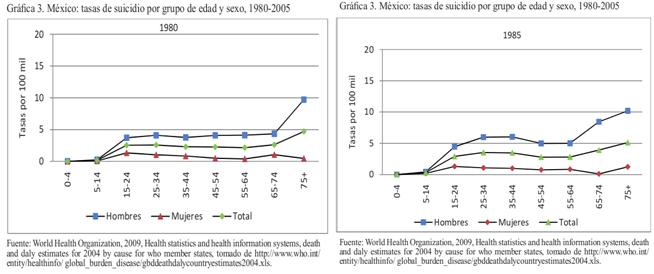
\includegraphics[width=10cm]{imagenes/1-suicidio/Graficas80_85.jpg}
\caption{Tasas de Suicidio por grupo de edad 1980 - 1985}
\end{figure}

\begin{figure}[hbtp]
\centering
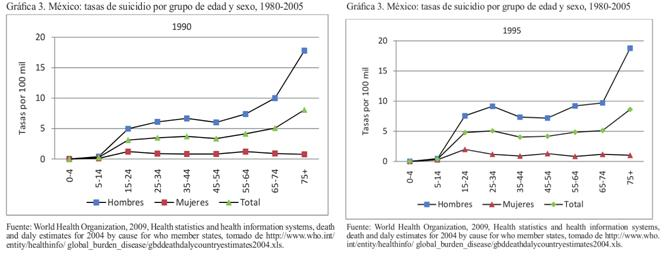
\includegraphics[width=10cm]{imagenes/1-suicidio/Graficas90_95.jpg}
\caption{Tasas de Suicidio por grupo de edad 1990 - 1995}
\end{figure}

\begin{figure}[hbtp]
\centering
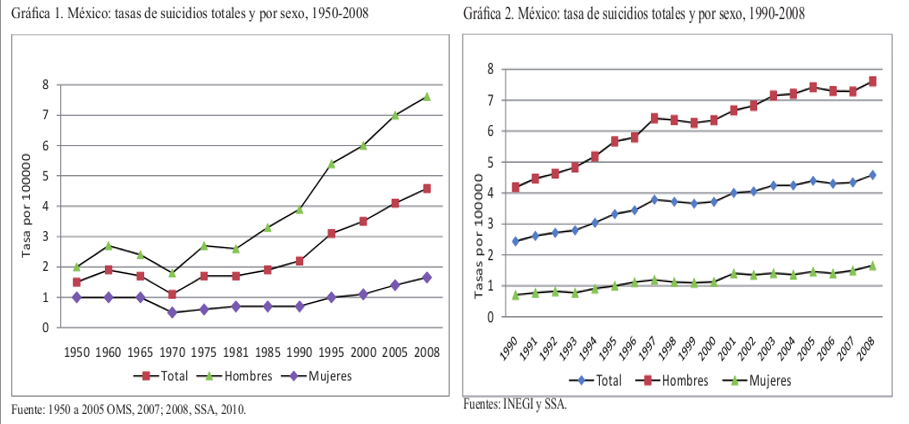
\includegraphics[width=10cm]{imagenes/1-suicidio/grafica1.png}
\caption{Tasas de suicidio totales y por sexo 1950-2008}
\end{figure}


\subsection{Confiabilidad en la recolección de Datos por el Inegi}
{
Aunque, en cada caso pueden variar la razón entre suicidios consumados e intentos de suicidio. Un estudio realizado por la Entrevista Internacional Compuesta de Diagnóstico de la OMS, que utiliza encuestas que incluyen una serie de preguntas estandarizadas acerca de la incidencia,  tiempo, métodos y tratamientos médicos (si hubo intentos de suicidios). Arroja un reporte disponible, el cual muestra la prevalencia de intentos de suicidio en períodos de 12 meses (recolectados desde el 2001 hasta el 2007) basado en 10 países de altos ingresos (9 de los cuales son usados como muestras representativas) con una muestra combinada de 52 484 individuos, seis países de ingresos medios (cuatro de ellos usados como muestras representativas) con una muestra combinada de 25 666 individuos y 5 países de bajos ingresos (uno de estos siendo usados como muestras representativas) con una muestra combinada de 31 227 individuos. (19). La prevalencia reportada de haber individuos que realizaron uno o más intentos de suicidio en el último año es de 3 por cada 1000 individuos (i.e. 3\%) en ambos hombres y mujeres de países con ingresos altos, 3 de cada 1000  hombres y 6 de cada 1000  mujeres en países de ingresos medios y 4 por cada 1000 hombres y mujeres de países de bajos ingresos. Aplicando la prevalencia en países de altos ingresos, medianos ingresos y bajos ingresos en adultos (18 años o más) de todos los países la prevalencia es que 4 por cada 1000 adultos han intentado suicidarse. Dada la prevalencia de suicidios consumados de 15.4 por cada 100 000 adultos (de 18 años o más), \emph{esto sugiere que por cada adulto que se ha suicidado es probable que hubiera más de 20 intentos de personas que han intentado el suicidio.}
\linebreak
\linebreak
Si vemos la gráfica siguiente, se puede notar los intentos de suicidio comparados entre Estados Unidos y México de 1999 y 2005.

\begin{figure}[hbtp]
\centering
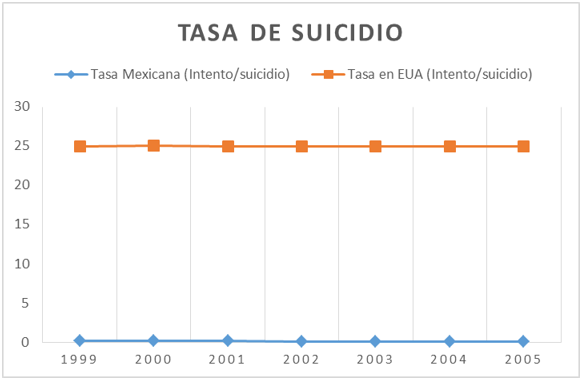
\includegraphics[width=10cm]{imagenes/1-suicidio/tabla2.png}
\caption{Comparativa entre México y Estados Unidos en Número de Intentos de Suicidio por Suicidio Consumado}
\end{figure}


Se necesita conocer los intentos de suicidio en particular, ya que no sólo producen un gran malestar mental y psíquico, sino que también son un antecedente fundamental de un posterior suicidio consumado. Con mucha frecuencia, un acto que llevó a una muerte por suicidio se ve precedido por una serie de intentos fallidos previos.\\

La recolección de los datos de las conductas suicidas es diferente a los datos de suicidio consumado, ya que se basa en gran medida en estadísticas recolectadas rutinariamente por las instancias oficiales a través del certificado de defunción. En el caso del intento de suicidio, no hay organismo que disponga de información veraz sobre este problema ya que no es obligatorio reportarlo, mucho menos el reportar la ideación o los planes suicidas. (Borges G, 2010)\\

}}
\section{Justificación}
{
Cada 40 segundos una persona muere en el mundo. La OMS ha lanzado un informe titulado " Prevención del Suicidio: un imperativo global ". Siendo el primer reporte de este tipo, pretende aumentar la conciencia en la salud pública sobre la importancia del suicidio y los intentos de suicidio, darle mayor prioridad a las acciones a favor de la prevención, alentar y respaldar a los países en desarrollar y fortalecer una estrategia con un acercamiento  comprehensivo y multisectorial. La prevención del suicidio requiere coordinación y colaboración entre múltiples sectores públicos y privados, sectores de salud y  sectores como el educativo,  empresarial, político, judicial, legal y medios de comunicación.  Estos esfuerzos deben ser comprehensivos, integrados y sinérgicos, dado que ningún intento aislado puede impactar a un problema tan complejo como el suicidio. \\

Para crear cambio social se requieren de tres importantes factores, la información (científico y de práctica informada), soporte público (voluntad política) y estrategia social como una respuesta nacional para cumplir los objetivos de prevención del suicidio. A pesar de que el suicidio es un problema de interés mundial, en México no se cuenta con la infraestructura para recabar información sobre el intento de suicidio. Dado que entenderlo provee información esencial para direccionar las acciones de prevención. Este estudio pretende ser una contribución significativa a la comprensión del comportamiento desde una perspectiva de la teoría de control.\\

Aunque la principal aplicación de la teoría de control es en el control de sistemas ingenieriles y control de procesos, las aplicaciones de esta rama van mucho más allá. La teoría de control es una útil herramienta para tratar sistemas donde existen lazos de realimentación, por ejemplo en la psicología, sociología, biología, sistemas financieros, control epidemiológico, entre otros.  Esta ciencia nos brinda una herramienta que pretendemos utilizar como una perspectiva innovadora que contribuya al entendimiento del comportamiento suicida de los mexicanos.
}
\section{Marco Teórico}
{
El suicidio es un acto con resultado letal, deliberadamente iniciado y realizado por el sujeto, sabiendo o esperando su resultado letal y a través del cual pretende obtener los cambios deseados.
\subsection{Tipo de Suicidio}
{
\begin{itemize}
\item Suicidio Egoísta: Individuos mal integrados en un grupo social
\item Suicidio Altruista: Se aplica a la excesiva integración a un grupo, siendo el suicidio el resultado de esta integración.
\item Suicidio Anómico: Se aplica a la desintegración social secundaria a la estabilidad social y a la pérdida de valores.
\end{itemize}
}
\subsection{Continuum suicida}
{
La conducta suicida cubre todo una serie de etapas llamadas continuum suicida. A continuación una breve explicación de en qué consiste.
\begin{itemize}
\item Idea de Muerte: Es la primera consideración a pensar que sería mejor estar muerto.
\item Idea (Fantasía) suicida: Autentico deseo de mejor morirse.
\item Plan (ideación) suicida: Mas allá del gusto, es que el individuo tenga un plan para concertarlo.
\item Gesto de suicidio: Cualquier acción por mínima que sea acorde a su deseo a morir.
\item Intentos de suicidio: Es el gesto más representativo que conlleva una acción con la que el individuo deseaba morir, pero no tuvo éxito.
\item Suicidio: El individuo concluye con su vida.
\end{itemize}
}
El suicidio es un problema global que ha prevalecido a través de los años, este problema también afecta a la comunidad mexicana. Distintos artículos científicos publicados por investigadores nacionales permitieron comenzar a entender más acerca de este fenómeno. En ellos se denotó que el suicidio en México es un problema que ha venido en incremento a nivel nacional, tal como en el artículo " El Suicidio en México " (HERNÁNDEZ-BRINGAS FLORES-ARENALES, 2011) que nos permite ver cómo ha evolucionado desde la década de los 50. Este artículo compara el suicidio con otros problemas de igual relevancia como son los homicidios y accidentes.
\linebreak
\linebreak
Al abordar el comportamiento suicida, nos referimos al rango de comportamientos que incluye desde la fantasía o idea de que sería mejor estar muerto, pasando por el planteamiento planeado, intento y hasta el suicidio consumado. En un artículo publicado en el 2010 en la revista de Salud Publica en México se muestran 3 estudios sobre la conducta suicida en México.
\begin{itemize}
\item La Encuesta Nacional de Epidemiología Psiquiátrica: Se aplicó a población no-institucionalizada, que tiene un hogar fijo, de 18 a 65 años de edad y que vive en áreas urbanas del país. Además se usó como instrumento de diagnóstico la versión computarizada de la Entrevista Internacional Compuesta de Diagnostico (WHO World Mental Health Survey Initiative versión of the CIDI-WMH-CIDI).
\item La Encuesta Mexicana de Salud Mental Adolescente: Se aplicó a 3005 adolescentes  de entre 12 y 17 años de hogares fijos en el área metropolitana de la Ciudad de México. Se evaluó con la versión de adolescentes computarizada de la Entrevista Internacional Psiquiátrica Compuesta (WMH-CIDI-A) diseñada para la Iniciativa “Encuestas Mundiales de Salud Mental ".
\item La Encuesta Nacional de Adicciones: Se realizó el estudio a un total de 50688 viviendas de todo el país; mediante entrevista directa en el hogar a un adulto de entre 18 a 65 años y a un adolescente de entre 12 a 17 años.
\end{itemize}
Los datos de las tres encuestas mencionadas han sido todo producto de investigaciones que realizó el Instituto Nacional de Psiquiatría Ramón de la Fuente Muñiz. Donde muestra los porcentajes por edad en los intentos de suicidio y planeación suicida en diferentes grupos en la República Mexicana.
\linebreak
\linebreak
En la figura 4.1 podemos ver como México se encuentra en la clasificación más baja (menor a 5 personas por cada 100 000 habitantes)

\begin{figure}[hbtp]
\centering
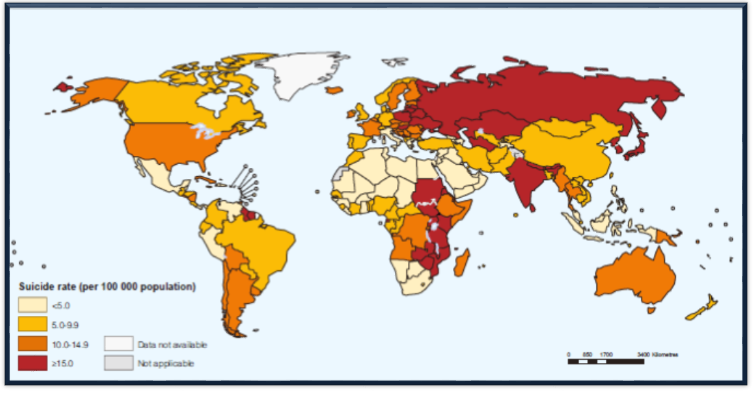
\includegraphics[width=14cm]{imagenes/1-suicidio/imagen1.png}
\caption{Tasas de suicidio a nivel mundial}
\end{figure}

\subsection{Factores de Riesgo}{
Los seres humanos podemos interactuar con factores de riesgo y factores protectores, (Un factor de riesgo es cualquier rasgo, característica o exposición de un individuo que aumente su probabilidad de sufrir una enfermedad o lesión y entiéndase por factores protectores aquellos que disminuyen la probabilidad de sufrir una enfermedad o lesión.),(OMS), los cuales agudicen la probabilidad del suicidio. Cabe mencionar que estos factores asociados al suicidio son diferentes cuando se habla de intentos de suicidio y suicidio consumado. Esta investigación se enfocara en los factores asociados al suicidio consumado.

A continuación, mencionaremos los factores definidos por la OMS en su último reporte y una explicación de lo que consta

\subsubsection{Sociedad}
{
\begin{itemize}
\item La disponibilidad de los medios utilizables para suicidarse.
\item Reportes inapropiados de los medios de comunicación aplicando una idea de Glamour que incrementa el riesgo a " copiar " o " imitar " la acción suicida.
\item El estigma de no pedir y buscar ayuda; también se incluye el estigma de los familiares y amigos de no ofrecer o hablar del tema con una persona aunque estén conscientes del problema por el que la persona atraviesa.
\item La dificultad de obtener acceso a la atención de Salud Pública por vivir en comunidades alejadas o la atención sea limitada.

\end{itemize}
}
\subsubsection{Comunidad}
{
\begin{itemize}
\item Desastres naturales, guerras y conflictos económicos y/o políticos.
\item Discriminación ante grupos minoritarios, por ejemplo: personas que acaban de salir de la cárcel, personas que declaran ser homosexuales o bisexuales, personas que son afectadas por el bullying o cyber – bullying, refugiados, inmigrantes, indigentes
\item Trauma o abuso: el cual puede ser un detonante para la depresión y conductas suicidas en personas que son vulnerables.
\end{itemize}
}
\subsubsection{Relaciones}
{
\begin{itemize}
\item La falta de apoyo por parte del grupo social o tener un sentimiento de soledad, puede llevar a la persona al aislamiento social, el cual es un factor de riesgo asociado con las personas de edad avanzada.
\item Conflictos con la pareja o con personas cercanas.
\item Perdida de pareja o de persona cercana.
\end{itemize}
}
\subsubsection{Del Individuo}
{
\begin{itemize}
\item Intento de suicidio previo; se considera de alto riesgo aunque el acto ocurriera un año antes.
\item Desorden mental: Algún trastorno psiquiátrico como depresión mayor, trastorno bipolar, trastorno de limite de la personalidad (Border line), esquizofrenia.
\item Abuso de alcohol y/o drogas llevando a problemas de depresión y acciones violentas. Generalmente es comorbido (concurrencia en el mismo individuo de un trastorno por el uso de sustancias y otro trastorno psiquiátrico).
\item Pérdida de empleo o situación económica alarmante.
\item Desesperanza: reconocida en una persona que tiene sentimientos de desánimo sobre el futuro, perdiendo su motivación y expectativas.
\item Dolor crónico por padecer, por ejemplo, cáncer, diabetes o VIH/Sida.
\item Historial Familiar de suicidio.
\item Factores genéticos y biológicos, por ejemplo bajos niveles de serotonina son asociados con intentos de suicidio en personas con algún trastorno psiquiátrico.
\end{itemize}
}}
\subsection{Intento Suicida}
{
También denominado para-suicidio, tentativa de suicidio, intento de autoeliminación o autolesión intencionada, se ha definido como aquel acto sin resultado de muerte en el que un individuo, de forma deliberada, se hace daño a si mismo.

El intento suicida es mas frecuente que el suicidio consumado con una prevalencia de 3.5\% y de ese porcentaje hasta 10\% terminara en suicidio.  (Bondy, B. et al Genetics of Suicide, Molecular Psychiatry. February, 2006. 11:336-351)
}
\subsection{Suicidio y uso de sustancias}
{
El suicidio es una de las principales causas de muerte entre personas con problemas por consumo de sustancias; debido a que comparados con la población general las personas con problemas de consumo de sustancias tienen 10 veces mas probabilidades de morir por un intento de suicidio y los usuarios de drogas intravenosas 14 veces mas (Wilcox,2004)\\

En México, información obtenida de la base de datos sobre la mortalidad de la célula forense del SISVEA en individuos registrados por el SEMEFO y notificados al Sistema de Vigilancia Epidemiológica de las Adicciones (SISVEA), informa que de las cuatro causas de muerte reportadas de 1994 a 2006, el suicidio ocupa el lugar número 4; y que la principal sustancia detectada en los casos de suicidio fue el alcohol (72.9\%)
}

\section{Pregunta de Investigación}
{
¿ Se puede modelar el comportamiento suicida de la Ciudad de México suponiendo que el sistema es dinámico y no lineal, utilizando un enfoque booleano?

\subsection{Objetivos}
{
\subsubsection{General}
{
Comprender el comportamiento suicida y desarrollar herramientas que ayuden a la prevención masiva de los causales que llevan a una persona a cometerlo.
}
\subsubsection{Especifico}
{
\begin{itemize}
\item Elaboración de un modelo matemático orientado a la descripción de los procesos dinámicos causales relacionados al suicidio.
\end{itemize}

\section{Metodología}
{
Abordamos al suicidio como un sistema dinámico. El comportamiento suicida se caracteriza por la interacción de sus elementos y las relaciones que hay entre ellos. Nosotros analizaremos a la persona suicida como un ente social que interacciona con el entorno, en el cual hay factores que afectan o ayudan a desarrollar el comportamiento del mismo. Realizamos un análisis booleano como primer método matemático, hacemos una tabla de verdad para analizar la interacción de los estados del vector, obtenemos las ecuaciones que generan esta tabla y simplificamos las ecuaciones.\\

Creamos un vector de estados booleanos con los factores de riesgo más importantes para suicidio consumado. Procedemos a buscar relaciones entre todos estos factores que lleven a 3 salidas propuestas, las cuales son:
\begin{itemize}
\item Suicidio.- Aquella persona a la que la influencia de los factores de riesgo y/o protectores le lleven a atentar contra su propia vida llevándolo a la muerte.
\item No suicidio.-Aquella persona a la que la influencia de los factores de riesgo y/o protectores le lleven a no atentar contra su vida.
\item Ciclo.- Aquella persona a la que la influencia de los factores de riesgo y/o protectores no le sean suficiente para llevarlos a la primera o segunda salida, pero tan inestable que a mínimos cambios en los factores el individuo se mueva a la primera o segunda salida.
\end{itemize}

Las ecuaciones booleanas nos dan las características principales del sistema propuesto, variables de mayor peso en el modelo y dependencias entre variables. Para esto, primeramente se propone un diagrama de estados del cual se pretende observar claramente las dependencias entre las variables del vector propuesto, después revisamos la correlación entre el encendido de las variables y los estados estables a los que el sistema converge.\\

Esta tabla y las ecuaciones encontradas se validarán con estadísticas de suicidio en México recopilados del INEGI y la Secretaría de Salud. Se desea validar estos modelos con bases de datos que sean bastas en características que nos permitan aproximarnos a las circunstancias de las personas que se suicidaron a partir de la edad, nivel de escolaridad, genero, nivel socioeconómico, región o método utilizado para el suicidio. \\

}
\section{Diagrama de flujo}
{
\begin{center}
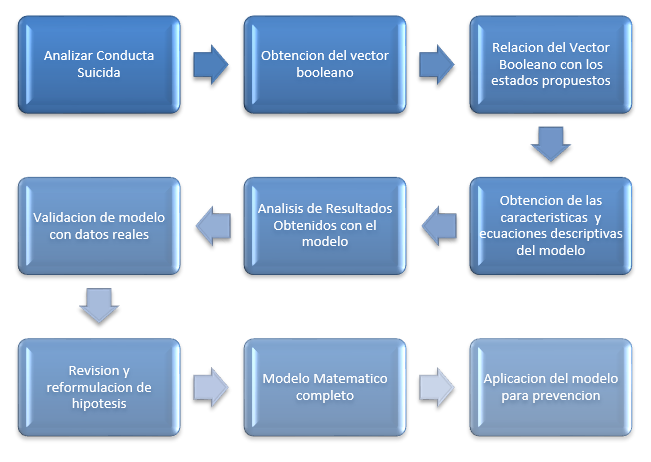
\includegraphics[width=10.5cm]{imagenes/1-suicidio/diagrama1.png}
\end{center}
}
\section{Resultados}
{
Nuestra hipótesis para el vector de estados del sistema son siete comportamientos que desencadenan un suicidio. La medición de los comportamientos individuales es exagerada o absoluta para tratarlos como variables booleanas. Estamos proponiendo describir cualquier tipo de conducta suicida por la combinación de los siguientes siete comportamientos \\.


\textbf{Agresividad:} Este comportamiento varía en género y entre culturas debido a la exposición de violencia del individuo. Esta exposición afecta claramente la forma en que tiende a resolver una situación personal y los métodos que elegiría para intentar suicidarse. Bajo esta perspectiva, la persona se considera a concebir la muerte y el suicidio como una solución " simple " a los problemas. Esto hace que el individuo sea mucho más eficaz en el intento de suicidio. Para ilustrar este comportamiento, podemos comparar la diferencia en la percepción de la muerte de un soldado, y un trabajador "normal" de oficina. \\

\textbf{Impulsividad:} Determina la rapidez con que una persona puede reaccionar a una situación de crisis y tomar acciones cuando son emocionalmente inestables. Aunque esto hace más difícil que un suicidio se consume debido al intento improvisado, este factor, mezclado en una persona agresiva puede convertirse en una peligrosa combinación. \\

\textbf{Depresión:} La desesperanza y la ansiedad están contenidas en este comportamiento. Se define como un estado de ánimo bajo y aversión a la actividad que puede afectar a los pensamientos, comportamientos, sentimientos y sentido de bienestar de una persona. Por ejemplo, la desesperanza puede afectar a las personas que tienen una enfermedad terminal o dolorosa. \\

\textbf{Incapacidad para hacer frente a los problemas:} Todo el mundo tiene problemas en diferentes contextos de su vida, algunas personas tienen problemas más grandes que otros. Este comportamiento describe la percepción de la persona a la gravedad de sus problemas, y la capacidad para lidiar con ellos. Esto se determina por el apoyo social que la persona tiene, la actitud del individuo, motivaciones y experiencia que se ocupan de problemas significativos.\\

\textbf{Sin miedo al suicidio:} Esta clasificación tiene dos comportamientos diferentes que afectan de una manera similar. Una de ellas es la aceptación cultura de suicidio. Por ejemplo, en un lado podemos tener una cultura en la que se castiga el suicidio, o prohibido por la religión, mientras que en el otro lado, para un suicidio Kamikaze puede ser una cuestión de honor. El segundo comportamiento es el miedo a la persona para intentar suicidarse, en su defecto, y hacer frente a las consecuencias negativas permanentes, como la persona que se dispara con una pistola en la cabeza y falla en suicidarse, pero queda con un grave daño en el cerebro, o un temor relacionado con el dolor que sufrirá durante el acto. \\

\textbf{Pérdida de pensamiento racional:} La pérdida de pensamiento racional puede ser debido a varias situaciones, como la dependencia de las drogas o una enfermedad mental, lo que hace que el individuo pierda contacto con la realidad. Este comportamiento cubre todas las causas posibles. Aunque el abuso de alcohol y la esquizofrenia son enfermedades enfermedades muy diferentes, estamos considerando para este análisis que ambas circunstancias ocasionan una perdida del pensamiento racional. \\

\textbf{Irresponsabilidad:} Dicho de otra manera, son las razones que el individuo tiene para vivir aparte de él mismo. Este puede ser el afecto emocional a los hijos, la familia, la contribución de la sociedad, la dependencia económica de cualquier ser querido o cualquier cosa que la persona considere importante para seguir viviendo, a pesar de su voluntad de querer suicidarse. \\

Es importante decir que los comportamientos se inspiraron en las herramientas, que en la actualidad, se usan para orientar especialistas de la salud en la investigación en sus pacientes para medir el riesgo de suicidio. Las herramientas para la medición de los factores de riesgo consultados incluyen la escala de riesgo suicida de Plutchik, la escala de Beck de intencionalidad suicida, el cuestionario de razones para vivir, escala de Beck de desesperanza y el modelo de Sad Person. Proponer comportamientos que pueden medirse con estas herramientas nos permitirá trabajar más tarde en una ecuación que incluirá el comportamiento no sólo para los estados booleanos, sino para una ecuación más realista que describa el comportamiento suicida. \\

Ahora que tenemos el vector de estado, se procede a analizar el sistema con la relación entre las variables. Hemos analizado todas las posibles combinaciones de comportamientos en la forma de una tabla de verdad. Procedemos en nuestra investigación proponiendo la decisión o estado estable de cada combinación de comportamientos, dicho de otra manera, si la persona elegiría el suicidio, no suicidio u oscilar en el ciclo límite posponiendo la decisión. A continuación, sobre la tabla de verdad propuesta, encontramos las ecuaciones booleanas que describen el sistema y las simplificamos. Las ecuaciones resultantes para cada una de las decisiones son las siguientes.\\

$\neg$ = Negación, $\vee$ = OR Lógico , $\wedge$ = AND Lógico\\

$x_1$=Irresponsabilidad\\
$x_2$=Depresión\\
$x_3$=Perdida del pensamiento Racional\\
$x_4$=No miedo al suicidio\\
$x_5$=No capacidad para lidiar con problemas\\
$x_6$=Impulsividad\\
$x_7$=Agresividad\\

Vector de estado: $x_1x_2x_3x_4x_5x_6x_7$\\

Ecuación de Suicidio:
${ (x }_{ 1 }\wedge { x }_{ 2 }\wedge { \neg x }_{ 3 }\wedge { x }_{ 7 })\vee { (x }_{ 1 }\wedge { x }_{ 2 }\wedge { \neg x }_{ 3 }\wedge { x }_{ 6 })\vee { (x }_{ 1 }\wedge { \neg x }_{ 3 }\wedge { x }_{ 4 }{ \wedge x }_{ 5 }\wedge { x }_{ 7 })\vee { (x }_{ 1 }\wedge { \neg x }_{ 3 }\wedge { x }_{ 4 }\wedge { x }_{ 6 }\wedge { x }_{ 7 })\vee { (x }_{ 1 }\wedge { \neg x }_{ 3 }\wedge { x }_{ 5 }\wedge { x }_{ 6 })\vee { (x }_{ 2 }\wedge { \neg x }_{ 3 }\wedge { x }_{ 4 }\wedge { x }_{ 5 })\vee { (x }_{ 2 }\wedge { \neg x }_{ 3 }\wedge { x }_{ 4 }\wedge { x }_{ 6 })\vee { (x }_{ 2 }\wedge { \neg x }_{ 3 }\wedge { x }_{ 4 }\wedge { x }_{ 6 })\vee { (x }_{ 2 }\wedge { \neg x }_{ 3 }\wedge { x }_{ 5 }\wedge { x }_{ 6 })\vee ({ \neg x }_{ 3 }\wedge { x }_{ 4 }\wedge { x }_{ 5 }\wedge { x }_{ 6 })$\\


Ecuación de no suicidio:
${ (x }_{ 1 }\wedge { x }_{ 3 }\wedge { x }_{ 4 }\wedge { x }_{ 5 })\vee { (\neg x }_{ 1 }\wedge { \neg x }_{ 2 }\wedge { \neg x }_{ 3 }\wedge { \neg x }_{ 4 })\vee { (\neg x }_{ 1 }\wedge { \neg x }_{ 2 }\wedge { \neg x }_{ 3 }{ \wedge \neg x }_{ 5 })\vee { (\neg x }_{ 1 }\wedge { \neg x }_{ 2 }\wedge { \neg x }_{ 3 }{ \wedge \neg x }_{ 5 })\vee { (\neg x }_{ 1 }\wedge { \neg x }_{ 3 }\wedge { \neg x }_{ 4 }{ \wedge \neg x }_{ 5 })\vee { (\neg x }_{ 2 }\wedge { \neg x }_{ 3 }\wedge { \neg x }_{ 4 }{ \wedge \neg x }_{ 5 })\vee { (\neg x }_{ 2 }\wedge { \neg x }_{ 3 }\wedge { \neg x }_{ 4 }{ \wedge \neg x }_{ 6 }{ \wedge \neg x }_{ 7 })\vee { (\neg x }_{ 2 }\wedge { \neg x }_{ 3 }\wedge { \neg x }_{ 5 }{ \wedge \neg x }_{ 6 })\vee { (\neg x }_{ 2 }\wedge { \neg x }_{ 3 }\wedge { \neg x }_{ 5 }{ \wedge \neg x }_{ 7 })\vee { (\neg x }_{ 3 }\wedge { \neg x }_{ 4 }\wedge { \neg x }_{ 5 }{ \wedge \neg x }_{ 6 })$\\


Ecuación ciclo límite:
${ (x }_{ 1 }\wedge { \neg x }_{ 3 }\wedge { \neg x }_{ 4 }\wedge { x }_{ 5 }\wedge { \neg x }_{ 6 }\wedge { x }_{ 7 })\vee({ \neg x }_{ 1 }\wedge { x }_{ 2 }\wedge { \neg x }_{ 3 }\wedge { x }_{ 4 }\wedge { \neg x }_{ 5 }\wedge { \neg x }_{ 6 })\vee { (\neg x }_{ 1 }\wedge { { \neg x }_{ 2 }\wedge \neg x }_{ 3 }\wedge { x }_{ 4 }{ \wedge x }_{ 5 }{ \wedge \neg x }_{ 6 })\vee { (x }_{ 2 }\wedge { { \neg x }_{ 3 }\wedge x }_{ 4 }\wedge { \neg x }_{ 5 }{ \wedge \neg x }_{ 6 }{ \wedge \neg x }_{ 7 })\vee { (x }_{ 2 }\wedge { { \neg x }_{ 3 }\wedge \neg x }_{ 4 }\wedge { x }_{ 5 }{ \wedge \neg x }_{ 6 })\vee { (\neg x }_{ 2 }\wedge { { \neg x }_{ 3 }\wedge x }_{ 4 }\wedge { x }_{ 5 }{ \wedge \neg x }_{ 6 }{ \wedge \neg x }_{ 7 })$\\

Para esta ecuación estamos tomando en cuenta que ser responsable, tener miedo al suicidio y tener habilidad para lidiar con problemas requieren del pensamiento racional. Entonces una persona que ha perdido el pensamiento racional, no puede ni tener ninguno de estos atributos, ni tener la voluntad de suicidatse. Aunque las enfermaddes mentales y el abuso de drogas son importantes factores a considerar en la conducta suicida, estas variables en un analisis booleano, no son consideradas dado que el individuo no es considerado lo suficientemente conciente como para autoagredirse esperando resultados fatales.\\

Ecuación No Racional:
$ ( \neg x_1 \wedge x_3) \vee (x_3\wedge \neg x_4) \vee (x_3 \wedge \neg x_5) $\\

A partir de las ecuaciones, construimos un circuito lógico y una interfaz gráfica que nos permite simular el comportamiento suicida a través de nuestro modelo.

\begin{center}
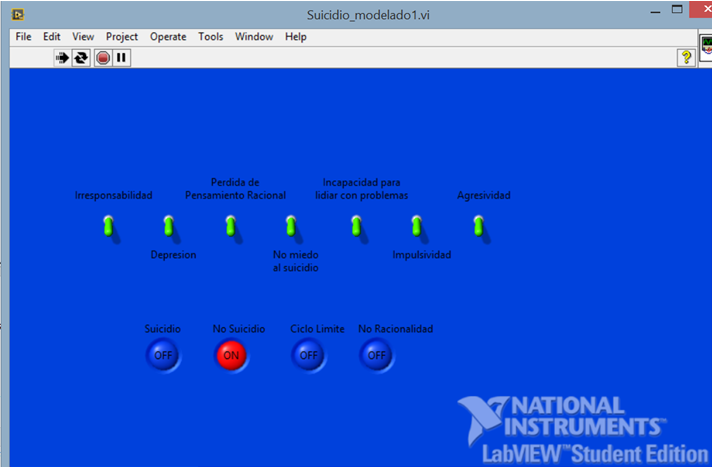
\includegraphics[width=12.5cm]{imagenes/1-suicidio/labview.png}
\end{center}
Además tenemos un mapa conceptual para analizar los resultados.
\begin{center}
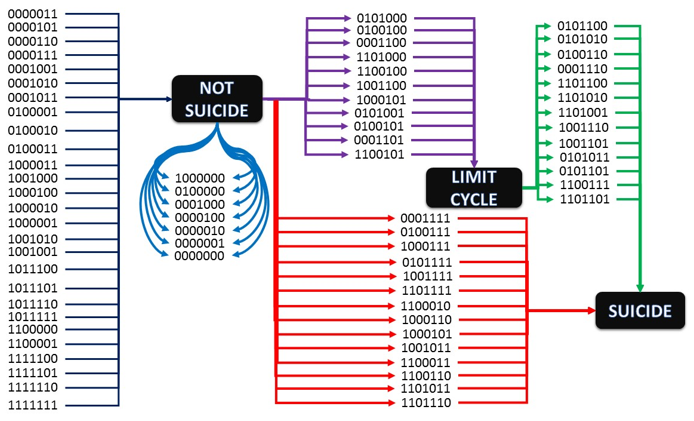
\includegraphics[width=12.5cm]{imagenes/1-suicidio/mapa.png}
\end{center}
Los resultados y conclusiones a los que llegamos son los siguientes:
\begin{itemize}
\item Se escogió a propósito la suma de productos, en vez del producto de sumas, dado que simplifica el análisis y basta con que una de las condiciones sea verdadera para que la conducta del individuo converja a algúna de las salidas propuestas.
\item El peso de la agresividad e impulsividad en las ecuaciónes siguiente nos dice que estas variables tienen pesos similares, dado que en el caso extremo si la persona es impulsiva, realiza el acto derivado de la situación y/o pérdida del valor de la vida a la que lo ha llevado la irresponsabilidad y la depresión. En este mismo contexto si la persona es agresiva tiende a ver el suicidio como una solución simple que la irresponsabilidad y la depresión le crearon.\\
${ (x }_{ 1 }\wedge { x }_{ 2 }\wedge { \neg x }_{ 3 }\wedge { x }_{ 7 })\vee { (x }_{ 1 }\wedge { x }_{ 2 }\wedge { \neg x }_{ 3 }\wedge { x }_{ 6 })$
\item De la misma manera podemos hacer referencia a los miniterminos siete y ocho presentan el mismo patrón entre la impulsividad y la agresividad.
\item De los miniterminos siete y nueve de la ecuación de suicidio podemos ver que se presenta una equivalencia de peso entre el "No miedo al suicidio" y la "habilidad de lidiar con problemas".
\item En los terminos seis y diez de la ecuación de suicidio vemos la equivalencia entre la "impulsividad" y "depresión" para las personas que "No tienen miedo al suicidio" y "No tienen habilidad para lidiar con los problemas".
\item Vemos también que en la ecuación de no suicidio, dado a que todos los términos están expresados en una connotación negativa, la mayoría de las variables aparecen negadas.
\item Haciendo una correlación de las variables con la salida del sistema vemos que:
\begin{enumerate}
\item La impulsividad (77\%), la depresión (70\%), No miedo al suicidio (70\%) y la incapacidad para lidiar con problemas (70\%) tienen la mayor relación con la salida del suicidio.
\item La depresión (63\%) y la incapacidad para lidiar con problemas (72\%) son las variables más relacionadas con el ciclo limite.
\item Mientras que el no suicidio tiene a todas las variables asociadas de una manera similar.
\end{enumerate}
\item Las variables de estado tales como depresión, no miedo al suicidio y la incapacidad para solucionar problemas tienen un comportamiento interesante. Las variables por si solas se mantienen en el estado " No suicidio " pero la combinación de dos de ellas lleva a la persona al estado “ Ciclo Limite ” donde la persona tiene la idea de suicidio, pero no ha cometido el acto. La unión de las estas tres variables hace que la persona salga del ciclo limite y llegue al estado “ Suicidio ”, demostrándonos cual importante son en el modelo y que tienen mucho peso cuando se piensa en la prevención del suicidio.
\item Podemos ver también, que la variable de estado “ impulsividad ” tiene peso en el modelo cuando la persona está en el estado “ Ciclo limite ”, ya que la “ activación ” de esta variable envía a una persona del estado “ Ciclo limite ” al estado “ Suicidio ”.
\item La variable de estado “ Agresividad ” no tiene mucha relevancia en el modelo, solo en casos específicos tiene el efecto de cambiar el estado en el que se encuentra una persona.
\item El cambio de estado desde “ No suicidio ” al estado “ Suicidio ” puede ser alcanzado sin la necesidad de pasar por el estado “ Ciclo Limite ”. Lo anterior nos ayuda a inferir que a una persona en segundos puede tomar la idea y pasar a la acción sin la necesidad de estancarse en un ciclo.
\item El estado “ suicidio ” no puede ser alcanzado si no se tiene al menos 3 variables de estado activas, eso nos dice que una persona necesita tener una mezcla de las variables de estado para llegar al punto de quitarse la vida. No es solo un factor el que sea importante, si no la combinación de ellos lo que hace la diferencia.
\item Podemos inferir de los resultados anteriores que en efecto, las ecuaciones encontradas reflejan las hipótesis que propusimos en la tabla de verdad.
\item El modelo carece de validación debido a que no se cuenta en México con suficiente información donde podamos corroborar los comportamientos y características que llevaron a una persona al suicidio.
\end{itemize}
}
\section{Bibliografia}
{
Borges Gilherme, H. J.-M. (2012). Prevalence and Identification of groups at risk for 12-month suicidal behaviour in the WHO World Mental Health Surveys. New York: Cambridge University Press.
\linebreak
\linebreak
HERNÁNDEZ-BRINGAS, H. H., FLORES-ARENALES, R. (2011). Scientific Electronic Library Online.
\linebreak
\linebreak
Organización Mundial de la Salud. (10 de Septiembre de 2014). World Health Organization, 2014. Recuperado el 19 de Septiembre de 2014, de http://www.who.int/mental\_health/suicide-prevention/world\_report\_2014/en/
}
}
% \end{document}


    \chapter{Benford's Law in Dynamical Systems}
    \paragraph{Emanuel Rocha Campos, Gerardo E. Cardona Sánchez}
    % \documentclass[paper=a4, fontsize=11pt]{scrartcl} % A4 paper and 11pt font size
%
% \usepackage{hyperref}% in order to use hyperlinks
% \usepackage[T1]{fontenc} % Use 8-bit encoding that has 256 glyphs
% %\usepackage{fourier} % Use the Adobe Utopia font for the document - comment this line to return to the LaTeX default
% \usepackage[english]{babel} % English language/hyphenation
% \usepackage{amsmath,amsfonts,amsthm} % Math packages
% \usepackage{graphicx}
% \usepackage{epstopdf}
% \DeclareGraphicsExtensions{.eps}
% \usepackage{subcaption}
%
% %\usepackage{lipsum} % Used for inserting dummy 'Lorem ipsum' text into the template
%
% %\usepackage{sectsty} % Allows customizing section commands
% %\allsectionsfont{\centering \normalfont\scshape} % Make all sections centered, the default font and small caps
%
% \usepackage{fancyhdr} % Custom headers and footers
% \pagestyle{fancyplain} % Makes all pages in the document conform to the custom headers and footers
% \fancyhead{} % No page header - if you want one, create it in the same way as the footers below
% \fancyfoot[L]{} % Empty left footer
% \fancyfoot[C]{} % Empty center footer
% \fancyfoot[R]{\thepage} % Page numbering for right footer
% \renewcommand{\headrulewidth}{0pt} % Remove header underlines
% \renewcommand{\footrulewidth}{0pt} % Remove footer underlines
% \setlength{\headheight}{13.6pt} % Customize the height of the header
%
% \numberwithin{equation}{section} % Number equations within sections (i.e. 1.1, 1.2, 2.1, 2.2 instead of 1, 2, 3, 4)
% \numberwithin{figure}{section} % Number figures within sections (i.e. 1.1, 1.2, 2.1, 2.2 instead of 1, 2, 3, 4)
% \numberwithin{table}{section} % Number tables within sections (i.e. 1.1, 1.2, 2.1, 2.2 instead of 1, 2, 3, 4)
%
% \setlength\parindent{0pt} % Removes all indentation from paragraphs - comment this line for an assignment with lots of text
%
% %----------------------------------------------------------------------------------------
% %	TITLE SECTION
% %----------------------------------------------------------------------------------------
%
% \newcommand{\horrule}[1]{\rule{\linewidth}{#1}} % Create horizontal rule command with 1 argument of height
%
% \title{
% \normalfont \normalsize
% \textsc{CINVESTAV, Automatic Control Department} \\ [25pt] % Your university, school and/or department name(s)
% \horrule{0.5pt} \\[0.4cm] % Thin top horizontal rule
% \huge Benford's Law in Dynamical Systems \\ % The assignment title
% \horrule{2pt} \\[0.5cm] % Thick bottom horizontal rule
% }
%
% \author{Emanuel Rocha Campos, Gerardo E. Cardona S\'anchez} % Your name
%
% \date{\normalsize\today} % Today's date or a custom date
%
% \begin{document}

% \maketitle % Print the title

%----------------------------------------------------------------------------------------
%	PROBLEM 1
%----------------------------------------------------------------------------------------

\section{Overview}
The purpose of this document is to present the results of simulations and experiments regarding the implementation of a physical dynamical system, in this case, an autonomous electronic circuit made in order to look for Benford's Law conformity of a physical quantity. 
The circuits that were chosen for this objective have various regions of operation and can be easily regulated, so an important amount of experiments and simulations were performed.
Conformity to Benford's Law was achieved, and the circumstances under which the satisfactory results were obtained are also described in this document. 
%------------------------------------------------

\subsection{Benford's Law}
Benford's Law, also called the First Digit Law refers to the frequency distribution of digits from a data source.  The first observation was made by Benford \cite{Benford38} who looked through various sources of data and found that in some data sets the number 1 repeated about 30\% of the time, while larger digits occur less frequently. \\

Benford's Law is the probability distribution for the mantissa with respect to base $b \in \mathbb{N} \setminus \{1\}$ given by $\mathbb{P}(\text{mantissa}_b \leq t)=\log_b t  \forall t \in [1,b]$ ; the special case dealt with in this document is that described by:\\
\begin{align*}
    \mathbb{P}(\text{first significant digit}_{10} = d) = \log_{10}(1+\frac{1}{d})\text{,   }d=1,...,9
\end{align*}


Today, conformity to this distribution is looked for in accounting fraud detection\cite{Nigrini97}, election data and genome data. Moreover, a relationship between the brain electrical activity and Benford's Law was encountered, and the researches noted that compliance with Benford's Law is influenced by the presence of the anesthetic sevoflurane, or destroyed by noise in the EEG\cite{Kreuzer14}.

The following are two examples where Benford's Law holds: the well known Fibonacci sequence, and population data from Mexico's Municipalities, obtained from INEGI.


\subsubsection{Fibonacci Sequence}
The Fibonacci sequence consists in the sequence: 1,1,2,3,5,8,13,21,34,55,89,144, ... ; where the sequence can be defined as the recurrence relation:

\begin{align*} f_n=f_{n-1}+f_{n-2}\end{align*}

Next, the most significant digit from the first 1000 Fibonacci numbers is obtained, and the frequency of repetition of number 1 as the first digit is calculated, the same can be done with number 2, and so on until number 9. Finally a plot of this frequency distribution against the distribution predicted by Benford's Law is presented.


\begin{figure}[h]
\centering
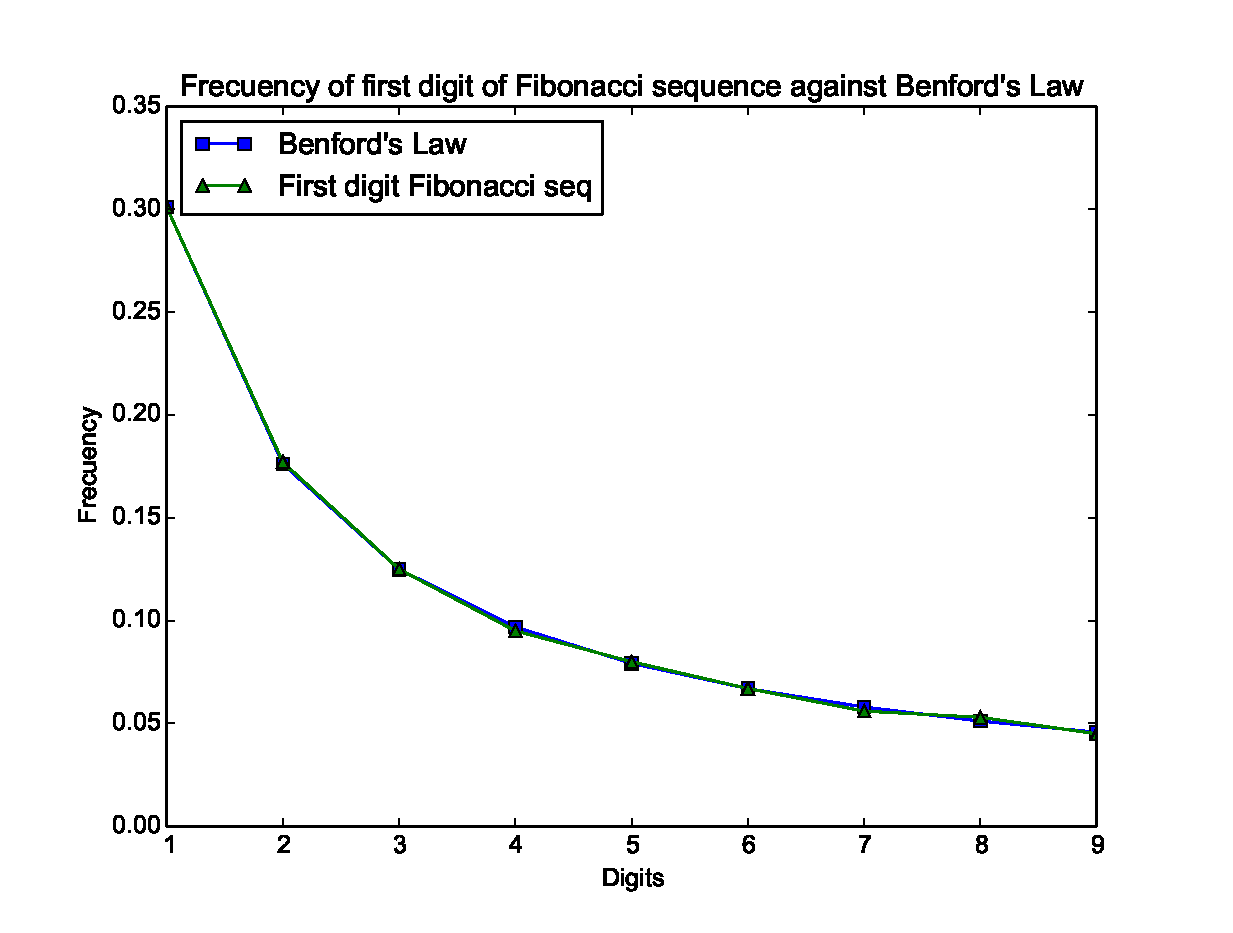
\includegraphics[scale=0.5]{imagenes/2-benford/benford_ex1}
\caption{Fibonacci Sequence against Benford's Law}
\end{figure}


\subsubsection{Mexico's Municipalities Population}
From the Mexico's National Institute of Geography and Statistics, INEGI, data from the 2010 census can be obtained. That year, 2351 Municipalities where censused and information is freely available at the institute web \href{http://www3.inegi.org.mx/sistemas/iter/entidad_indicador.aspx?ev=5}{page}.

As with the first example, the most significant digit of the population of each municipality was taken, and the frequency of repetition of each digit between 1 and 9 was compared with the prediction made by Benford's Law.

\begin{figure}[h!]
\centering
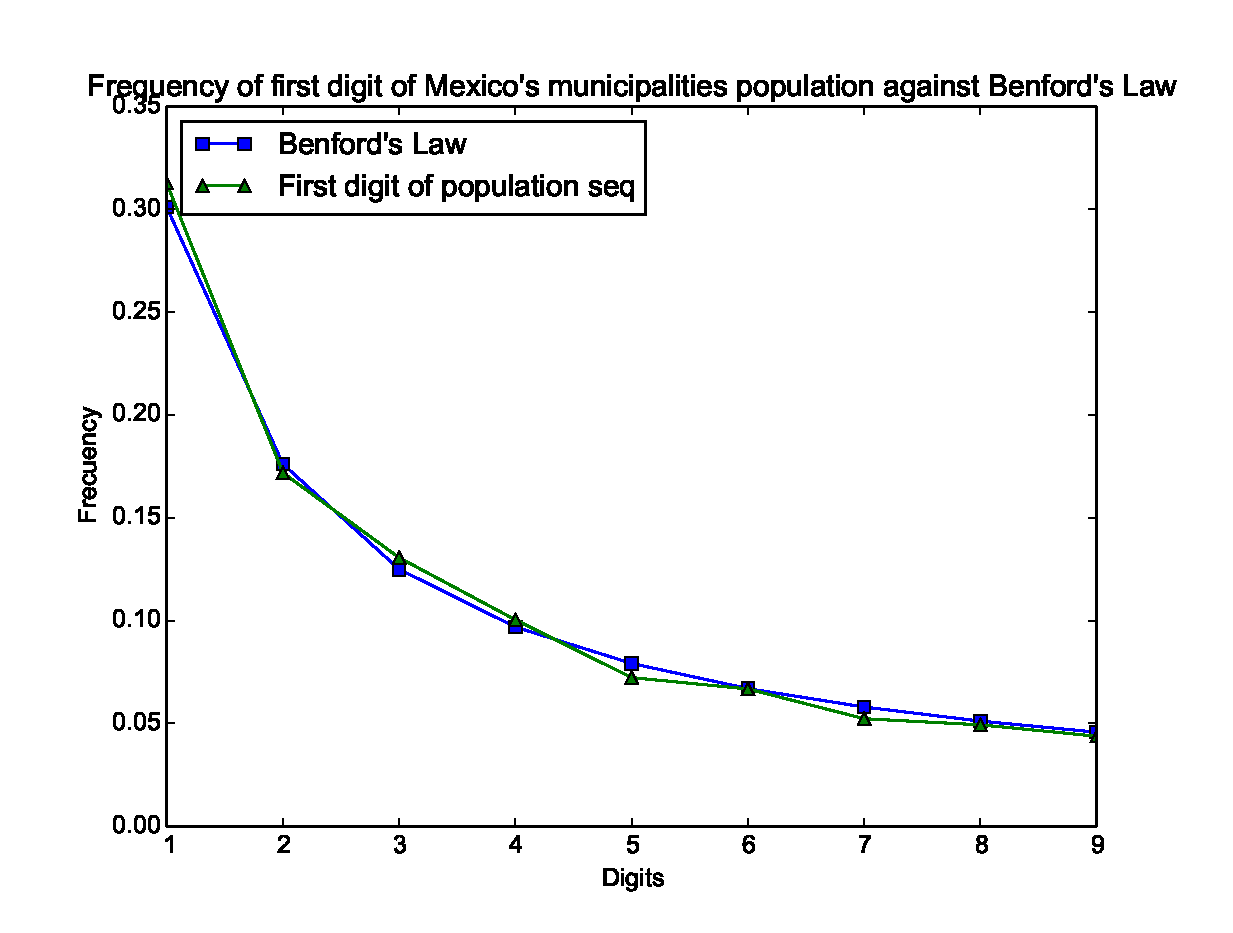
\includegraphics[scale=0.5]{imagenes/2-benford/benford_ex2}
\caption{Fibonacci Sequence against Benford's Law}
\end{figure}


\newpage
\subsection{Autonomous Circuits}
An Autonomous Circuit is a circuit that produces a time-varying output without having a time-varying input\cite{Kennedy95}. More formally:\\

An electronic circuit is described by a system of ordinary differential equations of the form:
\begin{equation*}
\dot{\mathbf{X}}(t)=\mathbf{F}(\mathbf{X}(t),t)
\end{equation*}
Where $\mathbf{X}(t)=(X_1(t),X_2(t),...,X_n(t))^T \in \mathbb{R}$ is called the \emph{state vector} and $\mathbf{F}$ is called the \emph{vector field}. $\dot{\mathbf{X}(t)}$ denotes the derivative of $\mathbf{X}(t)$ with respect to time.

If the vector field $\mathbf{F}$ depends explicitly on $t$, then the system is said to be \emph{non-autonomous}. If the vector field depends only on the state and is \emph{independent} of time $t$, then the system is said to be \emph{autonomous} and may be written in the simpler form:\\
\begin{equation}\dot{\mathbf{X}}=\mathbf{F}(\mathbf{X})\end{equation}


The time evolution of the state of an autonomous electronic circuit from an initial point $\dot{\mathbf{X}}$ at $t$=0 is given by\\

\begin{align*}\phi(\mathbf{X_0})=\mathbf{X_0}+\int_o^t\mathbf{F}(\mathbf{X}(\tau))d\tau &, t \in \mathbb{R}_+\end{align*}

The solution $\phi(\mathbf{X_0})$ is called a \emph{trajectory} through $\mathbf{X_0}$, and the set ${\phi(\mathbf{X_0}),t \in \mathbb{R}_+}$ is an \emph{orbit} of the system (1.1). The collection of maps ${\phi_t}$ that describe the evolution of the entire state space with time is called the \emph{flow}.

An autonomous electronic circuit is an example of a \emph{deterministic dynamical system}.

\subsection{Defining Chaos}
\emph{Chaos} is aperiodic long-term behavior in a determinisic system that exhibits sensitive dependence on initial conditions \cite{Strogatz14}
\begin{itemize}
\item \emph{Aperiodic long-term behavior} means that there are trajectories which do not settle down to fixed points, periodic orbits, or quasiperiodic orbits as $t$->$\inf$.
\item \emph{Deterministic} means that the system has no random or noisy inputs or parameters. The irregular behavior arises from the system's nonlinearity, rather than from noisi driving forces.
\item \emph{Sensitive dependence on initial conditions} means that nearby trajectories separate exponentially fast, i.e., that the system has a positive Lyapunov Exponent
\end{itemize}

\subsubsection{Lyapunov Exponent}
The lyapunov exponent of a dynamical system is a quantity that characterizes the rate of separation of infinitesimally close trayectories\cite{Parlitz92}.\\

Suppose that we let transients decay, so that a trajectory is \emph{on} the attractor. Suppose $\mathbf{\phi}(x,t)$ is a point on the attractor at time $t$, and consider a nearby point $\mathbf{\phi}(t)+\delta(t)$ where $\delta$ is a very small separation. It can be seen in the following figure, that  $\delta(t)$ grows. The two trajectories diverge with at a rate given by

$\lVert\delta(t) \rVert \ \lVert\delta_oo \rVert e^{\lambda t}$


\begin{figure}[h]
\centering
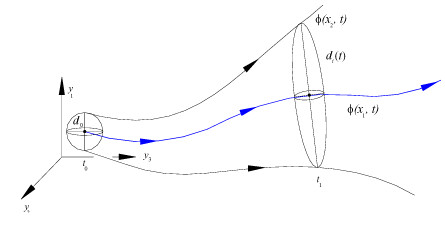
\includegraphics[scale=0.5]{imagenes/2-benford/Lyap_exp.jpg}
\caption{Neighboring trajetories separating exponentially fast with initial separation $\delta_0$ }
\end{figure}
When at least one Lyapunov exponent is positive the attractor possesses the property of sensitive dependence of initial conditions.


\subsubsection{Chua's Circuit}
\begin{itemize}\item \textbf{Chua's Oscillator}
\newline Leon Chua did research regarding Lorenz's equations\cite{Ayrom86}\cite{Kennedy95}, and deviced a chaotic electronic circuit with only one non-linear element, which is a 5-segment piecewise-linear resistor.


\begin{figure}[h]
\centering
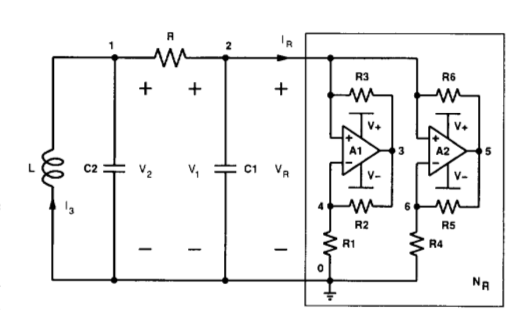
\includegraphics[scale=0.5]{imagenes/2-benford/chuas_circuit.png}
\caption{Schematic of Chua's Circuit }
\end{figure}

The dynamics of the system can be modeled by the system of three nonlinear ordinary differential equations:\\
\begin{align}
 \frac{dV_1}{dt}&=\frac{G}{C_1}(V_2-V_1)-\frac{1}{C_1}f(V_1)\\
 \frac{dV_2}{dt}&=\frac{1}{C_2}I_3-\frac{G}{C_2}(V_2-V_1)\\
 \frac{dI_3}{dt}&=-\frac{1}{L}V_2\\
\end{align}

with $G=\frac{1}{R}$ and $f(V_1)$ is given by:\\
\begin{align*}
\frac{G}{C1}V_2-\frac{G'_b}{C_1}V_1-(\frac{G_b-G_a}{C_1})E &\quad if \quad V_1< -E\\
\frac{G}{C1}V_2-\frac{G'_a}{C_1}V_1 &\quad if \quad -E\geq v1 \leq E\\
\frac{G}{C1}V_2-\frac{G'_b}{C_1}V_1-(\frac{G_a-G_b}{C_1})E &\quad if \quad V_1>E
\end{align*}
\item \textbf{Properties}
      \begin{enumerate}
       \item \textbf{Nonlinearity:} The system of equations has a nonlinear 2-terminal resistor described by a three segment piecewise-linear v-i characteristic shown in the following figure:


            \begin{figure}[h]
            \centering
            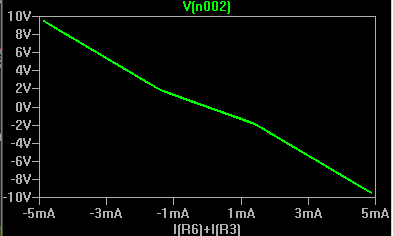
\includegraphics[scale=0.5]{imagenes/2-benford/v-i.png}
            \caption{v-i characteristic of the non-linear resistor }
            \end{figure}

      The piecewise-linear nature of the nonlinearity in Chua's Oscillator divides the state-space of the circuit into three distinct affine regions ($V_1<E$), ($\|V_1\|<E$) and ($V_1>E$)
      \item \textbf{Symmetry:}The piecewise-linear function is symmetric with respect to the origin, there exists three equilibrium points, at 0, $P_-$ and $P_+$. In the following figure, a double scroll Chua's attractor is shown. Since three equilibrium points are involved, this attractor is symmetric with respect to the origin\\

            \begin{figure}[h]
            \centering
            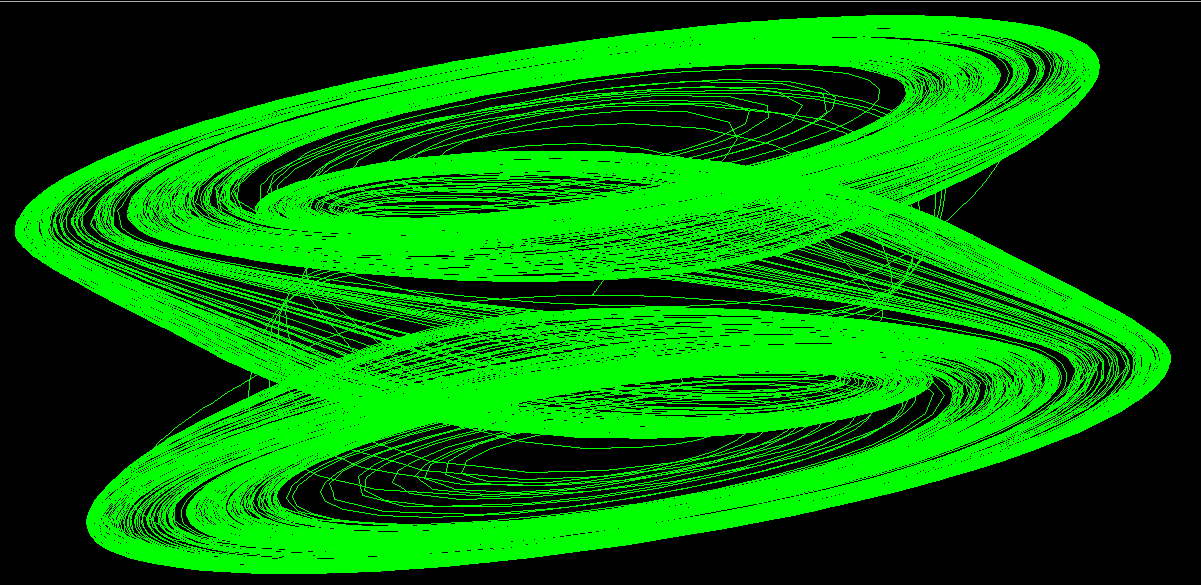
\includegraphics[scale=0.2]{imagenes/2-benford/chua_circuit.png}
            \caption{v-i characteristic of the non-linear resistor }
            \end{figure}
      \item \textbf{Dissipativity}
      \end{enumerate}
\end{itemize}


\newpage
\subsubsection{Takougang Circuit}
\begin{itemize}
\item \textbf{Three-dimensional autonomous system by Takougang et. al.}
    A three-dimensional autonomous system is presented by Sifei Takougang Kingni\cite{Takougang13}. The system exhibits chaotic bursting oscillations.\\
    The three-dimensional system is described as follows:\\
    \begin{align}
    \frac{dx}{dt}=-x+y\\
    \frac{dy}{dt}=xz-cy\\
    \frac{dz}{dt}=b-x^2-dz
    \end{align}

    where $b,c,d \in \mathbb{R}$
\item \textbf{Properties}
     \begin{itemize}
     \item \textbf{non-linearity:} Non-linearity given by the term $x^2$ and $xz$
     \item \textbf{symmetry:} Under the transformation defined by $(x,y,z) \rightarrow (-x,-y,-z)$, the system has a natural symmetry

     Next, we show that the system is symmetric.\\
     \textbf{Definition:}Let $f$ be a smooth function $f:\mathbb{R}^n \rightarrow \mathbb{R}^n$ and let\\
 \begin{align*}\mathbf{\dot{x}}=f(\mathbf{x})\end{align*}\\
 be a system of ordinary differential equations. In addition, let $\gamma$ be an invertible matrix. Then $\gamma$ is a \emph{symmetry} of the ordinary differential equation if \\
     \begin{align*}f(\gamma \mathbf{x})=\gamma f(\mathbf{x})\end{align*}

     Now, given the equation of the three-dimensional autonomous system, under the transformation $(x,y,z) \rightarrow (-x,-y,-z)$, to verify that this transformation is a symmetry of the autonomous equation, we observe that the symmetry is associated with the matrix $\gamma$ defined as\\
  \begin{align}
\gamma =
\begin{bmatrix}
-1 & 0 &0 \\
0 & -1 & 0\\
0 & 0 & 1
\end{bmatrix}
\end{align}

let \\  \begin{align}
\mathbf{\dot{x}}=f(\mathbf{x}) =
\begin{bmatrix}
-x + y \\
xz-cy\\
b-x^2-dz
\end{bmatrix}
\end{align}
with $\mathbf{x}^T=(x,y,z)$

Now, we proceed to show that $\gamma f(\mathbf{x})=f(\gamma \mathbf{x})$:\\
On the left hand side:
  \begin{align*}
\gamma f(\mathbf{x})&=
\begin{bmatrix}
-1 & 0 &0 \\
0 & -1 & 0\\
0 & 0 & 1
\end{bmatrix} \begin{bmatrix}
-x+y \\
xz-cy\\
b-x^2-dz
\end{bmatrix}\\
&=\begin{bmatrix}
x-y \\
-xz+cy\\
b-x^2-dz
\end{bmatrix}\\
\end{align*}

And now, on the right hand side:\\
  \begin{align*}
   f(\gamma \mathbf{x})&= f\left (\begin{bmatrix}
-1 & 0 &0 \\
0 & -1 & 0\\
0 & 0 & 1
\end{bmatrix} \begin{bmatrix}
x \\
y\\
z
\end{bmatrix} \right)\\
&=f\left ( \begin{bmatrix}
x \\
y\\
z
\end{bmatrix}\right )
&=\begin{bmatrix}
x-y \\
-xz+cy\\
b-x^2-dz
\end{bmatrix}
  \end{align*}

 Since the left hand side is equal to the right hand side, then $\gamma$ is a symmetry of the Three-dimensional Autonomous System. In other words, all solutions are either symmetric themselves, or have a symmetric partner
\item \textbf{Dissipativity} The system with the general condition for dissipativity (or Volume contraction):\\
         \begin{align*}\nabla V &= \frac{\partial(\frac{dx}{dt})}{\partial x}+\frac{\partial(\frac{dy}{dt})}{\partial y}+\frac{\partial(\frac{dz}{dt})}{\partial z}\\
&=-(1+c+d)
 \end{align*}

 So

\begin{align*}
V'(t)=-(1+c+d)V\\
V(t)V(0)e^{-(1+c+d)}t
\end{align*}

Thus volumes in phase space shrink exponentially fast
An explanation of dissipativity is given in \cite{Strogatz14} page 320.

\item \textbf{Fixed Points} The system has two types of fixed points:\\

      \begin{align*}
      0&=-x+y   \quad &\Rightarrow x=y\\
      0&=xz-cy   \quad&\Rightarrow z=c\\
      0&=b-x^2-dz  \quad&\Rightarrow x^2+dz=b \Rightarrow x=y=\sqrt{b-dc}
      \end{align*}
When $b \leq dc$ the fixed points for $x,y=0$ and $z=\frac{d}{b}$
When $b > dc$ the fixed points are $(\pm\sqrt{b-cd},\pm\sqrt{b-cd},c)$

\item \textbf{Sensitivity to initial conditons} Starting the system with slightly different initial conditions $(0, 0.1, 0)$ and $(0, 0.09, 0)$ we can see that after some time the two trajectories quickly diverge from each other



            \begin{figure}[h]
            \centering
            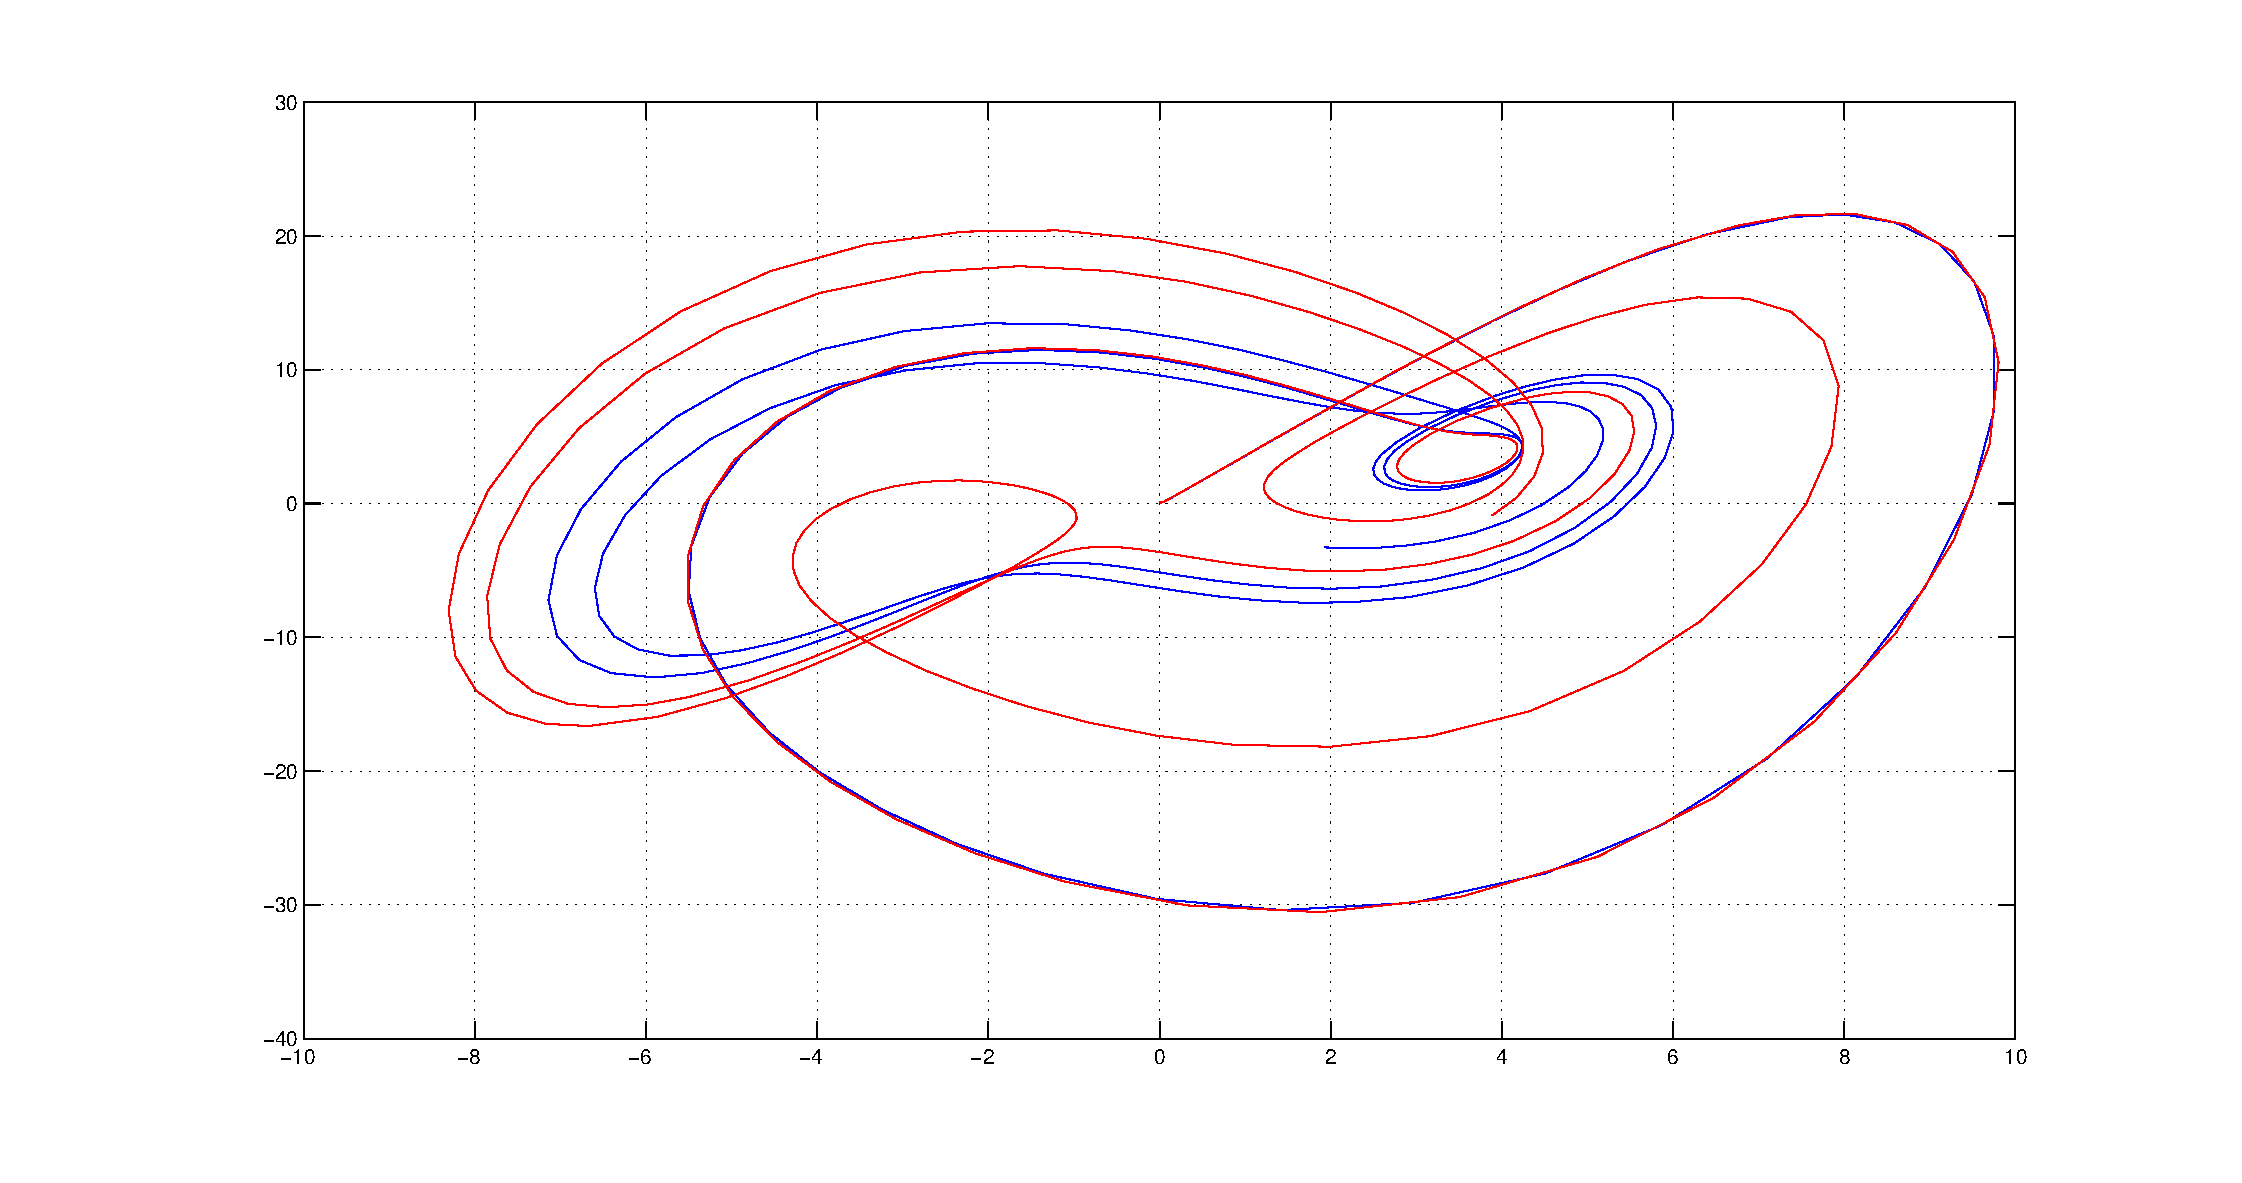
\includegraphics[scale=0.4]{imagenes/2-benford/in_cond.eps}
            \caption{Sensitivity to initial conditions in a Third Order Autonomous System}
            \end{figure}

     \end{itemize}
\end{itemize}

\cite{Takougang13} Shows that the system presents chaos of horseshoe type.


\newpage
\section{Simulations}
Simulations with Chua's System and the system proposed by \cite{Takougang13} were used to see if any of the system follows Benford's Law. On one hand we used Simulink and MATLAB in order to produce bifurcation diagrams and set up the dimensionless differential equations. On the other hand, we used a SPICE-based circuit simulator in order to get the systems in terms of electrical components.

\subsubsection{Chua's Circuit}
 \begin{itemize}
   \item \textbf{Physical Realization}
 The system describing chua's System
\begin{align*}
\frac{G}{C1}V_2-\frac{G'_b}{C_1}V_1-(\frac{G_b-G_a}{C_1})E &\quad if \quad V_1< -E\\
\frac{G}{C1}V_2-\frac{G'_a}{C_1}V_1 &\quad if \quad -E\geq v1 \leq E\\
\frac{G}{C1}V_2-\frac{G'_b}{C_1}V_1-(\frac{G_a-G_b}{C_1})E &\quad if \quad V_1>E
\end{align*}
is given by the following schematic
            \begin{figure}[H]
            \centering
            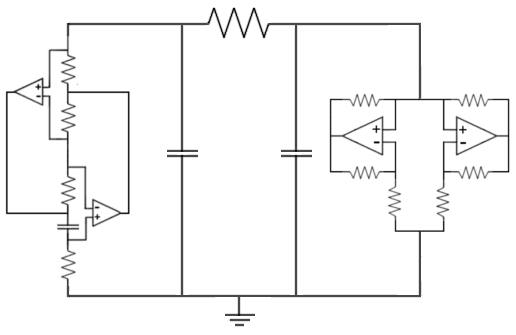
\includegraphics[scale=0.4]{imagenes/2-benford/chuas_circuit_realized.jpg}
            \caption{OP-Amp Based realization of Chua's Circuit}
            \end{figure}

With the Capacitors
C1=10nF
C2=100nF
and a 8mH Inductor given by the gyrator circuit.

   \item \textbf{Numerical Simulations}
   Using a spice based simulation software and MATLAB, several resistor values where tested, we constructed the bifurcation diagram and plotted for some R values
\begin{figure}
         \centering
            \begin{subfigure}[b]{0.4\textwidth}
            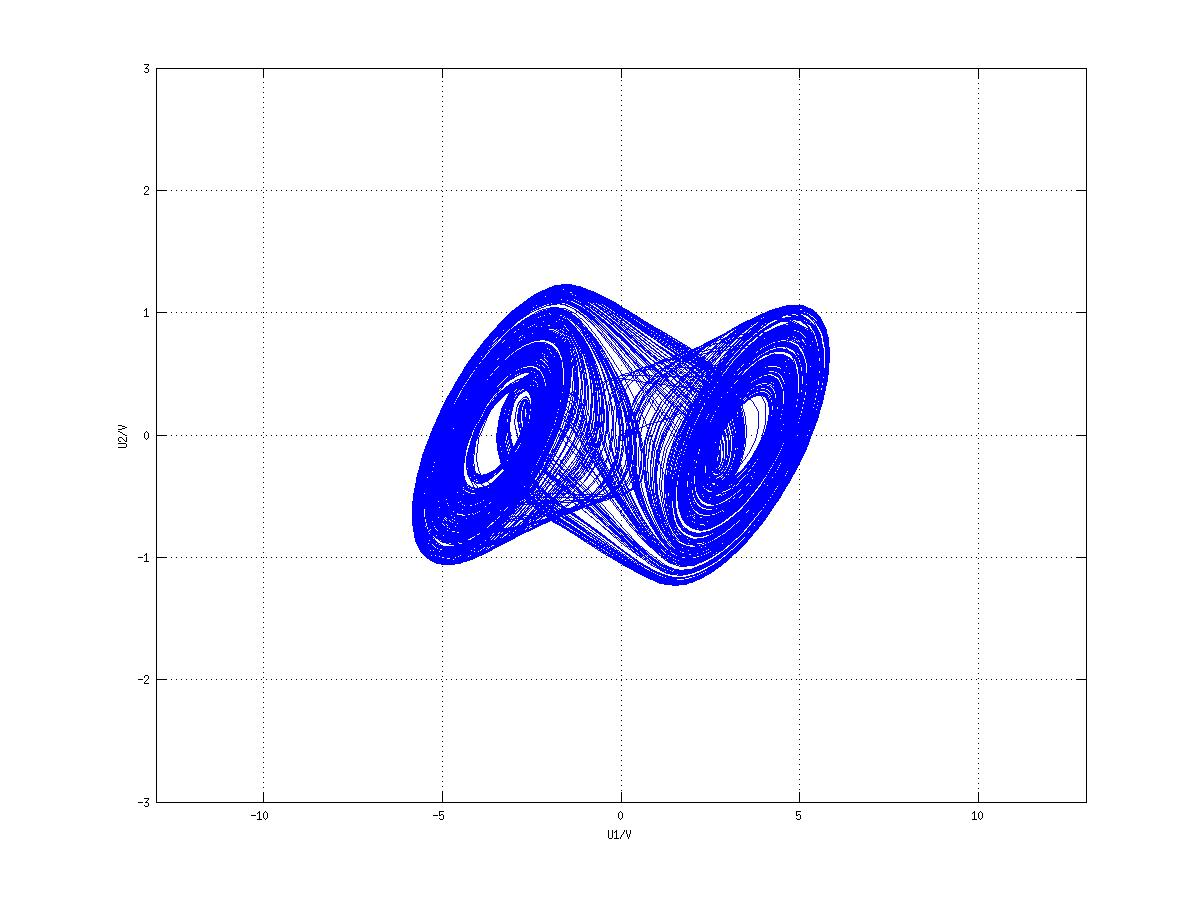
\includegraphics[width=\textwidth]{imagenes/2-benford/1785.jpg}
            \caption{V1-V2 plane for R=1785}
            \end{subfigure}
            \begin{subfigure}[b]{0.4\textwidth}
            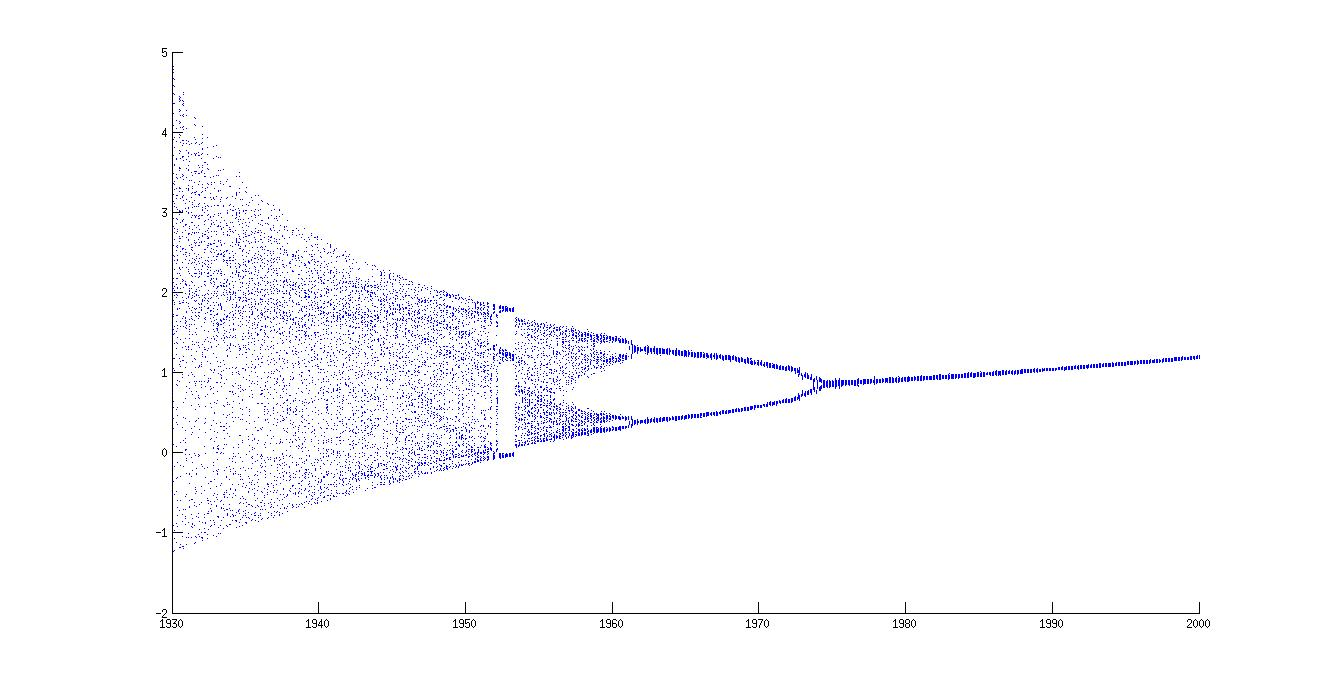
\includegraphics[width=\textwidth]{imagenes/2-benford/bifurcation_chua.jpg}
            \caption{Bifurcation Diagram for Chua's Circuit}
            \end{subfigure}
\end{figure}
   \item \textbf{Benford Analysis}
          The first digit distribution was determined from the voltage measured at the terminals of C1, using a resistance value of 1860$\Omega$, at that value, Chua's Circuit presented Chaotic Behaviour. The first digits (without leading zeroes) of the voltage values at discrete points were analyzed. We compared the first digit distribution of the dataset with the distribution given by Benford's Law using the Mean Absolute Deviation (MAD) proposed by \cite{Nigrini97}. We got a MAD value of 0.22, with a maximum of 0.15 in order to be conformant with Benford's Law.
            \begin{figure}[H]
            \centering
            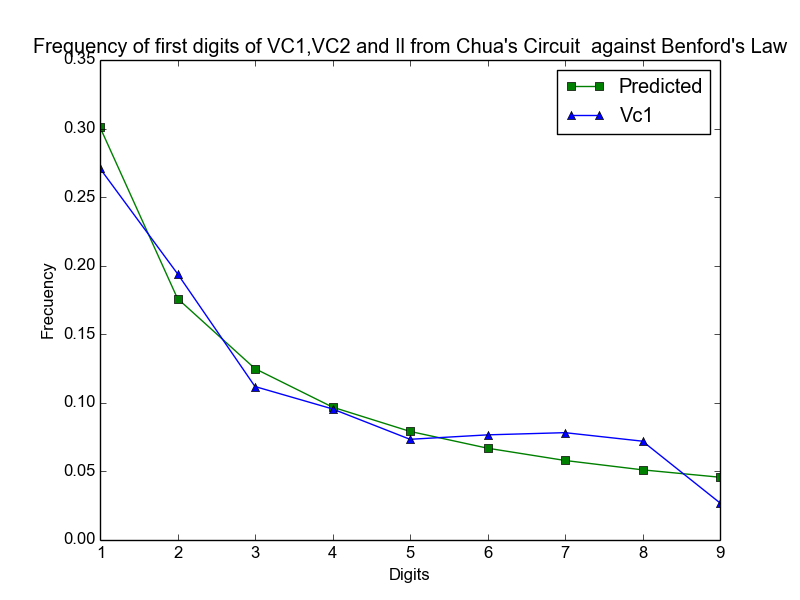
\includegraphics[scale=0.5]{imagenes/2-benford/chua_benford.png}
            \caption{OP-Amp Based realization of Chua's Circuit}
            \end{figure}
 \end{itemize}

\newpage
\subsubsection{Three-Dimensional Autonomous Circuit}
  \begin{itemize}
   \item \textbf{Physical Realization}
    The electronic circuit built to realise the system is shown in figure 2.4:
            \begin{figure}[H]
            \centering
            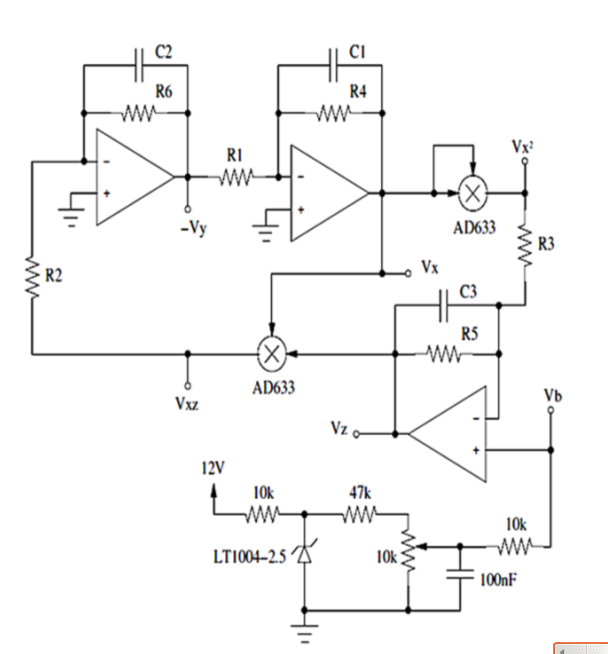
\includegraphics[scale=0.3]{imagenes/2-benford/Circuit2_schem.png}
            \caption{Circuit Schematic}
            \end{figure}
Voltages $V_x$,$V_y$ and $V_z$ are the output voltages of the operational amplifiers representing $x$,$y$ and $z$, $k_m=10V$ is the fixed constant of the AD633  multipliers, so the outputs of the multipiers are $V_{xz}=V_xV_z/k_m$ and $V_{x^2}=V_xV_x/k_m$.

            Substitution of resistor values into Eqs. (1.5),(1.6),(1.7) yields:

\begin{align}
\frac{dV_x}{dt}=\frac{1}{R_1C_1} \left ( V_y -V_x\frac{R_1}{R_4} \right )\\
\frac{dV_y}{dt}=\frac{1}{R_2C_2} \left ( \frac{V_xV_z}{k_m}-\frac{R_2}{R_6}V_y \right )\\
\frac{dV_z}{dt}=\frac{1}{R_3C_3} \left ( V_b\left ( 1+\frac{R_3}{R_5} \right )  -\frac{V_x^2}{k_m} - \frac{R_3}{R_5}V_z\right )
\end{align}

The values for resistors and capacitor used where: $R_1=0.5\text{ K}\Omega, \quad R_2=10\text{ K}\Omega, \quad R_3=10\text{ K}\Omega, \quad R_4=5\text{ K}\Omega, \quad R_5=1.15\textbf{\text{ M}}\Omega, \quad R_3=1\text{ M}\Omega, \quad C_1=100\text{ nF}, \quad C_2=100\text{ nF}, \quad C_3=10\text{ nF}, \quad V_b=10\text{ K}\Omega$
   \item \textbf{Numerical Simulations}
We used SIMULINK in order to model the system and MATLAB to create the bifurcation diagram.
            \begin{figure}[H]
            \centering
            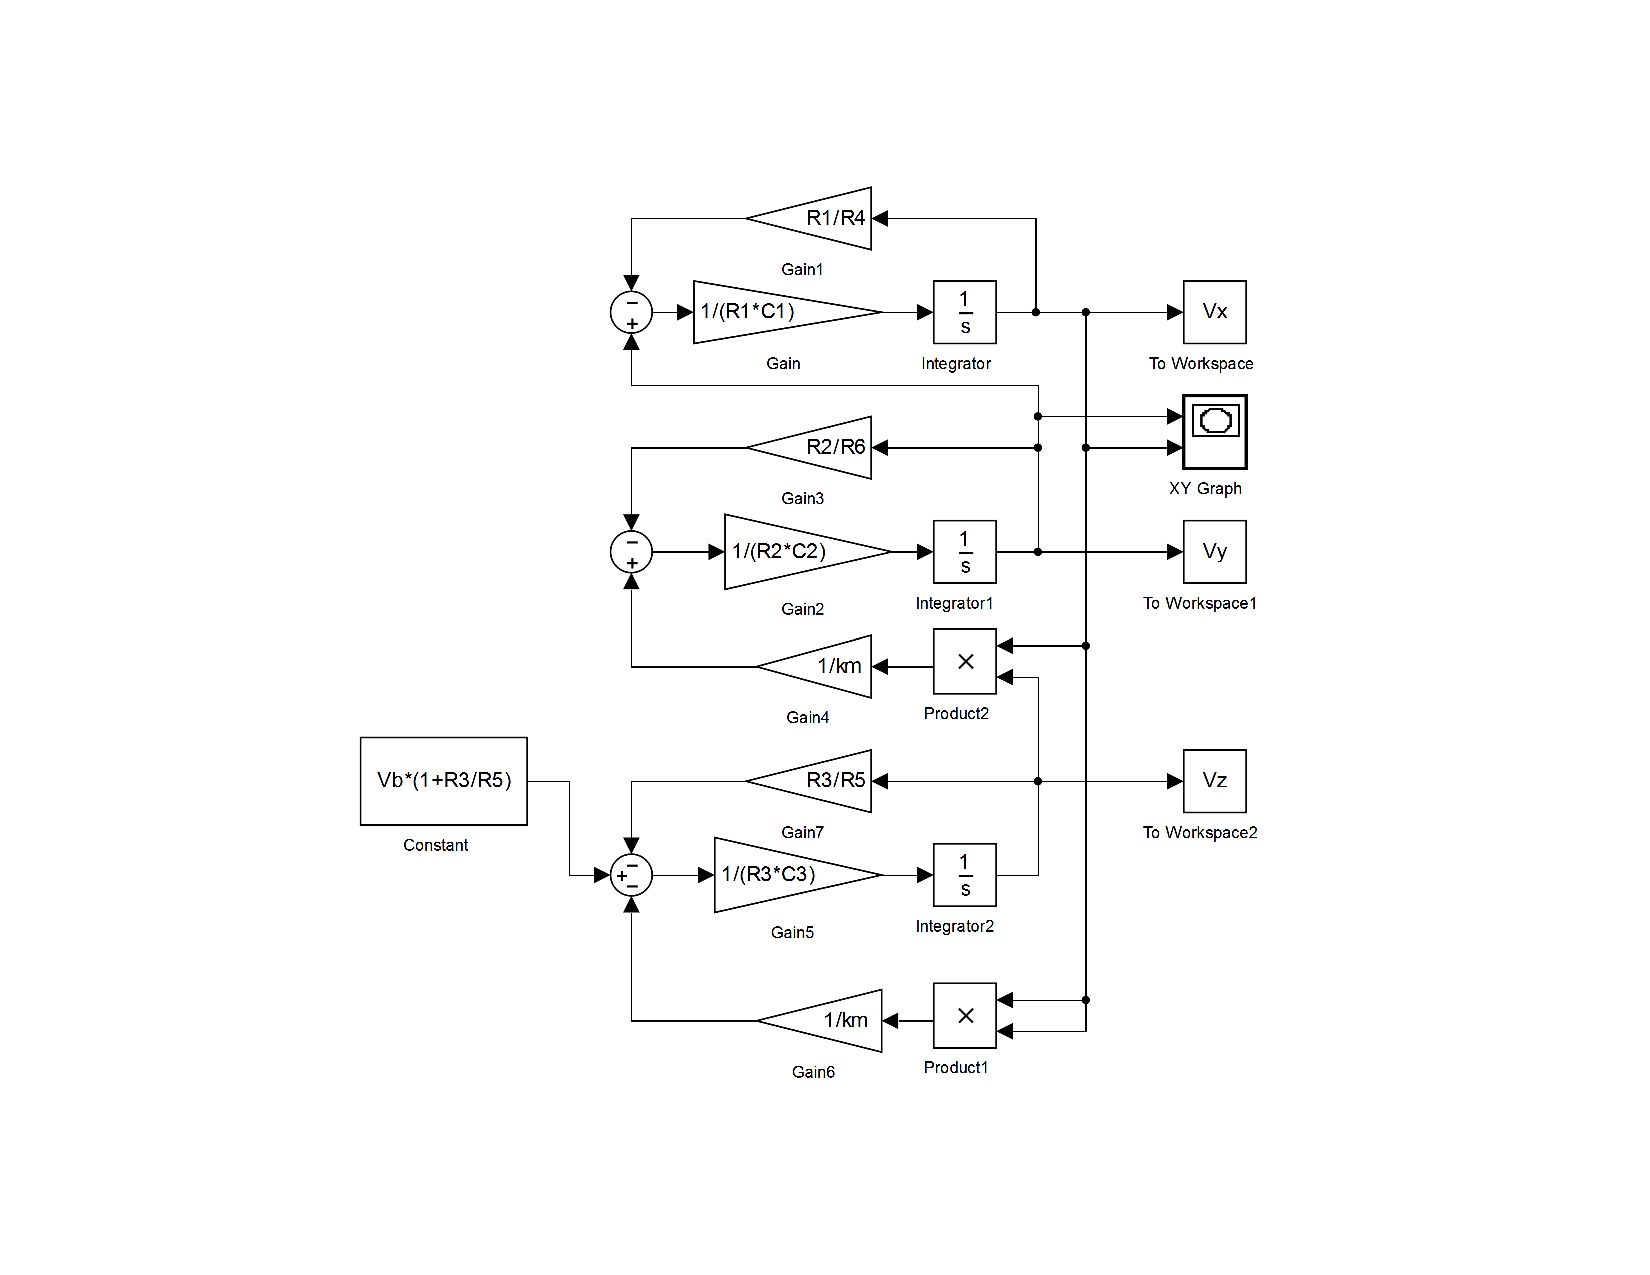
\includegraphics[scale=0.4]{imagenes/2-benford/shilkinovsimu.png}
            \caption{Simulink simulation}
            \end{figure}
The response of the syste with the parameters indicated above is given by figure 2.5:

\begin{figure}[H]
         \centering
            \begin{subfigure}[b]{0.4\textwidth}
            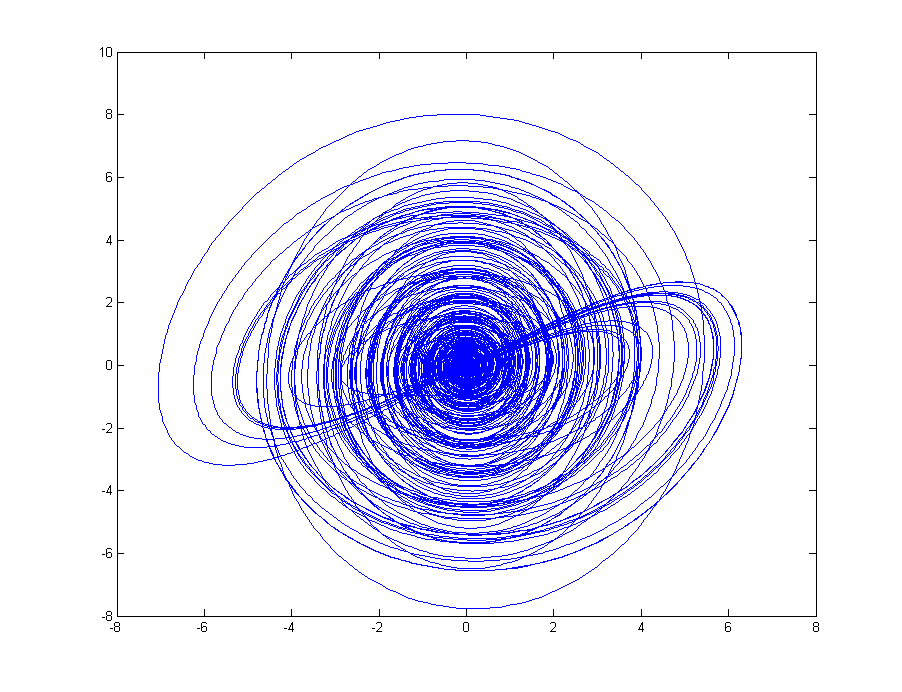
\includegraphics[width=\textwidth]{imagenes/2-benford/shilkino_resp.png}
            \caption{V1-V2 $V_x$ vs $V_y$ plot}
            \end{subfigure}
            \begin{subfigure}[b]{0.8\textwidth}
            \includegraphics[width=\textwidth]{imagenes/2-benford/bif_shil_osc_z.eps}
            \caption{Bifurcation Diagram varying b}
            \end{subfigure}
\end{figure}

Bifurcation diagram for the z value

   \item \textbf{Correspondence with Benford's Law} The same methodology used in Chua's Circuit was used with this circuit, taking measurements from $V_y$ and using the MAD test to verify conformity with the First Digit Distribution

            \begin{figure}[H]
            \centering
            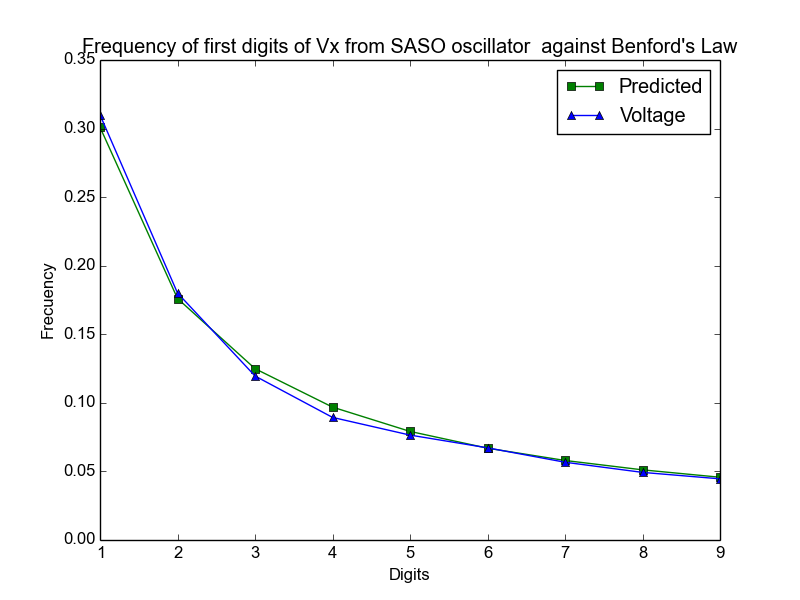
\includegraphics[scale=0.4]{imagenes/2-benford/Sh_vy.png}
            \caption{$V_x$ against Benford's Law}
            \end{figure}
For different values of d, we did a table with the respective first digit frequencies (10000 samples)  and MAD test.

\begin{center}
  \begin{tabular}{ c | c | c | c | c | c | c }
    \hline
    Leading digit  & Benford Distribution & d=1/23 &d=0.03 &d=0.01& d=0.001 &d=0.00001 \\ \hline
1&		0,3010&	0,3296&	0,3132&	0,3166&	0,2792&	0,3108\\ \hline
2&		0,1760&	0,1787&	0,1800&	0,1801&	0,1707&	0,1781\\ \hline
3&		0,1249&	0,1111&	0,1142&	0,1196&	0,1209&	0,1230\\ \hline
4&		0,0969&	0,0856&	0,0910&	0,0894&	0,0904&	0,0941\\ \hline
5&		0,0791&	0,0727&	0,0791&	0,0765&	0,0754&	0,0731\\ \hline
6&		0,0669&	0,0604&	0,0647&	0,0672&	0,0670&	0,0691\\ \hline
7&		0,0579&	0,0581&	0,0602&	0,0567&	0,0596&	0,0565\\ \hline
8&		0,0511&	0,0565&	0,0511&	0,0493&	0,0515&	0,0496\\ \hline
9&		0,0457&	0,0473&	0,0465&	0,0446&	0,0415&	0,0457\\ \hline
MAD&  & 0,0085&	0,0042&	0,0044&	0,0053&	0,0031\\ \hline

  \end{tabular}
\end{center}
We noticed strong agreement given by Nigrini\cite{Nigrini97}, next, we built the circuits and do tests measuring voltages.

 \end{itemize}


\newpage
\section{Experimental Results}
\subsubsection{Chua's Circuit}
 \begin{itemize}
  \item \textbf{Methodology}
We constructed the circuit using 4 TL082 I.C.'s and commercial resistors with the values used during simulation, Trimmer resistors to be able to move the resistor values of R.

            \begin{figure}[h]
            \centering
            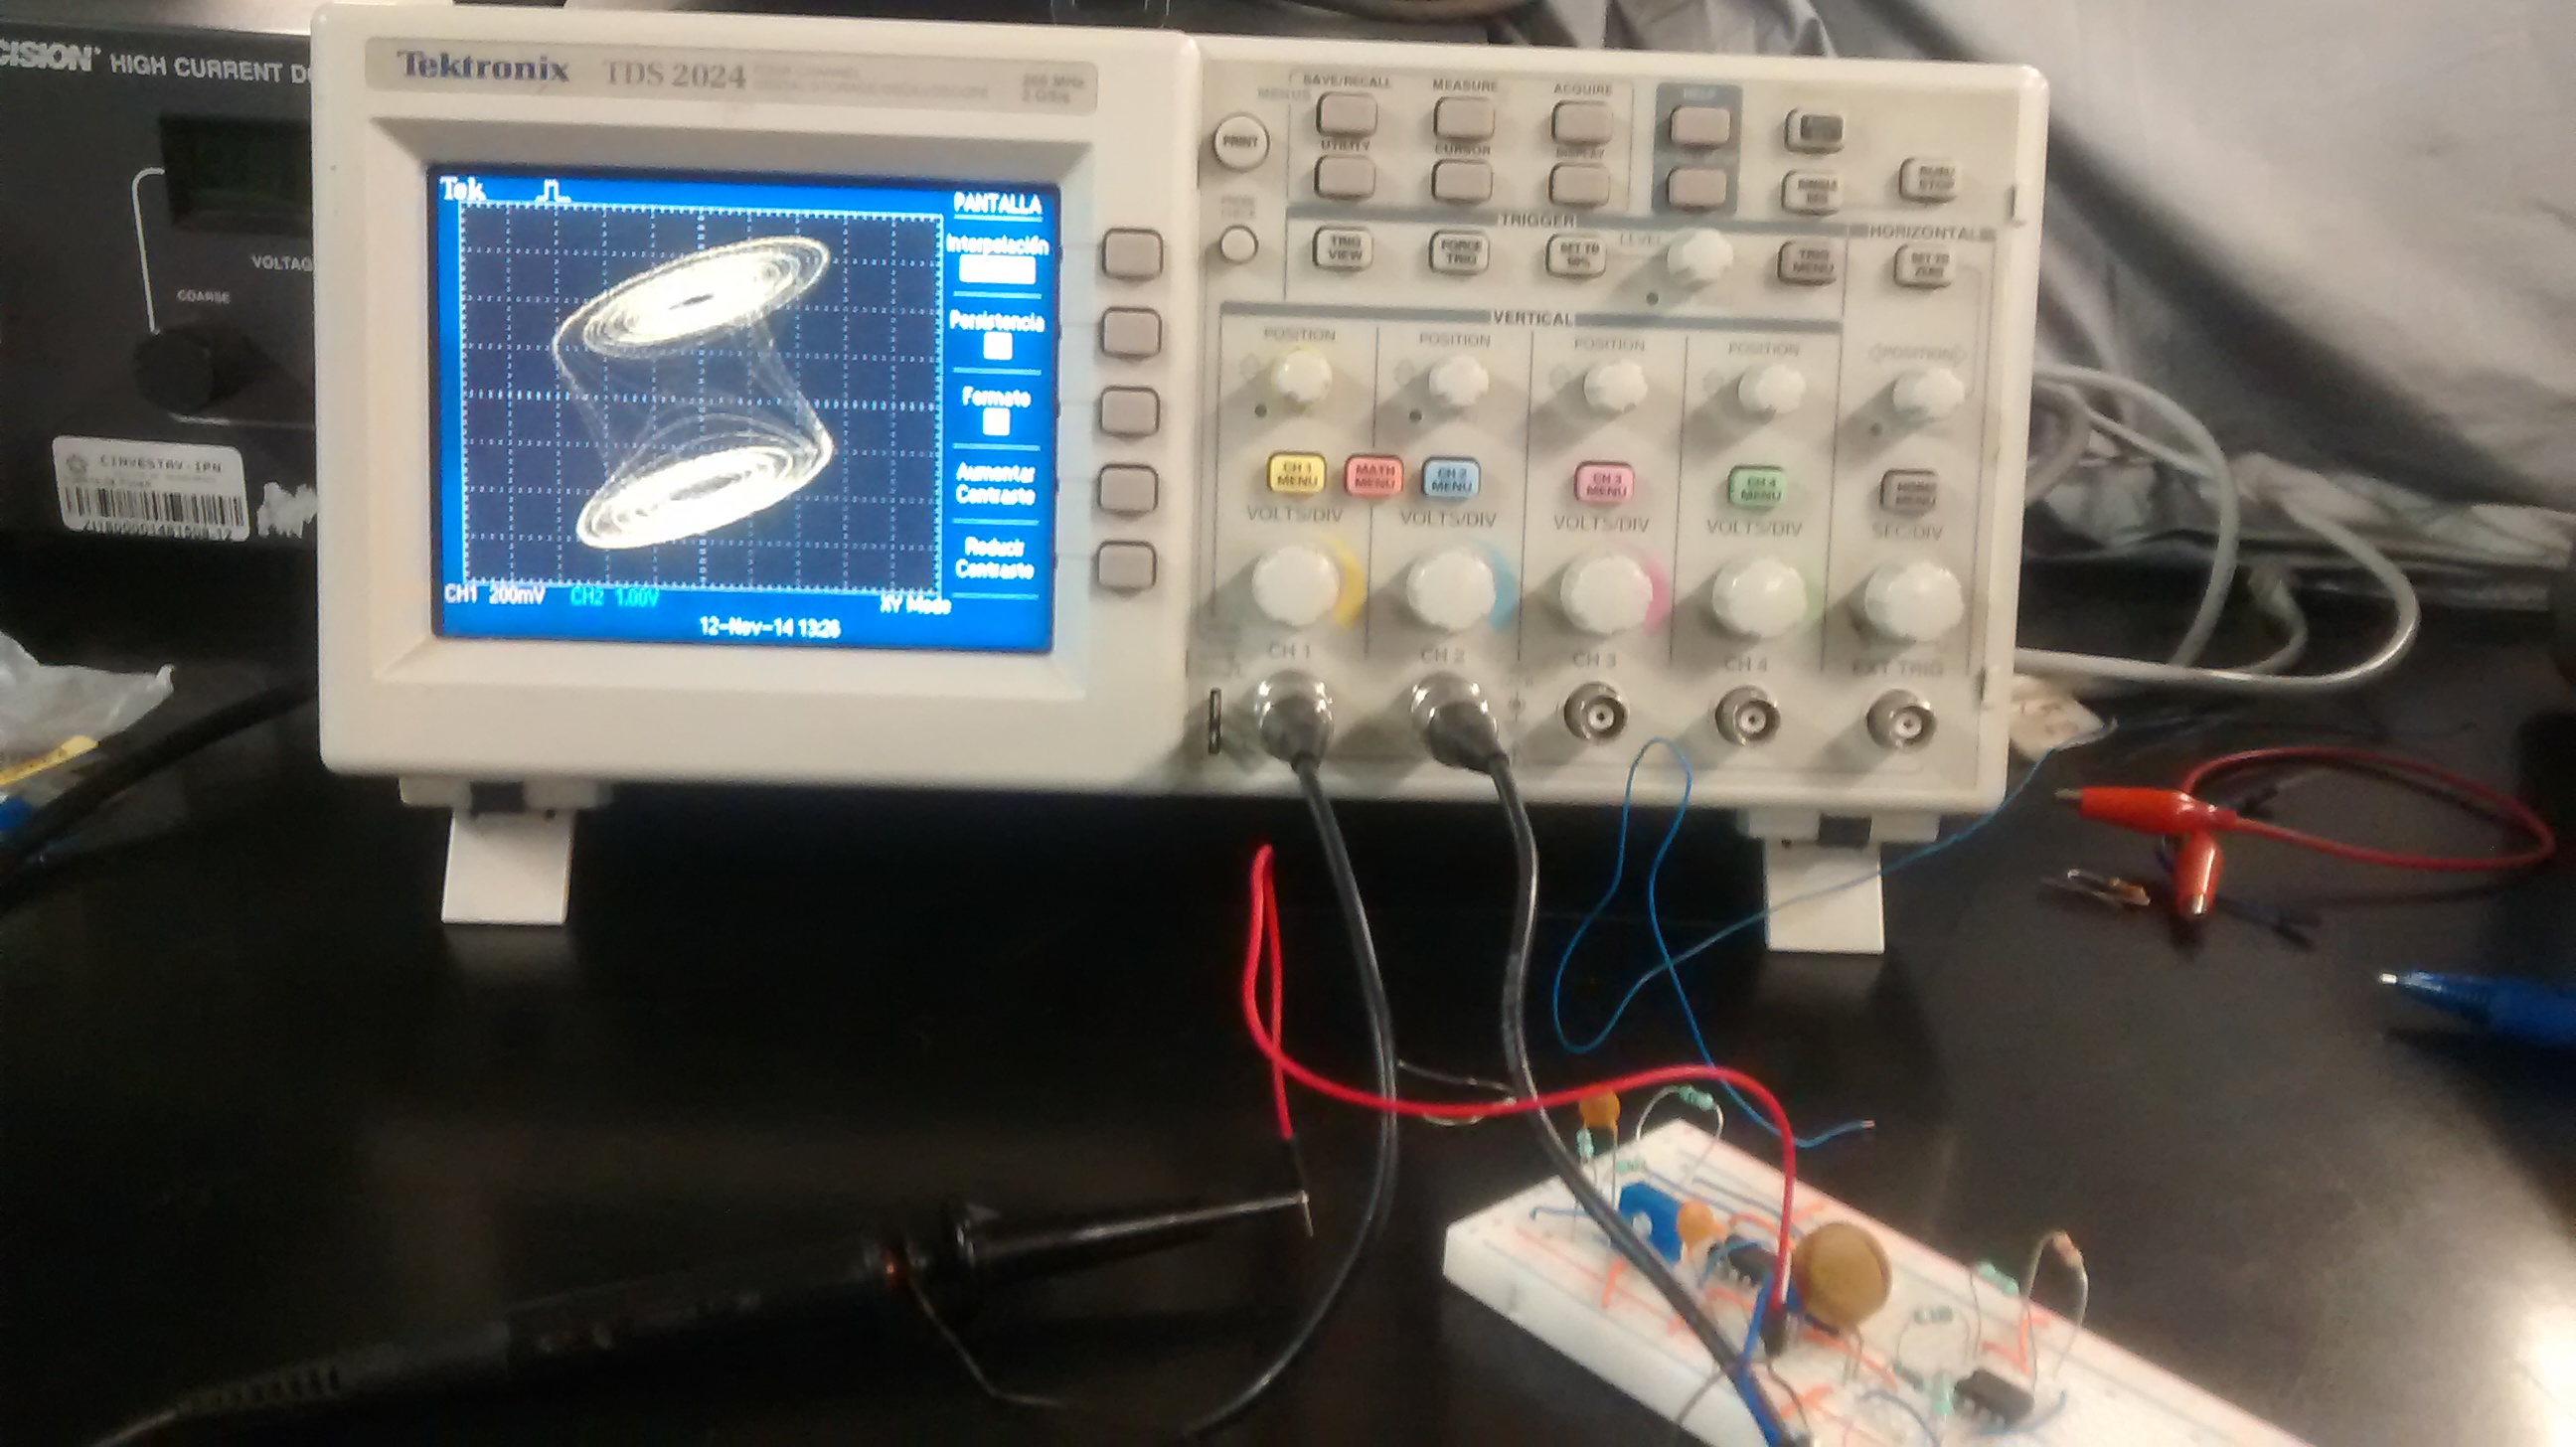
\includegraphics[scale=0.1]{imagenes/2-benford/chua_breadboard.jpg}
            \caption{Chua's System Breadboard}
            \end{figure}
We used two oscilloscope probes to measure the voltage from the two capacitors, and did our measurements with  a Tektronix DS201 Oscilloscope with a direct method sampling.

 The first digit distribution was determined from the voltage measured at the terminals of C1,varying R from 1700$\Omega$ to 1900$\Omega$in $25\Omega$ intervals, values in which Chua's Circuit presented chaotic behaviour. The first digits (without leading zeroes) of the voltage values at discrete points were analyzed, the oscilloscoped allowed us to take 2000 samples from a 250 $\mu$s period. We compared the first digit distribution of the dataset with the distribution given by Benford's Law using the Mean Absolute Deviation (MAD) proposed by \cite{Nigrini97}.



  \item \textbf{Results}
We put a table with the MAD results at each value of R:
\begin{center}
  \begin{tabular}{ c | c | c }
R & VC1 & VC2\\
1700 & 0.0265740826252 &0.0941252615083\\ \hline
1725 &  0.0308583854254& 0.0894910362566\\ \hline
1750 & 0.0225012003889 & 0.0937811348396\\ \hline
1775 &  0.0213932963068 & 0.0894482136018\\ \hline
1800 &  0.0515553953624& 0.0817178075546\\ \hline
1825 & 0.0620516456615 &0.0757908400412\\ \hline
1850& 0.0801858066881 &0.0616474503737\\ \hline
1875 & 0.0864648516751& 0.0566898036332\\ \hline
1900 &0.0848654579991 &0.0477795566486\\ \hline


  \end{tabular}
\end{center}

The closest value we got was with R=1775 measuring VC1
            \begin{figure}[h]
            \centering
            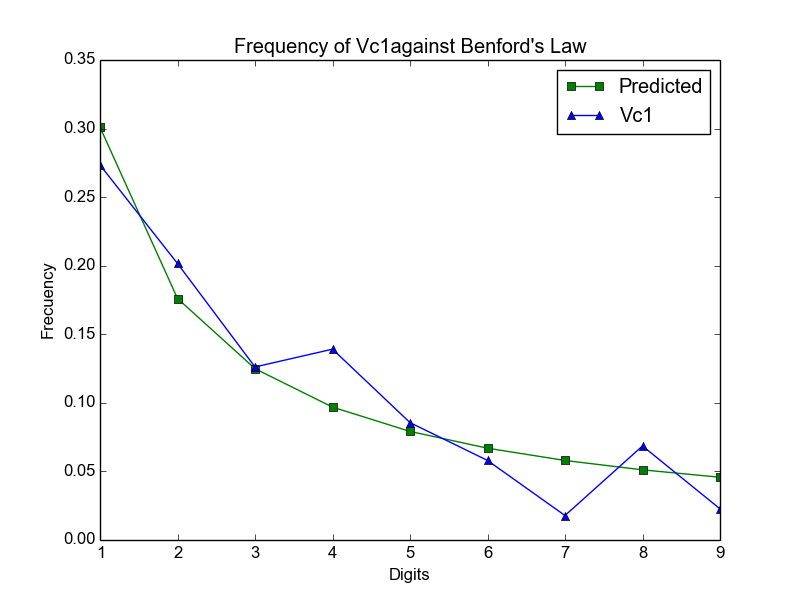
\includegraphics[scale=0.4]{imagenes/2-benford/benford_chua1775.png}
            \caption{Benford's Law against VC1}
            \end{figure}
  \item \textbf{Remarks}

We noticed that between for R between 1730 and 1775, there is a more clear First Digit Distribution according to Benford's Law, however, the measurements did not comply with MAD's Criteria which expects at most 0.015 in order to be compliant with Benford's Law. We also took a measurement with R=2000$\Omega$, value at which the system behaves as a quasi-periodic oscillator. we noticed that the first digit distribution is more uniform.

\begin{figure}
         \centering
            \begin{subfigure}[b]{0.4\textwidth}
            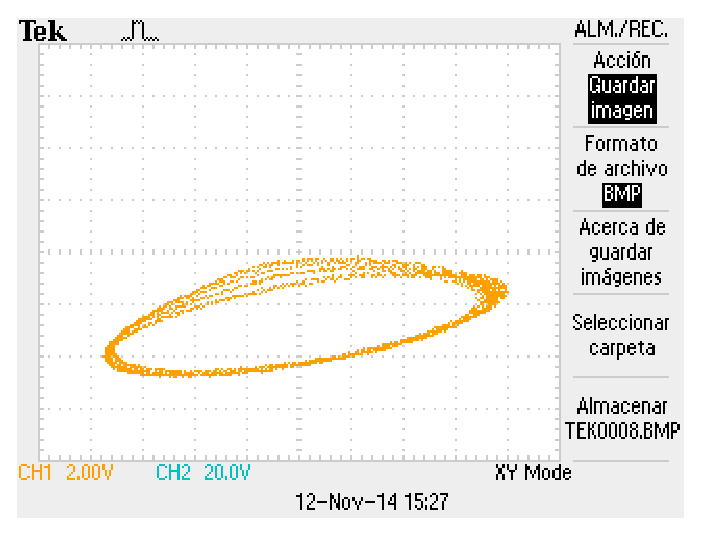
\includegraphics[width=\textwidth]{imagenes/2-benford/chua_2000.eps}
            \caption{V1-V2 $V_x$ vs $V_y$ plot}
            \end{subfigure}
            \begin{subfigure}[b]{0.8\textwidth}
            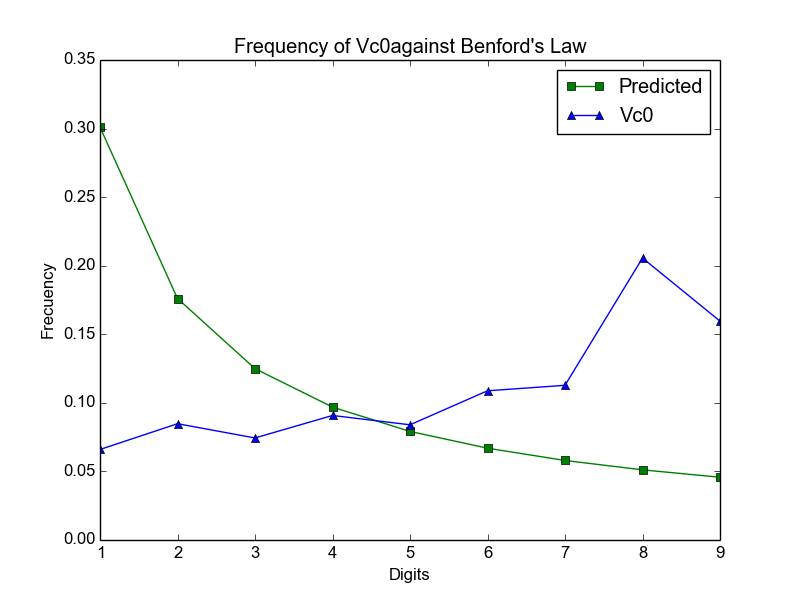
\includegraphics[width=\textwidth]{imagenes/2-benford/benford_chua20.png}
            \caption{Bifurcation Diagram varying b}
            \end{subfigure}
\end{figure}

 \end{itemize}
\subsubsection{Takougang Circuit}
 \begin{itemize}
  \item \textbf{Methodology}The circuit was connected using a standard breadboard, according to the diagram, all passive components had a nominal value equal to the ones proposed in the schematic, with a tolerance of 5\%. A regulated voltage source, set to $\pm$ 12 V was utilized to feed the active components which were the same as stated in the schematic. A third output of the regulated voltage source served to provide a stable input for the circuit ($V_b$). Next, a digital oscilloscope was used in order to obtain the data provided by the circuit.

A 1 GHz band-width oscilloscope (Agilent DSO6104A) was used next, and it was configured in order to reduce random noise. The sampler uses an averaging algorithm which delivers data with less noise, and reduces the vertical resolution (as low as 0.7 mV), with the data obtained from that oscilloscope the analysis was more reliable and results confirmed what was expected from the simulations, although only 1000 samples in an interval of 10 ms were fetched.
  \item \textbf{Results}
The first digit distribution of the voltages was taken and following the same methodology as with Chua's System, we swept through $V_b$ and took the MAD value from each distribution
\begin{center}
  \begin{tabular}{ c | c | c }
    \hline
$V_b$  & $V_x$&$V_y$\\ \hline
82mV & 0.0775279989288 & 0.0607280417648 \\ \hline
92mV & 0.0789296997697 &  0.0620760330126 \\ \hline
102mv & 0.0779822062934 & 0.0620098514762  \\ \hline
112mv & 0.0722551588234 & 0.0586329019652  \\ \hline
117mv & 0.0731369417692 & 0.0565637073089  \\ \hline
122mv & 0.0761361923841 & 0.0607646781498  \\ \hline
127mv & 0.0702382876578 & 0.0581541345311  \\ \hline
132mv & 0.0726371865346 & 0.0568562424256  \\ \hline
137mv & 0.0723923763659 & 0.0588608733569  \\ \hline
142mv & 0.0689722218274 & 0.0566979795649  \\ \hline
147mv & 0.0649140903028 & 0.0492049220995  \\ \hline
152mv & 0.0689575397758 & 0.0540809650999  \\ \hline
157mv &0.071269709088 & 0.0556102788266   \\ \hline
167mv &0.0713877270204 & 0.0546276659144  \\ \hline
187mv & 0.0642837364043 & 0.0499581746439  \\ \hline
197mv &0.0619961498144 & 0.0491763886427  \\ \hline
217mv & 0.0644054740322 & 0.0521147934116  \\ \hline
237mv & 0.0574813303354 & 0.0515391121266  \\ \hline
257mv & 0.0552768884655 & 0.0514296383228  \\ \hline
277mv & 0.0464325092508 & 0.0450451557158  \\ \hline
112mv (H-Res) &0.0126362748635 & 0.0149581584175  \\ \hline
132mv  (H-Res)& 0.0114562387312 & 0.0056682935093  \\ \hline
152mv  (H-Res)& 0.0106402668795 & 0.0143777130129  \\ \hline
172mv  (H-Res)& 0.0077090293797 & 0.0118696485616  \\ \hline
192mv  (H-Res)& 0.00801241025011 & 0.0120739312228  \\ \hline

  \end{tabular}
  \end{center}

We notice we have the best agreement with Benford's Law with $V_b=132mV$ Which gives a MAD value of 0.0056

            \begin{figure}[h]
            \centering
            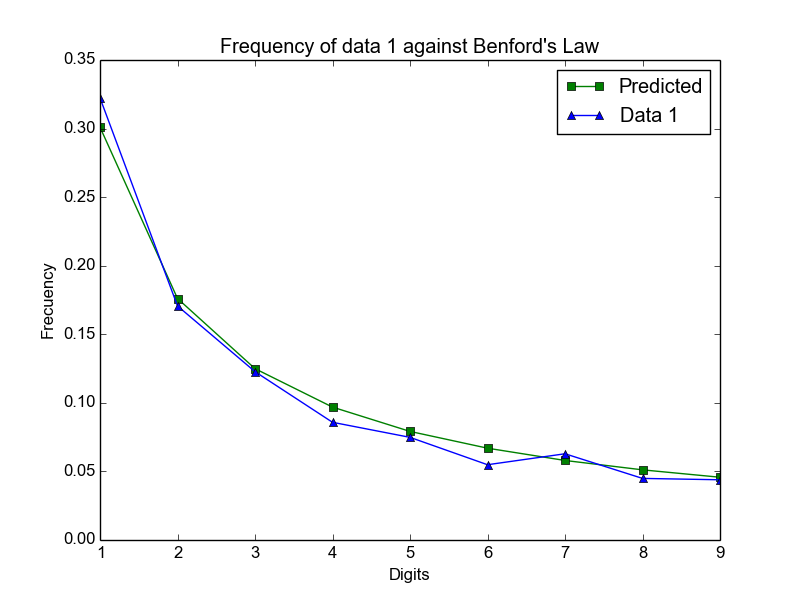
\includegraphics[scale=0.4]{imagenes/2-benford/benford_shilnikov_1.png}
            \caption{Benford's Law against digit distribution of $V_y$}
            \end{figure}

  \item \textbf{Remarks}

Simulations from Simulink gave a better accordance with $V_b=132mV$, however measuring without High-resolution sampling we did not obtain proper distributions, until we activated that sampling method, we got a distribution according to Benford's Law
 \end{itemize}


\section{Conclusion}
In the work done by Tolle \cite{Tolle00} some dynamical systems were proposed and theye checked if the first digit distribution followed Benford's Law. We took 2 autonomous circuits which displayed chaotic behaivour and verified if they were conformant according with the criterion given by Nigrini et. al. \cite{Nigrini97}. According to our experimental results, the system which best followed the distribution whas the Third Order Autonomous System proposed by Takougang et.al \cite{Takougang13}.

Verifyng the results from \cite{Takougang13}, we notice that this circuit has a Shilnikov heteroclinic orbit, which implies by the Shilnikov Criterion that the system has horseshoe chaos. This type of chaos produces time signals called chaotic bursting oscillations (see Fig. 4.1)
\begin{figure}[h]
            \centering
            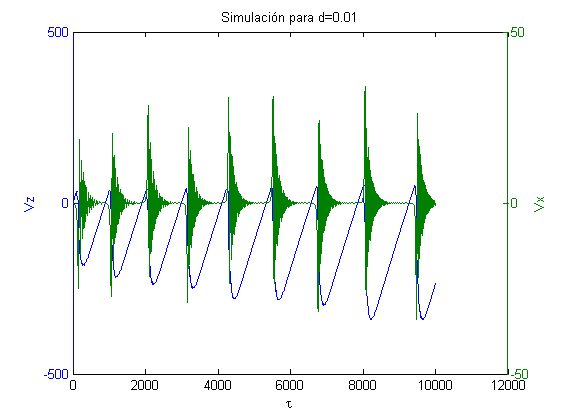
\includegraphics[scale=0.6]{imagenes/2-benford/bursting_oscilatons.png}
            \caption{$V_y$ response as a function of time}
            \end{figure}


This type of oscillations are found in biological phenomena, such as $Ca^2+$ oscillations in non-excitable cells \cite{Perc03}, pancreatic $\beta$ cells \cite{Sherman88} and in neurons\cite{Ermentrout09} and heart oscillatons, also, the work by Kreuzer et. al. \cite{Kreuzer14} indicates that brain electrical activity follows Benford's Law, so it would be interesting to see if Benford's Law could be an indicative if Real life phenomena is modelled correctly by the system if both follow Benford's Law (as it was first indicated by \cite{Tolle00}) and also to try to verify if other systems that present this kind of oscillations also follow Benford's Law.

%----------------------------------------------------------------------------------------
%  BIBLIOGRAPHY
\begin{thebibliography}{1}

\bibitem{Benford38}
  Benford Frank,
  \emph{The law of anomalous numbers}.
  Proc. Amer. Philos. Soc. 78,
  (1938),
  551-572.

\bibitem{Nigrini97}
  Nigrini Mark J., Mittermaier Linda J.
  \emph{The use of Benford's Law as an Aid in Analytical Procedures}
  Auditing: A Journal of Practice \& Theory,
  (1997),
  52-67

\bibitem{Kreuzer14}
  Matthias Kreuzer, Denis Jordan, PhD, Bernd Antkowiak, Berthold Drexler, Eberhard F. Kochs, and Gerhard Schneider
  \emph{Brain Electrical Activity Obeys Benford's Law}
  Neuroscience in Anesthesiology and Perioperative Medicine,
  (2014),
  183-191
\bibitem{Strogatz14}
 Steven H. Strogatz
  \emph{Nonlinear Dynamics and Chaos, With Applications to Physics, Biology, Chemistry and Engineering, Second Edition}
  Westview Press,
  (2014),
  309-191
\bibitem{Parlitz92}
  U. Parlitz
  \emph{Lyapunov's Exponent from Chua's Circuit}
  Journal of Circuits, Systems, and Computers,Vol. 3, No.2
  (1992),
  507-523
\bibitem{Kennedy95}
  Michale Peter Kennedy
  \emph{Experimental Chaos from Autonomous Electronic Circuits}
  Phil. Trans. R. Soc. Lond. A,
  (1995),
  507-523

\bibitem{Ayrom86}
Ayrom F.,
 \emph{Chaos in Chua's Circuit},
 IEE Proceedings, Vol. 133, No. 6 307-312
 , 1986,
 307-312


\bibitem{Takougang13}
Sifeu Takougang Kingni, Lars Keuninckx, Paul Woafo,  Guy Van der Sande, Jan Danckaert
\emph{Dissipative chaos, Shilnikov chaos and bursting oscillations
in a three-dimensional autonomous system: theory
and electronic implementation}
Nonlinear Dynamics,
2013

\bibitem{Torres07} Torres J. et al.,
 \emph{How do numbers begin? (The first digit law)},
  Eur. J. Phys., Vol. 28,
   2007,
   17-25

\bibitem{Tolle00}
Charles R. Tolle, Joanne L. Budzien, and Randall A. LaViolette
\emph{Do dynamical systems follow Benford’s law?}
Chaos: An Interdisciplinary Journal of Nonlinear Science 10,
 331,
2000
\bibitem{Perc03}
Perc, M., Marhl, M.
\emph{ Different types of bursting calcium
oscillations in non-excitable cells},
Chaos Solitons Fractals 18,
 759–773
2003
\bibitem{Sherman88}
Sherman, A., Rinzel, J., Keizer, J.
\emph{ Emergence of organized bursting in clusters of pancreatic $\beta$-cells by channel sharing},
Biophys. J. 54, 411–425,
1988
\bibitem{Ermentrout09}
\emph{Mathematical Foundations of Neuroscience}
Interdiscplinary Applied Mathematics 35,
103-126,
2009
\end{thebibliography}

% \end{document}


    \chapter{Dinámica de vuelo del Boomerang: modelo, simulación y obtención de información de vuelo mediante un sensor embarcado}
    \paragraph{Néstor Abraham Aguillón Balderas, Carlos Antonio Tovar García}
    % \input{estilo/completo.tex}
%
% \begin{document}
%
%     \clearpage
%     
    \setlength{\unitlength}{1 cm} %Especificar unidad de trabajo
    \thispagestyle{empty}
    \begin{picture}(18,4)
    \put(0,0){
\includegraphics[width=3cm,height=4cm]{imagenes/cinvestav.jpg}}
    \end{picture}
    \\
    \\
    \begin{center}
    \textbf{{\LARGE Centro de Investigación y de Estudios Avanzados del IPN}}\\[1cm]
    {\LARGE Departamento de Control Automático}\\[1.25cm]
    {\Large Modelado y Simulación de Sistemas}\\[2.3cm]
    {\LARGE \textbf{Dinámica de vuelo del Boomerang: modelo, simulación y obtención de información de vuelo mediante un sensor embarcado}}\\[2cm]
    {\large Néstor Abraham Aguillón Balderas}\\[0.5cm]
    {\large Carlos Antonio Tovar García}\\[2cm]
    México, Distrito Federal - \today
    \end{center}

    \section*{Resumen} 

	El boomerang es un artefacto conocido mundialmente por el interesante comportamiento que presenta al ser arojado correctamente. Su comportamiento durante el vuelo es explicado por la interacción de sus alas en movimiento con el viento, lo cual genera efectos de precesión y recostamiento. Algunas variables de las ecuaciones dinámicas necesitan ser suavizadas o promediadas para simplificar su solución por medio de un método de integración numérica. Un simulador y su interfaz gráfica fueron desarrolladas a partir de estas ecuaciones simplificadas en $Matlab_{\textregistered}$. Finalmente se llevaron a cabo experimentos con un sensor de medición inercial embarcado en un boomerang con el objetivo de recopilar datos para la futura reconstrucción de la trayectoria de vuelo.

\begingroup
\let\clearpage\relax

\section*{Abstract}


	A boomerang is an artifact known worldwide for its interesting behavior when thrown correctly. His behavior during flight can be explained by the interaction of its moving wings with the air, generating effects such as precession and lying down. Some variables of the dynamic equations need to be smoothed or averaged in order to simplify their solutions throught a numerical integration method. A simulator and its graphical interface were developed from these simplified equations in $Matlab_{\textregistered}$. Finally, some experiments were performed using an inertial measurement unit mounted on a boomerang for the future reconstruction of the flying path.

\endgroup


    % \clearpage
    % \tableofcontents
\listoffigures
%\listoftables


    \section{Introducción}

	El estudio de la dinámica del vuelo del boomerang no resulta ser un trabajo científico nuevo, por lo que existen pocos especialistas interesandos en resolver esta problemática. Pero resulta de gran curiosidad explicar la razón de su vuelo a toda persna que lo haya visto volar.

	La investigación acerca del comportamiento de un boomerang no resulta ser estudio de la ciencia moderna, sino más bien un trabajo de varias generaciones. Algunos métodos utilizados para este comportamiento estan basados en la aerodinámica y la hidrodinámica.  \cite{Hess1975}.

		A continuación se presenta una breve introducción sobre el origen de los boomerangs, dos tipos de estos y los objetivos del documento:

\subsection{Origen del Boomerang}

	Como es bien conocido, los boomerangs son usados y manufacturados principalmente por los aborigenes de Australia. El término $"boomerang"$ es vagamente definido como: un objeto de madera que, al ser lanzado de una manera apropiada, por su interacción con el aire, atraviesan una trayectoria de vuelo que va de regreso a una vecindad del punto de lanzamiento. Cabe descatar que gran porcentaje de los boomerangs Australianos no son diseñados para regresar sino más bien para cazar ó como arma, por lo que los que son capaces de regresar son usados para diversión. \cite{Hess1975}

	Cuando los primeros Europeos llegarón a Austrialia los boomerangs ya estaban ahí. Cuando Dampier visitó la costa occidental de Australía en 1688 hizo la primera mención de ellos: \textit{Algulos Australianos tienen espadas de maderas, otros tienen una especie de lanzas. Las espadas son una pieza de madera formadas como un chafarote (Cuchillo de gran tamaño, corto y ancho)}. \cite{Dampier1729}

	Los boomerang aborígenes australianos más antiguos, datan aproximadamente de 9000 años de antigüedad, pero palos de caza más antiguos han sido descubiertas en Europa, donde parece que han formado parte de la edad de piedra arsenal de armas. Un boomerang que fue descubierto en Jaskinia Oblazowa en las montañas de los Cárpatos en Polonia era de colmillo de mamut y se cree que tienen cerca de 30.000 años de antigüedad. El Rey Tutankamón,  famoso faraón del antiguo Egipto que murió hace más de 3000 años, era propietario de una colección de boomerangs. \cite{Lorenz}

\subsection{Tipos de boomerangs}

  \subsubsection*{Boomerangs tradicionales}

	Esta es una arma única y curiosa, provienen principalmente de Australia. Los cuales en su mayoría no regresan al lanzador, pueden volar más o menos en línea recta por grandes distancias (140 m aprox.), y así golpear a un objeto, presa ó enemigo con una fuerza increíble . Sólo un pequeño porcentaje de los manufacturados en Australia son de regreso al lanzador.

	\begin{figure}[h]
		\begin{center}
		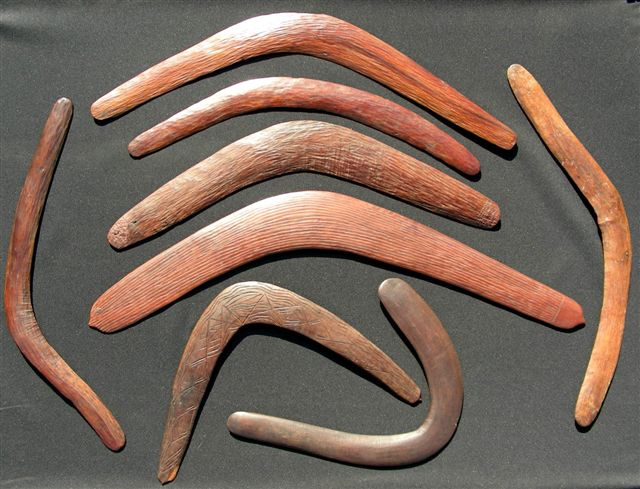
\includegraphics[scale=1]{imagenes/3-boomerang/boomerang_formas.jpg}
		\caption{Boomerangs de retorno.}
   	    \label{fig1}
		\end{center}
	\end{figure}


	Los boomerangs tradicionales son suavenmente convexos de un lado y casi planos del otro. Tienen alrededor de 6mm a 1 cm de grosor, de 5 a 7.5 cm de ancho, se extrecha hacía los extremos los cuales suelen estar redondeados ó punteados, el borde esta afilado por todas partes y la longitud varia desde 40 hasta 1 metro de longitud.

	\begin{figure}[h]
		\begin{center}
		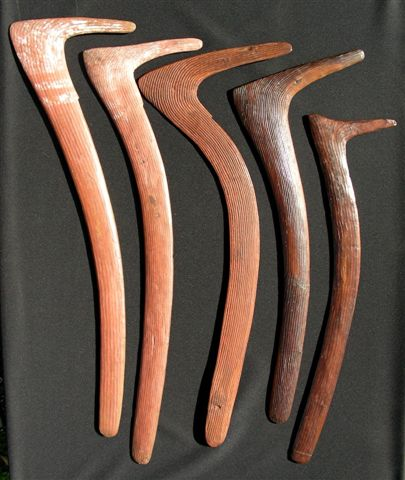
\includegraphics[scale=1]{imagenes/3-boomerang/boomerang_de_no_regreso.jpg}
		\caption{Boomerangs de no retorno.}
   	    \label{fig1}
		\end{center}
	\end{figure}

	Como se mencionó antes los boomerangs pueden ser de retorno y de no retorno, por lo que en este documento se estudian principalmente los de retorno, en particular, los llamados de 4 palas o en forma de cruz.

  \subsubsection*{Boomerangs de 4 palas}

  	Los boomerangs en forma de cruz están formadas for 4 palas de madera, las cuales tienen la misma forma que las palas de los boomerangs tradicionales.  Cada pala de tiene un tamaño de entre 20 y 30 cm de longitud y de 4 a 6 cm de ancho.

	Estos modelos también son llamados $"Cross Boomerangs"$ mostrados en la figura (\ref{fig1}), donde claramente puede notarse que difiere de los modelos tradicionales \cite{kuleshov}.
	\begin{figure}[h]
		\begin{center}
		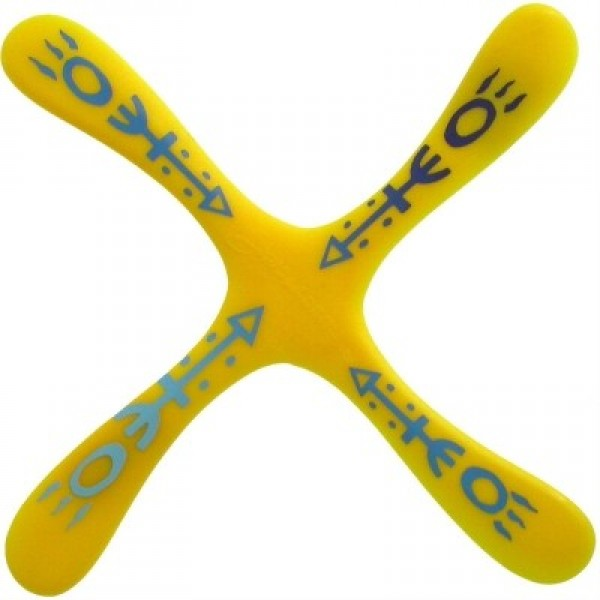
\includegraphics[scale=0.2]{imagenes/3-boomerang/boomerang4palas.jpg}
		\caption{Boomerang de 4 palas.}
   	    \label{fig1}
		\end{center}
	\end{figure}

	Para el análisis de los boomerang de 4 palas las ecuaciones de movimiento se siplifican considerablemente si consideramos que el centro de masa coincide con el punto de unión de las palas \cite{barger1973}.

	\subsection{Objetivos}

	\begin{enumerate}
	\item Modelo dinámico no lineal que describe la
	trayectoria tridimensional del boomerang en
	vuelo, a partir del lanzamiento inicial.

	\item Uso como soporte para la concepción de
	simulador computacional que describa la
	trayectoria tridimensional del boomerang.

	\item Captura de información paramétrica en vuelo
	mediante el uso de una Unidad de Medición
	Inercial miniaturizada embarcada: seguimiento de trayectoria en
	almacenamiento de datos y posterior despliegue en sistema informático.
	\end{enumerate}

	En el capítulo 1 se mostró una breve introducción sobre los boomerags, sus origenes y los objetivos generales a cubrir del proyecto. En el capítulo 2 se derivan las ecuaciones de movimiento del boomerang, así como las fuerzas que actúan sobre este y la consideración de la influencia del viento. En el capítulo 3 se presenta el simulador realizado para generar la trayectoria de vuelo del boomerang. En el capítulo 4 se presentan los experimentos y resultados obtenidos durante el desarrollo del proyecto.


    \section{Marco Teórico}

	En este capítulo primeramente se explica que características presenta un boomerang durante su vuelo para que este sea capaz de regresar al lanzador. Se derivan las ecuaciones de movimiento del boomerang y como estás pueden ser integradas fácilmente para obtener la trayectoria de vuelo, los efectos de la gravedad actuando sobre el boomerang son considerados, además se muestra como se agregan los efectos del viento en las ecuaciones de movimiento.

	\subsection{Boomerangs desde un punto de vista físico}

	En esta sección se tratarán conceptos y fenómenos relacionados con el funcionamiento básico del boomerang, los cuales permitirán comprender de manera general la física asosiada a este.

		\subsubsection{Comportamiento de boomerangs de retorno}

	Recordando el concepto, los boomerangs son objetos que, al ser lanzados apropiadamente, vuelan girando rapidamente a través del aire y regresan cerca del punto de lanzamiento \cite{Hess1975} (en este documento no se considerarán los boomerangs de no retorno).

	Un boomerang de retorno (diestro) típico es lanzado en plano vertical (o ligeramente inclinado con su parte superior alejada del lanzador); en dirección horizontal (o ligeramente elevada); y con giro considerable. Al inicio, la trayectoria del boomerang sigue la dirección del vector de velocidad inicial aplicado, pero pronto presenta un desvío a la izquierda y hacia arriba, traza un bucle amplio, se acerca al lanzador y puede descender en algún lugar cerca de los pies de este, o describir un bucle más pequeño antes de tocar el suelo. Generalmente, el plano de rotación del boomerang se ``acuesta'' gradualmente de tal manera que puede estar horizontal al final del vuelo.

		\subsubsection{Lanzamiento}

	Los boomerangs de retorno pueden tener diversas formas, pero siempre consisten en dos o más brazos descansando aproximadamente en un plano. Una caracteristica escencial es la sección transversal de cada brazo, la cual es mas convexa en un lado que en otro.

	Un boomerang es lanzado sujetandolo de uno de sus extremos con el lado más convexo cerca  de la mejilla del lanzador y arrojandolo hacia adelante de manera que es liberado con un giro rápido respecto a su centro de masa (perpendicular al plano de lanzamiento).

			\begin{figure}[ht]
			\begin{center}
			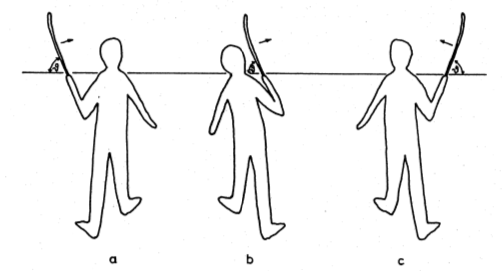
\includegraphics[scale=0.5]{imagenes/3-boomerang/Lanzamiento.png}
			\caption{Vista trasera de un lanzador (Tomada de \cite{Hess1975}).}
			\label{fig1}
			\end{center}
			\end{figure}

	En la Fig. \ref{fig1} se puede observar el ángulo $\vartheta$, es cual es el ángulo entre el boomerang y la horizontal y destacan tres tipos de lanzamientos:

		\begin{enumerate}[a)]
		\item Lanzador zurdo lanzando un boomerang zurdo,
		\item Lanzador diestro lanzando boomernag zurdo y
		\item Lanzador diestro lanzando boomerang diestro.
    	\end{enumerate}

	El ángulo $\vartheta$  entre el plano de lanzamiento del boomerang y el horizonte (vease la Fig. \ref{fig1}) tiene gran influencia en la trayectoria de vuelo. La mayoría de los boomernangs deben ser lanzados con un ángulo $\vartheta$  de entre 45 y 90 grados. Si un boomerang es lanzado a ángulos menores, generalmente describe una trayectoria ascendente y finalmente cae al suelo a gran velocidad.

		\subsection{ Los principios del boomerang de retorno}

	Aquí se presenta un modelo elemental del funcionamiento del boomerang de retorno.

	Una característica escencial del boomerang es la forma de la sección transversal de sus brazo (o aspa). Estas tienen forma de ala de avión (o de ave). Si un aeroplano vuela horizontalmente a través del aire, su peso debe ser contrarrestado por una fuerza de empuje que lo sostenga, o de otra manera caería al suelo. Esta fuerza surge de la interacción del viento con las alas del avión.

		\begin{figure}[ht]
		\begin{center}
		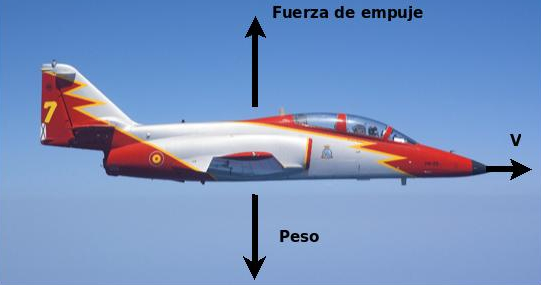
\includegraphics[scale=0.4]{imagenes/3-boomerang/plane.jpg}
		\caption{Aeroplano volando horizontalmente a velocidad V. El peso es cotrarrestado por una fuerza aerodinámica de empuje.}
		\label{fig2}
		\end{center}
		\end{figure}

	Las alas del boomerang, como las del avión tienen una forma especial que produce fuerzas aerodinámicas casi perpendiculares a la dirección de estas.

	Recuerdese que se mencionó que el brazo del boomerang presenta una cara más convexa que la otra  (lo cual es también el mismo caso de los aviones).

	La interacción del aire con la sección más convexa genera una presión del aire más baja que la producida por su contra parte. La diferencia de presiones produce una fuerza resultante de empuje, como se puede ver en la Fig. \ref{fig3}.a. Además, si el ala es inclinada más y más, la fuerza resultante se vuelve más grande Fig. \ref{fig3}.b.

		\begin{figure}[ht]
		\begin{center}
		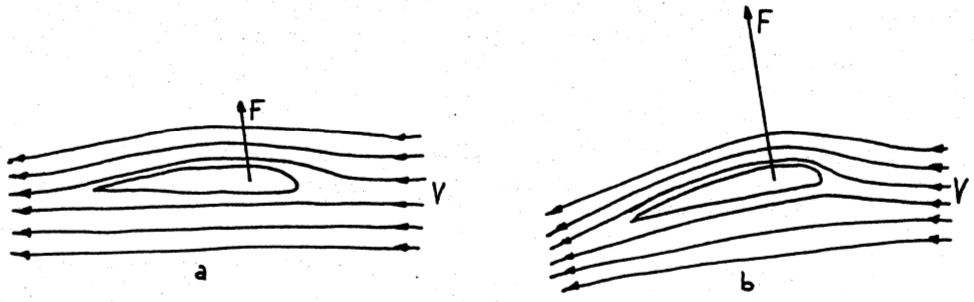
\includegraphics[scale=0.3]{imagenes/3-boomerang/airFlow.png}
		\caption{Flujo de aire alrededor de ala. F es la fuerza resultante. a: Sin inclinación aparente. b: con inclinación adicional.}
		\label{fig3}
		\end{center}
		\end{figure}
\newpage
    Recordemos que un boomerang de retorno diestro es lanzado usualmente de tal manera que su plano de rotación es casi vertical con el lado más convexo hacia la izquierda. Por tanto se produce una fuerza de empuje del lado menos convexo al más convexo, es decir, hacia la izquierda (Fig. \ref{fig4}), la cual acelera al boomerang en dicha dirección.\\\\

		\begin{figure}[ht]
		\begin{center}
		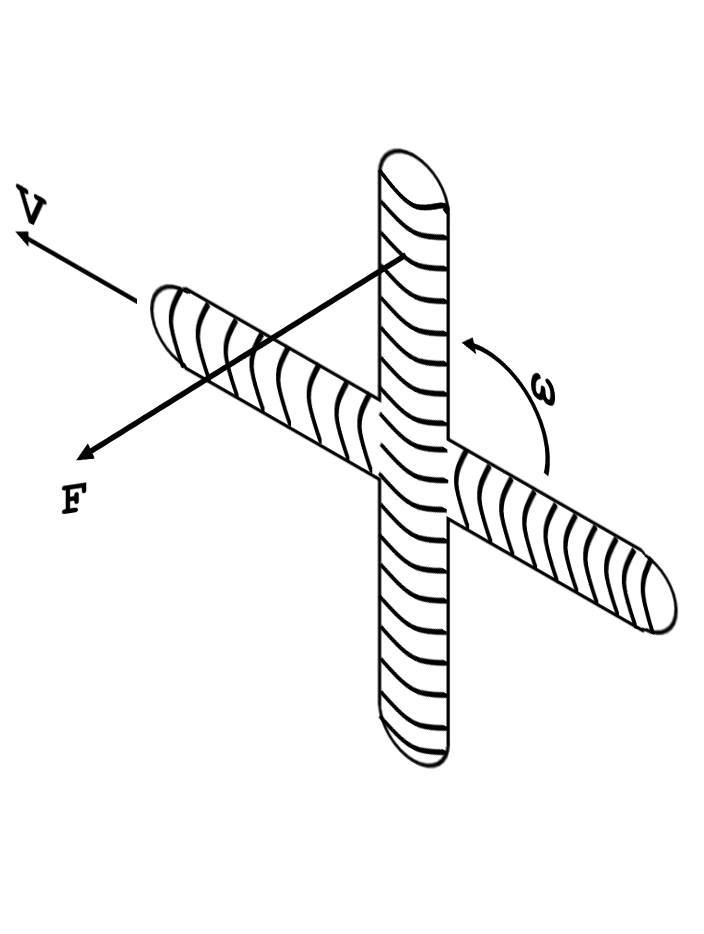
\includegraphics[scale=0.25]{imagenes/3-boomerang/leftwardForce.png}
		\caption{Fuerza resultante hacia la izquierda para boomerang diestro.}
		\label{fig4}
		\end{center}
		\end{figure}

	En adelante, particularizaremos por conveniencia a boomerangs diestros de cuatro palas (brazos). El centro de masa (CM) se encuentra en el punto de unión de sus cuatro alas y la distancia de este a cada una de las puntas es a. Se presenta una velocidad de avance $(V)$ y una velocidad angular $(\omega)$. A cada instante, no todas las particulas del boomerang tienen la misma velocidad, lo cual es resultado de la combinación de V y w.

		\begin{figure}[ht]
		\begin{center}
		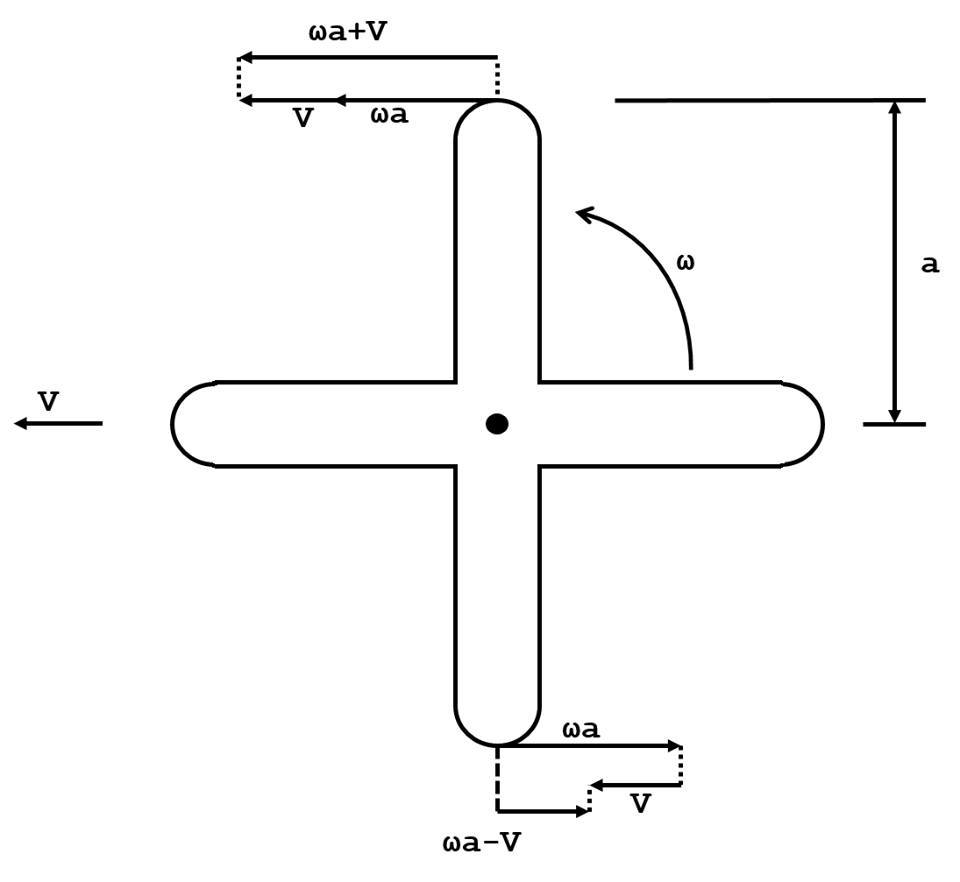
\includegraphics[scale=0.205]{imagenes/3-boomerang/upwardPointingEndofBoomerang.png}
		\caption{Velocidad de avance en los extremos superior e inferior del boomerang.}
		\label{fig5}
		\end{center}
		\end{figure}

	La punta superior del boomerang se mueve más rapido que la inferior debido a que en la primera tenemos una velocidad $V+wa$ y en la segunda tenemos $V-wa$. Generalizando tenemos que toda particula superior presenta una fuerza mayor de empuje hacia la izquierda del plano de rotación que cualquier inferior. Por lo tanto, las fuerzas aerodinamicas no solo producen una fuerza neta , sino también un par T que trata de inclinar el boomerang por su parte superior hacia la izquierda (Fig. \ref{fig6}). Esta inclinación seria respecto a un eje horizontal imaginario, llamado eje de torción, sin embargo, dicha torción no se aprecia en un boomerang.

		\begin{figure}[ht]
		\begin{center}
		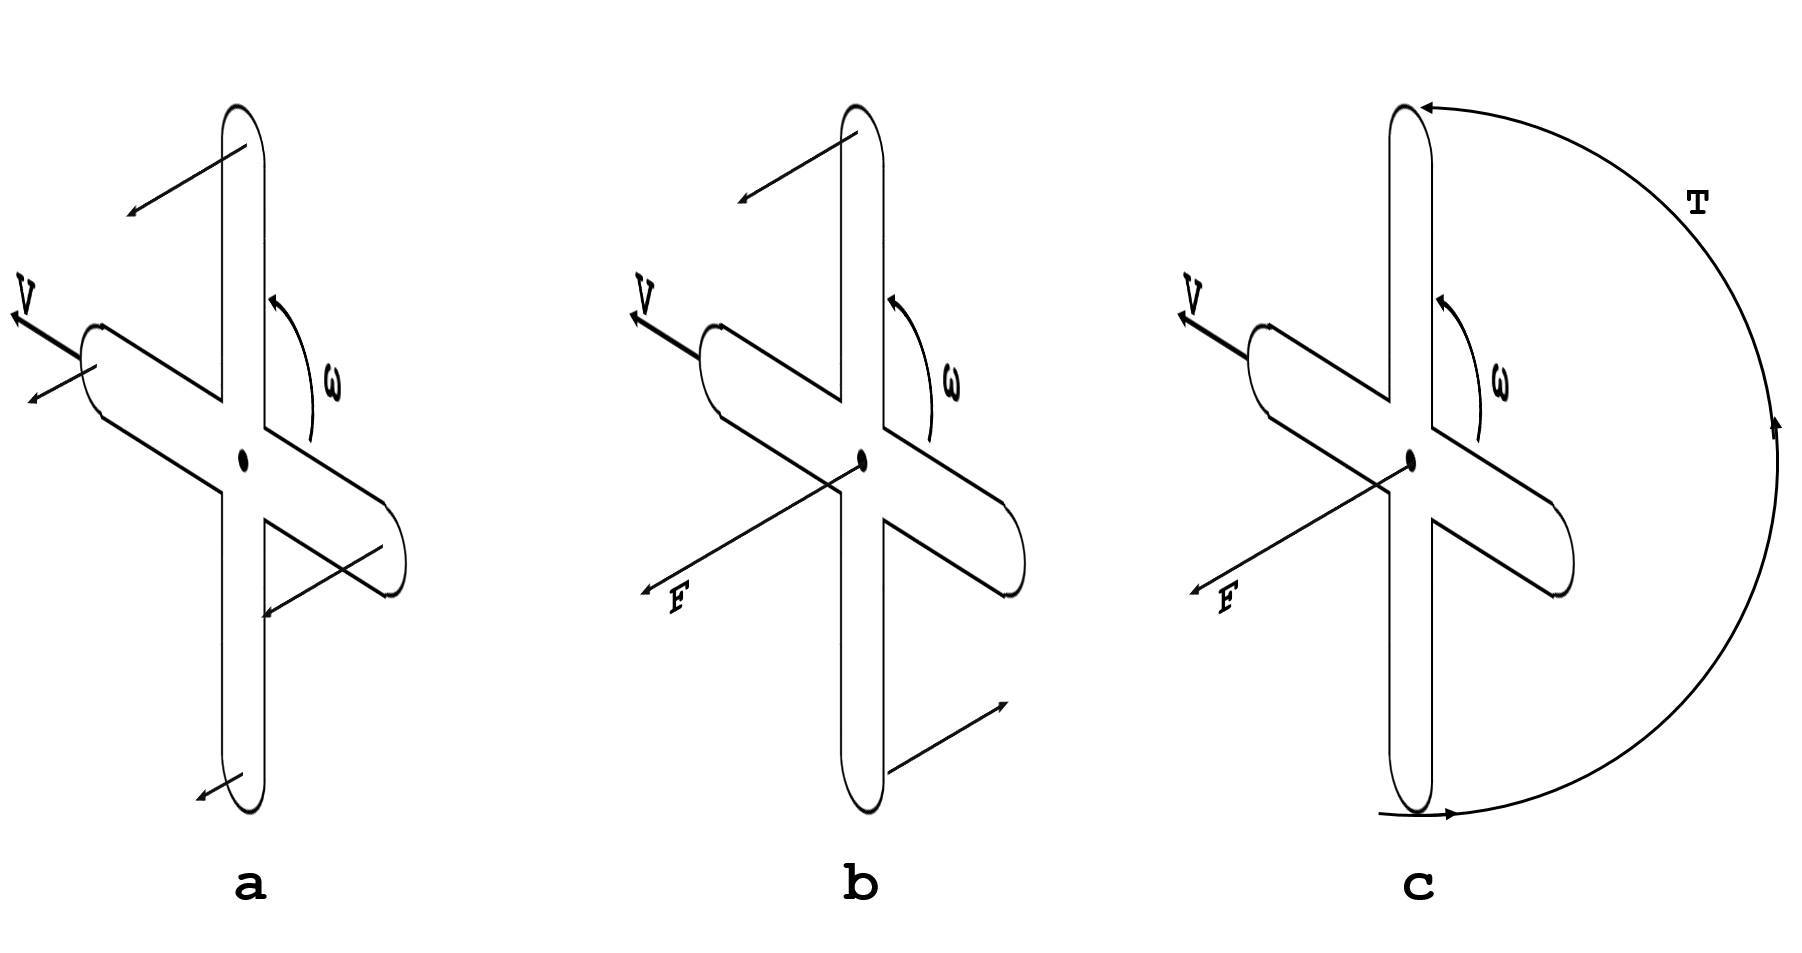
\includegraphics[scale=0.15]{imagenes/3-boomerang/DistrutionOfLEftwardForces.png}
		\caption{a: Distribución de fuerzas izquierdas. b: Fuerzas equivalentes actuando en el centro y los extremos superior e inferior del boomerang. c: Las fuerzas forman un par T, el cual trata de rotar el boomerang de su parte superior hacia la izquierda.}
		\label{fig6}
		\end{center}
		\end{figure}
\newpage
	Ahora introduciremos el concepto de movimiento de precesión:

	Pon un trompo sobre su punta y logicamente caera, pero inducele un giro rápido y se mantendra en pie. Un trompo en rotación reacciona de una manera peculiar a un par aplicado: No cede al par, en cambio rota despacio respecto a un eje imaginario perpendicular a los ejes de rotación y torción \cite{Hess1975}. Este efecto se define como ``movimiento de precesión''.

	Debido a la combinación del par generado por las fuerzas aerodinámicas y su rápida rotación, el boomerang presenta un movimiento de precesión respecto a un eje imaginario perpendicular a los ejes de rotación y de torsión.

	Si se considera un boomerang diestro al inicio del vuelo, su eje de rotación es horizontal hacia la izquierda y el eje de torsión horizontal hacia atras, por tanto, este rota (con una velocidad angular $\omega$) hacia la izquierda su parte delantera en lugar de la superior debido al efecto de precesión (Vease Fig. \ref{fig7}).

		\begin{figure}[ht]
		\begin{center}
		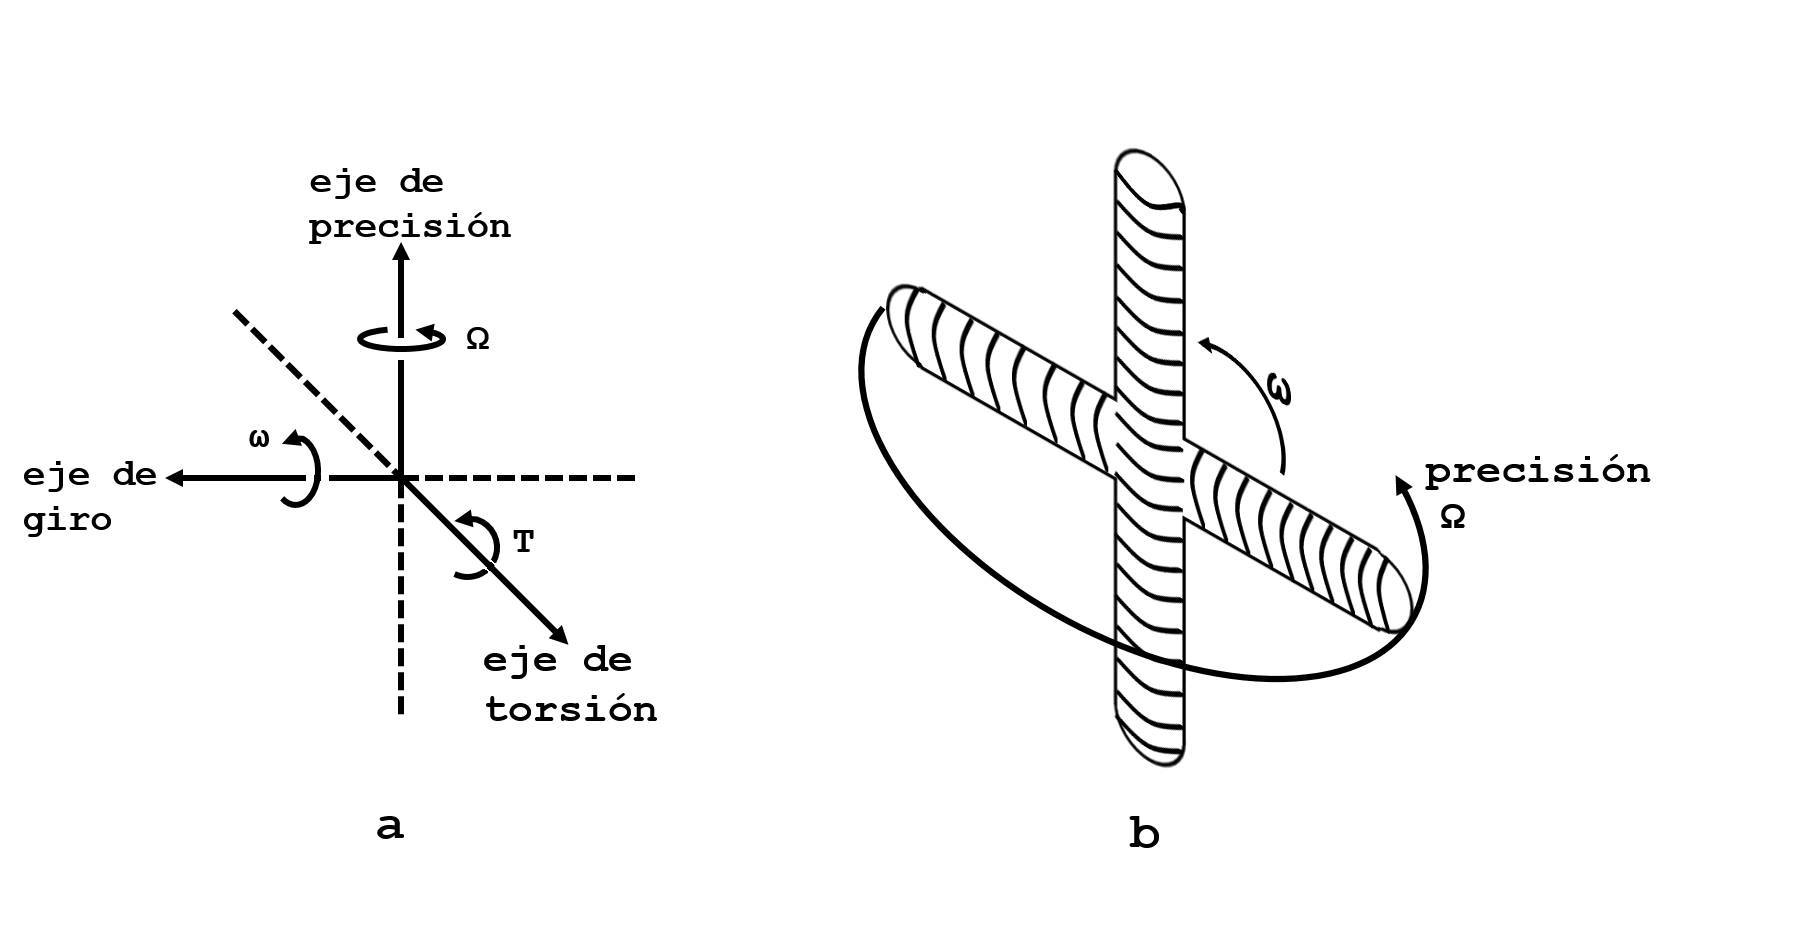
\includegraphics[scale=0.25]{imagenes/3-boomerang/precesionAlrededorDeOmega.png}
		\caption{a) Precesión $\Omega$ con respecto a un eje perpendicular a al eje de torción y el eje de rotación. b) Precesión del boomerang.}
		\label{fig7}
		\end{center}
		\end{figure}

	Para entender mejor el efecto de precesión, observese la Fig. \ref{fig8}. Podemos descartar la fuerza neta resultante en el centro de masa debido a que su único efecto es acelerar el boomerang hacia la izquierda. El par T es originado por las fuerzas de la parte superior e inferior, de igual magnitud y con sentido opuesto (vease Fig. \ref{fig5}). La maxima fuerza izquierda es ejercida por la punta superior (Fig. \ref{fig8}.a), la cual es acelerada gradualmente hasta alcanzar una velocidad, la cual alcanza su valor máximo cuando este punto se convierte en la punta frontal (Fig. \ref{fig8}.b). Cuando esta parte desciende más, el par T empieza a empujarla hacia la derecha, lo cual decrementa su velocidad. La fuerza derecha máxima se presenta cuando la punta considerada está en el punto más bajo (Fig. \ref{fig8}.c), donde la velocidad izquierda ha desaparecido y la velocidad derecha comienza a crecer, alcanzando su punto máximo a mitad del camino al punto superior (Fig. \ref{fig8}.d), y se desvanec al completar una revolución (Fig. \ref{fig8}.a). El resultado de esta secuencia es indicado en la Fig. \ref{fig8}.e.


	La combinación de velocidad hacia la izquierda en la parte frontal y velocidad hacia derecha en la parte posterior constituye el movimiento de precesión, es decir, el boomerang rota su plano respecto a un eje imaginario vertical. A mayor par, una precesión más rápida.

		\begin{figure}[ht]
		\begin{center}
		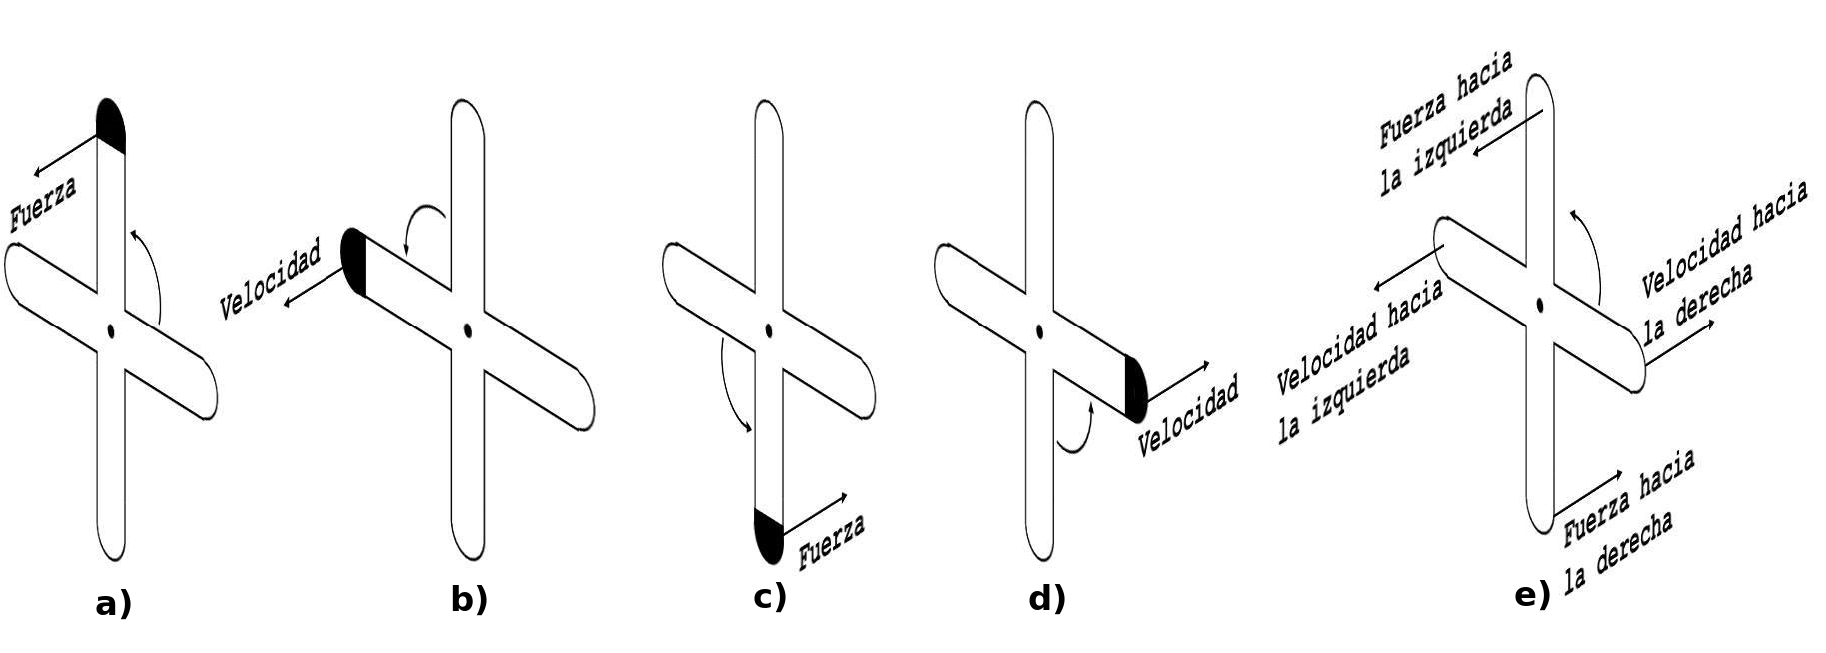
\includegraphics[scale=0.15]{imagenes/3-boomerang/PrecesionDelBoomerang.png}
		\caption{Precesión del boomerang. a,b,c,d: puntas del boomerang durante el transcurso de la revolución. e: La parte frontal tiene una velocidad hacia la izquierda, y la parte posterior hacia la derecha.}
		\label{fig8}
		\end{center}
		\end{figure}

	Ahora llamemos $\Psi$ al angulo entre el plano de rotación del boomerang y la dirección de su velocidad de avance V. Si $\Psi$ = 0, el boomerang se mueve paralelo a su propio plano de rotación. Si $\Psi>0$, el boomerang esta inclinado con respecto a la dirección de movimiento y las fuerzas aerodinamicas son mayores ya que las alas estaran inclinadas también y experimentara un empuje mayor (vease Fig. \ref{fig3}).\\

	Consideremos tres casos hipoteticos indicados esquematicamente en la Fig. \ref{fig9}.

		\begin{figure}[ht]
		\begin{center}
		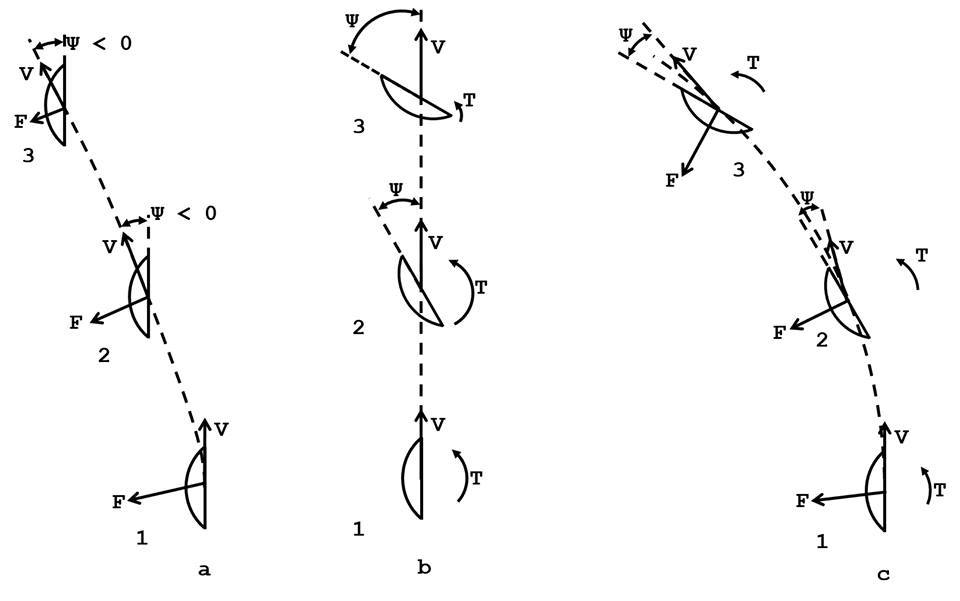
\includegraphics[scale=0.3]{imagenes/3-boomerang/TresCasos.png}
		\caption{a) Solo la fuerza F actúa. b) Solo el par T actúa. c) Actua el par T y la fuerza F. V es la velocidad de avance. $\Psi$ es el ángulo de incidencia. 1,2,3: posiciones sucesivas en vista superior.}
		\label{fig9}
		\end{center}
		\end{figure}

	Caso a: Solo la fuerza neta F actúa, el par neto T es despreciable. El boomerang adquiere una velocidad hacia la izquierda, adicional a su velocidad de avance original. Su plano de rotación permanece paralelo a si mismo. Esto resulta en un angulo de incidencia cada vez más negativo: $\Psi$<0. Conforme esto sucede, la fuerza F decrece hasta que se desvanece y el boomerang finalmente vuela en linea recta a una $\Psi$ constante menor a cero.

	Caso b: Solo el par neto T actua, la fuerza neta F es despreciable. El boomerang vuela en linea recta a velocidad constante.  Mientras tanto, la precesión rota al boomerang en contra de las manecillas del reloj respecto a un eje imaginario perpendicular al suelo. Esto incrementa el ángulo de incidencia $\Psi$ cada vez más. Si T no se desvanece antes de que $\Psi$ sea igual a 90 grados, el boomerang finalmente se moverá perpendicular a su trayectoria de vuelo.

	Caso c: Actua tanto el par T como la fuerza F. En un buen boomerang, estos efectos están balanceados. Si el par T causa un incremento de $\Psi$, la fuerza F también incrementará, empujando el boomerang hacia la izquierda, restringiendo el incremento excesivo de $\Psi$. El resultado es una trayectoria de vuelo curva.

	Si el boomerang se mueve en un plano no vertical, es decir, con un ángulo menor a 90 grados respecto a un eje imaginario del CM hacia su parte posterior, la fuerza F puede tener una componente hacia arriba que contrarreste el peso y mantenga al boomerang en el aire por más tiempo.

	Por otro lado, es posible inclinar una ala de cualquier sección transversal en un ángulo, denotado por ``ángulo de ataque'', tal que la fuerza de empuje resultante sea cero (Fig. \ref{fig10}.a) presentando solo un poco de arrastre. Para una sección transversal plana esta dirección es obviamente paralela al plano del ala. Para alas con un lado más convexo en la parte superior esta sección corresponde a una inclinación aparentemente negativa. A cualquier otro ángulo de ataque, el ala va a generar fuerza de empuje (vease Fig. \ref{fig10}.b). El ángulo ($\alpha$) entre la inclinación de empuje cero y la inclinación actual es llamada ``sección de angulo de ataque efectivo''. Si este ángulo $\alpha$ es suficientemente pequeño (digase $|\alpha| <= 10 grados$), el empuje es aproximadamente proporcional a este.

		\begin{figure}[ht]
		\begin{center}
		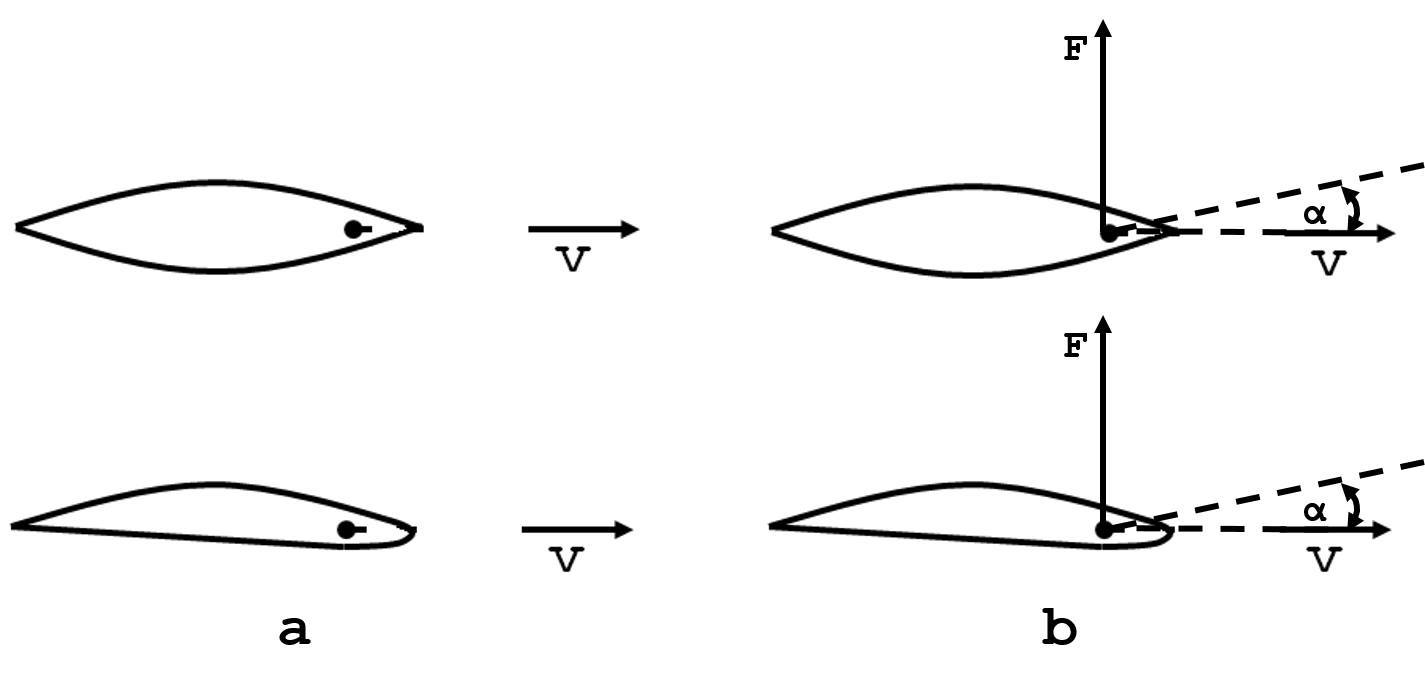
\includegraphics[scale=0.2]{imagenes/3-boomerang/atackangle.jpg}
		\caption{Ángulo de ataque.}
		\label{fig10}
		\end{center}
		\end{figure}

		\subsection{Más de la mecánica del boomerang.}

	En esta sección trataremos dos temas:
    	\begin{enumerate}[A)]
		\item El tamaño de la trayectoria del booerang.
		\item El recostamiento del boomerang.
		\end{enumerate}

	A: El tamaño de la trayectoria del boomerang.

	Supongase que un boomerang vuela aproximadamente a lo largo de un círculo horizontal, con su plano de rotación vertical, y con un ángulo de incidencia $\Psi$ pequeño y constante. Sea la velocidad de avance V ($\frac{m}{s}$) y su velocidad angular $\omega$ ($\frac{rad}{s}$). Sea una velocidad de precesión $\Omega$ ($\frac{rad}{s}$) relacionada con el par T y w de acuerdo con la formula:

		\begin{equation}
		\Omega = \frac{T}{I\omega}
		\label{ec1}
		\end{equation}  %% 17.1


	donde I es el momento de inercia del objeto respecto a su eje de rotación.

		\begin{figure}[ht]
		\begin{center}
		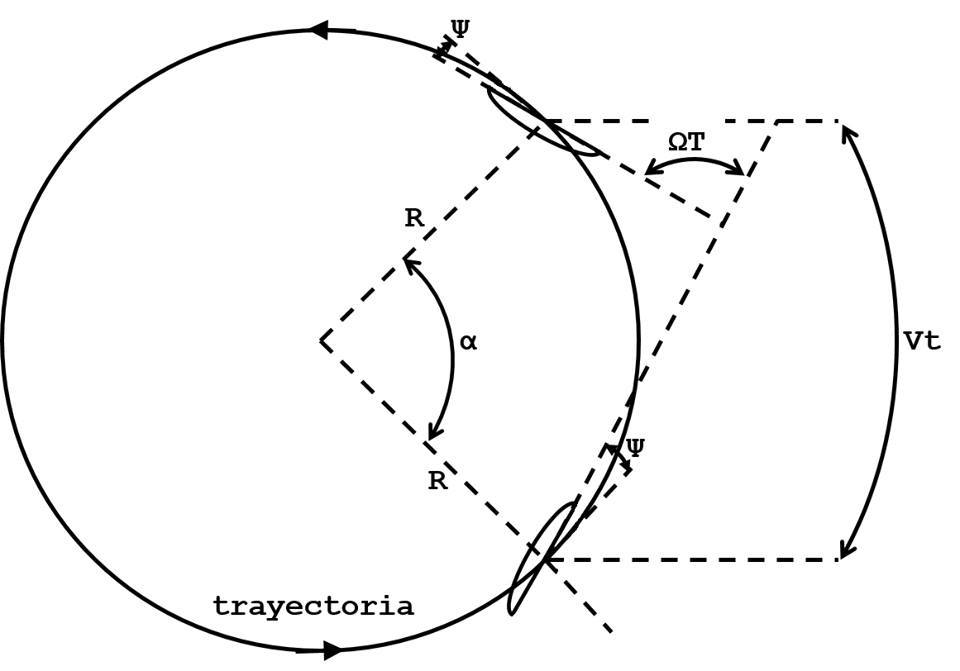
\includegraphics[scale=0.3]{imagenes/3-boomerang/TrayectoriaCircular.png}
		\caption{Posición del boomerang en dos instantes, con t segundos de separación (vista superior).}
		\label{fig11}
		\end{center}
		\end{figure}


	Sea R el radio de la trayectoria circular (vease Fig. \ref{fig11}). En un tiempo t, el boomerang describe un arco de longitud $Vt$ metros. El ángulo, visto desde el centro de la trayectoria se denota como $\alpha$, de tal manera que la longitud del arco es $\alpha R$. Por tanto: $\alpha R = Vt$. En el mismo intervalo de tiempo, el boomeran realiza un movimiento de precesión generando un ángulo de $\Omega t$. Si el ángulo de incidencia $\Psi$ (angulo entre el plano del boomerang y la trayectoria de vuelo) es constante, tenemos que $\Omega T = \alpha$. Entonces $\Omega t R = V t$ y

		\begin{equation}
		\Omega R = V
		\label{ec2}
		\end{equation} %% 17.2

	Para hacer volar un boomerang a lo largo de una trayectoria curva de radio R, una fuerza centrípeta (dirigida hacia el centro del círculo) es requerida de magnitud $\frac{m V^{2}}{R}$, donde m es la masa del boomerang. Esta fuerza, por supuesto, es suprimida por la fuerza aerodinámica F, por tanto

		\begin{equation}
		F = \frac{m V^{2}}{R}
		\label{ec3}
		\end{equation} %% 17.4

	Para el radio R de la trayectoria de vuelo obtenemos

		\begin{equation}
		R = \frac{mV^{2}}{F}
		\label{ec4}
		\end{equation} %% 17.4

	Además, de (17.1) y (17.2) tenemos que

		\begin{equation}
		R = \frac{V}{Omega} = \frac{IwV}{T}
		\label{ec5}
		\end{equation} %% 17.5

	De (17.4) y (17.5) se obtiene la condición

		\begin{equation}
		\frac{T}{Iw} = \frac{F}{mV}
		\label{ec6}
		\end{equation} %% 17.6

	Ambos T $\&$ F dependen del ángulo de incidencia $\Psi$. Por tanto, $\Psi$ tiene un valor tal que (\ref{ec6}) se satisface. Enfatizamos, sin embargo, que este forma de vuelo no siempre es posible.

	Consideremos ahora el caso en que el boomerang es arrojado a una velocidad mayor, de tal manera que V y $\omega$ incrementan. De acuerdo con (\ref{ec4}), R parece incrementar en función de V. Por otro lado, F también incrementa en función de V. Si asumimos que la razón $\frac{\omega}{V}$ es la misma en cada lanzamiento, y, además, $\Psi$ permanece igual, entonces F resulta proporcional a $V^{2}$ (o a $\omega^{2}$ o a $\omega V$) de acuerdo con la teoría aerodinámica. Por tanto, R permanece sin cambio de acuerdo a (\ref{ec4}). Alternativamente se puede utilizar (\ref{ec5}) para notar que T es proportcional a $\omega V$. En conclusión, esto significa que el radio de trayectoria de vuelo es independiente de cuan rápido es arrojado el boomerang.

	En cierto sentido cada boomerang tiene su propio radio de trayectoria de vuelo. Si un boomerang es elaborado con mayor masa, de tal manera que m y I son incrementados, pero su forma permanece igual que antes, (\ref{ec4}) y (\ref{ec5}) muestran que el radio de trayectoria de vuelo se incrementa.


		B: El recostamiento del boomerang.

	Generalmente, la parte frontal del boomerang experimenta más empuje hacia la izquierda que la parte posterior. Esto es causado principalmente por efectos estela. El aire, conforme pasa por el boomerang, gradualmente adquiere una velocidad inducida hacia la derecha porque es empujado hacia la derecha por las alas del boomerang. La parte posterior del boomerang no experimente aire “virgen”, sino aire moviendose ligeramente hacia la derecha, por lo que esta parte experimenta menos empuje. Esto causa que el par T obtenga una componente que trata de rotar el boomerang con su parte frontal a la izquierda.. La precesión entonces gira el boomerang en su parte superior a la derecha. El resultado es visible como “recostamiento”. En otras palabras, el epje del par T no es exactamente horizontal, como se indica en la Fig. \ref{fig7}, sino rotado un poco hacia arriba. La precesión, por tanto, actua respecto a un eje no exactamente vertical, sino rotado un poco hacia adelante.

	Considerese un boomerang tradicional diestro (vease Fig. \ref{fig1}.c). Ambos brazos (1 y 2), experimentan un empuje máximo hacia la izquierda cuando apuntan hacia arriba. En el caso del brazo 1, la posición de la fuerza máxima está por delante del centro de masa, y de forma contraria para el brazo 2. Si el empuje en el brazo 1 es incrementado proporcionandole una sección transversal adecuada, o más inclinación, y/o el empuje en el brazo 2 es decrementado de forma similar, resulta un componente de par tratando de rotar el boomeran por su parte frontal hacia la izquierda, lo que resulta en recostamiento por precesión.

    %\section{Aerodinámica de los Boomerangs}

	\subsection{Ecuaciones de movimiento del Boomerang}

	 En las siguientes siguientes subsecciones se mostrarán las ecuaciones de movimiento del boomerang, en las cuales las fuerzas aerodinámicas se dejan sin especificar. Las magnitudes de esas fuerzas deben ser derivadas ya sea por modelos teóricos o por mediciones.

	 Un boomerang es considerado como un cuerpo rígido cuyo comportamiento es parecido a un trompo girando rápidamente. Se asume que gira rápidamente  al rededor del eje principal a través del centro de masa en donde se encuetra el mayor momento de inercia. La simplifición de las ecuaciones dinámicas de movimiento del boomerang se debe a que las fuerzas actuando en él son promediadas ó suavizadas.

	 La justifiación del suavizado puede ser basado en la suposición de que las variaciones ó fluctuaciones durante el vuelo del boomerang son rápidas ó lentas. Las variaciones rápidas tienen características de tiempo del orden de un periodo de rotacion ó menos, mientras que las variaciones lentas son más grandes que el periodo de rotación.

	 Una desventaja de suavizar las ecuaciones de moviemiento son, por supuesto, la información perteneciente a las variaciones de las cantidades mecánicas y aerodinámicas son perdidas.


	\subsubsection{Ecuaciones de movimiento I}

	A lo largo de el cálculo de las ecuaciones de movimiento del boomerang se considera a este como un cuerpo rígido, además, se considera que el vector del momento angular es aproximadamente paralelo al eje principal del cuerpo, con la mayor cantidad de momento de inercia.

		Se definirán los siguentes sistemas coordenados utilizando la regla de la mano derecha:

		\begin{enumerate}
		\item (X,Y,Z), Sistema fijo inercial con respecto al cual se desea calcular la trayectoria de vuelo del boomerang.
		\item (1,2,3), Sistem fijo del boomerang. El origen del sistema esta en el centro de masa del boomerang.
		\item (x,y,z), Sistema parcialmente fijo al boomerang. El eje z coincide con el eje 3. La proyección de la velocidad del centro de masa del boomerang esta sobre el plano (x,y) y apunto en direccion negativa del eje x. Nuevamente el origen del sistema coordenado se ubica en el centro de masa del boomerang.
		\end{enumerate}

		\begin{figure}[ht]
		\begin{center}
		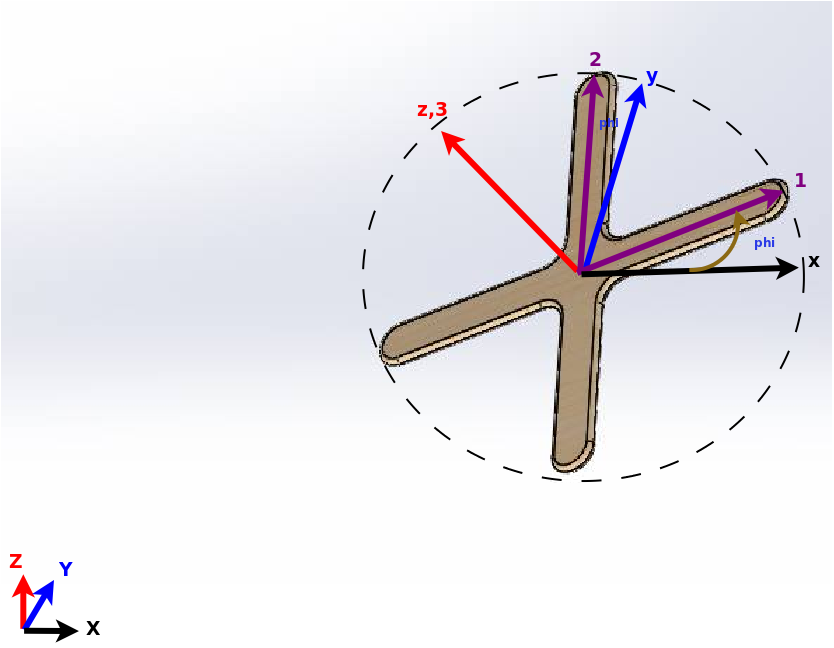
\includegraphics[scale=0.15]{imagenes/3-boomerang/sistemas_coordenados.png}
		\caption{Sistemas coordenados (X,Y,Z),(x,y,z),(1,2,3).}
		\label{fig12}
		\end{center}
		\end{figure}


	Para comenzar con el análisis, primero se derivarán las ecuaciones de movimiento del boomerang con respecto al sistema (x,y,z), desde que el sistema esta directamente relacionado con el estado de movimiento del boomerang con respecto al aire. El sistema (x,y,z) rota a una velocidad angular:


		\begin{equation}
		\vec{\Omega} = (\Omega_{x},\Omega_{y},\Omega_{z})
		\label{ec7}
		\end{equation} %% pag 80

	$\Omega_{z}$ esta determinada cinemáticamente por el hecho de que la componente ``y'' de la velocidad del centro de masa del boomerang es cero por definición. El movimiento del boomerang se puede separar en 2 partes:

		\begin{enumerate}
		\item{Movimiento del centro de masa.}
		\item{Movimiento del cuerpo con respecto a su centro de masa.}
		\end{enumerate}

	\subsubsection{Movimiento del centro de masa.}

	La velocidad del centro de masa del boomerang esta dada por:

		\begin{equation}
		\vec{V} = (V_{x},V_{y},V_{z})
		\label{ec8}
		\end{equation} %% pag 81


	donde las componentes están dadas en las direcciones x,y,z respectivamente. Por la deficición del sistema (x,y,z), tenemos:

		\begin{subequations}
		\begin{align}
    	V_{x} < 0 \\
		V_{y} = 0
		\end{align}
		\label{ec9}
		\end{subequations} %% pag 81

	Además dada la fuerza $\vec{F}$ como la fuerza resultante actuando sobre el boomerang, m la masa del boomerag, se tiene la fuerza expesada en relación del cambio del momento lineal:

		\begin{subequations}
		\begin{align}
		\vec{F} = \dot{\vec{P}} \\
		\vec{P} = m\vec{V}
		\end{align}
		\label{ec10}
		\end{subequations} %% pag 81

	Se llega a lo siguiente:

		\begin{equation}
		\vec{F} = {d\vec{p}\over dt} = \left({d\vec{p}\over dt} \right)^{\prime} + \vec{\Omega} \times \vec{p}
		\label{ec11}
		\end{equation} %% pag 81

	Utilizando (\ref{ec9}), tenemos:

		\begin{equation}
		\begin{bmatrix}
  		F_{x}\\
  		F_{y}\\
  		F_{z}
  		\end{bmatrix} =
  		m \dot{\vec{V}} + \vec{\Omega} \times m \vec{V} =
  		m \begin{bmatrix}
  		\begin{matrix}
  		\dot{V_{x}}\\
  		\dot{V_{y}}\\
  		\dot{V_{z}}\\
  		\end{matrix}
		+
		\begin{pmatrix}
        \Omega_{x}\\
        \Omega_{y}\\
        \Omega_{z}\\
		\end{pmatrix}
    	\times
		\begin{pmatrix}
        V_{x}\\
        V_{y}\\
        V_{z}\\
   		\end{pmatrix}
  		\end{bmatrix}
  		=
  		m \begin{bmatrix}
  		\begin{matrix}
  		\dot{V_{x}}\\
  		\dot{V_{y}}\\
  		\dot{V_{z}}\\
  		\end{matrix}
		+
		\begin{pmatrix}
        \Omega_{y}V_{z}-\Omega_{z}V_{y}\\
        \Omega_{x}V_{z}-\Omega_{z}V_{x}\\
        \Omega_{x}V_{y}-\Omega_{y}V_{x}\\
   		\end{pmatrix}
  		\end{bmatrix}
		\label{ec12}
		\end{equation} %% pag 81

	resultando:

		\begin{equation}
		\begin{bmatrix}
  		F_{x}\\
  		F_{y}\\
  		F_{z}
	  	\end{bmatrix} =
  		m \begin{bmatrix}
  		\begin{matrix}
  		\dot{V_{x}} + \Omega_{y}V_{z}\\
	    \Omega_{x}V_{z}-\Omega_{z}V_{x} \\
  		\dot{V_{z}}-\Omega_{y}V_{x}\\
   		\end{matrix}
  		\end{bmatrix}
		\label{ec13}
		\end{equation} %% pag 81

	La segunda ecuación de (\ref{ec13}) determina el valor de $\Omega_{z}$. Las solución exacta de las ecuaciones de (\ref{ec13}) son remplazadas por las ecuaciones  aproximadas o suavizadas:

		\begin{equation}
		\begin{bmatrix}
  		\bar{F_{x}}\\
  		\bar{F_{y}}\\
  		\bar{F_{z}}
  		\end{bmatrix} =
  		m \begin{bmatrix}
  		\begin{matrix}
  		\dot{\bar{V_{x}}} + \bar{\Omega_{y}}\bar{V_{z}}\\
    	\bar{\Omega_{x}}\bar{V_{z}}-\bar{\Omega_{z}}\bar{V_{x}} \\
  		\dot{\bar{V_{z}}}-\bar{\Omega_{y}}\bar{V_{x}}\\
   		\end{matrix}
  		\end{bmatrix}
		\label{ec14}
		\end{equation} %% pag 81

	En las ecuaciones (\ref{ec14}) las barras denotan las cantidades suavizadas. Las fuerzas $\bar{F_{x}}$, $\bar{F_{y}}$, $\bar{F_{z}}$ son fuerzas promediadas ó suavizadas. Las demás cantidades son resueltas por completo, por las ecuaciones de movimiento. La solución no será exacta desde que (\ref{ec14}) no son exactas. Pero proporcionan una aproxación razonable para el movimiento del centro de masa.

		\subsubsection{Movimiento con respecto al centro de masa.}

	Dada la velocidad angular del boomerang $\vec{\omega} = (\omega_{x},\omega_{y},\omega_{z})$ . Por definición del sistema x,y,z:

		\begin{subequations}
		\begin{align}
		\Omega_{x} = \omega_{x} \\
		\Omega_{y} = \omega_{y}
		\end{align}
		\label{ec15}
		\end{subequations} %% pag 82

	Dado $\bar{T}$ como el par resultante actuando en el boomerang y $\vec{L}$ el vector del momento angular del boomerang:

		\begin{equation}
		\vec{T} = \dot{\vec{L}}
		\label{ec16}
		\end{equation} %% pag 82

	y

	    \begin{equation}
		\vec{T} = {d\vec{L}\over dt} = \left({d\vec{L}\over dt} \right)^{\prime} + \vec{\Omega} \times \vec{L}
		\label{ec17}
		\end{equation} %% pag 82

	Resultando:

		\begin{equation}
		\begin{bmatrix}
  		T_{x}\\
  		T_{y}\\
  		T_{z}
  		\end{bmatrix} =
  		\begin{bmatrix}
  		\begin{matrix}
  		\dot{L_{x}}\\
  		\dot{L_{y}}\\
  		\dot{L_{z}}\\
  		\end{matrix}
		+
        \begin{pmatrix}
        \Omega_{x}\\
        \Omega_{y}\\
        \Omega_{z}
		\end{pmatrix}
    	\times
        \begin{pmatrix}
        L_{x}\\
        L_{y}\\
        L_{z}
		\end{pmatrix}
  		\end{bmatrix}
  		=
  		m \begin{bmatrix}
  		\begin{matrix}
  		\dot{L_{x}}\\
  		\dot{L_{y}}\\
  		\dot{L_{z}}\\
  		\end{matrix}
		+
	    \begin{pmatrix}
        \Omega_{y}L_{z}-\Omega_{z}L_{y}\\
        \Omega_{x}L_{z}-\Omega_{z}L_{x}\\
        \Omega_{x}L_{y}-\Omega_{y}L_{x}
		\end{pmatrix}
  		\end{bmatrix}
		\label{ec18}
		\end{equation} %% pag 81

	Para obtener $L_{x}, L_{y}$ y $L_{z}$ es necesario considerar el sistema (1,2,3). Tomando en cuenta que el eje 3 coincide con el eje z, se observa un ángulo $\phi$ en el plano (x,y) con el plano (1,2), entonces:

    	\begin{subequations}
    	\begin{align}
    	\dot{\phi} = \omega_{3}-\Omega_{z}\\
    	\omega_{3} = \omega_{z}
		\end{align}
		\label{ec19}
		\end{subequations} %% pag 82

	Los componentes del momento angular con respecto al sistema (1,2,3) están relacionados con el momento de inercia prinicipal de la siguiente manera:

		\begin{subequations}
    	\begin{align}
    	L_{1} = I_{1}\Omega_{1}\\
    	L_{2} = I_{2}\Omega_{2}\\
    	L_{3} = I_{3}\Omega_{3}
		\end{align}
		\label{ec20}
		\end{subequations} %% pag 82

	La matriz de transformación del sistema (1,2,3) al sistema (x,y,z) y viceversa esta dado por:

		\begin{equation}
    	R = \bordermatrix{~ & 1 & 2 & 3 \cr
        x & cos(\phi) & -sen(\phi) & 0 \cr
        y & sen(\phi) &  cos(\phi) & 0 \cr
        z & 0       &  0       & 1 \cr }
    	\label{ec21}
    	\end{equation}

    Por lo que obtenemos:

		\begin{equation}
		\begin{bmatrix}
  		{L_{x}}\\
  		{L_{y}}\\
  		{L_{z}}
  		\end{bmatrix} =
 		\begin{pmatrix}
        & cos(\phi) & -sen(\phi) & 0 \\
        & sen(\phi) &  cos(\phi) & 0 \\
        & 0       &  0       & 1
		\end{pmatrix}
    	\begin{bmatrix}
  		L_{1}\\
  		L_{2}\\
  		L_{3}
  		\end{bmatrix}
  		=
    	\begin{bmatrix}
  		cos(\phi) L_{1} - sen(\phi) L_{2} \\
  		sen(\phi) L_{1} + cos(\phi) L_{2} \\
  		L_{3}
  		\end{bmatrix}
  		=
    	\begin{bmatrix}
  		cos(\phi) I_{1} \omega_{1} - sen(\phi) I_{2} \omega_{2} \\
  		sen(\phi) I_{1} \omega_{1} + cos(\phi) I_{2} \omega_{2} \\
  		I_{3} \omega_{3}
  		\end{bmatrix}
		\label{ec22}
		\end{equation} %% pag 81

		\begin{equation}
		\begin{bmatrix}
  		{\omega_{1}}\\
  		{\omega_{2}}\\
  		{\omega_{3}}
  		\end{bmatrix} =
 		\begin{pmatrix}
        & cos(\phi) & sen(\phi) & 0 \\
        & -sen(\phi) &  cos(\phi) & 0 \\
        & 0       &  0       & 1
		\end{pmatrix}
    	\begin{bmatrix}
  		w_{x}\\
  		w_{y}\\
  		w_{z}
  		\end{bmatrix}
  		=
    	\begin{bmatrix}
  		cos(\phi) w_{x} + sen(\phi) w_{y}\\
   		-sen(\phi) w_{x} + cos(\phi) w_{y}\\
  		\omega_{z}
  		\end{bmatrix}
		\label{ec23}
		\end{equation} %% pag 81

	Sustiyendo (\ref{ec23}) en (\ref{ec22}):

    	\begin{equation}
		\begin{bmatrix}
  		{L_{x}}\\
  		{L_{y}}\\
  		{L_{z}}
  		\end{bmatrix} =
 		\begin{pmatrix}
        \frac{1}{2}(I_{1}+I_{2})\omega_{x} + \frac{1}{2}(I_{1}-I_{2})(\omega_{x}cos(2\phi)+\omega_{y}sen(2\phi)) \\
        \frac{1}{2}(I_{1}+I_{2})\omega_{y} + \frac{1}{2}(I_{1}-I_{2})(\omega_{x}sen(2\phi)+\omega_{y}cos(2\phi)) \\
        \omega_{z}
		\end{pmatrix}
		\label{ec24}
		\end{equation} %% pag 81

	Utilizando (\ref{ec19}) obtenemos por diferencición de (\ref{ec22}):

		\begin{equation}
		\begin{bmatrix}
	  	\dot{L_{x}}\\
  		\dot{L_{y}}\\
  		\dot{L_{z}}
  		\end{bmatrix} =
 		\begin{pmatrix}
 		I_{1}\dot{\omega_{1}}cos(\phi)-I_{2}\dot{\omega_{2}}sen(\phi)+(\omega_{3}-\Omega_{z})(-I_{1}\omega_{1}sin(\phi)+I_{2}\omega_{2}cos(\phi))\\
   		I_{1}\dot{\omega_{1}}sin(\phi)+I_{2}\dot{\omega_{2}}cos(\phi)+(\omega_{3}-\Omega_{z})(I_{1}\omega_{1}cos(\phi)-I_{2}\omega_{2}sin(\phi))\\
        I_{3}\dot{\omega_{3}}
		\end{pmatrix}
		\label{ec25}
		\end{equation} %% pag 81

	y por diferenciación de (\ref{ec23}) se obtiene:

		\begin{equation}
		\begin{bmatrix}
  		\dot{\omega_{1}}\\
  		\dot{\omega_{2}}\\
  		\dot{\omega_{3}}
  		\end{bmatrix} 	=
    	\begin{bmatrix}
  		\dot{\omega_{x}}cos(\phi) + \dot{\omega_{y}}sen(\phi) + (\omega_{z}-\Omega_{z})(-w_{x} sen(\phi) + w_{y}cos(\phi)) \\
  		-\dot{\omega_{x}}sen(\phi) + \dot{\omega_{y}}cos(\phi) + (\omega_{z}-\Omega_{z})(-w_{x} cos(\phi) - w_{y}sen(\phi)) \\
  		\dot{\omega_{z}}
  		\end{bmatrix}
		\label{ec26}
		\end{equation} %% pag 81

	Sustituyendo (\ref{ec23}) y (\ref{ec26}) en (\ref{ec25}):

		\begin{equation}
		\begin{bmatrix}
	  	\dot{L_{x}}\\
  		\dot{L_{y}}\\
  		\dot{L_{z}}
  		\end{bmatrix} =
 		\begin{pmatrix}
 		\frac{1}{2}(I_{1}+I_{2})\dot{\omega{x}} + \frac{1}{2}(I_{1}-I_{2})(-\dot{\omega_{x}}cos(2\phi)+\dot{\omega_{y}}sen(2\phi))+ (I_{1}-I_{2})(\omega_{z}-\Omega_{z})(-{\omega_{x}}sen(2\phi)+{\omega_{y}}cos(2\phi))\\
 		\frac{1}{2}(I_{1}+I_{2})\dot{\omega{y}} + \frac{1}{2}(I_{1}-I_{2})( \dot{\omega_{x}}sen(2\phi)+\dot{\omega_{y}}cos(2\phi))+ (I_{1}-I_{2})(\omega_{z}-\Omega_{z})({\omega_{x}}cos(2\phi)+{\omega_{y}}sen(2\phi))\\
 		I_{3}\dot{\omega_{3}}
		\end{pmatrix}
		\label{ec27}
		\end{equation} %% pag 81

	Utlizando (\ref{ec22})	y (\ref{ec27}) en (\ref{ec18}) y recurriendo a (\ref{ec15}):

		\begin{equation}
		\begin{bmatrix}
	  	{T_{x}}\\
  		{T_{y}}\\
  		{T_{z}}
  		\end{bmatrix} =
  		\begin{pmatrix}
 		\begin{smallmatrix}
        \frac{1}{2}(I_{1}+I_{2})\dot{\omega_{x}} - \frac{1}{2}(I_{1}+I_{2})\omega_{y}\Omega_{z} + I_{3}\omega_{z}\omega_{y} + \frac{1}{2}(I_{1}-I_{2})(-\dot{\omega_{x}}cos(2\phi)+\dot{\omega_{y}}sen(2\phi)) + \frac{1}{2}(I_{1}-I_{2})(2\omega_{z}-\Omega_{z})(-\omega_{x}sen{2\phi}+\omega_{y}cos{2\phi})\\
        \frac{1}{2}(I_{1}+I_{2})\dot{\omega_{y}} + \frac{1}{2}(I_{1}+I_{2})\omega_{x}\Omega_{z} - I_{3}\omega_{z}\omega_{y} + \frac{1}{2}(I_{1}-I_{2})(-\dot{\omega_{x}}sen(2\phi)+\dot{\omega_{y}}cos(2\phi)) + \frac{1}{2}(I_{1}-I_{2})(2\omega_{z}-\Omega_{z})(\omega_{x}cos{2\phi}+\omega_{y}sen{2\phi})\\
        I_{3}\dot{\omega_{z}}+(I_{1}-I_{2})[(\omega_{x}^{2}+\omega_{y}^{2})sen(2\phi)-\omega_{x}\omega_{y}cos(2\phi)]
		\end{smallmatrix}
  		\end{pmatrix}
		\label{ec28}
		\end{equation} %% pag 81

	Para nuestro boomerang se cumple $I_{1}=I_{2}=I_{12}$, la ecuación (\ref{ec28}) se reduce a:

		\begin{equation}
		\begin{bmatrix}
	  	{T_{x}}\\
  		{T_{y}}\\
  		{T_{z}}
  		\end{bmatrix} =
  		\begin{pmatrix}
        I_{12}\dot{\omega_{x}} + (I_{3}\omega_{z}-I_{12}\Omega_{z})\omega_{y}\\
        I_{12}\dot{\omega_{y}} - (I_{3}\omega_{z}-I_{12}\Omega_{z})\omega_{x}\\
        I_{3}\dot{\omega_{z}}
  		\end{pmatrix}
		\label{ec29}
		\end{equation} %% pag 81

	las cuales son las ecuaciones para una vista simétrica cn respecto al sistema (x,y,z). Hasta este punto todas las ecuaciones son exactas. Las ecuaciones (\ref{ec28}) se suavizan de la siguiente manera:

		\begin{equation}
		\begin{bmatrix}
	  	\bar{T_{x}}\\
  		\bar{T_{y}}\\
  		\bar{T_{z}}
  		\end{bmatrix} =
  		\begin{pmatrix}
        I_{12}\bar{\dot{\omega_{x}}} + (I_{3}\bar{\omega_{z}}-I_{12}\bar{\Omega_{z}})\bar{\omega_{y}}\\
        I_{12}\bar{\dot{\omega_{y}}} - (I_{3}\bar{\omega_{z}}-I_{12}\bar{\Omega_{z}})\bar{\omega_{x}}\\
        I_{3}\bar{\dot{\omega_{z}}}
  		\end{pmatrix}
		\label{ec30}
		\end{equation} %% pag 81

	Una segunda simplificación puede ser echa, para los boomerang que giran rápidamente, generalmente se tiene:

		\begin{subequations}
    	\begin{align}
    	\| \bar{\omega_{x}} \| , \| \bar{\omega_{x}} \|, \| \bar{\Omega_{x}} \| << \| \bar{\omega_{z}} \| \\
    	\| \bar{\dot{\omega_{x}}} \| << \| \bar{\omega_{y}}\bar{\omega_{z}} \| , \| \bar{\dot{\omega_{y}}} \| << \| \bar{\omega_{x}}\bar{\omega_{z}} \|
    	\end{align}
		\label{ec31}
		\end{subequations} %% pag 82

	De esta manera se obtiene una aproximación de (\ref{ec30}):

		\begin{equation}
		\begin{bmatrix}
	  	\bar{T_{x}}\\
  		\bar{T_{y}}\\
  		\bar{T_{z}}
  		\end{bmatrix} =
  		\begin{pmatrix}
         I_{3}\bar{\omega_{z}}\bar{\omega_{y}}\\
        -I_{3}\bar{\omega_{z}}\bar{\omega_{x}}\\
        I_{3}\bar{\dot{\omega_{z}}}
  		\end{pmatrix}
		\label{ec32}
		\end{equation}

	Las ecuaciones (\ref{ec14}) y (\ref{ec32}) serán utilizadas para el cálculo de la trayectoria del vuelo del boomerang.

	\subsubsection{Ecuaciones de movimiento II}

	Las ecuaciones de movimiento de un boomerang respecto al sistema coordenado (x, y, z) son dadas por las ecuaciones (\ref{ec14}) y (\ref{ec32}) , pero ahora usaremos las variables suavizadas o promediadas exclusivamente omitiendo las barras superiores.

	En esta sección obtendremos las ecuaciones de movimiento respecto al sistema inercial fijo (X, Y, Z), en el cual el eje Z apunta verticalmente hacia arriba y el plano  (Y, Z) es horizontal. La relación entre este sistema de referencia y el sistema (x, y, z) es dada por los angulos de euler $\phi$, $\eta$ y $\vartheta$ como se muestra en la Fig. (\ref{fig13}), donde, por definición $0\le \vartheta \le \pi$.

		\begin{figure}[ht]
		\begin{center}
		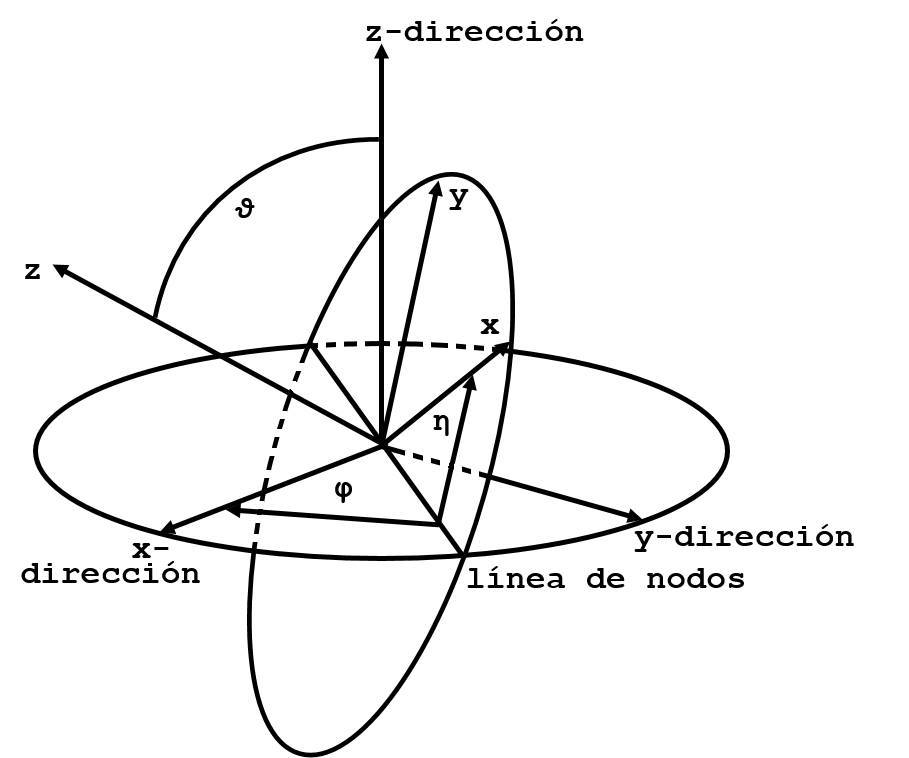
\includegraphics[scale=0.3]{imagenes/3-boomerang/euler_angles.png}
		\caption{Angulos de euler definiendo la relacion entre los sistemas coordenados (x, y, z) y (X, Y, Z).}
		\label{fig13}
		\end{center}
		\end{figure}

	La transformación que lleva un vector en (x, y, z) a su representación en el sistema de referencia (X, Y, Z) es la siguiente:

		\begin{equation}
  		\bordermatrix{ ~ & x & y & z \cr
		X & cos { \eta } cos { \varphi -cos { \vartheta } sen { \varphi } sen { \eta } } & -sen { \eta } cos { \varphi } -cos { \vartheta } sen { \varphi } cos { \eta } & sen { \vartheta } sen { \varphi } \cr
		Y & cos { \eta } sen { \varphi } +cos { \vartheta } cos { \varphi } sen { \eta } & -sen { \eta } sen { \varphi } +cos { \vartheta } cos { \varphi } cos { \eta } & -sen { \vartheta } cos { \varphi } \cr
		Z & sen { \vartheta } sen { \eta } & sen { \vartheta } cos { \eta } & cos { \vartheta }  \cr
		}
		\label{ec33}
		\end{equation}

	Para la velocidad angular $\vec { \Omega  }$  del sistema de referencia (x, y, z) ahora tenemos:

		\begin{equation}
		\begin{bmatrix}
		\Omega_{x} \\
		\Omega_{y} \\
		\Omega_{z}
		\end{bmatrix} =
		\begin{pmatrix}
	    \dot{\vartheta}cos{\eta + \dot{\varphi}sen{\vartheta}sen{\eta}} \\
		-\dot{\vartheta}sen{\eta}+\dot{\varphi}sen{\vartheta}cos{\eta}\\
		\dot{\eta}+\dot{\varphi}cos{\vartheta}
  		\end{pmatrix}
		\label{ec34}
		\end{equation}

		lo que lleva a:

		\begin{equation}
		\begin{bmatrix}
		\dot{\vartheta}\\
		\dot{\varphi}\\
     	\dot{\eta}
		\end{bmatrix} =
		\begin{pmatrix}
		{\Omega}_{x}cos{\eta}-{\Omega}_{y}\sin{\eta}\\
		\frac{1}{\sin{\vartheta}}({\Omega}_{x}\sin{\eta}+{\Omega}_{y}cos{\eta})\\
		{\Omega}_{z}-\frac{cos{\vartheta}}{\sin{\vartheta}}({\Omega}_{x}\sin{\eta}+{\Omega}_{y}cos{\eta})
		\end{pmatrix}
		\label{ec34}
		\end{equation}

	De (\ref{ec15}) y (\ref{ec32})  obtenemos:

		\begin{equation}
		\begin{matrix}
		\Omega_{x}={\omega}_{x}=-\frac{{T}{y}}{{I}_{3}{\omega}_{z}}\\
		\Omega_{y}={\omega}_{y}=\frac{{T}_{x}}{{I}_{3}{\omega}_{z}}\\
		\dot{\omega}_{z}=\frac{{T}_{z}}{{I}_{3}}
		\end{matrix}
		\label{ec35}
		\end{equation}

	y de (\ref{ec14}) :

		\begin{equation}
		\begin{matrix}
		\Omega_{z}=\frac{{F}_{y}}{m{V}_{x}}+\frac{{V}_{z}{\omega}_{x}}{{V}_{x}}\\
		\dot{V}_{x}=\frac{{F}_{x}}{m}-{V}_{x}{\omega}_{y}\\
		\dot{V}_{z}=\frac{{F}_{z}}{m}+{V}_{x}{\omega}_{y}
		\end{matrix}
		\label{ec36}
		\end{equation}


	Introducimos las variables V y $\Psi$  definidos por:

		\begin{equation}
		\begin{matrix}
		V_{x}=-Vcos{\Psi}\\
		V_{z}=-V\sin{\Psi}\\
		V>0,\quad\left|\Psi\right|<\cfrac{1}{2}\pi
		\end{matrix}
		\label{ec37}
		\end{equation}

	Recuerdese que $Vx<0$ y Vy = 0  son los componentes sobre los ejes x $\&$ y respectivamente de la velocidad lineal del boomerang (V), Psi es el ángulo entre la parte negativa del eje x y la dirección de la velocidad del boomerang. Llamamos a $\Psi$ el ángulo de incidencia. Entonces (\ref{ec36}) puede ser escrito como:

		\begin{equation}
		\begin{matrix}
		\Omega_{z}=-\frac{{F}_{y}}{mVcos{\Psi}}+{\omega}_{x}\tan{\Psi}\\
		\dot{V}=\frac{1}{m}(-{F}_{x}cos{\Psi}-{F}_{z}\sin{\Psi})\\
		\dot{\Psi}=\frac{1}{mV}({F}_{x}\sin{\Psi-{F}_{z}cos{\Psi}})+{\omega}_{y}
		\end{matrix}
		\label{ec38}
		\end{equation}

	Las ecuaciones (\ref{ec34}), (\ref{ec35}) y (\ref{ec38}) determinan el movimiento del boomerang y pueden combinarse formando:

		\begin{equation}
		\begin{matrix}
		\dot{\omega}_{z}=\frac{T_{y}}{{I}_{3}}\\
		\dot{V}=\frac{1}{m}(-{F}_{x}cos{\Psi}-{F}_{z}\sin{\Psi})\\
		\dot{\Psi}=\frac{1}{m }({F}_{x}\sin{\Psi-{F}_{z}cos{\Psi}})+\frac{{T}_{x}}{{I}_{3}{\omega}_{z}}
		\end{matrix}
		\label{ec39}
		\end{equation}

		\begin{equation}
		\begin{matrix}
		 {\dot{\vartheta}}_{z}=\frac{1}{{I}_{3}{\omega}_{z}}(-{T}_{y}cos{\eta}-{T}_{x}\sin{\eta})\\
		 \dot{\varphi}=\frac{1}{{I}_{3}{\omega}_{z}}\frac{1}{\sin{\vartheta}}(-{T}_{y}\sin {\eta}+{T}_{x}cos{\eta})\\
		 \dot{\eta}=-\frac{{F}_{y}}{mVcos{\Psi}}-\tan{\Psi}\frac{T_{y}}{{I}_{3}{\omega}_{z}}-\dot{\varphi} cos{\vartheta}
		\end{matrix}
		\label{ec40}
		\end{equation}

	Para la posición del centro de masa del boomerang en el sistema de referencia (X, Y, Z) tenemos simplemente:

		\begin{equation}
		\begin{matrix}
		\dot{X} = V[{-cos{\Psi}(cos{\eta}cos{\varphi}-\sin{\eta}\sin{\varphi}cos{\vartheta})-\sin{\Psi}\sin{\varphi}\sin{\vartheta}]}\quad\\
	    \dot{Y}=V[{-cos{\Psi}\left(cos{\eta}\sin{\varphi}+\sin{\eta}cos{\varphi}cos{\vartheta}\right)+\sin{\Psi}cos{\varphi}\sin{\vartheta}]}\\
	    \dot{Z}=V[{-cos{\Psi\sin{\eta}\sin{\vartheta}-\sin{\Psi}cos{\vartheta}}]}
		\end{matrix}
		\label{ec41}
		\end{equation}

	Las ecuaciones (\ref{ec39}), (\ref{ec40}) y (\ref{ec41}) deben ser integradas numericamente. Las fuerzas y pares $F_{x}$, $F_{y}$, $F_{z}$, $T_{x}$, $T_{y}$, $T_{z}$ deben ser dados como funciones conocidas del estado de movimiento del sistema. Si las condiciones iniciales son proveidas, estas nueve ecuaciones diferenciales de primer orden pueden ser resueltas para las nueve incognitas $\omega_{z}$, V, $\Psi$, $\vartheta$, $\varphi$, $\eta$, X, Y, Z como funciones del tiempo, t.

	Las ecuaciones (\ref{ec39}) y (\ref{ec40})  contienen singularidades si las variables del denominador se vuelven triviales, lo cual ocurre en los cuatro casos siguientes:

		\begin{equation}
		\begin{matrix}
	    \sin{\vartheta\rightarrow}0\\
		cos{\Psi\rightarrow}0\\
		{V\rightarrow}0\\
		{{\omega}_{z}\rightarrow}0
		\end{matrix}
		\label{ec42}
		\end{equation}

	% Consideremos los casos de uno por uno.

	\subsection{Fuerzas actuantes sobre el boomerang}

	Consideremos las siguientes suposiciones concernientes al boomerang, el medio en el cual se mueve y la gravedad:

	\begin{enumerate}
	\item El boomerang es un cuerpo rígido. Su tamaño se caracteriza por su radio a, el cual es el radio que describe el boomerang al girar sobre su centro de masa. La masa del boomerang es m, y sus momentos principales de inercia, de menor a mayor magnitud, son I$_{1}$, I$_{2}$, I$_{3}$; y su densidad promedio es $\rho$.
	\item El medio es homogeneo, isotrópico, constante en el tiempo, de extensión finita. Su densidad es $\mu$, su viscosidad cinemática es $\nu$. No se consideran efectos aerodinámicos o aerodinámicos debidos a la presencia de objetos como la tierra o arboles.
	\item La aceleración de la gravedad, $\vec{g}$, se considera constante y dirigida hacia abajo, en la dirección negativa de Z
	\end{enumerate}

	Las fuerzas actuantes sobre el boomerang son de dos tipos: fuerzas debidas a la gravedad y fuerzas debidas a la interacción con el aire, denotadas por un subíndice g y a respectivamente. Entonces:

		\begin{subequations}
    	\begin{align}
	    \vec{F}={\vec{F}}_{g}+{\vec{F}}_{a}\\
    	\vec{T}={\vec{T}}_{a}
		\end{align}
		\label{ec43}
		\end{subequations}

	Los componentes de $({\vec{F}}_{g})$ en el sistema (X, Y, Z) son:

		\begin{equation}
    	{\vec{F}}_{g}=-mg(\sin{\vartheta}\sin{\eta},\sin{\vartheta}cos{\eta},cos{\vartheta})
		\label{ec44}
		\end{equation}

	Las fuerzas hidrostáticas pueden ser tomadas en cuenta reemplazando g por:

		\begin{equation}
		{g}^{\prime}=g(1-\cfrac{{\mu}}{\rho})
		\label{ec45}
		\end{equation}

	No es tan simple obtener expresiones para las fuerzas aerodinámicas, las cuales pueden depender de:

		\begin{enumerate}[a)]
		\item Las propiedades del aire: e. g. Densidad, viscosidad, turbulencia.
		\item La forma del boomerang.
		\item el estao de movimiento del boomerang: e.g.  $\Psi$ , $\vec{\omega}$ , V.
		\item historial previo
		\end{enumerate}

	De acuerdo con los metodos de analisis dimensional, los componentes en (x, y, z) de ${\vec{F}}_{a}$ pueden ser escritos en la forma:

		\begin{equation}
		\vec{F}_{a}={\mu}_{a}{a}^{2}{V}^{2}\vec{f}(\Psi,\cfrac{V}{{\omega}_{z}a},\cfrac{{\omega}_{x}}{{\omega}_{z}},\cfrac{{\omega}_{y}}{{\omega}_{z}},\phi,Re,Historial,Forma)
		\label{ec46}
		\end{equation}

	donde todos los argumentos de  $\vec{f}$ son adimensionales. $Re=\frac{aV}{\nu}$ es un número de Reynolds. El historial representa la influencia de condiciones previas en el vuelo del boomerang. La forma denota un conjunto de parametros adimensionales que definen la forma del boomerang (no el tamaño). El factor ${V}^{2}$ en (\ref{ec46}) puede ser reemplazado por $({\omega}_{z}a)^{2}$, si se desea. ${\vec{T}}_{a}$ puede ser escrito de forma similar con un factor adicional a. Es el historial el que acarrea las mayores dificultades, ya que puede depender del completo movimiento del boomerang desde su inicio, t $=$ 0, hasta su instante presente, t $=$ tp.

	Bajo la base de muchas suposiciones, la función desconocida $\vec{f}$ en (\ref{ec46}) puede ser simplificada. Ya que trabajaremos con fuerzas promediadas (suavizadas), una enorme cantidad de simplificaciones pueden ser tomadas sobre un periodo de $\phi$ , y reemplazar el historial por uno ficticio en el cual las cantidades

		\begin{equation}
		\Psi,\cfrac{V}{{\omega}_{z}a},\cfrac{{\omega}_{x}}{{\omega}_{z}},\cfrac{{\omega}_{y}}{{\omega}_{z}},Re
		\label{ec47}
		\end{equation}

	son constantes para todo $t\le{t}_{p}$ . Esto es una aproximación cuasi-estacionaria. La situación en
  	$t={t}_{p}$, para el propósito de calcular fuerzas aerodinámicas, se supone constante para $-\infty <t\le{t}_{p}$. La parte previa de la trayectoria de vuelo del boomerang es reemplazada por una línea recta. Este historial extremadamente simplificado depende solo de la situación presente $(t={t}_{p})$, y deja de ser un conjunto de variables independientes en (\ref{ec46}), por lo que obtenemos:

		\begin{equation}
		{\vec{F}}_{a}={\mu}{a}^{2}{V}^{2}\vec{f}(\Psi,U,\cfrac{{\omega}_{x}}{{\omega}_{z}},\cfrac{{\omega}_{y}}{{\omega}_{z}},Re,Forma)
		\label{ec48}
		\end{equation}

	donde U es la raza de avance, definida como:

		\begin{equation}
		U=\frac{V}{{\omega}_{z}a}
		\label{ec49}
		\end{equation}

	La dependencia de Re no es del todo despreciable, \cite{Hess1975} mostró en experimentos en túnel de viento que tiene cierta influencia. Sin embargo las fuerzas computadas por su modelo del ala son independientes de Re. Para el propósito del cálculo de la trayectoria de vuelo del boomerang asumiremos que la influencia de este número es despreciable y por lo tanto, tenemos:

		\begin{equation}
		{\vec{F}}_{a}={\mu}{a}^{2}{V}^{2}\vec{f}(\Psi,U,\cfrac{{\omega}_{x}}{{\omega}_{z}},\cfrac{{\omega}_{y}}{{\omega}_{z}},Forma)
		\label{ec50}
		\end{equation}

	Si $\frac{{\omega}_{x}}{{\omega}_{z}}$ y $\frac{{\omega}_{y}}{{\omega}_{z}}$ son muy pequeñas, no tendrán una influencia significativa en ${\vec{F}}_{a}$ y ${\vec{T}}_{a}$ , y estos parámetros pueden ser omitidos de (\ref{ec50}(. Esta suposición no es necesaria, sin embargo, como se muestra a continuación:

		\begin{subequations}
    	\begin{align}
    	{\vec{F}}_{a}={\mu}{a}^{2}{V}^{2}{\vec{F}}_{0}(\Psi,I/U)\\
    	{\vec{T}}_{a}={\mu}{a}^{3}{V}^{2}{\vec{T}}_{0}(\Psi,I/U)
		\end{align}
		\label{ec51}
		\end{subequations}

	o, alternativamente, como:

		\begin{subequations}
    	\begin{align}
		{\vec{F}}_{a}={\mu}{a}^{4}{\omega}_{z}^{2}{\vec{F}}_{1}(\Psi,U)\\
		{\vec{T}}_{a}={\mu}{a}^{5}{\omega}_{z}^{2}{\vec{T}}_{1}(\Psi,U)
		\end{align}
		\label{ec52}
		\end{subequations}

	donde ${\vec{F}}_{0}$ y ${\vec{T}}_{0}$ o ${\vec{F}}_{1}$ y ${\vec{T}}_{1}$ también dependen de la forma del boomerang. Durante vuelos reales del boomerang, la velocidad V varía fuertemente, mientras que las variaciones relativas en la velocidad de rotación ${\omega}_{z}$ son menores al 20$\%$. Por lo tanto, parece conveniente utilizar (\ref{ec52}) en lugar de (\ref{ec51}), esto es, durante el vuelo del boomerang, las variables adimensionales ${\vec{F}}_{1}$ y ${\vec{T}}_{1}$ se comportan practicamente como ${\vec{F}}_{a}$ y ${\vec{T}}_{a}$.

	Finalmente, reconsideremos la suposición del desvanecimiento de ${ \omega }_{ x } y { \omega }_{ y }$. La restricción impuesta por esto puede ser removida. En lugar de (5.10) ahora tenemos:


	\subsection{La influencia del viento}

	La influencia del viento en el movimiento del boomerang debe de ser tomada en cuenta, esto puede incluirse fácilmente en las ecuaciones  (\ref{ec39}) y (\ref{ec40}). Se supone que el viento predominante puede ser descrito por el campo vectorial $\vec{W}(X,Y,Z,t)$  con los componentes $W_{X}$,$W_{Y}$ y $W_{Z}$ dados. Los componentes de esta velocidad con respecto al sistema (x,y,z) se obtiene por la matriz de transformación (\ref{ec33}). Por lo que la velocidad del boomerang con respecto al aire resulta:

		\begin{equation}
		\vec{V} - \vec{W} = ({Vx}-{Wx}, {-Wy}, {Vz}-{Wz}) = (-{V}cos{\Psi}-{Wx}, {-Wy}, -{V}sen{\Psi}-{Wz})
		\label{ec53}
		\end{equation}

	Desde que se trabaja con las ecuaciones suavizadas es necesario asumir que $\vec{V}-\vec{W}$ varía relativamente poco durante un periodo de giro del boomerang. Por lo tanto las flutuaciones repentinas en la velocidad del viento se descartan.

		\begin{figure}[ht]
		\begin{center}
		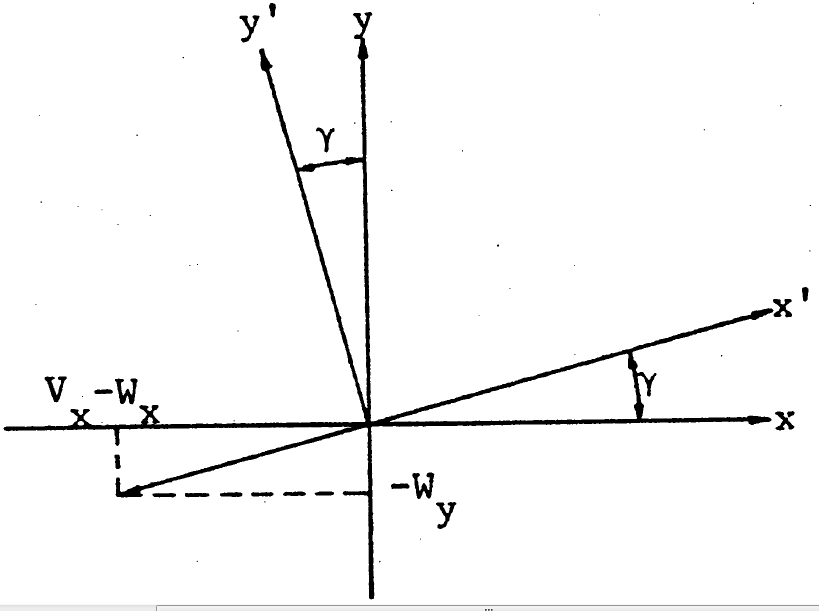
\includegraphics[scale=0.4]{imagenes/3-boomerang/vel_vient.png}
		\caption{Sistema coordenado (x,y,z) y (x$^\prime$,y$^\prime$,z$^\prime$).}
		\label{fig13}
		\end{center}
		\end{figure}

	Se introduce un nuevo sistema coordenado $(x^{\prime},y^{\prime},z^{\prime})$, de tal manera que la velocidad relativa en la dirección de $y^{\prime}$ del boomerang con respecto al bommerang desaparece. El ángulo $\gamma$ entre el eje $x$ y el eje $x^{\prime}$ esta dado por:

		\begin{equation}
		\gamma = arctan(\frac{W_{y}}{Vcos{\Psi}+W_{x}})
		\label{ec54}
		\end{equation}

	La trasformación del sistema coordenado $(x,y,z)$ al sistema coordenado $(x^{\prime},y^{\prime},z^{\prime})$ y viceversa esta determinada por:

		\begin{equation}
    	R = \bordermatrix{~ & x & y & z \cr
        x^{\prime} & cos(\gamma) & sen(\gamma) & 0 \cr
        y^{\prime} & -sen(\gamma) &  cos(\gamma) & 0 \cr
        z^{\prime} & 0       &  0       & 1 \cr }
    	\label{ec55}
    	\end{equation}

    Las componentes de la velocidad relativa del boomerang respecto al aire pueden ser reescritas por:

    	\begin{equation}
		\vec{V} - \vec{W} = (-\sqrt{(Vcos{\Psi}+W_{x})^{2}+W_{x})^{2}},0,-Vsen{\Psi}-W_{x})
		\label{ec56}
		\end{equation}

	donde las componentes estan dadas en el sistema coordenado $(x_{\prime},y_{\prime},z_{\prime})$. Agragando estos efectos a las ecuaciones de movimiento (\ref{ec39}) y (\ref{ec40}), $V$, $U$ y $\Psi$ deben ser reeplanzados por los valores relativos al movimiento del aire:

		\begin{subequations}
    	\begin{align}
		{V^{\prime}} = \sqrt{(Vcos{\Psi}+W_{x})^{2} + W_{y})^{2} + (Vsen{\Psi}+W_{z})^{2}}\\
	    = \sqrt{(V^{2} + W^{2} + 2V(W_{z}sen{\Psi} + W_{x}cos{\Psi})}
		\end{align}
		\label{ec57}
		\end{subequations}

    	\begin{equation}
		U^{\prime} = \frac{\vec{V^{\prime}}}{\omega_{z}a}
		\label{ec58}
		\end{equation}

		\begin{equation}
		{\Psi} = \arctan(\frac{W_{y}+Vsen{\Psi}}{\sqrt{(Vcos{\Psi}+W_{x})^{2} + W_{y})^{2}}})
		\label{ec59}
		\end{equation}


    \section{Simulador}

	En este capítulo se presenta un simulador basado en las ecuaciones de movimiento del boomerang obtenidas en el capítulo anterior, las cuales se muestran a continuación:

		\begin{equation}
		\begin{matrix}
		\dot{\omega}_{z}=\frac{T_{y}}{{I}_{3}}\\
		\dot{V}=\frac{1}{m}(-{F}_{x}\cos{\Psi}-{F}_{z}\sin{\Psi})\\
		\dot{\Psi}=\frac{1}{m }({F}_{x}\sin{\Psi-{F}_{z}\cos{\Psi}})+\frac{{T}_{x}}{{I}_{3}{\omega}_{z}} \\
		\end{matrix}\\
		\label{ec61}
		\end{equation}

		\begin{equation}
		\begin{matrix}
		 {\dot{\vartheta}}=\frac{1}{{I}_{3}{\omega}_{z}}(-{T}_{y}\cos{\eta}-{T}_{x}\sin{\eta})\\
		 \dot{\varphi}=\frac{1}{{I}_{3}{\omega}_{z}}\frac{1}{\sin{\vartheta}}(-{T}_{y}\sin {\eta}+{T}_{x}\cos{\eta})\\
		 \dot{\eta}=-\frac{{F}_{y}}{mV\cos{\Psi}}-\tan{\Psi}\frac{T_{y}}{{I}_{3}{\omega}_{z}}-\dot{\varphi} \cos{\vartheta} \\
		\end{matrix}
		\label{ec62}
		\end{equation}

		\begin{equation}
		\begin{matrix}
		\dot{X} = V[{-\cos{\Psi}(\cos{\eta}\cos{\varphi}-\sin{\eta}\sin{\varphi}\cos{\vartheta})-\sin{\Psi}\sin{\varphi}\sin{\vartheta}]}\quad\\
	    \dot{Y}=V[{-\cos{\Psi}\left(\cos{\eta}\sin{\varphi}+\sin{\eta}\cos{\varphi}\cos{\vartheta}\right)+\sin{\Psi}\cos{\varphi}\sin{\vartheta}]}\\
	    \dot{Z}=V[{-\cos{\Psi\sin{\eta}\sin{\vartheta}-\sin{\Psi}\cos{\vartheta}}]}
		\end{matrix}
		\label{ec63}
		\end{equation}

	Para las fuerzas y pares aerodinámicos actuantes en el boomerang se tiene la siguiente ecuación:

		\begin{subequations}
    	\begin{align}
		{\vec{F}}_{a}={\mu}_{a}{a}^{4}{\omega}_{z}^{2}{\vec{F}}_{1}(\Psi,U)\\
		{\vec{T}}_{a}={\mu}_{a}{a}^{5}{\omega}_{z}^{2}{\vec{T}}_{1}(\Psi,U)
		\end{align}
		\label{ec64}
		\end{subequations}

	Las ecuaciones de movimiento del boomerang son ecuaciones diferenciales de primer orden las cuales pueden aproximarse por un método de integración y así poder reeconstruir la trayectoria de vuelo del boomerang en un tiempo determinado.

	\subsection{Regla de Simpson}

	Al ser de gran interés la posición del boomerang con respecto al sistema coordenado fijo es necesario resolver las ecuaciones de movimiento, para esto se propone utilizar el método de integración de Simpson.
	La regla de simpson es un método de integración numérica para obtener el valor aproximado de integrales definidas en un intervalo [a,b], mediante la regla del trapecio, es decir, que sobre cada subintervalo en el que se divide [a,b] se aproxima una función $f$ por un polinomio de primer grado, para luego calcular los trapecios formados en esos intervalos. Espefícificamente la aproximación se realiza de la siguiente manera\cite{Granville}:

		\begin{equation}
		\int_{a}^{b} f(x)dx \approx \frac{b-a}{6} \left[ f(a) + 2f(a) + 2f(b) + f(b)\right]
		\label{ec65}
		\end{equation}

	Cada una de las ecuaciones de movimiento del boomerang se integran con esta regla, para lo cual se toma en cuenta que se integran con respecto al tiempo y se obtiene la aproximación en un intervalo de tiempo.

	\subsection{Algoritmo de la simulación}

	Se comienza definiendo el intervalo de tiempo [a,b] en donde se emplea la aproximación, el cual será representado por un diferencial de tiempo $(dt)$.

	Se establecen las condiciones iniciales necesarias para realizar el cálculo, las cuales se enlistan a continuación:

		\begin{enumerate}
		\item{g = aceleración de la gravedad {($\frac{m}{seg}$)}.}
		\item{$my$ = densidad del aire .}
		\item{m = masa del boomeang {($g$)}.}
		\item{I3 = momento de inercia del boomerang {($\frac{g}{dm^{2}}$)}.}
		\item{r = radio del centro de masa a cada una de las aspas del boomerang {($mm$)}.}
		\item{vel$\_$v = velocidad del viento {($\frac{m}{seg}$)}.}
		\item{vel$\_$ini = Velocidad inical {($\frac{m}{seg}$)}.}
		\item{ang$\_$v = ángulo del viento {($\frac{m}{seg}$)}.}
  		\item{ang$\_$lanzamiento = ángulo del lanzamiento del boomerang {($\frac{m}{seg}$)}.}
		\item{giro = velocidad angular inicial{($Hz$)}.}
		\item{dt = período de integración.}
     	\item{X = Posición Inicial en X $m$.}
     	\item{Y = Posición Inicial en Y $m$.}
     	\item{Z = Posición Inicial en Z $m$.}
		\end{enumerate}

	Se toma en cuenta un valor aproximado de la aceleración de la gravedad y de la densidad del aire, además se fija un período de integración:

		\begin{enumerate}
		\item{g = 9.81 {($\frac{m}{seg}$)}.}
		\item{$my$ = 1.2 ($\frac{kg}{m^{3}}$).}
		\item{dt = 0.1 $seg$.}
		\end{enumerate}

	Para el boomerang construido para el desarrollo de este proyecto, se tiene lo siguiente:

		\begin{enumerate}
		\item{m = 230 {($g$)}.}
		\item{I3 = 478 {($\frac{g}{dm^{2}}$)}.}
		\item{r = 250 {($mm$)}.}
		\end{enumerate}


	Las demás condiciones iniciales del vuelo pueden variar entre simulaciones para realizar pruebas al modelo.

	Utilizando la regla de simpson y con las condiciones iniciales se muestra el la Fig. (\ref{fig14}) diagrama de flujo donde se detalla el algoritmo para el cálculo de la trayectoria de vuelo del boomerang.

		\begin{figure}[h]
		\begin{center}
		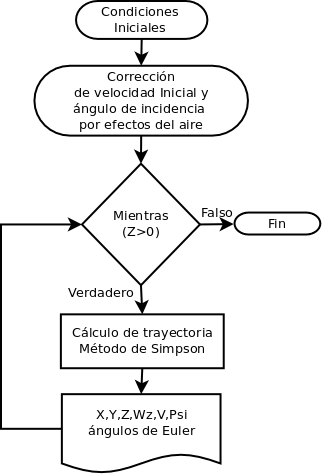
\includegraphics[scale=0.4]{imagenes/3-boomerang/diag_flu_tra.png}
		\caption{Algoritmo de cálculo de la trayectoria de vuelo del boomerang.}
		\label{fig14}
		\end{center}
		\end{figure}

\newpage
	\subsection{Interfaz de la simulación}


	El simulador de la trayectoria de vuelo del boomerang se realiza en la Interfaz Gráfica de Usuario (GUI por sus siglas en ingles) que provee $Matlab_{\textregistered}$. En la Fig. (\ref{fig15}) se muestra la intefaz gráfica creada para asignar los parámetros iniciales y observar la gráfica generada por el vuelo del boomerang.

		\begin{figure}[h]
		\begin{center}
		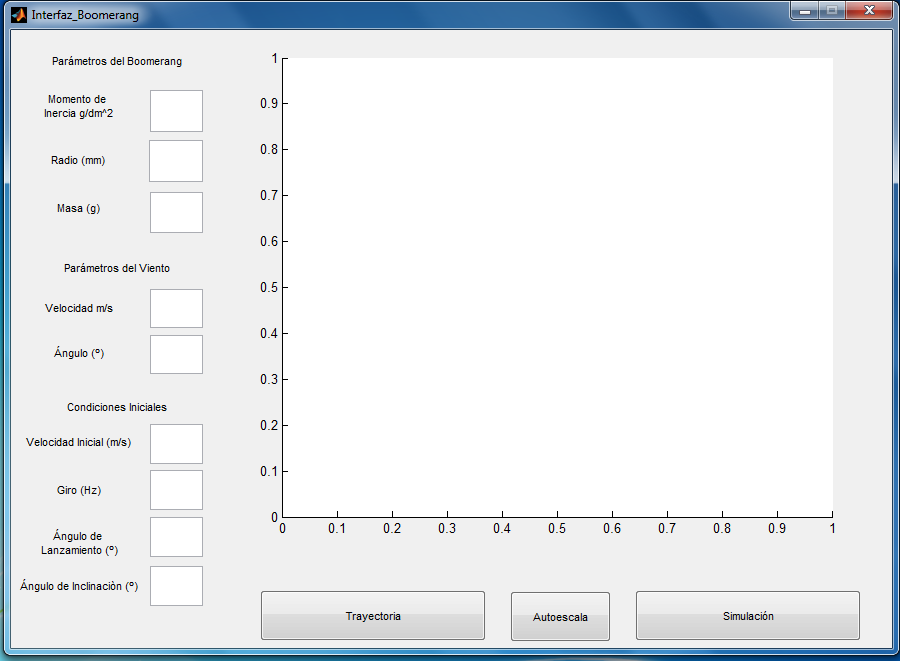
\includegraphics[scale=0.4]{imagenes/3-boomerang/GUIDE.png}
		\caption{Interfaz gráfica en la GUI de Matlab.}
		\label{fig15}
		\end{center}
		\end{figure}

\newpage
    \subsection{Simulaciones del modelo}

    Para la primer prueba del modelo se establecen los siguientes parámetros de vuelo iniciales:

		\begin{enumerate}
		\item{vel$\_$v = 0 {($\frac{m}{seg}$)}.}
		\item{vel$\_$ini = 31 {($\frac{m}{seg}$)}.}
		\item{ang$\_$v = 0 {($grados$)}.}
  		\item{ang$\_$lanzamiento $\approx$ 30 {($grados$)}.}
		\item{giro $\approx$ 10 {($Hz$)}.}
     	\item{X = 0 $m$.}
     	\item{Y = 0 $m$.}
     	\item{Z = 1.8 $m$.}
		\end{enumerate}

	En la Fig. \ref{fig16} se muestra el resultado generado por la simulación con los datos iniciales propuestos:

		\begin{figure}[h]
		\begin{center}
		\includegraphics[scale=0.45]{imagenes/3-boomerang/tray_1.png}
		\caption{Simulación 1 del modelo.}
		\label{fig16}
		\end{center}
		\end{figure}


	En la segunda prueba del modelo se agrega velocidad y ángulo de la velocidad del viento actuante en el boomerang:

		\begin{enumerate}
		\item{vel$\_$v = 5 {($\frac{m}{seg}$)}.}
		\item{vel$\_$ini = 26 {($\frac{m}{seg}$)}.}
		\item{ang$\_$v = 20 {($grados$)}.}
  		\item{ang$\_$lanzamiento $\approx$ 20 {($grados$)}.}
		\item{giro $\approx$ 10 {($Hz$)}.}
     	\item{X = 0 $m$.}
     	\item{Y = 0 $m$.}
     	\item{Z = 1.8 $m$.}
		\end{enumerate}

	De igual manera en la Fig. \ref{fig17} se muestra la trayectoria de vuelo del boomerang generada por los datos iniciales propuestos:

		\begin{figure}[h]
		\begin{center}
		\includegraphics[scale=0.45]{imagenes/3-boomerang/tray_2.png}
		\caption{Simulación 2 del modelo.}
		\label{fig17}
		\end{center}
		\end{figure}

	Finalmente se muestra una simulación con baja velocidad angular y un valor grande del ángulo de lanzamiento:

		\begin{enumerate}
		\item{vel$\_$v = 0 {($\frac{m}{seg}$)}.}
		\item{vel$\_$ini = 15 {($\frac{m}{seg}$)}.}
		\item{ang$\_$v = 0 {($grados$)}.}
  		\item{ang$\_$lanzamiento $\approx$ 60 {($grados$)}.}
		\item{giro $\approx$ 10 {($Hz$)}.}
     	\item{X = 0 $m$.}
     	\item{Y = 0 $m$.}
     	\item{Z = 1.8 $m$.}
		\end{enumerate}

	En la Fig. \ref{fig18} se muestra la trayectoria de vuelo del boomerang generada por los datos iniciales propuestos:

		\begin{figure}[h]
		\begin{center}
		\includegraphics[scale=0.45]{imagenes/3-boomerang/tray_3.png}
		\caption{Simulación 3 del modelo.}
		\label{fig18}
		\end{center}
		\end{figure}

\newpage
	Como es posible observar en la Fig. (\ref{fig16}) y en la Fig.(\ref{fig16}), al aplicarle una velocidad grande al boomerang, con ó sin velocidad del viento, el boomerang tiende a regresar cerca del punto de lanzamiento, esto debido a que los efectos presentes en el boomerang se mantienen durante el vuelo.

	En cambio en la Fig. (\ref{fig18}), el boomerang no regresa al punto de lanzamiento debido a la baja velocidad inicial con la que el boomerang fué lanzado.

	Por lo que la simulación resulta ser una aproximación a la trayectoria que genera un vuelo del boomerang.


    \section{Experimentos}


	Como lo han mostrado \cite{Hess1975}, \cite{Azuma} y \cite{Lorenz}, hasta ahora, la trayectoria de vuelo real de un boomerang se ha comparado con la obtenida en simulación a traves de videos o imagenes y dispositivos emisores de luz embarcados en este. Sin embargo esto ha sido con la intención de obtener una comparativa cualitativa, no cuantitativa.

	En este caso se ha optado por la instrumentación de un boomerang debido a lo interesante de la idea de obtener una trayectoria de vuelo cuantificada, además de que con esto será posible, posteriormente, no solo comparar los resultados reales con los obtenidos en simulación, sino buscar la parametrización del modelo.

	\subsection{Obtención y procesamiento de datos}

	Se describirán brevemente los dispositivos que conforman la unidad registradora de datos y se dará una breve explicación de las herramientas que se utilizaron para procesar estos últimos.

	\subsubsection{Dispositivos utilizados}

	\subsubsection{Unidad de medición inercial, 9DOF Razor IMU}

	Definición. Una unidad de medición inercial o IMU (del inglés Inertial Measuremente Unit) es un dispositivo electrónico que mide e informa acerca de velocidad, orientación y fuerzas gravitacionales de un aparato, usando una combinación de acelerómetros y giroscópios.

	La unidad de medición inercial 9DOF Razor IMU de Sparkfun incorpora los siguientes sensores de tres ejes:

	\begin{enumerate}
	\item {Acelerómetro de 13 bits de resolución, con rango de $\pm$ 16g, ADXL345}
	\item{Gyroscopio ITG-3200}
	\item{Magnetómetro HMC5883L}
	\end{enumerate}

	los cuales son procesados por un microcontrolador Atmega328 de 8MHz, el cual puede ser reprogramado a través del entorno de desarrollo integrado (IDE por sus siglas en inglés, Integrated development environment) de Arduino.

		\begin{figure}[h]
		\begin{center}
		\includegraphics[scale=0.3]{imagenes/3-boomerang/IMU.jpg}
		\caption{9DOF Razor IMU de SparkFun.}
		\label{fig19}
		\end{center}
		\end{figure}
\newpage
	\subsubsection{Unidad de almacenamiento de datos}

	Para llevar un registro de los datos de los sensores se utiliza un módulo de tarjetas microSD, el cual utiliza el protocolo SPI (por sus siglas en inglés, Serial Peripheral Interface) y para cuya comunicación con la IMU se utiliza la libreria SD de Arduino.

		\begin{figure}[h]
		\begin{center}
		\includegraphics[scale=0.2]{imagenes/3-boomerang/SD.png}
		\caption{Módulo de tarjetas microSD de Arduino.}
		\label{fig20}
		\end{center}
		\end{figure}

	\subsection{Algoritmo de la matriz de cosenos directores (DCM)}

	Por medio del algoritmo de la matriz de cosenos directores (DCM por sus siglas en inglés, Direction Cosine Matrix) se puede obtener la orientación de una IMU en terminos de ángulos de Euler (roll, pitch, yaw en nuestro caso) considerando compensaciones en las mediciones de los sensores (obtenidas combinando acelerómetros y gyroscopios) que permiten minimizar el error de medición.

	Los giroscopios son usados como la principal fuente de información de la orientación. Se integra la ecuación cinemática no lineal que relaciona la raza de cambio en la orientación del objeto a su taza de rotación y su orientación presente.

	Se tiene en cuenta que errores numéricos en la integración pueden violar gradualmente la restricción de ortogonalidad de la DCM, por lo que se hacen ajustes regulares en los elementos de la matriz.

	Ya que se tienden a acumular errores numéricos del gyroscopio (drift y offset) en los elementos de la DCM, se usan vectores de referencia para detectarlos y un controlador PI entre los estos errores y las entradas del gyroscopio para disiparlos más rapido de lo que se acumulan.

	En nuestro caso se utiliza un magnetómetro para detectar errores en yaw y el acelerómetro para detectar pitch y roll.

	El diagrama siguiente muestra la secuencia de procesamiento de la información de los sensores. Para profundizar en el tema, consultese \cite{Premerlany}.

		\begin{figure}[h]
		\begin{center}
		\includegraphics[scale=0.5]{imagenes/3-boomerang/DCM.jpg}
		\caption{Algoritmo DCM.}
		\label{fig24}
		\end{center}
		\end{figure}


	\subsection{Registrador de datos (Datalogger)}

Los datos de salida son almacenados en un archivo de extensión .CSV en una memoria microSD.

Se optó por implementar el algoritmo DCM en Matlab (fuera de línea), lo cual permitió deducir el periodo de muestreo a 10 ms.

Se notó que los tiempos entre adquisición de datos no se mantenían siempre en 10 ms, sino que se presentaban algunas veces periodos de 12 o incluso 20 ms. Por tanto se optó por almacenar también cada periodo de muestreo junto con los datos de los sensores en el archivo de salida.

	\subsection{Resultados del avance en la reconstrucción de la trayectoria de vuelo.}

	La trayectoria de vuelo de un boomerang se divide en orientación y posición en el espacio. La primera se obtiene utilizando el algoritmo de la matriz de cosenos directores, mientras que la segunda se obtiene al integrar dos veces los datos de aceleración del cuerpo respecto al sistema de referencia inercial.

	\subsubsection{Orientación en vuelo}

	La orientación del boomerang en vuelo es obtenida como resultado del algoritmo de la matriz de cosenos directores, el cual fue implementado en Matlab.

	La Fig. \ref{fig21} ilustra el cambio de orientación sufrido por el boomerang en instantes de tiempo $t = kT$, $k = {1, 2, 3, 4}$, de uno de los experimentos de recolección de datos inerciales realizados. Se puede notar el giro del boomerang respecto al eje Z que pasa por su centro de masa.

		\begin{figure}[h]
		\begin{center}
		\includegraphics[scale=0.25]{imagenes/3-boomerang/orientacion_boomerang.png}
		\caption{Orientación del boomerang en vuelo en cuatro instantes de tiempo consecutivos.}
		\label{fig21}
		\end{center}
		\end{figure}

	\subsubsection{Trayectoria de vuelo}

	\subsubsection{Datos de aceleración respecto al sistema inercial}

	Para obtener información de velocidad y posición respecto al sistema de referencia inercial, es necesario primero obtener la aceleración física del sensor respecto a este sistema. Para esto, es importante primero entender exactamente qué es lo que mide un acelerómetro.

	Un vector de mediciones del acelerómetro ${a}_{m}$ puede ser modelado como:

	${ a }_{ m }={ a }_{ c }-{ R }^{ c }_{ I }\left( \begin{matrix} 0 \\ 0 \\ g \end{matrix} \right)$

	donde ${a}_{c}$ es la velocidad del sensor respecto al sistema fijo al cuerpo, g es la aceleración de la gravedad, y ${R}^{c}_{I}$ es la matriz de rotación del sistema de referencial inercial al sistema fijo al cuerpo. Este modelo asume que no hay errores en la medición.

	Para estimar la velocidad y posición,  necesitamos remover la componente de gravedad de la medición, por lo cual, despejando ${a}_{b}$ tenemos:

	${ a }_{ c }={ a }_{ m }+{ R }^{ c }_{ I }\left( \begin{matrix} 0 \\ 0 \\ g \end{matrix} \right)$

	Ahora la aceleración del cuerpo debe ser rotada de tal manera que sea representada en el sistema de referenciainercial, de tal manera que pueda ser integrada para obtener velocidad y posición. Esto nos lleva a:

	${ a }_{ I }={ R }^{ I }_{ c }{ a }_{ m }+\left( \begin{matrix} 0 \\ 0 \\ g \end{matrix} \right)$


	\subsubsection{Estimados de la velocidad y posición}

	Ya que se tienen las mediciones de la aceleración del sensor respecto al sistema inercial, pueden ser integrados para obtener estimados de la velocidad y posición.

	Se utilizó el metodo de integración numérica por trapecios de la siguiente manera:

	$v\left( k \right) =v\left( k-1 \right) +h\left( a\left( k \right) +a\left( k-1 \right) \right) /2$

	y de igual manera

	$p\left( k \right) =p\left( k-1 \right) +h\left( v\left( k \right) +v\left( k-1 \right) \right) /2$

	Los periodos de muestreo h utilizados en cada iteración de las dos integrales anteriores se obtienen del archivo .CSV del registrador de datos.

	\subsubsection{Resultados}

	Utilizando la teoría mencionada anteriormente se obtuvieron los siguientes resultados, los cuales no fueron satisfactorios debido a la gran diferencia entre los datos obtenidos y lo observado durante el experimento, que se asemejaba a los resultados de simulación.

	Recuerdese que el sistema de referencia inercial del sensor esta orientado de tal manera que el eje X apunta hacia el norte magnetico de la tierra, y el Z hacia abajo, por lo que los resultados mostrados en las Figs.  \ref{fig22} y \ref{fig23} nos dicen que la componente en Z de la posición incrementa en dirección ascendente (eje Z negativo), lo cual no es correcto.

		\begin{figure}[h]
		\begin{center}
		\includegraphics[scale=0.4]{imagenes/3-boomerang/tray_vue_1.jpg}
		\caption{Trayectoria de vuelo 1.}
		\label{fig22}
		\end{center}
		\end{figure}

		\begin{figure}[h]
		\begin{center}
		\includegraphics[scale=0.4]{imagenes/3-boomerang/tray_vue_2.jpg}
		\caption{Trayectoria de vuelo 2.}
		\label{fig23}
		\end{center}
		\end{figure}
\newpage
	\subsubsection{Posibles causas de error}

	Como se mencionó, los datos obtenidos no fueron los esperados, y entre las posibles causas están:

	\begin{enumerate}
	\item Mala interpretación de los datos obtenidos,
	\item Errores en la programación,
	\item Periodo de muestreo demasiado grande y datos con mucho ruido,
	\end{enumerate}

	los cuales son los puntos a revisar en trabajo futuro.


    \section{Conclusiones}

	La solución por integración numérica de las ecuaciones de movimiento resultantes, obtenidas en el simulador, generaron trayectorias similares a las que se observan en un boomerang de retorno convencional.

	La utilización del algorimo DCM arrojó datos que muestran ser consistentes con el cambio de orientación de un boomerang durante el vuelo. Sin embargo, el giro respecto al eje Z, correspondiente al giro respecto al centro de masa del boomerang, mostró cambios demasiado pronunciados en cada periodo de muestreo (se tienen alrededor de cuatro muestras por giro), lo que significa que es necesario reducirlo algunas veces más.

	La doble integración de los datos de aceleración no arrojo información útil y será necesario revisar a detalle los puntos mencionados en la sección 4.4.2.

	La reconstrucción de la trayectoria permanece como trabajo futuro junto con la derivación de fuerzas aerodinámicas y su parametrización.


    \begin{thebibliography}{X}

\bibitem {Hess1975} \textsc{Felix Hess.} \textit{Boomerangs, Aerodynamics and Motion.} Phd. Thesis, Groningen University, Holanda, 1975.

\bibitem {barger1973} \textsc{Vernon Barger.} (1975.) \textit{The Boomerang.} \textit{En Classical Mechanics A Modern Perspective (171-178).} 2nd. Edition. University of Wisconsin:McGraw-Hill

\bibitem {Granville} \textsc{William Anthony Granville.} (2013.) \textit{Integrales Definidas.} \textit{En Cálculo Diferencial E Integral (300-306).} Limusa

\bibitem {Azuma} \textsc{Akira Azuma.} (Julio-Agosto 2004.) \textit{Flight Dynamics of the Boomerang} \textit{Journal of Guidance, Control and Dynamics,}, Vol. 27, 545-564.

\bibitem {Lorenz} \textsc{Ralph D. Lorenz.} \textit{The Boomerang.} \textit{Spinning Flight, Dynamics of Frisbees, Boomerangs, Samaras, and Skipping Stones (239-267).} Springer

\bibitem {kuleshov} \textsc{Alexander S. Kuleshov.} (2010.) \textit{A Mathematical Model of the Boomerang.} \textit{Science Direct}.

\bibitem {Dampier1729} \textsc{Dampier W.} (1729.) \textit{A new voyage round the world. Vol.1.} \textit{London}.

\bibitem {Premerlany} \textsc{William Premerlani and Paul Bizard.} (2009.) \textit{Direction Cosine Matrix IMU: Theory}

\end{thebibliography}
%
% \end{document}


    \chapter{Dinámica Agro-Socio-Ambiental en la conservación de la biodiversidad en México mediante la regulación de la calidad de la Matriz Agrícola}
    \paragraph{Alan Osorio Orduña, Sergio Naude Citalán}
    
% \renewcommand{\tablename}{Tabla}
% \renewcommand{\listtablename}{Índice de Tablas}
% \renewcommand{\listfigurename}{Índice de Figuras}
% \begin{titlepage}
% \begin{center}
% \includegraphics[width=0.15\textwidth]{imagenes/cinvestav}~\\[1cm]
%
% \textsc{\LARGE CINVESTAV-IPN}\\[1.5cm]
%
% \textsc{\Large Proyecto Final Modelado y Simulación}\\[0.5cm]
%
% % Title
% \HRule \\[0.4cm]
% { \huge \bfseries Dinámica Agro-Socio-Ambiental en la conservación de la biodiversidad en México mediante la regulación de la calidad de la Matriz Agrícola\\[0.4cm] }
%
% \HRule \\[1.5cm]
%
% % Author and supervisor
% \noindent
% \begin{minipage}{0.4\textwidth}
% \begin{flushleft} \large
% \emph{Autores:}\\
% \begin{itemize}
% \item[$\bullet$] Alan Osorio Orduña
% \item[$\bullet$] Sergio Naude Citalán
% \end{itemize}
% \end{flushleft}
% \end{minipage}%
% \begin{minipage}{0.4\textwidth}
% \begin{flushright} \large
% \emph{Profesor:} \\
% D. en C. Juan Carlos Martínez García
% \end{flushright}
% \end{minipage}
% \vfill
% % Bottom of the page
% %{\large \today}
% \end{center}
% \end{titlepage}
% %\newcommand{\HRule}{\rule{\linewidth}{0.15cm}}

%\pagenumbering{Roman} % para comenzar la numeración de paginas en números romanos
\section*{Resumen}
Hoy en día las reservas naturales están siendo afectadas por la actividad humana. La producción agrícola no planificada adecuadamente, genera destrucción del hábitat alterando los ecosistemas, de tal forma que en ocasiones resulta en un daño irreversible.    \\

Disminuir el impacto ambiental provocado por las zonas de cultivo cercanas a reservas naturales sin interrumpir la producción agrícola, es una de las prioridades en diferentes partes del mundo.\\

En base a estudios que sean realizados en los últimos años se piensa que la matriz agrícola es de vital importancia. Es útil ver de manera gráfica y numérica los efectos que el hombre causa en la naturaleza. Razón por la cual se recopilo información de diferentes fuentes, todas relacionadas con el cultivo de café en Chiapas. Los datos recopilados fueron almacenados en una base de datos, para después ser utilizados para el modelo matemático realizado con cadenas markovianas. A partir de los resultados obtenidos en el modelo se describe la proyección a futuro de la calidad de la matriz. Los parámetros considerados para determinar la calidad de la matriz fueron de distintos ámbitos, desde flora y fauna del lugar, hasta métodos de cultivo y compuestos de plaguicidas y fertilizantes. \\

Con este proyecto se pretende configurar los parámetros necesarios para cambiar el estado de la calidad de  una matriz a otro, o por el contrario mantenerlo en un tiempo determinado.\\

Se realizaron programas de software para visualizar y conocer el la calidad de la matriz agrícola de las zonas de cultivos con respecto a las especies que habitan en los alrededores en un tiempo especificado.\\

Para la creación y depuración del programa se usó un compilador orientado a agentes, el cual permitió ver la interacción de las especies animales con el medio.
% \newpage
% \tableofcontents % indice de contenidos
% %\addcontentsline{toc}{chapter}{Indice de contenidos} % si queremos que aparezca en el índice
% %\newpage
% %\thispagestyle{empty}
% %\listoffigures % indice de figuras
% %\addcontentsline{toc}{chapter}{Índice de Figuras} % para que aparezca en el indice de contenidos
% \newpage
% \thispagestyle{empty}
% %\listoftables % indice de tablas
% %\addcontentsline{toc}{chapter}{Índice de Tablas} % para que aparezca en el indice de contenidos
% %\newpage
% %\thispagestyle{empty}
% %\newpage


\section{Introducción}
El crecimiento urbano propicia cambios en los espacios circundantes, tales como la pérdida de áreas agrícolas y forestales a favor de los ambientes urbanizados, y cambios en las estructuras socioeconómicas relacionadas con el manejo y propiedad de la tierra.\\

Chiapas es un estado con un fuerte crecimiento pero que aún mantiene áreas forestales, que cuentan con esquemas de protección de sus bosques.\\

El efecto del crecimiento urbano es complejo y no unidireccional, pues representa una fuerte presión para el cambio de uso del suelo, pero también ha permitido la reactivación de actividades agrícolas de bajo impacto y la revalorización de las áreas forestales.\\

Chiapas es conocido por su alta diversidad de especies de mamíferos, sin embargo, en la entidad grandes extensiones de hábitats naturales han sido modificados a zonas agrícolas, lo cual se cree que disminuye la riqueza de especies.\\

Por ello, el presente trabajo tiene como objetivo determinar la riqueza de suelo en zonas agrícolas del estado de Chiapas, particularmente en las que se cultiva café. Se recopiló información de las especies de flora y fauna de la región en bases de datos del gobierno estatal y federal, así como en colecciones de literatura científicas nacionales e internacionales.

\section{Objetivos}

\begin{itemize}
\item[$\bullet$] Descripción de la dinámica espacio-temporal de los factores agro-socio-ambientales relacionados con los sistemas agrícolas que impactan la calidad de la matriz agroecológica. Mediante el empleo de dinámicas Markovianas para la descripción de la evolución de la matriz agro-ecológica y considerando la interacción de territorios aledaños mediante dinámicas de agentes.
\item[$\bullet$] Desarrollo de un simulador computacional capaz de analizar mediante sistemas de información geográfica y bases de datos disponibles el escenario del impacto de distintos tipos de manejo agrícola en diversos contextos socio- ambientales en la dinámica espacio-temporal de la matriz.
\end{itemize}

\section{Marco Teórico}
\subsection{Cadenas de Markov}
Se conoce como cadena de Márkov a un tipo especial de proceso estocástico discreto en el que la probabilidad de que ocurra un evento depende solamente del evento inmediatamente anterior. Si se conoce la historia del sistema hasta su instante actual, su estado presente resume toda la información relevante para describir en probabilidad su estado futuro.\\

Si el estado $X_n$ y los estados previos $X_1, \dots,X_{n-1}$ son conocidos. La probabilidad del estado futuro $X_{n+1}$. No depende de los estados anteriores $X_1,\dots,X_{n-1}$. Solamente depende del estado $X_n$.\\

Es decir,

\begin{itemize}
\item[$\bullet$] Para $n = 1, 2,\dots$ y
\item[$\bullet$] Para cualquier sucesión de estados $s_1,\dots,s_{n+1}$.
\end{itemize}

\begin{multline}
    P(X_{n+1} = s_{n+1} | X_1 = s_1, X_2 = s_2,\dots, X_n = s_n ) \\ =  P(X_{n+1} = s_{n+1} | X_n = s_n)
\end{multline}

\subsection{Matriz de transición}
En matemáticas, una matriz de Markov es una matriz utilizada para describir las transiciones en una cadena de Markov. Existen varias definiciones y tipos de matriz estocástica:

\begin{itemize}
\item Una matriz estocástica derecha es una matriz cuadrada cada una de cuyas filas está formada por números reales no negativos, sumando cada fila 1.
\item Una matriz estocástica izquierda es una matriz cuadrada cada una de cuyas columnas está formada por números reales no negativos, sumando cada columna 1.
\item Una matriz doble estocástica es una matriz cuadrada donde todos los valores son no negativos y todas las filas y columnas suman 1.
\end{itemize}

Un proceso de Markov en que el sistema posee $n$ estados posibles, dados por los números $1, 2, 3,\dots., n$. Denotemos $p_{ij}$  a la probabilidad de que el sistema pase al estado $j$ después de cualquier ensayo en donde su estado era $i$ antes del ensayo. Los números $p_{ij}$  se denominan probabilidades de transición y la matriz $n\times n$  $P = (p_{ij})$ se conoce como matriz de transición del sistema.\\

La suma $1\dots p_{i1} + p_{i2} + p_{in} = 1$. Esta suma representa la probabilidad de que el sistema pase a uno de los estados $1, 2,\dots, n$ dado que empieza en el estado $i$. Ya que el sistema ha de estar en uno de estos n estados, la suma de probabilidades debe ser igual a 1. Esto significa que los elementos en cualquier renglón de la matriz de transición deben sumar $1$.  Cada elemento $p_{ij}\geq0$.\\

De la misma manera, puede definirse un vector estocástico como un vector cuyos elementos están formados por números reales no negativos que suman 1. Así, cada fila (o columna) de una matriz estocástica es un vector de probabilidad, también llamados vectores estocásticos.

\section{Simulación}
Dentro de la simulación son usados dos programas principalmente. El primero de ellos es Matlab con una interfaz gráfica, el segundo es el programa de desarrollo de ambientes Netlogo.\\

La interfaz gráfica implementada en Matlab permite ingresar los datos de la matriz de transición. Cada elemento de la matriz y el vector de condiciones iniciales son introducidos manualmente por el usuario. Después mediante un algoritmo de iteraciones entre el vector de condiciones iniciales y la propia matriz de transición, se obtiene un vector de salida. Éste último nos indica en qué tipo de clasificación se encuentra la matriz.\\

Primero se introducen las condiciones iniciales en forma de vector fila. Dichas condiciones indican la calidad de la matriz en un inicio, en escala de 0 a 1, siendo 1 excelente calidad. En base a diversas propiedades con las que cuenta la matriz es como se le asignan las componentes al vector. En el presente trabajo los factores considerados fueron:

\begin{itemize}
\item Tipo de cultivo.
\item Fertilizantes y/o plaguicidas.
\item Calidad de sombra.
\end{itemize}

La Figura \ref{fig:1} muestra la interfaz en Matlab

\begin{center}
\includegraphics[scale=0.45]{imagenes/4-agricola/1.png}
\captionof{figure}{Interfaz gráfica- Matriz de Markov}
\label{fig:1}
\end{center}

La matriz de transición nos condensa las probabilidades de un estado a otro. A través de ésta matriz se puede observar el comportamiento representado por una cadena de Markov. Es decir, las propiedades de cambio entre los estados de la matriz agrícola.\\

Finalmente el periodo (en años) acota la escala de tiempo en la que se evalúa la matriz. Limitado por la información disponible, la proyección sólo se puede hacer máximo a 10 años.\\

El vector de condiciones iniciales es el siguiente:
$$\left[\begin{array}{ccc}
0{.}1&0{.}5&0{.}9
\end{array}\right]$$
La matriz de transición fijada es la siguiente:

\begin{align*}
\left[\begin{array}{ccc}
0{.}3&0{.}6&0{.}7
\end{array}\right]\\
\left[\begin{array}{ccc}
0{.}1&0{.}3&0{.}8
\end{array}\right]\\
\left[\begin{array}{ccc}
0{.}4&0{.}6&0{.}6
\end{array}\right]
\end{align*}

El programa en Netlogo muestra de manera gráfica la interacción de la matriz agrícola con especies animales. Además presenta el impacto que tienen distintos métodos de cultivo en la población de la fauna silvestre. La Figura \ref{fig:2} muestra el programa de Netlogo en ejecución.

\begin{center}
\includegraphics[scale=0.45]{imagenes/4-agricola/2.PNG}
\captionof{figure}{Interfaz en Netlogo}
\label{fig:2}
\end{center}

\section{Manual de software de simulación la calidad de la matriz agrícola de café}
\begin{enumerate}
\item Se seleccionan los parámetros de la zona agrícola.

\item Tipo de diseño, sombra, toxicidad y acumulativos.

\item Se da clic en ajustar para que muestre la zona agrícola con los parámetros deseados.

\item Se selecciona el animal con el que se pretenda visualizar como atravesara la zona agrícola con los parámetros descritos anteriormente.

\item Se presiona el botón ``preparar'' para ajustar el entorno y las variables que van estar interactuando durante el paso de la especie animal por la zona agrícola.

\item Se presiona el botón ``paso'' para que avancen cierta cantidad de espacio los animales por la zona agrícola hasta que salgan de ella.

\item Se colocan los nuevos parámetros así como la cantidad de años que a la que se quiere visualizar como se verá la matriz a tiempo futuro con los nuevos parámetros.
\end{enumerate}

\section{Conclusiones}
Se prueba la importancia de la calidad de la matriz agrícola en su entorno (en este caso es específicamente la relacionada con el cultivo de café).\\

Se visualiza de manera gráfica y numérica el impacto de la matriz con su alrededor en un tiempo finito a través de la modificación de ciertos parámetros.\\

Se encuentra la ponderación de los parámetros que puede modificar  de manera directa el hombre sobre la matriz agrícola en las zonas de cultivo de café.\\

Se logra visualizar los rangos de valores que deben tener los parámetros para reducir los daños generados por el hombre mientras realiza una actividad agrónoma,  en este caso el cultivo de café.

\bibliographystyle{ieeetr} \nocite{*}
\bibliography{xbiblioteca} %bibliografía.


    \chapter{Interacción entre el Bienestar Psicológico y el Paisaje Sonoro}
    \paragraph{Ing. Concepción Jazmín Suárez Polo, Ing. Milcom Elijack Peregrina Ochoa}
    
% \documentclass{article}
% \usepackage{amsfonts}

%%%%%%%%%%%%%%%%%%%%%%%%%%%%%%%%%%%%%%%%%%%%%%%%%%%%%%%%%%%%%%%%%%%%%%%%%%%%%%%%%%%%%%%%%%%%%%%%%%%%%%%%%%%%%%%%%%%%%%%%%%%%%%%%%%%%%%%%%%%%%%%%%%%%%%%%%%%%%%%%%%%%%%%%%%%%%%%%%%%%%%%%%%%%%%%%%%%%%%%%%%%%%%%%%%%%%%%%%%%%%%%%%%%
%TCIDATA{OutputFilter=LATEX.DLL}
%TCIDATA{Version=5.50.0.2953}
%TCIDATA{<META NAME="SaveForMode" CONTENT="1">}
%TCIDATA{BibliographyScheme=Manual}
%TCIDATA{Created=Sunday, December 14, 2014 13:08:08}
%TCIDATA{LastRevised=Sunday, December 14, 2014 18:02:07}
%TCIDATA{<META NAME="GraphicsSave" CONTENT="32">}
%TCIDATA{<META NAME="DocumentShell" CONTENT="Scientific Notebook\Blank Document">}
%TCIDATA{CSTFile=Math with theorems suppressed.cst}
%TCIDATA{PageSetup=72,72,72,72,0}
%TCIDATA{AllPages=
%F=36,\PARA{038<p type="texpara" tag="Body Text" >\hfill \thepage}
%}


% \newtheorem{theorem}{Theorem}
% \newtheorem{acknowledgement}[theorem]{Acknowledgement}
% \newtheorem{algorithm}[theorem]{Algorithm}
% \newtheorem{axiom}[theorem]{Axiom}
% \newtheorem{case}[theorem]{Case}
% \newtheorem{claim}[theorem]{Claim}
% \newtheorem{conclusion}[theorem]{Conclusion}
% \newtheorem{condition}[theorem]{Condition}
% \newtheorem{conjecture}[theorem]{Conjecture}
% \newtheorem{corollary}[theorem]{Corollary}
% \newtheorem{criterion}[theorem]{Criterion}
% \newtheorem{definition}[theorem]{Definition}
% \newtheorem{example}[theorem]{Example}
% \newtheorem{exercise}[theorem]{Exercise}
% \newtheorem{lemma}[theorem]{Lemma}
% \newtheorem{notation}[theorem]{Notation}
% \newtheorem{problem}[theorem]{Problem}
% \newtheorem{proposition}[theorem]{Proposition}
% \newtheorem{remark}[theorem]{Remark}
% \newtheorem{solution}[theorem]{Solution}
% \newtheorem{summary}[theorem]{Summary}
% \newenvironment{proof}[1][Proof]{\noindent\textbf{#1.} }{\ \rule{0.5em}{0.5em}}
% \input{tcilatex}
%
% \begin{document}


\begin{center}
CENTRO DE INVESTIGACIONES AVANZADAS DEL INSTITUTO POLIT\'{E}CNICO NACIONAL

DEPARTAMENTO DE CONTROL AUTOM\'{A}TICO

MAESTR\'{I}A EN CIENCIAS EN CONTROL AUTOM\'{A}TICO

REPORTE FINAL DE PROYECTO

\textbf{INTERACCI\'{O}N ENTRE EL BIENESTAR PSICOL\'{O}GICO Y EL PAISAJE
SONORO.}

ING. CONCEPCI\'{O}N JAZM\'{I}N SU\'{A}REZ POLO

ING. MILCOM ELIJACK PEREGRINA OCHOA

ASESOR: DR. JUAN CARLOS MART\'{I}NEZ GARC\'{I}A

\bigskip

DICIEMBRE 2014

\bigskip
\end{center}

\textbf{Indice general. }

Resumen \qquad 2

Abstract\qquad 2

1. Introducci\'{o}n\qquad 2

2. Cronograma\qquad 3

3. Estado del arte\qquad 3

3.1 Surgimiento y desarrollo del concepto de paisaje sonoro.\qquad 3

3.2 Caracter\'{\i}sticas del paisaje sonoro.\qquad 3

3.3 An\'{a}lisis del paisaje sonoro.\qquad 4

3.4 Estructura del paisaje sonoro.\qquad 5

3.5 Caracter\'{\i}sticas estructurales para el an\'{a}lisis de paisajes
sonoros.\qquad 5

4. Entrevista.\qquad 6

5. Parte Experimental.\qquad 8

5.1 Equipo de grabaci\'{o}n.\qquad 8

5.2 Grabaci\'{o}n de campo.\qquad 9

5.2.1 Paisaje sonoro natural y paisaje sonoro con elemento humano.\qquad 9

5.2.2 Paisaje sonoro urbano.\qquad 10

5.3 Edici\'{o}n y an\'{a}lisis de las grabaciones.\qquad 10

6. Dise\~{n}o de la Red Perceptr\'{o}n Multicapa con algoritmo

supervisado Backpropagation tipo gradiente.\qquad 12

6.1 Acondicionamiento de datos.\qquad 17

6.2 Entrenamiento de la red neuronal.\qquad 18

6.3 Modo de operaci\'{o}n de la aplicaci\'{o}n.\qquad 23

Conclusiones.\qquad 24

Referencias.\qquad 24

Bibliograf\'{\i}a consultada.\qquad 24

\textbf{\'{I}ndice de figuras y tablas}

Figura 1. Grabadora Tascam DR40\qquad 8

Figura 2. Aud\'{\i}fonos Sennheiser hd 205\qquad 8

Figura 3. Grabadora Tascam DR40 montada en tr\'{\i}pode y con
antiviento\qquad 9

Figura 4. Espectrograma antes y despu\'{e}s de correcciones\qquad 11

Figura 5. An\'{a}lisis de espectro en frecuencia paisaje natural, natural
con\qquad 12

elemento humano y urbano respectivamente\qquad 12

Figura 6. Datos del espectrograma.\qquad 12

Figura 7. Representaci\'{o}n de una Neurona\qquad 14

Figura 8. Funci\'{o}n sigmoidea\qquad 15

Figura 9. Espectro analizado por Audacity\qquad 18

Figura 10. Organizaci\'{o}n de los datos en hojas de c\'{a}lculo\qquad 18

Figura 11. Gr\'{a}fica en Matlab de los datos de entrenamiento\qquad 19

Figura 12. Patrones de entrenamiento\qquad 19

Figura 13. Hipermatriz de capas de la red neuronal\qquad 13

Figura 14. Matriz de Bias de la red neuronal\qquad 20

Figura 15. Resultado para 500 \'{e}pocas\qquad 21

Figura 16. Resultado para 600 \'{e}pocas\qquad 21

Figura 17. Resultado para 800 \'{e}pocas\qquad 22

Figura 18. Aplicaci\'{o}n standalone\qquad 23

Tabla 1. Cronograma de actividades.\qquad 3

Tabla 2. Rangos de sonido de la OMS\qquad 22

\textbf{Resumen }

En el presente Proyecto, se realizar\'{o}n grabaciones de campo en tres
entornos sonoros distintos, catalogados como paisaje sonoro natural, natural
con elemento humano y urbano. A partir de las grabaciones se procedi\'{o} a
un tratamiento digital de la se\~{n}ales, los datos obtenidos se utilizaron
como referentes para el correspondiente entrenamiento de una red neuronal
basada en el modelo de Retro-propagaci\'{o}n que realiza una m\'{e}trica
espacial y temporal de la calidad de un paisaje sonoro, adem\'{a}s de
obtenerse la flexibilidad de caracterizar aquellos paisajes sonoros nocivos
y su relaci\'{o}n con el malestar psicol\'{o}gico.

\textbf{Abstract }

In the current project, field recordings were performed in three different
sound environments, categorized as natural soundscape, natural soundscape
with human element and urban soundscape. From the recordings we proceeded to
a digital processing of signals, data obtained were used as references for
the corresponding back propagation neural network training, which performs a
spatial and temporal soundscape quality metric, plus we obtained the
flexibility to characterize harmful soundscapes and its relationship to
psychological distress.

\textbf{1. Introducci\'{o}n}

Contrariamente a nuestra percepci\'{o}n visual, no podemos renunciar al
sentido del o\'{\i}do, carecemos de \textquotedblleft parpados
auditivos\textquotedblright . Nuestra escucha es adem\'{a}s
\textquotedblleft omnidireccional\textquotedblright , consciente o
inconscientemente, la escucha constituye a menudo nuestro primer
acercamiento y modo de comprensi\'{o}n del entorno. Principlamente nos
servimos de ella como de un \textquotedblleft radar\textquotedblright\ que
nos informa de cuanto nos rodea y que nos indica en que hemos de fijar
nuestra atenci\'{o}n, al tiempo que nos permite descartar muchas otras
fuentes de informaci\'{o}n [1].

Los sonidos que se escuchan hoy en d\'{\i}a en cualquier ciudad son muy
distintos de aquellos que pod\'{\i}an escucharse haces algunos a\~{n}os,
todo ellos debido al r\'{\i}tmico cambio mayormente acentuado a partir de la
Revoluci\'{o}n Industrial. Muchos de los sonidos naturales del propio
entorno se han visto opacados o desaparecidos del paisaje sonoro actual, la
respuesta de los habitantes de un espacio con contaminaci\'{o}n ac\'{u}stica
se traduce en malestares psicol\'{o}gicos entre otras cosas. Hoy en d\'{\i}a
con el desarrollo de la ciencia y tecnolog\'{\i}a es posible explorar,
estudiar y disfrutar los sonidos de estos tiempos, as\'{\i} como
herramientas para el an\'{a}lisis de un paisaje sonoro partiendo de su
descomposici\'{o}n en elementos. Y es justamente esta caracter\'{\i}stica la
que nos permite desarrollar herramental para describir interacciones y
mejorar la calidad ac\'{u}stica del ambiente.

\textbf{2. Cronograma.}

$%
\begin{array}{cc}
\text{\textbf{Semana}} & \text{\textbf{Actividades}} \\
\text{1} & \text{Entrevistas} \\
\text{2} & \text{Elecci\'{o}n de lugares y objetos agrabar} \\
\text{3} & \text{Gesti\'{o}n de permisos de grabaci\'{o}n} \\
\text{4} & \text{Grabaciones en campo } \\
\text{5} & \text{Grabaciones en campo} \\
\text{6} & \text{Edici\'{o}n de los archivos y an\'{a}lisis en el dominio de
la frecuencia} \\
\text{7} & \text{Extracci\'{o}n de los elementos caracter\'{\i}sticos} \\
\text{8} & \text{Dise\~{n}o de una red neuronal artificial por algoritmo de
retropropagaci\'{o}n} \\
\text{9} & \text{Entrenamiento de la red neuronal} \\
\text{10} & \text{Construcci\'{o}n de paisajes sonoros} \\
\text{11} & \text{Construcci\'{o}n de aplicaci\'{o}n}%
\end{array}%
$

Tabla 1. Cronograma de actividades.

\textbf{3. Estado del arte}

\textbf{\qquad 3.1 Surgimiento y desarrollo del concepto de paisaje sonoro.}

El t\'{e}rmino paisaje sonoro deriva de paisaje terrestre [N. del T.: en ingl%
\'{e}s "soundscape" deriva de "landscape"]. El paisaje sonoro hace
referencia a cualquier ambiente ac\'{u}stico, ya sea natural, urbano, o
rural, que este formado por tres componentes: la biofon\'{\i}a: sonidos biol%
\'{o}gicos no humanos que se producen en una ambiente dado, la geofon\'{\i}%
a: sonidos ni humanos ni biol\'{o}gicos, como el efecto del viento, el agua
o el clima, y la antrofon\'{\i}a: el ruido que produce el ser humano por
cualquier medio [5]. Por lo tanto, el medio ambiente sonoro (o paisaje
sonoro), que es la suma de la totalidad de sonidos dentro de un \'{a}rea
definida, es un reflejo \'{\i}ntimo de -entre otros- las condiciones
sociales, pol\'{\i}ticas, tecnol\'{o}gicas y naturales del \'{a}rea. Cambios
en las mencionadas condiciones implican cambios en el medio ambiente sonoro
[4].

El compositor canadiense R. Murray Schafer us\'{o} los t\'{e}rminos paisaje
sonoro ("soundscape") y ecolog\'{\i}a ac\'{u}stica para describir cr\'{\i}%
ticamente nuestro medio ambiente como un campo humano-ecol\'{o}gico ubicado
entre "el sonido y el ruido". A partir de all\'{\i} desarroll\'{o} la idea
de una disciplina futurista, con claras influencias de la bauhaus$^{1}$, el
dise\~{n}o ac\'{u}stico. Su idea era juntar compositores contempor\'{a}neos
con arquitectos, dise\~{n}adores de productos e ingenieros a fin de
desarrollar sonidos para los innumerables objetos de nuestra vida cotidiana
[6].

Por su parte el compositor Barry Truax diferencia lo que es un medio
ambiente s\'{o}nico de un paisaje sonoro. Para el, el primero comprende toda
la energ\'{\i}a ac\'{u}stica en un contexto dado, mientras que el segundo es
la comprensi\'{o}n de ese medio ambiente s\'{o}nico para aquellos que viven
en \'{e}l y lo est\'{a}n creando continuamente.$^{2}$ Para Truax, la audici%
\'{o}n es algo fundamental, ya que constituye la interface entre el
individuo y el medio ambiente, por lo tanto el paisaje sonoro es el sistema
resultante de la suma de estos dos componentes. Para Abraham Moles el
paisaje sonoro es una secuencia corta de entre 4 y 8 segundos que incluye
una idea compuesta por uno o varios signos que nos describen algo que est%
\'{a} sucediendo (ideoscena).

\textbf{\qquad 3.2 Caracter\'{\i}sticas del paisaje sonoro.}

\textquotedblleft La vida cotidiana tiene una banda sonora. Si no la
escuchamos, es porque ya estamos acostumbrados a o\'{\i}rla.%
\textquotedblright , nos dice el music\'{o}logo Ram\'{o}n Pelinski.

Existen una multitud de sonidos a nuestro alrededor, sonidos propios de la
naturaleza y aquellos generados cotidianamente en cada uno de nuestros
quehaceres. Sin embargo pocos son los que realmente escuchan estos sonidos,
estos paisajes que describen el lugar en el que vivimos y el entorno en el
que nos movemos [7].

De acuerdo con Schafer, las cualidades de un paisaje sonoro son:
\textquotedblleft sonidos t\'{o}nicos\textquotedblright\ (keynote sounds),
un conjunto de rasgos de identidad constituido por cuanto o\'{\i}mos de
forma distra\'{\i}da, sin atenci\'{o}n particular pues forman un continuo,
un fondo sonoro al que estamos plenamente habituados, $^{4}$
\textquotedblleft sonidos se\~{n}ales\textquotedblright , los sonidos que
existen en un primer plano y que son escuchados de manera consciente. Son m%
\'{a}s que figuras de fondo y la mayor\'{\i}a de veces representan c\'{o}%
digos; \textquotedblleft sonidos importantes\textquotedblright\
(soundmarks), esto es, los sonidos que los individuos identifican como
sonidos claves de su comunidad. Murray habla tambi\'{e}n de sonidos que se
manifiestan como terreno (ground), que interpreto como sonidos fondo
(background), y de figuras que se manifiestan en un primer plano
(foreground),$^{5}$, as\'{\i} como de un tercer nivel llamado campo (field),
que es el lugar desde el cual se escucha el paisaje sonoro.

En cuanto a paisajes sonoros urbanos tomaremos la definici\'{o}n de Ricardo
Atienza, de acuerdo con \'{e}l, cada espacio urbano posee unos rasgos
sonoros caracter\'{\i}sticos que nos comunican de sus cualidades espaciales,
de las temporalidades y de los usos que lo habitan. Tales rasgos constituyen
su identidad ordinaria, cotidiana. El continuo sonoro de las ciudades no es
un \textquotedblleft ruido\textquotedblright\ neutro y arbitrario; el
estudio de sus atributos compositivos constituye un an\'{a}lisis cualitativo
de las diferentes configuraciones urbanas [1].

No podemos comprender la identidad de un lugar sin conocer primero de que
modo es habitado, recorrido y practicado un espacio. An\'{a}logamente, la
identidad de cada persona estar\'{a} vinculada en gran medida a los espacios
que habite. Esta doble interacci\'{o}n nos permite comprender la identidad
de un lugar como la expresi\'{o}n cualitativa de un espacio a trav\'{e}s de
sus modos de vida caracter\'{\i}sticos. Podriamos decir entonces que, todo
fen\'{o}meno de identidad no es sino el resultado de la tensi\'{o}n que se
establece entre una memoria sonora y una escucha futura o proyectada o bien
tratarse de un proceso din\'{a}mico tanto en las periodicidades c\'{\i}%
clicas de cada d\'{\i}a o de cada estaci\'{o}n, como en la progresiva evoluci%
\'{o}n social y espacial de un lugar [1].

\textbf{\qquad 3.3 An\'{a}lisis del paisaje sonoro.}

Murray Schafer propone varios par\'{a}metros para el an\'{a}lisis de objetos
sonoros que forman parte de los paisajes sonoros:

1. Escuchado con claridad; claridad moderada; poca claridad; sobre el
ambiente general.

2. Ocurrencia aislada; repetida; parte de un contexto m\'{a}s grande o
mensaje.

3. Factores de medioambiente: sin reverberaci\'{o}n, poca reverberaci\'{o}n,
larga reverberaci\'{o}n, eco, flujo, desplazamiento.

A su vez Abraham Moles propone otros rasgos significativos del medio
ambiente sonoro, de los cuales algunos de los m\'{a}s relevantes para este
proyecto son los siguientes:

1. Numero relativo de elementos. Densidad global de los acontecimientos.

2. Complejidad del conjunto de los elementos: n\'{u}mero y variedad de las
relaciones.

3. Relaci\'{o}n entre la masa de los elementos \textquotedblleft
cercanos\textquotedblright\ y la de los elementos \textquotedblleft
lejanos\textquotedblright\ (noci\'{o}n de \textquotedblleft primer
plano\textquotedblright).$^{6}$

El artista sonoro e investigador Manuel Rocha Iturbide, en su articulo
\textquotedblleft Estructura y percepci\'{o}n psicoac\'{u}stica del paisaje
sonoro electroac\'{u}stico\textquotedblright\ a\~{n}ade dos aspectos m\'{a}s
que no fueron abordados por Schafer y Moles, estos son:

1. La escucha lineal en oposici\'{o}n a la escucha no lineal de un paisaje
sonoro determinado. Por el termino lineal se refiere a una escucha en la que
no podemos concentrarnos y seguir \qquad\ \ el transcurso de los eventos, y
por no lineal, a una escucha en la que nuestra atenci\'{o}n va
constantemente de un lugar a otro, sin permitirnos asimilar o percibir
continuidad.

2. El car\'{a}cter continuo o discontinuo en la estructura del paisaje
sonoro. Puede haber paisajes sonoros esencialmente continuos pero con
elementos discontinuos, o viceversa.

\textbf{\qquad 3.4 Estructura del paisaje sonoro.}

Schafer define dos caracter\'{\i}sticas importantes para el an\'{a}lisis de
paisajes sonoros, los paisajes sonoros Hi-Fi y Low-Fi. En los primeros,
\textquotedblleft los sonidos se sobreponen menos frecuentemente, hay
perspectiva (amplitud de fondo)\textquotedblright\ $^{7}$. Estos paisajes se
manifiestan m\'{a}s en el campo que en la ciudad. En los segundos, Lo-Fi,
los distintos planos se empastan unos con otros, y es muy dif\'{\i}cil
discernir figuras o fondos claros. Estos paisajes son t\'{\i}picos de las
grandes urbes debidas sobre todo al ruido del tr\'{a}fico en las calles,
perif\'{e}ricas y carreteras.$^{8}$

Otros dos t\'{e}rminos que usa Schafer son gesto y textura. El primero se
refiere a una figura que constituye un \'{u}nico y distinguible evento, y el
segundo a un agregado, el efecto de manchas de imprecisi\'{o}n an\'{a}rquica
y de acciones conflictivas. En cuanto a la textura, Schafer realiza la
siguiente clasificaci\'{o}n: textura del medio ambiente escuchado: hi-fi,
low-fi, natural, humano y tecnol\'{o}gico. Por su parte, Truax habla tambi%
\'{e}n de la densidad como un posible par\'{a}metro descriptivo.

\textbf{\qquad 3.5 Caracter\'{\i}sticas estructurales para el an\'{a}lisis
de paisajes sonoros. }

El investigador Manuel Rocha en su mismo articulo identifica cuatro tipos de
paisajes sonoros, para este proyecto de investigaci\'{o}n unicamente se
utilizo \textit{paisajes sonoros naturales}, \textit{paisajes sonoros
naturales con elemento humano} y \textit{paisajes sonoros urbano}s para
clasificar los entornos sonoros de estudio.

El paisaje sonoro natural corresponde a un entorno donde principalmente se
detecta sonidos del agua, del viento, sinfon\'{\i}as pajariles, sonidos de
insectos, etc. El paisaje sonoro natural con elemento humano, el cual se
utilizo en el proyecto para clasificar espacios naturales en los que adem%
\'{a}s de los sonidos propios de un paisaje natural podemos encontrarnos con
sonidos de caracter discontinuo propios de la intervenci\'{o}n del humano. \
El paisaje sonoro urbanos presenta una mayor riqueza de fuentes sonoras
respecto a los anteriores pues en el podemos encontrar diferentes sonidos,
ya sean humanos (voces, pasos, etc.), mec\'{a}nicos (tr\'{a}fico vehicular, m%
\'{a}quinas, etc.) en incluso sonidos naturales (p\'{a}jaros, fuentes de
agua, etc.), los cuales contribuyen a la diferenciaci\'{o}n de m\'{u}ltiples
paisajes sonoros urbanos, los cuales coexisten y, en m\'{u}ltiples casos, se
combinan dentro la aglomeraci\'{o}n urbana.

Importante mencionar que de acuerdo con el investigador \ Manuel Rocha, el
tiempo m\'{\i}nimo para poder comprender la estructura de un paisaje sonoro,
as\'{\i} como para analizar su complejidad, es de unos 40 segundos. La decisi%
\'{o}n respecto a caminar y como girar el campo est\'{e}reo de los micr\'{o}%
fonos durante el proceso de grabaci\'{o}n, son decisiones de car\'{a}cter
estructural y de composici\'{o}n activa consciente.

\textbf{4. Entrevista.}

La presente entrevista se realiz\'{o} al experto en paisaje sonoro, grabaci%
\'{o}n de campo y experimentaci\'{o}n sonora Enrique Maraver Aguirre.

\textbf{1. Comentenos un poco sobre usted. }

- \textit{Mi nombre es Enrique Maraver Aguirre, nacido en el Distrito
Federal. Egresado del Instituto Politecnico Nacional como Ingeniero Quimico
Industrial, posteriormente me involucre en la cuesti\'{o}n del sonido hace
casi 10 a\~{n}os. Empec\'{e} la produccion de trabajos artisticos hace
aproximadamente 7 a\~{n}os he publicado en distintos sellos en Portugal,
Londres, Espa\~{n}a, Colombia, M\'{e}xico, etc. He dado algunos talleres
sobre paisajes sonoros y ecologia acustica en Espa\~{n}a y en M\'{e}xico.
Entre mis proyectos se encuentran las producciones en grabaci\'{o}n de
campo, algunos proyectos de experimentaci\'{o}n sonora partiendo de la
naturalidad del sonido como una fuente de creaci\'{o}n m\'{a}s all\'{a}
artistica sobre todo como un medio de sensibilizaci\'{o}n de la escucha y de
incitar a la gente de que nuestro sentido auditivo es igual de importante
que los dem\'{a}s y que esto conlleva a una cuesti\'{o}n de sensibilidad y
de conciencia.-}

\textbf{2. Comentenos sobre su experiencia en la grabaci\'{o}n de paisajes
sonoros.}

- \textit{He trabajado con 3 equipos para la grabaci\'{o}n de campo que es
Tascam, Zoom y Roland. Actualmente trabajo con Zoom y Tascam, a menudo he
trabajado m\'{a}s con Tascam; la DR40 es muy vers\'{a}til, c\'{o}moda y pr%
\'{a}ctica, tiene la modalidad de grabar en mono, calidad dual y cuatro
canales.-}

\textbf{a) \textquestiondown Qu\'{e} t\'{e}cnicas de grabaci\'{o}n utiliza
con este equipo? }

\textit{- Con la cuesti\'{o}n interna del grabador es en modalidad d\'{u}o o
cuatro canales, la t\'{e}cnica m\'{a}s bien la uso en el entorno como la
direcci\'{o}n del equipo, la modulaci\'{o}n de la entrada del audio, una t%
\'{e}cnica especifica con el grabador no hay me gusta explorar a veces lo
que el mismo grabador interactuar con distintos niveles de decibeles, tipos
de direcciones generalmente con la configuraci\'{o}n X-Y, la A-B es m\'{a}s
ruidosa.-}

\textbf{b) \textquestiondown Radio m\'{a}ximo de detecci\'{o}n de sonidos?}

\textit{-Depende de la entrada de audio, trae una modulaci\'{o}n de entrada
de audio que va desde 100 hasta 0. Depende del entorno en el que te
encuentres, por ejemplo si quieres capturar una fuente que est\'{e}s a menos
de un metro o dos vas modulando la entrada de audio a un porcentaje de 30\%
aproximadamente si quieres capturar un sonido en un radio de 20m modulas a
una cuesti\'{o}n de 50\%-60\% . Yo no lo uso a m\'{a}s del 50\% porque la
calidad de la grabaci\'{o}n se hace m\'{a}s \'{a}spera empieza a capturar
todo lo que pase y se saturan los micr\'{o}fonos. Lo que hace dif\'{\i}cil
percibir y editar al mismo tiempo. Es muy importante realizar pruebas de
escucha independientemente de la modulaci\'{o}n y configuraci\'{o}n deseada,
esto es experimentar esta cuesti\'{o}n de espacio si es necesario
desplazarse para capturar los sonidos que se requieran.-}

\textbf{c. \textquestiondown C\'{o}mo realiza la selecci\'{o}n de puntos ac%
\'{u}sticos? }

\textit{- Hay una teor\'{\i}a en la cual est\'{a} plasmada por Murray
Schafer, Barry Truax, la escuela actual de Chris Watson en Londres. Cada uno
en esta cuesti\'{o}n es muy amplio desde un entorno natural, urbano, esto va
dependiendo de lo que uno quiera analizar. Las iniciativas que uso son
normalmente son m\'{a}s propias.-- }

\textbf{3. \textquestiondown Cu\'{a}les son las consideraciones t\'{e}cnicas
a la hora de realizar las grabaciones de audio? }

\qquad \textit{- Normalmente la mejor calidad de grabaci\'{o}n es en formato
WAV, el Tascam DR40 trae la modalidad de grabar en MP3 y WAV. Para m\'{\i}
el mejor registro que puedes hacer con este grabador es en formato WAV a
48.1 kHz. Esto se recomienda como m\'{\i}nimo en calidad, normalmente
realizo las grabaciones arriba de 24 bits.- }

\textit{- Del montaje de la grabadora depende mucho un paisaje sonoro bien o
mal capturado o m\'{a}s all\'{a} de un paisaje sonoro una buena o mala
grabaci\'{o}n. Evidentemente hay que tener un soporte para evitar deteriorar
una continuidad en el paisaje tan solo con tocar la misma grabadora, lo cual
conlleva editarlo lo cual no indica que pierda la naturalidad pero te
conlleva a hacer ajustes que pueden causarte inconvenientes. Utilizar tambi%
\'{e}n un cubre polvos que ayuda a que no se da\~{n}en los micros internos
del grabador as\'{\i} como protegerlos del viento para evitar que la entrada
de audio se sature de informaci\'{o}n.-}

\qquad \textit{- Para investigaci\'{o}n sugiero grabaciones tomas en
distintos tiempos, en cuesti\'{o}n de tiempo no hay una exactitud depende
del punto que uno quiera capturar.-}

\textbf{4. Comentenos sobre la estructuraci\'{o}n del paisaje sonoro.}

\textit{- Trato de editar lo menos posible mis grabaciones, lo \'{u}nico que
generalmente hago es bajar o subir decibeles, cortar o poner entradas
efectuarle m\'{a}s tratamientos seria afectar la cuesti\'{o}n sonora natural
de lo capturado por lo que evito esta cuesti\'{o}n. El ajuste generalmente
se realiza durante la grabaci\'{o}n regulando la entrada de audio
posteriormente en la edici\'{o}n modulo la cuesti\'{o}n del volumen y los dB
con lo cual se elimina un poco el ruido, coloco un filtro de reducci\'{o}n
de ruido normalmente del 2\%. }Para la edici\'{o}n sugiero un soporte con
Adobe Audition, Audacity, Pro Tools, etc. \ El enfoque de espacio es muy
importante en el paisaje sonoro, porque determina la informaci\'{o}n ac\'{u}%
stica que hay en el sitio, la geolocalizaci\'{o}n del lugar da mucha
informaci\'{o}n de la diversidad sonora y cultural. El paisaje sonoro es la
manifestaci\'{o}n ac\'{u}stica del entorno pero tambi\'{e}n el entorno lo
hacemos nosotros, la diversidad en la cual nos encontramos y en la cual nos
desarrollamos es muy importante es esta espacialidad del lugar.-

\textbf{5. \textquestiondown Qu\'{e} aplicaciones has dado a los paisajes
sonoros?}

\textit{- Toda la gama de informaci\'{o}n que te puede representar el sonido
es muy importante m\'{a}s all\'{a} de lo que estas escuchando, m\'{a}s all%
\'{a} de lo que uno est\'{a} interpretando porque puede mantener la riqueza
de un ambiente cuidado, las aplicaciones que he dado en mi trabajo han sido
de sensibilizar al o\'{\i}do y representar una cuesti\'{o}n cultural, porque
muestro una parte de la sonoridad de una regi\'{o}n a otros o\'{\i}dos. -}

\textbf{5. Parte Experimental.}

\qquad \textbf{5.1 Equipo de grabaci\'{o}n.}

a) Grabadora port\'{a}til con microfonos integrados.

En el transcurso del proyecto se utilizo una grabadora port\'{a}til que
incorpora microfonos en el propio cuerpo de la grabadora, pudiendo
utilizarlas sin necesidad de tener que adaptarles microfonos externos. La
caracteristica com\'{u}n de estas grabadoras es que sus dimensiones son
reducidas por lo que su manipulaci\'{o}n en grabaciones de campo es
sencilla. Las grabaciones obtenidas en el trasncurso del proyecto se realizar%
\'{o}n con la grabadora port\'{a}til Tascam DR40, la cual puede grabar
minimamente en calidad cinematogr\'{a}fica (48 kHz, 24 bits).

\begin{center}
\FRAME{dtbphF}{2.674in}{1.4399in}{0pt}{}{}{Figure}{\special{language
"Scientific Word";type "GRAPHIC";maintain-aspect-ratio TRUE;display
"USEDEF";valid_file "T";width 2.674in;height 1.4399in;depth
0pt;original-width 7.8231in;original-height 4.1978in;cropleft "0";croptop
"1";cropright "1";cropbottom "0";tempfilename
'NGLJYI1B.wmf';tempfile-properties "XPR";}}

Figura 1. Grabadora Tascam DR40
\end{center}

b) Audifonos sennheiser hd 205.

Para realizar grabaciones de campo se utilizan audifonos de tipo cerrado
para aislar lo m\'{a}ximo posible el ruido externo y tener una mayor precisi%
\'{o}n en la escucha de la grabaci\'{o}n. Los audifonos seleccionados para
tal fin fue el Sennheiser hd 205 pricipalmente por su caracter\'{\i}stica de
respuesta en frecuencia,18-20 kHz.

\FRAME{dtbphF}{2.4855in}{1.6016in}{0pt}{}{}{Figure}{\special{language
"Scientific Word";type "GRAPHIC";maintain-aspect-ratio TRUE;display
"USEDEF";valid_file "T";width 2.4855in;height 1.6016in;depth
0pt;original-width 5.6559in;original-height 3.6357in;cropleft "0";croptop
"1";cropright "1";cropbottom "0";tempfilename
'NGLJYI1C.wmf';tempfile-properties "XPR";}}

\begin{center}
Figura 2. Audifonos Sennheiser hd 205
\end{center}

c) Accesorios:

\qquad i) Tr\'{\i}pode: El tr\'{\i}pode es un soporte fijo para el
microfono. Lo utilizamos principalmente para no causar ningun tipo de ruido
debido al manejo, ni al movimiento del grabador.

\qquad ii) Antiviento. El antiviento es una cubierta para la grabadora
digital port\'{a}til dise\~{n}ada para mitigar las frecuencias asociadas al
viento. Se podria decir que es el accesorio m\'{a}s importante para realizar
grabaciones de campo.

\FRAME{dtbphF}{1.6786in}{2.1862in}{0pt}{}{}{Figure}{\special{language
"Scientific Word";type "GRAPHIC";maintain-aspect-ratio TRUE;display
"USEDEF";valid_file "T";width 1.6786in;height 2.1862in;depth
0pt;original-width 4.427in;original-height 5.7813in;cropleft "0";croptop
"1";cropright "1";cropbottom "0";tempfilename
'NGLJYI1A.wmf';tempfile-properties "XPR";}}

\begin{center}
Figura 3. Grabadora Tascam DR40 montada en tr\'{\i}pode y con antiviento
\end{center}

\textbf{\qquad 5.2 Grabaci\'{o}n de campo.}

La primera caracter\'{\i}stica del paisaje sonoro corresponde al formato en
el que se grab\'{o} y los micr\'{o}fonos utilizados, Durante las grabaciones
en campo se utiliz\'{o} la grabadora de mano Tascam DR40 configurada para un
formato de grabaci\'{o}n est\'{e}reo y una t\'{e}cnica microf\'{o}nica X-Y,
los dos micr\'{o}fonos internos de est\'{a} grabadora son tipo condensador.

Se realiz\'{o} grabaciones de paisajes sonoros en tres contextos diferentes,
en cada uno de ellos la t\'{e}cnica de grabaci\'{o}n es muy similar
dependiendo del modo y forma en que se dese\'{o} capturar los instantes
sonoros, eventualmente nos desplaz\'{a}bamos un poco para detectar con mayor
nitidez algunos de los elementos m\'{a}s relevantes del paisaje. A continuaci%
\'{o}n se anexa la metodolog\'{\i}a que se utiliz\'{o} para cada caso.

\textbf{\qquad \qquad 5.2.1 Paisaje sonoro natural, natural con elemento
humano y urbano.}

En los inicios del proyecto se busc\'{o} un \'{a}rea geogr\'{a}fica dentro
del Distrito Federal que pudiera proveernos de un paisaje sonoro con las
caracter\'{\i}sticas propias de un entorno natural, la elecci\'{o}n del
espacio de estudio se seleccion\'{o} ajust\'{a}ndose en torno a los recursos
materiales y econ\'{o}micos con los que se dispon\'{\i}a. As\'{\i} el \'{a}%
rea dispuesta para este fin fue la Reserva Ecol\'{o}gica del Pedregal de San
\'{A}ngel de la UNAM (REPSA), de la cual se seleccionaron dos \'{a}reas:
paseo de las esculturas y centro escult\'{o}rico. Para el acceso a estas
\'{a}reas se requiere tramitar el permiso correspondiente ante la SEREPSA
(Secretaria de la Reserva Ecol\'{o}gica del Pedregal de San \'{A}ngel), el
cual se recomienda realizar con al menos dos semanas de anticipaci\'{o}n,
una vez liberados los permisos se procedi\'{o} a la identificaci\'{o}n y
localizaci\'{o}n de puntos ac\'{u}sticos.

Las primeras grabaciones se realizaron en formato est\'{e}reo, a 44.1 kHz y
16 bits, con la t\'{e}cnica microf\'{o}nica A-B, monitoreando en todo
momento la grabaci\'{o}n con aud\'{\i}fonos. Tras realizar los primeros an%
\'{a}lisis de las grabaciones se not\'{o} la inevitable intervenci\'{o}n de
los sonidos propios de la urbe (claxon, motor de autom\'{o}viles,
martilleos, etc.), pocos eran los puntos ac\'{u}sticos en los que no se
detectara algo similar y es por esto que se decidi\'{o} clasificar a las
grabaciones obtenidas en Paseo de las Esculturas como paisajes naturales con
el elemento humano.

Despu\'{e}s de las primeras grabaciones tuvo lugar la primera entrevista con
el experto en paisaje sonoro, grabaci\'{o}n de campo y experimentaci\'{o}n
sonora Enrique Maraver Aguirre. En la cual se tuvo la oportunidad de
identificar los factores que deb\'{\i}an corregirse y algunos m\'{a}s que deb%
\'{\i}an ser a\~{n}adidos, entre estos:

\textbullet\ Utilizar antiviento en la grabadora port\'{a}til Tascam DR40

\textbullet\ Grabaci\'{o}n con calidad m\'{\i}nima cinematogr\'{a}fica a 24
bits y 48 kHz

\bigskip \textbullet\ Ajuste del nivel de entrada entre 38\%-50\% para
evitar que los sonidos grabados distorsionen debido a se\~{n}ales de entrada
demasiado potentes o que sean inaudibles por entradas demasiado d\'{e}biles
en comparaci\'{o}n con el ruido de fondo. As\'{\i} como tambi\'{e}n una
reducci\'{o}n de picos a -12 dB.

\qquad\textbullet\qquad T\'{e}cnica microf\'{o}nica X-Y

\qquad \textbullet \qquad Monitoreo con aud\'{\i}fonos, marcas recomendadas
SENNHEISER o BOSE.

Las subsecuentes grabaciones que se obtuvieron se realizaron en base a tales
recomendaciones. Cabe comentar tambien que se tuvieron algunas
inconvenientes en cuanto al acceso a las instalaciones de la REPSA debidas a
las festividades del 2 de noviembre y despu\'{e}s a las marchas realizadas
por estudiantes de la UNAM, aun cuando se contaba con los permisos.

Por otra parte se eligi\'{o} para las grabaciones del paisaje sonoro natural
el Parque Nacional \textquotedblleft La Malinche\textquotedblright,
localizado en el estado Tlaxcala. Las grabaciones se llevaron a cabo en un
horario entre 9:00 a.m. y 12:00 p.m. a lo largo de la misma ruta durante las
dos sesiones de grabaci\'{o}n a un nivel de entrada entre 40\% y 50\%, con
el correspondiente formato de grabaci\'{o}n antes mencionado y el equipo
complementario.

Para la captura de un paisaje sonoro urbano se seleccion\'{o} El Mexipuerto
Ciudad Azteca, las grabaciones se realizar\'{o}n con las caracter\'{\i}%
sticas t\'{e}cnicas utilizadas en los dos casos anteriores.

\textbf{\qquad 5.3 Edici\'{o}n y an\'{a}lisis de las grabaciones.}

Para la edici\'{o}n y el an\'{a}lisis de las grabaciones se procedi\'{o} de
la siguiente manera:

\qquad a) Se realiz\'{o} una base de datos de las grabaciones obtenidas, los
datos capturados corresponden a la ubicaci\'{o}n geogr\'{a}fica (lecturas
con GPS durante las grabaciones en paisaje sonoro natural), tiempo de grabaci%
\'{o}n, d\'{\i}a y fecha.

\qquad b) Posteriormente mediante el programa de c\'{o}mputo de c\'{o}digo
abierto Audacity se realizaron correcciones en los audios para eliminar los
sonidos capturados propios de la manipulaci\'{o}n del equipo durante las
grabaciones, la herramienta b\'{a}sica aparte de la escucha atenta es
visualizar el espectrograma del audio como se muestra en la siguiente figura.

\begin{center}
\FRAME{dtbphF}{3.2906in}{2.303in}{0pt}{}{}{Figure}{\special{language
"Scientific Word";type "GRAPHIC";maintain-aspect-ratio TRUE;display
"USEDEF";valid_file "T";width 3.2906in;height 2.303in;depth
0pt;original-width 12.5519in;original-height 8.7605in;cropleft "0";croptop
"1";cropright "1";cropbottom "0";tempfilename
'NGLJYI1D.wmf';tempfile-properties "XPR";}}

Figura 4. Espectrograma antes y despu\'{e}s de correcciones
\end{center}

\qquad c) Se realiz\'{o} la extracci\'{o}n de sonidos caracter\'{\i}sticos
para la posterior construcci\'{o}n de los paisajes sonoros, utilizando la
herramienta de espectrograma en Audacity.

\qquad d) Por otra parte, las grabaciones se fraccionaron en audios con un
minuto de duraci\'{o}n para homogenizar el tratamiento de la informaci\'{o}%
n. Despu\'{e}s, cada uno de estos se edit\'{o} en Audacity para el an\'{a}%
lisis de su espectro en el dominio de la frecuencia, con las siguientes
propiedades:

\qquad\qquad i) Algoritmo: Espectro

\qquad\qquad ii) Funci\'{o}n: Ventana de Hanning

\qquad\qquad iii) Tama\~{n}o de muestreo: 1024 bits

\qquad \qquad iv) Eje: Frecuencia lineal

\begin{center}
\FRAME{dtbphF}{5.1232in}{1.7841in}{0pt}{}{}{Figure}{\special{language
"Scientific Word";type "GRAPHIC";maintain-aspect-ratio TRUE;display
"USEDEF";valid_file "T";width 5.1232in;height 1.7841in;depth
0pt;original-width 12.8433in;original-height 4.4477in;cropleft "0";croptop
"1";cropright "1";cropbottom "0";tempfilename
'NGLJYI1E.wmf';tempfile-properties "XPR";}}

\FRAME{dtbphF}{5.1923in}{1.8066in}{0pt}{}{}{Figure}{\special{language
"Scientific Word";type "GRAPHIC";maintain-aspect-ratio TRUE;display
"USEDEF";valid_file "T";width 5.1923in;height 1.8066in;depth
0pt;original-width 12.8961in;original-height 4.4581in;cropleft "0";croptop
"1";cropright "1";cropbottom "0";tempfilename
'NGLJYK1K.wmf';tempfile-properties "XPR";}}

\FRAME{dtbphF}{5.1716in}{1.7884in}{0pt}{}{}{Figure}{\special{language
"Scientific Word";type "GRAPHIC";maintain-aspect-ratio TRUE;display
"USEDEF";valid_file "T";width 5.1716in;height 1.7884in;depth
0pt;original-width 12.8226in;original-height 4.4062in;cropleft "0";croptop
"1";cropright "1";cropbottom "0";tempfilename
'NGLJYJ1J.wmf';tempfile-properties "XPR";}}

Figura 5. An\'{a}lisis de espectro en frecuencia paisaje natural, natural
con elemento humano y urbano respectivamente

\bigskip
\end{center}

Los datos obtenidos se exportan a un archivo .tex (vease figura 6). El tipo
de unidad exportado es el dB (FS) (decibel Full Scale), es una raz\'{o}n
logar\'{\i}tmica entre la intensidad grabada y una de referencia. Esta
intensidad de referencia est\'{a} ligada al equipo que se utiliz\'{o} para
la grabaci\'{o}n y en el hardware del computador y es de 0 dB.

\FRAME{dtbphF}{1.5791in}{2.0617in}{0pt}{}{}{Figure}{\special{language
"Scientific Word";type "GRAPHIC";maintain-aspect-ratio TRUE;display
"USEDEF";valid_file "T";width 1.5791in;height 2.0617in;depth
0pt;original-width 4.99in;original-height 6.5311in;cropleft "0";croptop
"1";cropright "1";cropbottom "0";tempfilename
'NGLJYJ1F.wmf';tempfile-properties "XPR";}}

\begin{center}
Figura 6. Datos del espectrograma.
\end{center}

e) En tablas de Excel se registr\'{o} la matriz de datos correspondientes al
espectro de cada audio, de \'{e}stos \'{u}nicamente se exporto a Matlab los
vectores correspondientes a la intensidad del sonido (dB), se aplic\'{o}
normalizaci\'{o}n y posteriormente cada nuevo vector se exporto a Excel para
su subsecuente uso en el entrenamiento de la red neuronal artificial.

\textbf{6. Dise\~{n}o de la Red Perceptr\'{o}n Multicapa con algoritmo }

\textbf{\qquad supervisado Backpropagation tipo gradiente.}

\textbf{6.1 Principios b\'{a}sicos.}

Las observaciones de la naturaleza y la de nosotros mismos son muy
inspiradoras a la hora de crear t\'{e}cnicas y algoritmos aplicables en
inteligencia Artificial. Son muchos autores que hacen comparaciones entre
los procesadores que hacen funcionar nuestros ordenadores y el cerebro, De
hecho llegan a hacer comparaciones entre el n\'{u}mero transistores y el n%
\'{u}mero de neuronas de nuestro cerebro, No hace muchos a\~{n}os
aventuraban que cuando el n\'{u}mero de transistores igualaran al n\'{u}mero
de neuronas del cerebro, podr\'{\i}amos crear ordenadores inteligentes como
nosotros mismos.

Lo cierto es que no estamos tan lejos de construir procesadores con un n\'{u}%
mero similar de transistores al n\'{u}mero de neuronas del cerebro de
algunos animales; sin embargo estamos muy lejos de poder imitar su cerebro y
la complejidad de sus capacidades. De hecho, la velocidad a la que se
activan los transistores de los procesadores actuales, es muy superior a la
velocidad de activaci\'{o}n de las neuronas humanas.

La respuesta de \textquestiondown por qu\'{e} estamos muy lejos de emular
dichas capacidades?, se halla en el diferente modelo de procesamiento en que
opera un procesador, esto es, el procesador de una computadora opera de
manera secuencial, mientras que el cerebro opera de manera paralela y
concurrente, es por eso que el campo de procesamiento en paralelo es una de
los campos de investigaci\'{o}n donde se invierten m\'{a}s esfuerzos
actualmente.

Las Redes Neuronales artificiales o RNAs son un intento de emular la forma
de trabajar del cerebro humano, y aunque estamos lejos de alcanzar su misma
capacidad son un instrumento de gran potencia para la gran cantidad de
aplicaciones.

Una neurona animal est\'{a} compuesta por un n\'{u}cleo rodeada de millones
de conexiones que la unen a otras neuronas. Estas conexiones se denominan sin%
\'{a}psis.

Las conexiones se realizan mediante dos tipos de neurotransmisores, las
dendritas y los axones. Seg\'{u}n la Neurociencia actual parece que una
neurona funciona de manera similar a un transistor, es decir en un momento
dado esta puede estar activa o no activa. En realidad no es as\'{\i}
exactamente, pero podemos decir que se acerca mucho a este modelo

Las neuronas se activan en funci\'{o}n de las dendritas. Las dendritas
transportan se\~{n}ales el\'{e}ctricas desde otras neuronas. Cuando la
cantidad de dendritas alcanzan un umbral determinado, la neurona se activa y
env\'{\i}a se\~{n}ales el\'{e}ctricas a otras neuronas a trav\'{e}s de los
axones.

\begin{center}
\qquad \qquad \qquad \qquad \FRAME{itbphF}{2.7155in}{2.0141in}{0in}{}{}{1.png%
}{\special{language "Scientific Word";type "GRAPHIC";maintain-aspect-ratio
TRUE;display "USEDEF";valid_file "F";width 2.7155in;height 2.0141in;depth
0in;original-width 7.587in;original-height 5.6135in;cropleft "0";croptop
"1";cropright "1";cropbottom "0";filename '../REPORTE PARTE
1/Milcom/1.png';file-properties "XNPEU";}}

\qquad \qquad \qquad \qquad Figura 7. Representaci\'{o}n de una Neurona
\end{center}

El Perceptr\'{o}n es un modelo simple de una neurona que permite presentar
los conceptos b\'{a}sicos de c\'{o}mo opera la red aqu\'{\i} dise\~{n}ada.
Al igual que una neurona real, al Perceptron llegan se\~{n}ales de entrada y
saldr\'{a} una se\~{n}al que ser\'{a} la salida de una funci\'{o}n de
activaci\'{o}n. Adem\'{a}s a cada una de estas entradas se le asigna una
valor llamado peso w (por la palabra weight en Ingl\'{e}s) que da un
significado de la fuerza de conexi\'{o}n entre la se\~{n}al de entrada y la
neurona, tambi\'{e}n, por cada neurona existe un valor del umbral de disparo
(b) que est\'{a} entre 0 y 1.

A esta configuraci\'{o}n se le conoce como; red neuronal simple debido a que
est\'{a} compuesta de una capa, es decir un solo bloque de neuronas entre
las entradas y la salida de la red.

La tarea del algoritmo es ajustar los pesos w y el valor de b a trav\'{e}s
de un proceso llamado entrenamiento. A este tipo de redes se les llama
aprendizaje supervisado ya que durante el entrenamiento se va proveyendo
ejemplos a la red y seg\'{u}n la respuesta de la red comparada con la
respuesta esperada, se ajustan los valores correspondientes. Dicho de otra
manera para cada ejemplo habr\'{a} que indicar a la red neuronal cu\'{a}l es
el resultado que deber\'{\i}a darse a la salida.

El uso de redes Perceptr\'{o}n simples est\'{a} restringido a resolver
problemas linealmente separables, ya sea en $%
%TCIMACRO{\U{211d} }%
%BeginExpansion
\mathbb{R}
%EndExpansion
^{2}$ o en $%
%TCIMACRO{\U{211d} }%
%BeginExpansion
\mathbb{R}
%EndExpansion
^{3}$, pero debido la forma gr\'{a}fica de los datos obtenidos, necesitamos m%
\'{a}s capas en la red.

Sin entrar en detalles, se puede decir que si se organiza un conjunto de
neuronas formando una red, se consiguen diferentes niveles de complejidad en
las particiones del plano o de cualquier otra dimensi\'{o}n. A la red de
retro-propagaci\'{o}n es una red neuronal artificial que tienen la
particularidad de que cada neurona est\'{a} conectada a todas las neuronas
de la capa anterior, a las neuronas de la primera capa se les llama neuronas
de capa de entrada, al conjunto de neuronas de la \'{u}ltima capa se les
llama capa de salida y las neuronas que est\'{a}n en medio se les llama
neuronas escondidas u ocultas [10].

Con redes de una capa podemos resolver problemas linealmente separables, con
redes de una capa oculta se pueden resolver problemas que son separables
mediante curvas y con redes de dos capas ocultas se pueden resolver
problemas en los que se den separaciones arbitrarias, por lo que en
principio, no tiene mucho sentido usar m\'{a}s de dos capas ocultas en la
red, ya que como se ve m\'{a}s adelante se trabajar\'{a} con el espetro de se%
\~{n}ales de audio que son separables mediante curvas suaves.

La funci\'{o}n de activaci\'{o}n que utilizan las redes perceptron multicapa
debe de ser una funci\'{o}n derivable, esta funci\'{o}n es la funci\'{o}n
sigmoidea descrita a continuaci\'{o}n.$\qquad \qquad \qquad \qquad \qquad
\qquad $

\begin{center}
$\qquad \qquad \qquad \qquad \qquad \varphi (x)=\frac{1}{1+e^{-x}}$

\qquad \qquad \FRAME{itbpFX}{2.9948in}{1.9969in}{0in}{}{}{Plot}{\special%
{language "Scientific Word";type "MAPLEPLOT";width 2.9948in;height
1.9969in;depth 0in;display "USEDEF";plot_snapshots TRUE;mustRecompute
FALSE;lastEngine "MuPAD";xmin "-5";xmax "5";xviewmin
"-5.0010000010002";xviewmax "5.0010000010002";yviewmin
"5.55111512312578E-17";yviewmax "1";plottype 4;axesFont "Times New
Roman,12,0000000000,useDefault,normal";numpoints 100;plotstyle
"patch";axesstyle "normal";axestips FALSE;xis \TEXUX{x};var1name
\TEXUX{$x$};function \TEXUX{$\frac{1}{1+e^{-x}}$};linecolor
"black";linestyle 1;pointstyle "point";linethickness 1;lineAttributes
"Solid";var1range "-5,5";num-x-gridlines 100;curveColor
"[flat::RGB:0000000000]";curveStyle "Line";VCamFile
'NGLJYK0N.xvz';valid_file "T";tempfilename
'NGLJYI19.wmf';tempfile-properties "XPR";}}

Figura 8. Funci\'{o}n sigmoide
\end{center}

Se pueden utilizar otro tipo de funciones como la tangente hiperb\'{o}lica
pero en este caso sigue la sugerencia de [10] para usar la funci\'{o}n
sigmoidea.

\textbf{6.2 Fases del algoritmo de retro-propagaci\'{o}n.}

El algoritmo de retro-propagaci\'{o}n tiene tres fases principales:

1.-) La fase de inicializaci\'{o}n de los par\'{a}metros $W$ y $b$.

se tiene la siguiente matriz de pesos:

\begin{center}
\qquad $W=$\bigskip $\left[
\begin{array}{cccc}
w_{11} & w_{12} & \cdots  & w_{1m} \\
w_{21} & w_{22} & \cdots  & w_{2n} \\
\vdots  & \vdots  & \ddots  & \vdots  \\
w_{n1} & w_{n2} & \cdots  & w_{nm}%
\end{array}%
\right] $
\end{center}

donde:

\bigskip $\qquad \qquad n:$ es el n\'{u}mero de se\~{n}ales que llegan a una
capa dada

$\qquad \qquad m:$ es el n\'{u}mero de neuronas de la capa reciben a las se%
\~{n}ales ponderadas por$\ \ \ \ \ w_{i,j}$

Los valores de $w_{i,j}$ pueden ser inicializados por valores reales entre
-1 y 1. El sub \'{\i}ndice $i$ indica el n\'{u}mero se se\~{n}al de donde
proviene y $j$ a que neurona se dirije.

Cabe mencionar que en el algor\'{\i}tmo aqu\'{\i} propuesto, la matriz W es
una hipermatriz donde cada capa tiene asociada la relacion de pesos entre
una capa y la subsecuente.

Como a cada neurona se le tiene que sumar un bias, entonces se puede manejar
una matriz de Bias que se enumera de arriba hacia abajo en determinada capa,
como:

\begin{center}
$\qquad B=\left[
\begin{array}{ccc}
b_{11} & b_{12} & b_{1m} \\
b_{21} & b_{22} & b_{2n} \\
\vdots  & \vdots  & \vdots  \\
b_{nni} & b_{nnh} & b_{nn0}%
\end{array}%
\right] $
\end{center}

Donde cada columna es el arreglo de neuronas de una capa $i$ \ y cada capa
puede cambiar el n\'{u}mero de neuronas. Los valores para inicializar a la
matriz tambi\'{e}n pueden ser numeros aleatorios en un intervalo de 0 a 1.

2.-) Segunda fase, propagaci\'{o}n hacia adelante.

Como se explic\'{o} a la red se lepresentan valores de entrenamiento y los
valores que se esperan a la salida para cada una de estas entradas, entonces
se pueden representar tales entradas como vectores que poseen alg\'{u}n patr%
\'{o}n que se desea identificar con un valor esperado o deseado.

Como se explic\'{o} a la red se lepresentan valores de entrenamiento y los
valores que se esperan a la salida para cada una de estas entradas, entonces
se pueden representar tales entradas como vectores que poseen alg\'{u}n patr%
\'{o}n que se desea identificar con un valor esperado o deseado.

Entonces la entrada a la red puede ser escrita mediante:

$\qquad \qquad \qquad $Patr\'{o}n\ de entrada =$\left[
\begin{array}{cccc}
x_{1} & x_{2} & \cdots  & x_{n}%
\end{array}%
\right] _{i}^{T}$

\ \ \ \ El sub \'{\i}ndice $i$ indica que solo es un patr\'{o}n de todos los
que se le presentaran a la red.

Los valores esperados se escriben como:

\bigskip $\qquad \qquad \qquad $valor\ esperado=$\left[
\begin{array}{cccc}
d_{11} & d_{12} & \cdots  & d_{1n} \\
d_{21} & d_{22} & \cdots  & d_{2n} \\
\vdots  & \vdots  & \ddots  & \vdots  \\
d_{kn} & d_{k2} & \cdots  & d_{km}%
\end{array}%
\right] $

Donde cada rengl\'{o}n es un vector esperado para cada patr\'{o}n de entrada

\bigskip

Se procede a calcular la la salida para cada neurona i de \bigskip una capa
k, como sigue:

\bigskip $\qquad \qquad N=\left[
\begin{array}{c}
n_{11} \\
n_{21} \\
\vdots \\
n_{nn}%
\end{array}%
\right] _{k}=\left[
\begin{array}{c}
b_{11} \\
b_{21} \\
\vdots \\
b_{nn}%
\end{array}%
\right] _{k}+\left[
\begin{array}{cccc}
w_{11} & w_{12} & \cdots & w_{1m} \\
w_{21} & w_{22} & \cdots & w_{2n} \\
\vdots & \vdots & \ddots & \vdots \\
w_{n1} & w_{n2} & \cdots & w_{nm}%
\end{array}%
\right] _{k}\left[
\begin{array}{c}
x_{1} \\
x_{2} \\
\vdots \\
x_{n}%
\end{array}%
\right] _{k}$

Donde el sub \'{\i}ndice k indica el n\'{u}mero de capa en el que se desea
calcular las salidas de las neronas una vez que hayan pasado por su funci%
\'{o}n de activaci\'{o}n correspondiente, entonces: la salida de la capa k
es:

$\qquad \qquad \qquad \qquad O_{k}=\varphi (N_{k})$

Si el algoritmo se encuentra en la \'{u}ltima capa se calcula el error dado
por la resta del valor esperado menos el valor en la \'{u}ltima capa.

$\qquad \qquad \qquad \qquad e=O_{last}-D$

La segunda fase es llamada de propagaci\'{o}n hacia atr\'{a}s en donde
utiliza el error calculado en la primera fase y obtienen valores delta\ o
gradientes para cada neurona desde la \'{u}ltima capa hasta la primera, dada
por las siguientes expresiones:

Para la \'{u}ltima capa:

$\qquad \qquad \qquad \qquad \delta _{last}=\varphi
(B+W_{last}O_{last})(1-\varphi (B+W_{last}O_{last}))e$

\bigskip Para cualquier capa escondida:

$\qquad \qquad \qquad \qquad \delta _{k}=\varphi (O_{k})(1-\varphi
(O_{k}))\delta _{k+1}$

La tercer fase es la actualizaci\'{o}n de los valores de los pesos y las
bias de las neuronas dadas por las siguientes expresiones:

$\qquad \qquad \qquad \qquad w(n+1)=w(n)+\alpha w(n-1)+\eta \delta (n)x$

donde:

$w(n+1)$: Es la actualizaci\'{o}n de los pesos

$w(n)$: Es el peso actual

$\alpha $: Es el factor de aprendizaje

$\eta $: Factor momento

$\delta (n)$: Es el gradiente o delta en esa neurona

$\ x$: Es la entrada correspondiente\ a la neurona

\bigskip La actualizaci\'{o}n de las bias se realiza de la siguiente manera:

$\qquad \qquad \qquad \qquad \qquad b(n+1)=b(n)+\alpha b(n-1)+\eta \delta (n)
$

El algor\'{\i}tmo toma todos los patrones y despu\'{e}s hace la actualizaci%
\'{o}n de los pesos y las bias en funci\'{o}n del error y las deltas.
Entonces se realiza este proceso hasta que el error vaya convergiendo en un
valor muy peque\~{n}o; a esta repetici\'{o}n se le conoce como \'{e}poca de
entrenamiento.

Dependiendo del factor de entrenamiento, el momento, el n\'{u}mero de capas,
la forma de los patrones y el n\'{u}mero de clases a reconocer son las \'{e}%
pocas necesarias para que el error converja en m\'{a}s o menos tiempo.

\textbf{\qquad 6.1 Acondicionamiento de datos.}

Los patrones de entrenamiento fueron obtenidos a trav\'{e}s de Audacity, que
es un software libre para edici\'{o}n profesional de audio. Tal y como se
muestra en la siguiente figura \textit{Audacity} analiza la se\~{n}al de
audio en el dominio de la frecuencia y da como amplitud los decibeles en
cada frecuencia dentro del rango audible.

\begin{center}
\qquad \qquad \qquad \FRAME{itbphF}{2.7034in}{2.041in}{0in}{}{}{2.png}{%
\special{language "Scientific Word";type "GRAPHIC";maintain-aspect-ratio
TRUE;display "USEDEF";valid_file "F";width 2.7034in;height 2.041in;depth
0in;original-width 4.0802in;original-height 3.0727in;cropleft "0";croptop
"1";cropright "1";cropbottom "0";filename '../REPORTE PARTE
1/Milcom/2.png';file-properties "XNPEU";}}

\qquad \qquad \qquad Figura 9. Espectro analizado por \textit{Adacity}
\end{center}

Los datos fueron almacenados en hojas de c\'{a}lculo para despu\'{e}s ser
tratados y acondicionados; este proceso tuvo que ser manual debido a que el
software \textit{Audacity} exporta los datos en archivos de formato \textit{%
txt.}

\qquad

\begin{center}
\FRAME{itbpF}{3.9098in}{2.0903in}{0in}{}{}{based.bmp}{\special{language
"Scientific Word";type "GRAPHIC";maintain-aspect-ratio TRUE;display
"USEDEF";valid_file "F";width 3.9098in;height 2.0903in;depth
0in;original-width 6.1938in;original-height 3.2863in;cropleft "0";croptop
"1";cropright "1";cropbottom "0";filename '../REPORTE PARTE
1/Milcom/baseD.bmp';file-properties "XNPEU";}}

Figura 10. Organizaci\'{o}n de los datos en hojas de c\'{a}lculo
\end{center}

\textbf{6.2 Entrenamiento de la red neuronal.}

Datos de entrenamiento.

\bigskip \FRAME{dtbphF}{4.3431in}{2.0678in}{0pt}{}{}{Figure}{\special%
{language "Scientific Word";type "GRAPHIC";maintain-aspect-ratio
TRUE;display "USEDEF";valid_file "T";width 4.3431in;height 2.0678in;depth
0pt;original-width 11.8436in;original-height 5.6144in;cropleft "0";croptop
"1";cropright "1";cropbottom "0";tempfilename
'NGLJYJ1I.wmf';tempfile-properties "XPR";}}

\begin{center}
Figura 11. Grafica en Matlab de los datos de entrenamiento
\end{center}

Debido a que la red neuronal est\'{a} dise\~{n}ada para trabajar con
funciones de activaci\'{o}n que se encuentran en un intervalo de 0 a 1 , los
datos se normalizaron y se les aplico una simple operaci\'{o}n matem\'{a}%
tica, para invertir los datos tal y como se describe en la siguiente figura:

\begin{center}
\FRAME{dtbphF}{4.1528in}{3.2863in}{0pt}{}{}{Figure}{\special{language
"Scientific Word";type "GRAPHIC";maintain-aspect-ratio TRUE;display
"USEDEF";valid_file "T";width 4.1528in;height 3.2863in;depth
0pt;original-width 7.7392in;original-height 6.1142in;cropleft "0";croptop
"1";cropright "1";cropbottom "0";tempfilename
'NGLJYJ1H.wmf';tempfile-properties "XPR";}}\qquad \qquad \qquad \qquad
\qquad

Figura 12. Patrones de entrenamiento\qquad
\end{center}

Despu\'{e}s del entrenamiento, se obtuvo la hipermatriz matriz de pesos y la
matriz de bias perteneciente a cada capa. Como se muestra en la figura
siguiente, la matriz de pesos consta de tres capas de matrices de nxn, donde
n es el n\'{u}mero de datos y la matriz de bias es una matriz de una capa de
tama\~{n}o y igual al n\'{u}mero de datos del patr\'{o}n por tres columnas.

Se considera que despu\'{e}s del entrenamiento, un rasgo caracter\'{\i}stico
es la forma geom\'{e}trica de dichas matrices en el espacio, debido a que
para diferentes patrones presentados en la misma red se generar\'{a}n
diferentes valores para los pesos y las bias correspondientes un modelo
grafico de la red para discriminar diferentes patrones esta dado como se ve
a continuaci\'{o}n.

\begin{center}
\FRAME{itbphF}{4.5671in}{2.7968in}{0in}{}{}{4.bmp}{\special{language
"Scientific Word";type "GRAPHIC";display "USEDEF";valid_file "F";width
4.5671in;height 2.7968in;depth 0in;original-width 9.1065in;original-height
4.3405in;cropleft "0";croptop "1";cropright "1";cropbottom "0";filename
'../REPORTE PARTE 1/Milcom/4.bmp';file-properties "XNPEU";}}

Figura 13. Hipermatriz de capas de la red neuronal
\end{center}

\bigskip

La matriz de Bias es la matriz que pondera la a cada neurona brindandole un
grado de libertad para discriminar por el nivel de la entrada y as\'{\i} ser
flexible a los cambios de nivel.

\begin{center}
\FRAME{dtbphF}{4.4521in}{2.0366in}{0pt}{}{}{Figure}{\special{language
"Scientific Word";type "GRAPHIC";maintain-aspect-ratio TRUE;display
"USEDEF";valid_file "T";width 4.4521in;height 2.0366in;depth
0pt;original-width 10.4063in;original-height 4.7392in;cropleft "0";croptop
"1";cropright "1";cropbottom "0";tempfilename
'NGLJYJ1G.wmf';tempfile-properties "XPR";}}

\qquad Figura 14. Matriz de Bias de la red neuronal
\end{center}

\bigskip

\textbf{\qquad }La matriz tiene una dimensi\'{o}n igual al n\'{u}mero de
datos de entrada para los renglones y 3 columnas que indican el n\'{u}mero
de capas.

Una vez que se tiene el entrenamiento de la red terminada se procede a ver
el desempe\~{n}o de la red present\'{a}ndole sonidos diferentes a los datos
de entrenamiento y verificar si dicho entrenamiento fue exitoso.Todo esto
con el proposito de saber cuando detener el entrenamiento de la red, ya que
podrian ser modificados algunos pr\'{a}metros de tal manera que la salida de
la red arrojara resultados diferenciables gr\'{a}ficamente, tal y como se
muestra en las siguientes figuras, depende el n\'{u}mero de \'{e}pocas de
entrenamiento:

\begin{center}
\FRAME{itbpF}{4.8888in}{2.3428in}{0in}{}{}{salida5.bmp}{\special{language
"Scientific Word";type "GRAPHIC";maintain-aspect-ratio TRUE;display
"USEDEF";valid_file "F";width 4.8888in;height 2.3428in;depth
0in;original-width 9.0001in;original-height 4.3007in;cropleft
"0.054215";croptop "0.99051";cropright "1.054215";cropbottom
"-0.00949";filename '../REPORTE PARTE 1/Milcom/salida5.bmp';file-properties
"XNPEU";}}

Figura 15. Resultado para 500 \'{e}pocas\qquad

\textbf{\qquad }\FRAME{itbphF}{4.8161in}{2.3082in}{0in}{}{}{s6.bmp}{\special%
{language "Scientific Word";type "GRAPHIC";display "USEDEF";valid_file
"F";width 4.8161in;height 2.3082in;depth 0in;original-width
9.0001in;original-height 4.3007in;cropleft "0";croptop "1";cropright
"1";cropbottom "0";filename '../REPORTE PARTE
1/Milcom/s6.bmp';file-properties "XNPEU";}}

Figura 16. Resultado para 600 \'{e}pocas

\FRAME{itbpF}{4.9199in}{2.3583in}{0in}{}{}{s8.bmp}{\special{language
"Scientific Word";type "GRAPHIC";maintain-aspect-ratio TRUE;display
"USEDEF";valid_file "F";width 4.9199in;height 2.3583in;depth
0in;original-width 9.0001in;original-height 4.3007in;cropleft "0";croptop
"1";cropright "1";cropbottom "0";filename '../REPORTE PARTE
1/Milcom/S8.bmp';file-properties "XNPEU";}}

Figura 17. Resultado para 800 \'{e}pocas
\end{center}

Como se puede observar, un sobre entrenamiento comienza generar que el
entorno semiperturbado y el natural sean para la red indistintos, entonces
de acuerdo a los experimentos realizados con la red, se escogieron valores
para los cuales esta presenta una mejor discriminaci\'{o}n de los entornos, m%
\'{a}s de 500 \'{e}pocas y menos de 1000.

Una vez obtenida la discriminaci\'{o}n, se lleva a cabo una correlaci\'{o}n
con una base de datos simplificada de la OMS, esta tabla posee la informaci%
\'{o}n de niveles de volumen para sonido en decibeles, y ejemplos de
ambientes que se pueden parecer al presentado a la red.

\qquad

\begin{center}
\begin{tabular}{|l|l|l|}
\hline
& FUENTES DE SONIDO & dB \\ \hline
1 & Umbral de audici\'{o}n & 0 \\ \hline
2 & Susurro, respiraci\'{o}n normal, pisadas suaves & 10 \\ \hline
3 & Rumor de las hojas en el campo al aire libre & 20 \\ \hline
4 & Murmullo, oleaje suave en la costa & 30 \\ \hline
5 & Biblioteca, habitaci\'{o}n en silencio, Despacho & 40 \\ \hline
6 & Tr\'{a}fico ligero, conversaci\'{o}n normal & 50 \\ \hline
7 & Oficina grande en horario de trabajo & 60 \\ \hline
8 & Conversaci\'{o}n en voz muy alta, griter\'{\i}a, tr\'{a}fico,intenso de
ciudad & 70 \\ \hline
9 & Timbre, cami\'{o}n pesado movi\'{e}ndose & 80 \\ \hline
10 & Aspiradora funcionando, maquinaria de una f\'{a}brica trabajando & 90
\\ \hline
11 & Banda de m\'{u}sica rock, Motocicleta & 100 \\ \hline
12 & Claxon de un coche, explosi\'{o}n de petardos & 110 \\ \hline
13 & Umbral del dolor & 120 \\ \hline
14 & Martillo neum\'{a}tico (de aire) & 130 \\ \hline
15 & Avi\'{o}n de reacci\'{o}n durante el despegue & 150 \\ \hline
16 & Motor de un cohete espacial durante el despegue & 180 \\ \hline
\end{tabular}

Tabla 2. Rangos de sonido de la OMS \ [3]
\end{center}

Cabe mencionar que todos los datos que forman parte de la informaci\'{o}n
que necesita este sistema clasificador fueron vaciados en hojas de c\'{a}%
lculo para su f\'{a}cil manejo computacional.\

\ El resultado del conjunto de facultades de este sistema calificador, es
mostrar el espectro analizado a manera de comprobaci\'{o}n del
performance\bigskip de la red neuronal, ejemplos asociados a los intervalos
de volumenes y como la red identifica el sonido analizado, todo esto en una
aplicaci\'{o}n de escritorio \textit{standalone.}

En la siguiente figura se muestra la aplicaci\'{o}n realizada en un
formulario de la paqueter\'{\i}a \textit{Matlab }; como se observa, la
interfaz cuenta con un comando que abre el explorador de archivos para
escoger la hoja de c\'{a}lculo, despu\'{e}s se realiza la calificaci\'{o}n
del entorno y un ejemplo de qu\'{e} provocar\'{\i}a dicho espectro seg\'{u}n
la OMS.

\begin{center}
\qquad \qquad \FRAME{itbpF}{2.8513in}{2.2451in}{0in}{}{}{aplicaci�n2.bmp}{%
\special{language "Scientific Word";type "GRAPHIC";maintain-aspect-ratio
TRUE;display "USEDEF";valid_file "F";width 2.8513in;height 2.2451in;depth
0in;original-width 7.1866in;original-height 5.6394in;cropleft "0";croptop
"1";cropright "1";cropbottom "0";filename '../REPORTE PARTE
1/Milcom/aplicaci�n2.bmp';file-properties "XNPEU";}}

\qquad \qquad Figura 18. Aplicaci\'{o}n standalone
\end{center}

\textbf{6.3 Modo de operaci\'{o}n de la aplicaci\'{o}n.}

Esta versi\'{o}n b\'{a}sica de la aplicaci\'{o}n consta del manejo del
software \textit{Audacity}, una hoja de c\'{a}lculo y la aplicaci\'{o}n de
escritorio dise\~{n}ada en \textit{Matlab}, como se observa en la figura el
usuario necesita analizar con \textit{Audacity} el sonido en formato wav,
que previamente ha guardado en el ordenador, despu\'{e}s de la sesi\'{o}n de
grabaci\'{o}n.

En el menu abrir se selecciona el archivo wav y una vez cargado, seguir los
siguientes pasos:

Menu analizar, escoger formato espectro y dar clic en el comando exportar,
la exportaci\'{o}n de los datos del espectro es en formato txt, ese archivo
se guardar\'{a} en la misma carpeta donde se encuentra el archivo wav, una
vez que se tienen los datos en txt se debe copiar manualmente los vectores y
ponerlos en hojas de calculo para su f\'{a}cil manejo en el procesamiento de
la aplicaci\'{o}n de escritorio.

Entonces la aplicaci\'{o}n solicita al usuario identificar la columna en la
cual estan almacenados los datos, y el n\'{u}mero de hoja en el que se
encuentran.

Como se aprecia en la figura 18 (\textit{vease figura anterior}) el
resultado es la califacci\'{o}n entre las clases \textit{PERTURBADO,}
\textit{SEMI-PERTURBADO} y \textit{NATURAL, }adem\'{a}s se despliega una
situaci\'{o}n en la que es an\'{a}logo el volumen analizado con respecto a
la tabla de la OMS.

\textbf{Conclusiones.}

El desempe\~{n}o de la Red Neuronal no solo depende de los par\'{a}metros $%
\alpha ,$ \ y $\eta ,$ , si no tambi\'{e}n del n\'{u}mero de \'{e}pocas y la
forma de los datos de entrenamiento, para esto fue necesario del uso de
softwares adicionales, para que el uso de los datos en otro dominio generara
informaci\'{o}n razonablemente.

La calidad de identificaci\'{o}n depende en gran medida de los instrumentos
utilizados, debido a que por ejemplo, si se quisiera llevar todo el
procesamiento directamente a un dispositivo m\'{o}vil, se estar\'{\i}a
dependiendo de la calidad de grabaci\'{o}n que posee, aspecto que en la
actualidad no es tiene buena calidad al compararlo con grabadoras
profesionales, entonces, se puede decir que hasta que se evolucione la
tecnolog\'{\i}a en cuanto a la grabaci\'{o}n de audio, ser\'{a} posible
implementar la aplicaci\'{o}n presentada en los dispositivos m\'{o}viles.

En cuanto a paisajes sonoros se refiere los estudios sugieren en un momento
que la contaminaci\'{o}n ac\'{u}stica se ha convertido en un problema
reconocido y ampliamente extendido, cualesquiera sean las acciones que se
han tomado hasta ahora para mitigar este problema parecen no tener
suficiente efecto. Hasta este punto,  en el presente proyecto, se ha podido
obtener una m\'{e}trica de la calidad de los paisajes sonoros, lo que sigue
sera desarrollar herramental de mejor\'{\i}a del nivel de bienestar psicol%
\'{o}gico a trav\'{e}s de la s\'{\i}ntesis de paisajes ac\'{u}sticos de
calidad.

\textbf{Referencias.}

$^{1}$. La Bauhaus fue una escuela de arte, arquitectura y dise\~{n}o;
fundada por el arquitecto, urbanista y dise\~{n}ador de origen germano
Walter Gropius en Weimar ( Alemania) en 1919.

$^{2}$. Truax, Acoustic Communications, 2001, pp 11.

$^{3}$. Moles, La imagen sonora del mundo circulante, fonograf\'{\i}as y
paisajes sonoros 1999, pp 229-243.

$^{4}$. Schafer sostiene que en algunos casos estos sonidos podr\'{\i}an ser
arquet\'{\i}picos. Estar en el subconsciente del escucha ya que han sido
percibidos durante milenios por sus antepasados.

$^{5}$. Moles describe los elementos figura y fondo en oposici\'{o}n, como
elementos constitutivos del paisaje sonoro. (Moles, La imagen sonora del
mundo circulante, fonograf\'{\i}as y paisajes sonoros 1999, pp 229-243)

$^{6}$. Esto ser\'{\i}a la relaci\'{o}n entre el primero y segundo planos,
es decir, entre las figuras y el fondo, descritos por Schafer.

$^{7}$. Manuel Rocha Iturbide interpreta perspectiva como amplitud de fondo,
es decir, en donde varias capas s\'{o}nicas se pueden manifestar y
distinguirse unas de otras.

$^{8}$. Schafer, The tuning of the World, 1977, pp43.

\textbf{Bibliografia consultada.}

[1] Atienza Ricardo, Ambientes sonoros urbanos : la identidad sonora. Modos
de Permanencia y Variaci\'{o}n de una configuraci\'{o}n urbana, 2007, p\'{a}%
g 2,3, 6,8 y 13.

[2] Jos\'{e} Luis CARLES / Cristina PALMESE (2004): Identidad sonora urbana.
http://www.eumus.edu.uy

[3] Robert MURRAY SCHAFER (1977) : The tuning of the world. Toronto. Ed.
McClelland and Steward.

[4] Hildegard Westerkamp. Brahaus y estudios sobre el paisaje sonoro -
Explorando conexiones y diferencias: El surgimiento de los estudios sobre el
paisaje sonoro.

[5] Max Nehaus. Dise\~{n}o sonoro.

[6] Hans-Ulrich Werner. Tres instant\'{a}neas sobre el paisaje sonoro. Dise%
\~{n}o ac\'{u}stico - Dise\~{n}o sonoro.

[7] Sol Rezza. Revista de pensament musical, n\'{u}m. 004: El mundo es un
paisaje sonoro (3 percepciones respecto al paisaje sonoro).

[8] Barry Truax: Compositor canadiense especializado en las implementaciones
en tiempo real de la s\'{\i}ntesis granular, a menudo de sonidos grabados y
paisajes sonoros. En 1986 desarroll\'{o} la primera implementaci\'{o}n en
tiempo real de la s\'{\i}ntesis granular. Hizo la primera obra en s\'{\i}%
ntesis granular hecha a base en sonidos pregrabados, Wings of Nike en 1987 y
fue el primer compositor en explorar el \'{a}rea entre la s\'{\i}ntesis
granular sincr\'{o}nica y asincr\'{o}nica en Riverrun, en1986. La t\'{e}%
cnica en tiempo real sigue o enfatiza en las corrientes auditor\'{\i}as, que
junto con los paisajes sonoros hacen parte importante de su est\'{e}tica.
Truax ense\~{n}a m\'{u}sica electroac\'{u}stica, m\'{u}sica por computador y
comunicaci\'{o}n ac\'{u}stica en la Universidad Simon Fraser en Canad\'{a}.
Fue uno de los miembros fundadores junto con Raymond Murray Schaffer del
World Soundscape Project.

[9] Jordi Pigem. Escuchar las voces del mundo.

[10] Fundamentals of Neural Networks, architectures, Algorithms and
applications, Laurene Fausett , 1994, Prentice Hall.\

[11] http://www.fceia.unr.edu.ar/acustica/biblio/omscrit.htm

\bigskip

\qquad

\qquad

\begin{center}
\bigskip
\end{center}

% \end{document}


    \chapter{Visual Adaptive Control of Planar Robots Manipulators of two linkages using Neuro-control based in spikes}
    \paragraph{Perrusqu\'ia Guzm\'an, J., Reyes S\'amano, A.}
    % \documentclass[final,5p,times,twocolumn]{elsarticle}
% \def\tablename{Table}%
% %\usepackage{flushend}
% \usepackage{amssymb}
% \usepackage{amsmath}
% \usepackage{subfigure}
% \journal{DCA}
% \begin{document}
%
% \begin{frontmatter}
% \title{Visual Adaptive Control of Planar Robots Manipulators of two linkages using Neuro-control based in spikes.}
%
% \author[First]{Perrusqu\'ia Guzm\'an, J. \corref{cor1}}
% \ead{jperrusquia@ctrl.cinvestav.mx}
%
% \author[Second]{Reyes S\'amano, A.}
% \ead{areyes@ctrl.cinvestav.mx}
%
% \cortext[cor1]{Author's data}
%
% \address[First]{Departamento de Control Autom\'atico, CINVESTAV-IPN, Av. IPN 2508,07360 M\'exico, M\'exico.}
% \address[Second]{Departamento de Control Autom\'atico, CINVESTAV-IPN, Av. IPN 2508,07360 M\'exico, M\'exico.}
%
% \begin{abstract}
% In this work is proposed an adaptive control of planar robots using neurocontrol based in spikes. The adaptive control is well known and its functionality has been demonstrated. We present the design of a brain that makes the functionality of the adaptive control using a neural simulator called ``Nengo'' and brain's communication theory.
% \end{abstract}
%
% \begin{keyword}
% Robot Manipulator \sep Adaptive Control \sep Regressor \sep  Adaptive law \sep Ensembles \sep Linear Transform \sep Non linear Transform \sep Integrator.
%
%
% \end{keyword}
%
% \end{frontmatter}

\section{Introduction}
Brains are fantastic devices. For one, they are incredibly efficient. Brains consume only about 20 watts(W) of power- the equivalent of a compact fluorescent light bulb.\\

In general, it is believed that what provides brains with their impressive computational abilities is the organization of the connections among individual neurons. These connections allow cells to collect, process, and transmit information. In fact, neurons are specialized precisely for communication. In most respects, neurons are exactly like other cells in our bodies- they have a cell membrane, a nucleus, and similar metabolic process. \\

\begin{figure}[h]
\centering
\includegraphics[width=0.45\textwidth]{imagenes/6-neuronal/transmision.png}
 \caption{The main elements of neural communication}
 \label{fig:cerebro}
\end{figure}
Figure \ref{fig:cerebro} outlines the main elements underlying cellular communication. The cellular projections that carry information to the cell body are called dendrites. The cellular projection that carries information away from the cell body in called the axon. Dendrites carry signals to the cell body in the form of an ionic current. If sufficient current gathers in the cell body (at the axon hillock), then a series of cellular events are triggered that result in an action potential, or voltage ``spike'', that proceeds down the axon. Neural spikes are very brief events lasting for only about a millisecond, which travel in a wave-like fashion down the axon until they reach the end of the axon, called the bouton. When spikes reach the bouton, they cause the release of tony packets of chemicals called neurotransmitters into the space between the bouton and the dendrite of the subsequent neuron. The neurotransmitters the bind to special proteins called ``receptors'' in the cell membrane of the dendrite. This binding causes small gates, or channels, in the dendrite of the next neuron to open, allowing charged ions to flows into the dendrite. These ions result in the current signal in the receiving dendrite, which is called the postsynaptic current (PSC, see Figure \ref{fig:spike}). The process then continues as it began.\\

\begin{figure}[h]
\centering
\includegraphics[width=0.45\textwidth]{imagenes/6-neuronal/spike.png}
 \caption{Electrical activity in two connected neurons}
 \label{fig:spike}
\end{figure}

Using this theory we pretend to develop an adaptive control of a planar robot. The result is a control scheme using a brain model.
\section{The Robot Manipulator}
The dynamic model of a rigid serial $n$-link nonredundant manipulator with all actuated revolute joints describes in generalized joint coordinates $(q^T,\dot{q}^T)^T\in\mathbb{R}^{2n}$ can be written as follows,

\begin{equation}
M(q)\ddot{q}+C(q,\dot{q})\dot{q}+G(q)=\tau\label{din}
\end{equation}

where $M(q)\in\mathbb{R}^{n\times n}$ denotes a symmetric positive definite inertial matrix, $C(q,\dot{q})\in\mathbb{R}^{n\times n}$ stands for the Coriolis and centrifugal forces matrix, $G(q)\in\mathbb{R}^n$ models the gravity forces, $\tau\in\mathbb{R}^n$ stands for the torque input.

\section{Adaptive Control}
The nonlinear robot dynamics is linearly parametrizable \citep{Slotine} by the product of a regressor $Y=Y(q,\dot{q},\ddot{q})\in\mathbb{R}^{n\times p}$ which is a function of joint positions, velocities and accelerations, and a vector $\Theta\in\mathbb{R}^{p\times1}$ of constant parameters, as follows:

\begin{equation}
M(q)\ddot{q}+C(q,\dot{q})\dot{q}+G(q)=Y(q,\dot{q},\ddot{q})\Theta=\tau\label{din2}
\end{equation}

Consider the control law \citep{Adapt}

\begin{equation}
\tau=M(q)\ddot{q_r}+C(q,\dot{q})\dot{q_r}+G(q)+K_D\sigma\label{mal}
\end{equation}

with $K_D$ a positive definite matrix. The choice

\begin{equation}
\dot{q_r}=\dot{q_d}+\Lambda \tilde{q} \ \ \ \ \ddot{q_r}=\ddot{q_d}+\Lambda \dot{\tilde{q}}
\end{equation}

with $\Lambda$ a positive definite (usually diagonal) matrix, allows expressing the nonlinear compensation and decoupling terms as a function of the desired velocity and acceleration, corrected by the current state ($q$ and $\dot{q}$) of the manipulator. In fact, notice that the term $\dot{q_r}=\dot{q_d}+\Lambda \tilde{q}$ weighs the contribution that depends on velocity not only on the basis of the desired velocity but also on the basis of the position tracking error.\\

The term $K_D\sigma$ is equivalent to a PD action on the error if $\sigma$ is taken as

\begin{equation}
\sigma=\dot{q_r}-\dot{q}=\dot{\tilde{q}}+\Lambda\tilde{q}
\end{equation}

The control law (\ref{mal}) assumes that the parameters of the manipulator are known. The control law can be made \textit{adaptive} with respect to the vector of parameters $\Theta$, i.e., the parameters are not known exactly. The control law (\ref{mal}) is then modified into

\begin{align}
\tau&=\hat{M}(q)\ddot{q_r}+\hat{C}(q,\dot{q})\dot{q_r}+\hat{G}(q)+K_D\sigma\nonumber\\
&=Y(q,\dot{q},\dot{q_r},\ddot{q_r})\hat{\Theta}+K_D\sigma\label{control}
\end{align}

where $\hat{\Theta}$ represents the available estimate on the parameters and, accordingly $\hat{M},\hat{C},\hat{G}$ denote the estimate terms in the dynamic model. Substituting control (\ref{control}) into (\ref{din}) gives

\begin{align}
M(q)\dot{\sigma}+C(q,\dot{q})\sigma+K_D\sigma&=-\tilde{M}(q)\ddot{q_r}-\tilde{C}(q,\dot{q})\dot{q_r}-\tilde{G}(q)\nonumber\\
&=-Y(q,\dot{q},\dot{q_r},\ddot{q_r})\tilde{\Theta},\label{tray}
\end{align}

the modeling error is characterized by:

\begin{equation}
\tilde{M}=\hat{M}-M, \ \ \ \ \ \tilde{C}=\hat{C}-C, \ \ \ \ \ \tilde{G}=\hat{G}-G, \ \ \ \ \ \tilde{\Theta}=\hat{\Theta}-\Theta
\end{equation}

Notice that the matrix $Y$ does not depend on the actual joint accelerations but only on their desired values; this avoids problems due to direct measurement of acceleration.\\

Consider the Lyapunov function candidate

\begin{equation}
V(\sigma,\tilde{q},\tilde{\Theta})=\frac{1}{2}\sigma^T M(q)\sigma+\tilde{q}^T\Lambda K_d \tilde{q}+\frac{1}{2}\tilde{\Theta}^T K_{\Theta} \tilde{\Theta}>0 \label{lyap}
\end{equation}

where the first term is the kinetic energy, the introduction of the second and third term in (\ref{lyap}) are necessary to obtain a Lyapunov function of the entire system state. The second term vanishes for $\tilde{q}=0$, and the third term is for the parameter error, with $K_\Theta$ symmetric positive definite. The time derivative of $V$ along the trajectories of system (\ref{tray}) is

\begin{equation}
\dot{V}=-\dot{\tilde{q}}^T K_D \dot{\tilde{q}}-\tilde{q}^T \Lambda K_D \Lambda\tilde{q}+\tilde{\Theta}^T\left(K_{\Theta}\dot{\tilde{\Theta}}-Y^T(q,\dot{q},\dot{q_r},\ddot{q_r})\sigma\right)\label{lyap2}
\end{equation}

If the estimate of the parameter vector is updated as in the adaptive law

\begin{equation}
\dot{\hat{\Theta}}=K_{\Theta}^{-1}Y^T(q,\dot{q},\dot{q_r},\ddot{q_r})\sigma\label{adap}
\end{equation}

the expression in (\ref{lyap2}) becomes

\begin{equation}
\dot{V}=-\dot{\tilde{q}}^T K_D \dot{\tilde{q}}-\tilde{q}^T \Lambda K_D \Lambda \tilde{q}
\end{equation}

since $\dot{\hat{\Theta}}=\dot{\tilde{\Theta}}$ ($\Theta$ is constant).\\

The trajectories of the manipulator described by the model (\ref{din}), under the control law (\ref{control}) and the parameter adaptive law (\ref{adap}), globally asymptotically converge to $\sigma=0$ and $\tilde{q}=0$, which implies convergence to zero of $\tilde{q},\dot{\tilde{q}}$, and boundedness of $\hat{\Theta}$. The equation in (\ref{tray}) shows that asymptotically it is

\begin{equation}
Y(q,\dot{q},\dot{q_r},\ddot{q_r})\left(\hat{\Theta}-\Theta\right)=0
\end{equation}

This equation doesn't imply that $\hat{\Theta}$ tends to $\Theta$; indeed, convergence parameters to their true values depends on the structure of the matrix $Y(q,\dot{q},\dot{q_r},\ddot{q_r})$ and then on the desired and actual trajectories. To summarize:

\begin{itemize}
\item[$\bullet$] The term $Y\hat{\Theta}$ describes a control action of inverse dynamics type which ensures an approximate compensation of nonlinear effects and joint decoupling.
\item[$\bullet$] The term $K_D\sigma$ introduces a stabilizing linear control action of PD type on the tracking error.
\item[$\bullet$] The vector of parameter estimates $\hat{\Theta}$ is updated by an adaptive law of gradient type so as to ensure asymptotic compensation of the terms in the manipulator dynamic model; the matrix $K_\Theta$ determines the convergence rate of parameters to their asymptotic values.
\end{itemize}

\section{The Nengo Neural Simulator}
Nengo\citep{brain} is a graphical ans scripting bases software package for simulating large-scale neural systems. To use Nengo, you define groups of neurons in terms of what they represent, and then form connections between neural groups in terms of what computation should be performed on those representations. Nengo then uses the Neural Engineering Framework (NEF) to solve for the appropriate synaptic connection weights to achieve this desired computation.\\

The following three principles form the core of the NEF:

\begin{enumerate}
\item Neural representations are defined by the combination of nonlinear
encoding (exemplified by neuron tuning curves and neural spiking) and
weighted linear decoding (over populations of neurons and over time).
\item Transformations of neural representations are functions of the variables
represented by neural populations. Transformations are determined
using an alternately weighted linear decoding.
\item Neural dynamics are characterized by considering neural
representations as state variables of dynamic systems. Thus, the
dynamics of neurobiological systems can be analyzed using control (or
dynamics systems) theory.
\end{enumerate}

To program the controller using Nengo we used the scripting system. The scripting system used in Nengo is Python. Firstly we need to consider the next information:

\begin{itemize}
\item The control task is for regulation, then
$$\dot{q_d}=0 \ \ \ \ \mbox{and} \ \ \ \ \ddot{q_d}=0$$
\item The robot manipulator has reduction gear, then the velocity is small and the Coriolis elements are despicable.
\end{itemize}

With this consideration the regressor is easier to compute in Nengo. The elements we need to use for the controller compute are:

\begin{enumerate}
\item \textbf{Function}: this created an input function. In our case will be constant functions that represents values of the actual and desired joints.
\item \textbf{Ensemble}: this is generated my the user according to the operation we want to make, with a certain number of neurons, radio and dimension. This element is the most used for the controller design.
\item \textbf{Integrator}: its similar to the ensemble, the difference is that this ensemble makes the integral of the ensemble. It was use for the adaptive law.
\item \textbf{Array of ensembles}: When building models that represent large numbers of dimensions, it is sometimes useful to break an ensemble down
into sub-ensembles, each of which represent a subset of dimensions. The main advantage of this is speed: It is much faster for the NEF methods to compute decoders for many small
ensembles, rather than one big one.
\end{enumerate}

From all the tools that provides Nengo, we only used linear transformations and non linear transformations. In Figure \ref{fig:error} shows the joint position error using Nengo.\\

\begin{figure}[h]
\centering
\includegraphics[width=0.45\textwidth]{imagenes/6-neuronal/error.png}
 \caption{Joint position error using Nengo}
 \label{fig:error}
\end{figure}

\section{Digital Simulations}
In this section, the robot manipulator ans its dynamic parameters, the simulation setup, and results are presented and discussed.

\begin{figure}[h]
\centering
\includegraphics[width=0.35\textwidth]{imagenes/6-neuronal/pendubot.png}
 \caption{Joint position error using Nengo}
 \label{fig:error}
\end{figure}

The regressor is given by:

\begin{equation}
Y=\left[\begin{array}{cccc}
y_{11}&y_{12}&y_{13}&y_{14}\\
y_{21}&y_{22}&y_{23}&y_{24}
\end{array}\right]
\end{equation}

and their values are:

\begin{align*}
y_{11}=&l_1^2\ddot{q_{r_1}}+\frac{1}{2}gl_1\cos(q_1)\\
y_{12}=&\left(l_1^2+l_2^2+2l_1l_2\cos(q_2)\right)\ddot{q_{r_1}}+\left(l_2^2+l_1l_2\cos(q_2)\right)\ddot{q_{r_2}}\\
&+\frac{1}{2}gl_2\cos(q_1+q_2)\\
y_{13}=&\ddot{q_{r_1}}\\
y_{14}=&\ddot{q_{r_1}}+\ddot{q_{r_2}}\\
y_{21}=&0\\
y_{22}=&\left(l_2^2+l_1l_2\cos(q_2)\right)\ddot{q_{r_1}}+l_2^2\ddot{q_{r_2}}-\frac{1}{2}gl_2\cos(q_1+q_2)\\
y_{23}=&0\\
y_{24}=&\ddot{q_{r_1}}+\ddot{q_{r_2}}
\end{align*}

The kinematics parameters are given in the Table \ref{tab1}:\\

\begin{table}[h]
\centering
\caption{Experimental robot parameters}
\label{tab1}
\begin{tabular}{|c|c|c|}
\hline
\bf{Symbol}&\bf{Parameter}&\bf{Value}\\\hline
$l_1$&Link 1&0.31m\\\hline
$l_2$&Link 2&0.305m\\\hline
\end{tabular}
\end{table}

Notice that we don't give the dynamical parameters such as mass and inertia. The estimate parameter vector $\hat{\Theta}$ contains the estimate value of mass and inertia for each link. In other words, the estimate parameter value is $\hat{\Theta}=\left[\begin{array}{cccc}m_1&m_2&I_1&I_2\end{array}\right]^T$, where $m_1$, $I_1$ are the mass and inertia from the link 1, and $m_2$, $I_2$ are the mass and inertia from the link 2. The parameters of control are given in the Table \ref{tab2}.

\begin{table}[h]
\centering
\caption{Parameters of control}
\label{tab2}
\begin{tabular}{|c|c|c|}
\hline
\bf{Gain}&\bf{Value}\\\hline
$\Lambda$&5\\\hline
$K_D$&5\\\hline
$K_\Theta$&20\\\hline
\end{tabular}
\end{table}

We considered $m_1=2$kg, $m_2=3{.}5$kg, $J_1=J_2=0$kg$\mbox{m}^2$. The simulations time was 20 seconds with an integration step of 1ms. The desired value is $\frac{\pi}{8}$.\\

\begin{figure}[h]
\centering
\includegraphics[width=0.38\textwidth]{imagenes/6-neuronal/m1.png}
 \caption{Estimated parameter $m_1$}
 \label{fig:m1}
 \includegraphics[width=0.38\textwidth]{imagenes/6-neuronal/m2.png}
 \caption{Estimated parameter $m_2$}
 \label{fig:m2}
\end{figure}

\begin{figure}[h]
\centering
\includegraphics[width=0.38\textwidth]{imagenes/6-neuronal/J1.png}
 \caption{Estimated parameter $J_1$}
 \label{fig:J1}
 \includegraphics[width=0.38\textwidth]{imagenes/6-neuronal/J2.png}
 \caption{Estimated parameter $J_2$}
 \label{fig:J2}
\end{figure}

The previous Figures shows the estimate value of the mass and the inertia of each link. In a certain time the estimate parameter converges to their asymptotic values. In this simulation the asymptotic values are: $m_1\approx1{.}5$ kg, $m_2\approx3{.}5$ kg, $J_1\approx0{.}1$ kg$\mbox{m}^2$, and $J_2\approx0{.}18$kg$\mbox{m}^2$. This shows that $\hat{\Theta}$ doesn't tends to $\Theta$ but with the regressor ensure an approximate compensation of nonlinear effects ans joint decoupling.\\

\begin{figure}[h]
\centering
\includegraphics[width=0.38\textwidth]{imagenes/6-neuronal/e1.png}
 \caption{Joint error $e_1$ Adaptive Control}
 \label{fig:e1}
\end{figure}

\begin{figure}[h]
\centering
\includegraphics[width=0.38\textwidth]{imagenes/6-neuronal/e2.png}
 \caption{Joint error $e_2$ Adaptive Control}
 \label{fig:e2}
\end{figure}

\begin{figure}[h]
\centering
\includegraphics[width=0.38\textwidth]{imagenes/6-neuronal/T1.png}
 \caption{Torque input $\tau_1$ Adaptive Control}
 \label{fig:T1}
\end{figure}

\begin{figure}[h]
\centering
\includegraphics[width=0.38\textwidth]{imagenes/6-neuronal/T2.png}
 \caption{Torque input $\tau_2$ Adaptive Control}
 \label{fig:T2}
\end{figure}

The joint error (see Figure \ref{fig:e1} and \ref{fig:e2}) converges approximately to zero even the controller doesn't know the mass and inertia parameters. The torque inputs (see Figure \ref{fig:T1} and \ref{fig:T2}) have a  peak at the beginning cause the initial conditions, then the torque stabilize in a certain value.

\section{Nengo connecting problems}
When we got the program of the controller using Nengo, we wanted to exported to Matlab, but we got problems because Matlab didn't recognize the NEF, so we couldn't see if our brain can make the adaptive control. We started to compare the values  of the output of the regressor and the joint errors without connecting to the robot manipulator. The result was that are approximately the same, but when we compared the output of the integrator, it was unstable and their values tended to infinity.\\

To provide a comparison between the controller in Nengo and Matlab we make a PD+G controller,

\begin{equation}
\tau=K_Pe(t)+K_D\dot{e}(t)+G(q)
\end{equation}

with $K_P, K_D$ a positive definite matrix (proportional gain and derivative gain) and $G(q)$ is the vector of gravity forces. $e(t)$ in the joint position error, $e(t)=q_d-q$, and $\dot{e}(t)$ is the joint velocity error, $\dot{e}(t)=\\dot{q_d}-\dot{q}$. This controller is easier than the adaptive control and can give us the information we need to compare Matlab simulation and Nengo simulation.\\

For this controller we need to provide the values of the mass. The desired value was $\frac{\pi}{2}$ with the same time of simulation but the gain parameters are given by the Table \ref{tab3}.\\

\begin{table}[h]
\centering
\caption{Parameters of control PD+G}
\label{tab3}
\begin{tabular}{|c|c|c|}
\hline
\bf{Gain}&\bf{Value}\\\hline
$K_P$&3\\\hline
$K_D$&3\\\hline
\end{tabular}
\end{table}

In the simulation with Nengo show that the torque input are approximately the same as Matlab Simulation (see Figure \ref{fig:t}).\\

\begin{figure}[h]
\centering
\includegraphics[width=0.3\textwidth]{imagenes/6-neuronal/t.png}
 \caption{Torque input $\tau$ PD+G in Nengo}
 \label{fig:t}
\end{figure}

The joint error (see Figure \ref{fig:e1g} and Figure \ref{fig:e2g}) converges to zero because in this case we known the parameters and the  gravity forces vector of the controller compensates the gravity terms of the manipulator.\\

The torque inputs have a maximum value by the same reason of the initial conditions, then the torque stabilize in cero. Notice that the PD+G action is more smoothly than the adaptive control. But the disadvantage of this control is that we need to know the parameters of the manipulator.\\

\begin{figure*}[tb]
\centering
\subfigure[Joint error $e_1$]{
   \includegraphics[scale =0.45] {imagenes/6-neuronal/e1g.png}
   \label{fig:e1g}
 }
 \subfigure[Joint error $e_2$]{
   \includegraphics[scale =0.45] {imagenes/6-neuronal/e2g.png}
   \label{fig:e2g}
 }
 \subfigure[Torque input $\tau_1$]{
   \includegraphics[scale =0.45] {imagenes/6-neuronal/T1g.png}
   \label{fig:T1g}
 }
 \subfigure[Torque input $\tau_2$]{
   \includegraphics[scale =0.45] {imagenes/6-neuronal/T2g.png}
   \label{fig:T2g}
 }
\label{pdg}
\caption{Error and Torque values PD+G}
\end{figure*}

With the problem of connecting Nengo with Matlab, we tried to compute a program to make the robot and make the simulation complete. We used the model of the demo ``armcontrol.py'' in Nengo, so we can adapt the arm with our control model. The Figure \ref{fig:pend} shows the robot in Nengo, and how the PD+G control make the robot move to the desire position (The robot is still unstably, it needs some parameters modifications to work with our controller).
\begin{figure}[h]
\centering
\includegraphics[width=0.3\textwidth]{imagenes/6-neuronal/pend.png}
 \caption{Planar robot in Nengo}
 \label{fig:pend}
\end{figure}
\section{Conclusion}
We built a brain that makes an adaptive control and a PD+G controller. We had some problems with connecting Matlab, then we couldn't make the Nengo simulation complete. Now we are working with the robot computed in Nengo to complete the simulation and adjust the controllers.\\

Without connecting with the robot, the values of the regressor $Y$ and the error $\sigma$ are approximately the same as the Matlab simulation. The output value of the integral depends of the robot manipulator. The PD+G controller worked approximately the same as in Matlab.\\

The brain in Nengo requires a computer with good processor because it consumes a lot of energy. It makes us think the fantastic qualities that a real brain have against a computer.
\bibliographystyle{model1-num-names}
\bibliography{bibliografias/6-neuronal}


% \end{document}


    \chapter{Tensegridad y estabilidad mecánica de tejido vegetal}
    \paragraph{Roberto Cadena Vega, Christian Alberto Villegas Elizalde}
    %% %-------------------------------------------------------------------------------
%	PAQUETES Y OTRAS CONFIGURACIONES DEL DOCUMENTO
%-------------------------------------------------------------------------------

\documentclass[twoside]{book}

\usepackage[spanish]{babel}
\usepackage[utf8]{inputenc}
%\usepackage[latin1]{inputenc}
\usepackage{amsmath}

%\usepackage{lipsum} % Package to generate dummy text throughout this template

\usepackage[sc]{mathpazo} % Use the Palatino font
\usepackage[T1]{fontenc} % Use 8-bit encoding that has 256 glyphs
\linespread{1.05} % Line spacing - Palatino needs more space between lines
\usepackage{microtype} % Slightly tweak font spacing for aesthetics

\usepackage[hmarginratio=1:1,top=32mm,columnsep=20pt]{geometry} % Document margins
\usepackage{multicol} % Used for the two-column layout of the document
\usepackage[hang, small,labelfont=bf,up,textfont=it,up]{caption} % Custom captions under/above floats in tables or figures
\usepackage{booktabs} % Horizontal rules in tables
\usepackage{float} % Required for tables and figures in the multi-column environment - they need to be placed in specific locations with the [H] (e.g. \begin{table}[H])
\usepackage{hyperref} % For hyperlinks in the PDF

\usepackage{lettrine} % The lettrine is the first enlarged letter at the beginning of the text
\usepackage{paralist} % Used for the compactitem environment which makes bullet points with less space between them

%\usepackage{abstract} % Allows abstract customization
%\renewcommand{\abstractnamefont}{\normalfont\bfseries} % Set the "Abstract" text to bold
%\renewcommand{\abstracttextfont}{\normalfont\small\itshape} % Set the abstract itself to small italic text

\usepackage{titlesec} % Allows customization of titles
\renewcommand\thesection{\Roman{section}} % Roman numerals for the sections
\renewcommand\thesubsection{\Roman{subsection}} % Roman numerals for subsections
\titleformat{\section}[block]{\large\scshape\centering}{\thesection.}{1em}{} % Change the look of the section titles
\titleformat{\subsection}[block]{\large}{\thesubsection.}{1em}{} % Change the look of the section titles

\usepackage{fancyhdr} % Headers and footers
\pagestyle{fancy} % All pages have headers and footers
\fancyhead{} % Blank out the default header
\fancyfoot{} % Blank out the default footer
\fancyhead[C]{Modelado y Simulación $\bullet$ 17 de Diciembre de 2014 $\bullet$ Proyectos} % Custom header text
\fancyfoot[RO,LE]{\thepage} % Custom footer text

\newtheorem{defi}{Definición}
\newtheorem{teo}{Teorema}
\newtheorem{ley}{Ley}
\newtheorem{prop}{Proposición}

\usepackage{graphicx}

%-------------------------------------------------------------------------------
%	FIN DE LAS CONFIGURACIONES
%-------------------------------------------------------------------------------

%
% \title{Tensegrity and Mechanical Stability of Vegetal Tissue}
% \author{Roberto Cadena Vega \\ Christian Alberto Villegas Elizalde}
%
% \begin{document}
% 	\maketitle
% 	\tableofcontents
%------------------------------------
%         Begin document
%------------------------------------
   	\section{Introduction and Motivation}
		\subsection{Introduction}
    %\input{Introduccion.tex}



\subsection{What is a Tensegrity?}
    %\input{whatisatensegrity.tex}



\subsection{Benefits of Tensegrity Design}
    %\input{TheBenefitsofTensegrity.tex}


%----------------------------------------
	\section{Tensegrity Structures in Biological Systems}
		
\subsection{Biochemistry and tensegrity structures}

    Cellular biochemistry plays out in a world of structural complexity that is nothing like the controlled solution of a test tube. Rather than being filled with a liquid ‘protoplasm’ as imagined a century ago, eukaryotic cells contain an intricate molecular framework, the cytoskeleton, composed of interconnected microfilaments, microtubules and intermediate filaments within their viscous cytosol (Heuser and Kirschner, 1980; Fey et al., 1984). Cytoskeletal filaments both generate and resist mechanical loads, and they are largely responsible for the cell’s ability to resist shape distortion. These scaffolds also function as tracks for the movement of organelles, and they orient many of the enzymes and substrates involved in biochemical reactions that mediate critical cellular functions (Ingber, 1993a; Janmey, 1998). Moreover, cells respond to mechanical forces and to changes in cell shape or cytoskeletal structure by altering these same chemical activities (reviewed in Chicurel et al., 1998).

\subsection{Celular Tensegrity}

    Tensegrity is a principle building that was first described by architect R. Buckminster Fuller (Fuller, 1961) and the first visualized by sculptor Kenneth Snelson (Snelson, 1996). Fuller defined tensegrity systems and structures that stabilize its shape by the DC voltage or \emph{tensional integrity}.

    According to the most general definition of Fuller, tensegrity includes two broad structural classes - prestressed and Geodetic - that would both stop acting as a single entity or to maintain its shape stability when stressed mechanically without streaming tension forces (Fuller , 1961; Fuller, 1979; Ingber, 1998; Chen and Ingber, 1999). The first hold joints in position as a result of \emph{preload}  (pre-existing tensile stress or isometric tension) within the structure.

    Our bodies are a familiar example of a prestressed tensegrity structure: our bones act as props to resist the pull of muscles traction, tendons and ligaments, and shape stability (stiffness) of our body varies depending on the pitch (preload) in muscles. Examples of geodesic tensegrity structures include Fuller's geodesic domes, buckminsterfullerenes carbon based (Bucky balls), and the tetrahedral space frames, which are popular with NASA because they maintain stability in the absence of gravity and, therefore uncompressed carry on.

\subsection{¿Does cells utilize tensegrity architecture?}

    Biophysical studies with microfilaments and microtubules isolated revealed that the former are better in tensile strength, while blanks with microtubules mostly second moment of inertia are much more effective to resist compression (Mizushima-Sugano et al., 1983) . Because of its greater stiffness (persistence length), microtubules are rigid and straight when in solution and even expel extensions long membrane when enclosed in liposomes (Hotani and Miyamoto, 1990), while isolates microfilaments and intermediate filaments are bent or very tangled, respectively (Janmey et al., 1991; Mackintosh and Janmey, 1995).

    Studies of both cultured cells and whole tissues indicate that the stability of shape of the cell depends on a balance between microtubules and microfilaments contractile opposite.

\subsection{¿Does the citoskeleton behaves as a discrete mechanical network?}

    Mechanical established models developed by cell biologists and engineers assume that dense cortical microfilaments network that is directly below the cell membrane is the support element in the primary load cell (Albrecht-Buehler, 1987; Evans and Yeung, 1989; Dong et al., 1991; Fung and Liu, 1993; Schmid-Schönbein et al, 1995) .. These models predict that externally applied stresses are transmitted into the cell equally at all points in the cell surface and are borne by the cell cortex.

    In contrast, tensegrity model predicts that mechanical loads are supported by discrete molecular networks that span the cell surface and extend through the cytoplasm. More specifically, the transmembrane anchor extracellular molecules that physically couple (eg ECM molecules or cell-cell adhesion) to the internal cytoskeleton network must provide preferred routes for transferring mechanical stress within the cell, while other receptors transmembrane locally dissipate stress and thus stop transmitting the same signals. If the cell is a prestressed tensegrity structure, then a local effort can lead to global structural rearrangements, even remotely. This is because the discrete structural elements within the network change orientation load bearing and relative spacing to one another until a new equilibrium configuration is reached. Therefore, tensegrity model differs from conventional cell in which the application of local stress on the cell surface can result in the directed deformation of structures, both locally and deep within the cell, depending on the molecular connectivity through the membrane surface and through the viscous cytosol.

    Ning Wang, Donald E. Ingber set to discriminate between these models conflicting by developing a method called cytometry micromanipulation magnetic torque control where the mechanical stresses are applied directly to cell surface receptors by applying torque (shear stress) for receptor bound to magnetic microbeads (~ 1 to 10 microns in diameter) (Wang et al., 1993; Wang and Ingber, 1994; Wang and Ingber, 1995). In separate studies, magnetic tweezers (Bausch et al, 1998; Alenghat .. et al, 2000) were developed and used to apply stress to the cells of linear voltage, and optical tweezers are used to manipulate non-magnetic beads that were bound cell similar to -Surface receptors (Schmidt et al, 1993; Choquet et al .., 1997) manner.
    Mathematical formulation of the theory of tensegrity

    The theory of cellular tensegrity model was initially an intuitive and prestressed tensegrity structures built of sticks and elastic cords are used to display the (Ingber and Jamieson, 1985; Ingber, 1993b; Wang et al., 1993) concept.

    Another model, composed of multiple tensionally straws together by elastic cord, kinematically transformed into three-dimensional shapes that closely resemble the structures observed in actin stress fibers geodomes and living cells by light and electron microscopy (Osbornet al., 1978)

\subsection{Adhesion receptor as mechanoreceptors}

    It has been known for over a century that the formation of mechanical forces influence pattern in different tissues, organs and organisms (Wolff, 1892; Koch, 1917; Thompson, 1952). Although it is clear that individual cells mediate the stress response, the molecular basis of mechanotransduction - the mechanism by which mechanical forces are transduced into a biochemical response - has remained an enigma. Mechanoregulation previous models of mechanical forces supposed to influence the behavior of cells as a result of widespread cell membrane distortion. However, many types of signaling molecule, including various channels sensitive to stretch ions, protein kinase C, focal adhesion kinase (FAK), extracellular signal-regulated protein kinase (ERK), Rho, heterotrimeric G proteins and adenylate cyclase, may be involved in chemical signaling response that is caused by a mechanical stimulus (Ingber, 1991; Ingber, 1997; Davies, 1995; Janmey, 1998; Chicurel et al, 1998a;. Alenghat and Ingber, 2002). Moreover, most of these are intracellular, and to ion channels that are exposed in the cell membrane does not appear to perceive physical forces directly under physiological conditions.

    Instead, the channels appear sensitive to detect mechanical stress signals into the cell, through their molecular bonds to the cytoskeleton (reviewed in Alenghat and Ingber, 2002)

    The cellular response to stress may differ depending on the voltage level in the cell, much like tuning a guitar string alters the tone you created when strummed.

    Tensegrity model is a mechanical paradigm, and therefore does not by itself explain chemical behavior in living cells. However, it does provide a mechanism to distribute and focus on the different mechanical forces along the molecular cell components.

    Importantly, the signals transmitted by stress activated integrins are different from the signals produced by the cluster of integrin receptors only (Chicurel et al, 1998b; Meyer et al .., 2000), although both signaling mechanisms seem to require the focal adhesion formation and therefore associated cytoskeletal rearrangements (Plopper et al, 1995; Miyamoto et al .. 1995).

    Forces transmitted through the integrin transmembrane receptors and appear to be converted into chemical and electrical signals inside the cell as a result of transmission through the links of discrete cytoskeleton and associated changes in the balance of forces of the cytoskeleton

\subsection{Mechanical and chemical signal integration}
    One of the main ideas tensegrity model suggesting mechanoregulation is not based on changes in the activity of any single mechanoreceptor or transduction molecules. Instead, signal processing and mechanical integration proceeds wide cell (Ingber, 1999), as this is the level at which cell balancing forces (Ingber, 2003) is established. For example, application of mechanical stress to produce the same integrins intracellular cAMP increased in endothelial cells round and distributed (Meyer et al., 2000). However, round cells integrate this signal with other inputs and light a response apoptosis, whereas cells proliferate spread.

    Analysis of the mechanism by which the distortion of the cell change between different phenotypes cells confirmed that the structure of the cytoskeleton and prestressed both contribute to this response. The cell cycle progression and motility (lamellipodia formation) can be inhibited by disruption of the actin cytoskeleton and inhibition of voltage generation cytoskeleton (Iwig et al., 1995; Bohmer et al., 1996; Huang et al., 1998;. Parker et al, 2002) whereas disruption of the cytoskeleton alone promotes apoptosis (Flusberg et al, 2001).. Prestressed dissipation cytoskeleton also abrogates the effect of mechanical stress on gene expression in endothelial cells (Chen et al., 2001). In addition, ECM-dependent changes in the balance of forces alter cell cytoskeletal tension generation (T. Polte and DEI, unpublished), the structure of the cytoskeleton (Mochitate et al., 1991) and focal adhesion formation (Balaban et al ., 2001),

    Importantly, the signals transmitted by stress activated integrins are different from the signals produced by the cluster of integrin receptors only (Chicurel et al, 1998b; Meyer et al .., 2000), although both signaling mechanisms seem to require the focal adhesion formation and therefore associated cytoskeletal rearrangements (Plopper et al, 1995; Miyamoto et al .. 1995).

    Forces transmitted through the integrin transmembrane receptors and appear to be converted into chemical and electrical signals inside the cell as a result of transmission through the links of discrete cytoskeleton and associated changes in the balance of forces of the cytoskeleton

\subsection{Mechanochemistry at the molecular level}

    So how mechanical stress applied to the cell surface transduce get in a chemical reaction within the cell? If cells use tensegrity, then, when a distraction force is applied to the cell surface adhesion receptors, the mechanical load will be transferred to cytoskeletal elements links. These filaments of the cytoskeleton internal load will either distort or break.

    When the shape of a molecule is altered biophysical properties change. For example, theoretical studies predict that the extension or decompress a critical concentration change microtubule tubulin (parameter controlling a thermodynamic equilibrium between the monomer and the polymer) and thereby promote the assembly of microtubules (Hill and Kirschner, 1982).

\subsection{Dealing with complexity}

    Mathematical approaches used in this area have actually predicted phase transitions, such as sudden changes in pattern and randomness deterministic chaotic behavior. However, these approaches can not explain how, three-dimensional hierarchical structures, such as living cells and tissues generate forms and specific functions.

    Similar Tensegrity teaches us that we can not consider the individual molecules or molecular binding interactions in isolation. Collective behavior in supramolecular assemblies, higher order architecture and mechanical forces also have to be considered (Ingber, 2003).

    Moreover, the mathematical formulation tensegrity explains how complex behaviors (in this case mechanical) can emerge through the interactions of multiple components or, simply, how the assembly can be made greater than the sum of its parts.

    Work on cellular tensegrity theory suggests that \emph{complexity} available may be limited because it does not take into account the physical appearance of the network (eg, the material properties of the elements that connect the nodes that interact, attractive interactions repulsive, balances internal forces and architecture in three dimensions).

    Tensegrity also explains how the hierarchical structures can be formed from systems within systems (molecules within cells within tissues within organs) and still present an integrated mechanical behavior (Ingber, 2003).

    Reveals how robust behavior, such as mechanical strength and dimensional stability, can be generated from parts \emph {neglected} (eg, flexible molecular filaments), which is a key feature of both complex networks and systems life (Csete and Doyle, 2002). In fact, experts tensegrity in control theory a field that focuses on how the design of a component is influenced by the dynamics of all other components achieve some global property of the system  identified tensegrity structures prestressed as the latest materials \emph{clever} whose shapes can be adjusted actively controlled (Skelton and Sultan, 1997)


%------------------------------------
    \section{Tensegrity Structures Analysis}
		
The analysis of tensegrity structures is non trivial, so there is a very specialized method of computing the parameters associated with the members of the structure.
We'll begin reviewing the static analysis of a tensegrity in order to get the equilibrium conditions of the structure.

\subsection{Stability analysis of a 2-bar and 6-element tensegrity}


Given the following configuration, we want to know the internal forces
necessary for the system to be in equilibrium.

\begin{figure}[htbp]
    \centering
    \includegraphics{imagenes/7-tensegril/PlanarTensegrity.png}
\end{figure}

We know that in a static structure the sum of the internal forces must
be equal to \(0\), so the first thing that we have to obtain is a \(F\)
that represents the sum of the internal forces.

We will begin by importing the symbolic calculus library

\begin{Verbatim}[commandchars=\\\{\}]
    {\color{incolor}In [{\color{incolor}1}]:} \PY{k+kn}{from} \PY{n+nn}{sympy} \PY{k+kn}{import} \PY{n}{init\PYZus{}printing}\PY{p}{,} \PY{n}{var}\PY{p}{,} \PY{n}{Matrix}\PY{p}{,} \PY{n}{solve}
\end{Verbatim}

\begin{Verbatim}[commandchars=\\\{\}]
    {\color{incolor}In [{\color{incolor}2}]:} \PY{n}{init\PYZus{}printing}\PY{p}{(}\PY{p}{)}
\end{Verbatim}

And initializing the symbolic variables that represent the internal
forces on the nodes.

\begin{Verbatim}[commandchars=\\\{\}]
    {\color{incolor}In [{\color{incolor}3}]:} \PY{n}{var}\PY{p}{(}\PY{l+s}{\PYZdq{}}\PY{l+s}{lambda:3}\PY{l+s}{\PYZdq{}}\PY{p}{)}
    \PY{n}{var}\PY{p}{(}\PY{l+s}{\PYZdq{}}\PY{l+s}{gamma:5}\PY{l+s}{\PYZdq{}}\PY{p}{)}\PY{p}{;}
\end{Verbatim}

We define the vectors that describe the nodes:

\begin{Verbatim}[commandchars=\\\{\}]
    {\color{incolor}In [{\color{incolor}4}]:} \PY{n}{n1} \PY{o}{=} \PY{n}{Matrix}\PY{p}{(}\PY{p}{[}\PY{l+m+mi}{1}\PY{p}{,} \PY{l+m+mi}{0}\PY{p}{]}\PY{p}{)}
    \PY{n}{n2} \PY{o}{=} \PY{n}{Matrix}\PY{p}{(}\PY{p}{[}\PY{l+m+mi}{0}\PY{p}{,} \PY{l+m+mi}{1}\PY{p}{]}\PY{p}{)}
    \PY{n}{n3} \PY{o}{=} \PY{n}{Matrix}\PY{p}{(}\PY{p}{[}\PY{o}{\PYZhy{}}\PY{l+m+mi}{1}\PY{p}{,} \PY{l+m+mi}{0}\PY{p}{]}\PY{p}{)}
    \PY{n}{n4} \PY{o}{=} \PY{n}{Matrix}\PY{p}{(}\PY{p}{[}\PY{l+m+mi}{0}\PY{p}{,} \PY{o}{\PYZhy{}}\PY{l+m+mi}{1}\PY{p}{]}\PY{p}{)}

    \PY{n}{N} \PY{o}{=} \PY{p}{(}\PY{p}{(}\PY{n}{n1}\PY{o}{.}\PY{n}{row\PYZus{}join}\PY{p}{(}\PY{n}{n2}\PY{p}{)}\PY{p}{)}\PY{o}{.}\PY{n}{row\PYZus{}join}\PY{p}{(}\PY{n}{n3}\PY{p}{)}\PY{p}{)}\PY{o}{.}\PY{n}{row\PYZus{}join}\PY{p}{(}\PY{n}{n4}\PY{p}{)}
    \PY{n}{N}
\end{Verbatim}
\texttt{\color{outcolor}Out[{\color{outcolor}4}]:}


\begin{equation*}
    \left[\begin{matrix}1 & 0 & -1 & 0\\0 & 1 & 0 & -1\end{matrix}\right]
\end{equation*}



So the vectors that describe the bars are:

\begin{Verbatim}[commandchars=\\\{\}]
    {\color{incolor}In [{\color{incolor}5}]:} \PY{n}{b1} \PY{o}{=} \PY{n}{n3} \PY{o}{\PYZhy{}} \PY{n}{n1}
    \PY{n}{b2} \PY{o}{=} \PY{n}{n4} \PY{o}{\PYZhy{}} \PY{n}{n2}

    \PY{n}{B} \PY{o}{=} \PY{n}{b1}\PY{o}{.}\PY{n}{row\PYZus{}join}\PY{p}{(}\PY{n}{b2}\PY{p}{)}
    \PY{n}{B}
\end{Verbatim}
\texttt{\color{outcolor}Out[{\color{outcolor}5}]:}


\begin{equation*}
    \left[\begin{matrix}-2 & 0\\0 & -2\end{matrix}\right]
\end{equation*}



And the strings are characterized by:

\begin{Verbatim}[commandchars=\\\{\}]
    {\color{incolor}In [{\color{incolor}6}]:} \PY{n}{s1} \PY{o}{=} \PY{n}{n2} \PY{o}{\PYZhy{}} \PY{n}{n1}
    \PY{n}{s2} \PY{o}{=} \PY{n}{n3} \PY{o}{\PYZhy{}} \PY{n}{n2}
    \PY{n}{s3} \PY{o}{=} \PY{n}{n4} \PY{o}{\PYZhy{}} \PY{n}{n3}
    \PY{n}{s4} \PY{o}{=} \PY{n}{n1} \PY{o}{\PYZhy{}} \PY{n}{n4}

    \PY{n}{S} \PY{o}{=} \PY{p}{(}\PY{p}{(}\PY{n}{s1}\PY{o}{.}\PY{n}{row\PYZus{}join}\PY{p}{(}\PY{n}{s2}\PY{p}{)}\PY{p}{)}\PY{o}{.}\PY{n}{row\PYZus{}join}\PY{p}{(}\PY{n}{s3}\PY{p}{)}\PY{p}{)}\PY{o}{.}\PY{n}{row\PYZus{}join}\PY{p}{(}\PY{n}{s4}\PY{p}{)}
    \PY{n}{S}
\end{Verbatim}
\texttt{\color{outcolor}Out[{\color{outcolor}6}]:}


\begin{equation*}
    \left[\begin{matrix}-1 & -1 & 1 & 1\\1 & -1 & -1 & 1\end{matrix}\right]
\end{equation*}



Before defining the conectivity matrix, we begin by defining \(n\)
vectors \(e_i\) with dimension \(n\), where \(n\) is the number of nodes
in the structure, and the element \(i\) in the vector is \(1\) while the
rest are all \(0\)'s.

\begin{Verbatim}[commandchars=\\\{\}]
    {\color{incolor}In [{\color{incolor}7}]:} \PY{n}{e1} \PY{o}{=} \PY{n}{Matrix}\PY{p}{(}\PY{p}{[}\PY{l+m+mi}{1}\PY{p}{,} \PY{l+m+mi}{0}\PY{p}{,} \PY{l+m+mi}{0}\PY{p}{,} \PY{l+m+mi}{0}\PY{p}{]}\PY{p}{)}
    \PY{n}{e2} \PY{o}{=} \PY{n}{Matrix}\PY{p}{(}\PY{p}{[}\PY{l+m+mi}{0}\PY{p}{,} \PY{l+m+mi}{1}\PY{p}{,} \PY{l+m+mi}{0}\PY{p}{,} \PY{l+m+mi}{0}\PY{p}{]}\PY{p}{)}
    \PY{n}{e3} \PY{o}{=} \PY{n}{Matrix}\PY{p}{(}\PY{p}{[}\PY{l+m+mi}{0}\PY{p}{,} \PY{l+m+mi}{0}\PY{p}{,} \PY{l+m+mi}{1}\PY{p}{,} \PY{l+m+mi}{0}\PY{p}{]}\PY{p}{)}
    \PY{n}{e4} \PY{o}{=} \PY{n}{Matrix}\PY{p}{(}\PY{p}{[}\PY{l+m+mi}{0}\PY{p}{,} \PY{l+m+mi}{0}\PY{p}{,} \PY{l+m+mi}{0}\PY{p}{,} \PY{l+m+mi}{1}\PY{p}{]}\PY{p}{)}
\end{Verbatim}

So, by making the same operations as before, but with the vectors
\(e_i\), we'll obtain the matrix \(D\) which is the transpose of the
\(C\) matrix.

\begin{Verbatim}[commandchars=\\\{\}]
    {\color{incolor}In [{\color{incolor}8}]:} \PY{n}{d1} \PY{o}{=} \PY{n}{e3} \PY{o}{\PYZhy{}} \PY{n}{e1}
    \PY{n}{d2} \PY{o}{=} \PY{n}{e4} \PY{o}{\PYZhy{}} \PY{n}{e2}
    \PY{n}{d3} \PY{o}{=} \PY{n}{e2} \PY{o}{\PYZhy{}} \PY{n}{e1}
    \PY{n}{d4} \PY{o}{=} \PY{n}{e3} \PY{o}{\PYZhy{}} \PY{n}{e2}
    \PY{n}{d5} \PY{o}{=} \PY{n}{e4} \PY{o}{\PYZhy{}} \PY{n}{e3}
    \PY{n}{d6} \PY{o}{=} \PY{n}{e1} \PY{o}{\PYZhy{}} \PY{n}{e4}

    \PY{n}{D} \PY{o}{=} \PY{p}{(}\PY{p}{(}\PY{p}{(}\PY{n}{d1}\PY{o}{.}\PY{n}{row\PYZus{}join}\PY{p}{(}\PY{n}{d2}\PY{p}{)}\PY{p}{)}\PY{o}{.}\PY{n}{row\PYZus{}join}\PY{p}{(}\PY{n}{d3}\PY{p}{)}\PY{p}{)}\PY{o}{.}\PY{n}{row\PYZus{}join}\PY{p}{(}\PY{n}{d4}\PY{p}{)}\PY{p}{)}\PY{o}{.}\PY{n}{row\PYZus{}join}\PY{p}{(}\PY{n}{d5}\PY{p}{)}\PY{o}{.}\PY{n}{row\PYZus{}join}\PY{p}{(}\PY{n}{d6}\PY{p}{)}

    \PY{n}{C} \PY{o}{=} \PY{n}{D}\PY{o}{.}\PY{n}{T}
    \PY{n}{C}
\end{Verbatim}
\texttt{\color{outcolor}Out[{\color{outcolor}8}]:}


\begin{equation*}
    \left[\begin{matrix}-1 & 0 & 1 & 0\\0 & -1 & 0 & 1\\-1 & 1 & 0 & 0\\0 & -1 & 1 & 0\\0 & 0 & -1 & 1\\1 & 0 & 0 & -1\end{matrix}\right]
\end{equation*}



We'll define now a \(\Lambda\) diagonal matrix, being it's elements, the
internal compression forces of the structure.

\begin{Verbatim}[commandchars=\\\{\}]
    {\color{incolor}In [{\color{incolor}9}]:} \PY{n}{Lambda} \PY{o}{=} \PY{n}{Matrix}\PY{p}{(}\PY{p}{[}\PY{p}{[}\PY{n}{lambda1}\PY{p}{,} \PY{l+m+mi}{0}\PY{p}{]}\PY{p}{,} \PY{p}{[}\PY{l+m+mi}{0}\PY{p}{,} \PY{n}{lambda2}\PY{p}{]}\PY{p}{]}\PY{p}{)}
    \PY{n}{Lambda}
\end{Verbatim}
\texttt{\color{outcolor}Out[{\color{outcolor}9}]:}


\begin{equation*}
    \left[\begin{matrix}\lambda_{1} & 0\\0 & \lambda_{2}\end{matrix}\right]
\end{equation*}



\begin{Verbatim}[commandchars=\\\{\}]
    {\color{incolor}In [{\color{incolor}10}]:} \PY{o}{\PYZhy{}}\PY{n}{B}\PY{o}{*}\PY{n}{Lambda}
\end{Verbatim}
\texttt{\color{outcolor}Out[{\color{outcolor}10}]:}


\begin{equation*}
    \left[\begin{matrix}2 \lambda_{1} & 0\\0 & 2 \lambda_{2}\end{matrix}\right]
\end{equation*}



And the \(\Gamma\) diagonal matrix, with it's elements the internal
stress forces.

\begin{Verbatim}[commandchars=\\\{\}]
    {\color{incolor}In [{\color{incolor}11}]:} \PY{n}{Gamma} \PY{o}{=} \PY{n}{Matrix}\PY{p}{(}\PY{p}{[}\PY{p}{[}\PY{n}{gamma1}\PY{p}{,} \PY{l+m+mi}{0}\PY{p}{,} \PY{l+m+mi}{0}\PY{p}{,} \PY{l+m+mi}{0}\PY{p}{]}\PY{p}{,} \PY{p}{[}\PY{l+m+mi}{0}\PY{p}{,} \PY{n}{gamma2}\PY{p}{,} \PY{l+m+mi}{0}\PY{p}{,} \PY{l+m+mi}{0}\PY{p}{]}\PY{p}{,} \PY{p}{[}\PY{l+m+mi}{0}\PY{p}{,} \PY{l+m+mi}{0}\PY{p}{,} \PY{n}{gamma3}\PY{p}{,} \PY{l+m+mi}{0}\PY{p}{]}\PY{p}{,} \PY{p}{[}\PY{l+m+mi}{0}\PY{p}{,} \PY{l+m+mi}{0}\PY{p}{,} \PY{l+m+mi}{0}\PY{p}{,} \PY{n}{gamma4}\PY{p}{]}\PY{p}{]}\PY{p}{)}
    \PY{n}{Gamma}
\end{Verbatim}
\texttt{\color{outcolor}Out[{\color{outcolor}11}]:}


\begin{equation*}
    \left[\begin{matrix}\gamma_{1} & 0 & 0 & 0\\0 & \gamma_{2} & 0 & 0\\0 & 0 & \gamma_{3} & 0\\0 & 0 & 0 & \gamma_{4}\end{matrix}\right]
\end{equation*}



\begin{Verbatim}[commandchars=\\\{\}]
    {\color{incolor}In [{\color{incolor}12}]:} \PY{n}{S}\PY{o}{*}\PY{n}{Gamma}
\end{Verbatim}
\texttt{\color{outcolor}Out[{\color{outcolor}12}]:}


\begin{equation*}
    \left[\begin{matrix}- \gamma_{1} & - \gamma_{2} & \gamma_{3} & \gamma_{4}\\\gamma_{1} & - \gamma_{2} & - \gamma_{3} & \gamma_{4}\end{matrix}\right]
\end{equation*}



It's worth noting that the \(M\) matrix that contains all of the
elements of the structure, can be obtained in two ways.

\[
M = \begin{bmatrix} B & S \end{bmatrix}
\]

\[
M = N C^T
\]

\begin{Verbatim}[commandchars=\\\{\}]
    {\color{incolor}In [{\color{incolor}13}]:} \PY{n}{M} \PY{o}{=} \PY{n}{B}\PY{o}{.}\PY{n}{row\PYZus{}join}\PY{p}{(}\PY{n}{S}\PY{p}{)}
    \PY{n}{M}
\end{Verbatim}
\texttt{\color{outcolor}Out[{\color{outcolor}13}]:}


\begin{equation*}
    \left[\begin{matrix}-2 & 0 & -1 & -1 & 1 & 1\\0 & -2 & 1 & -1 & -1 & 1\end{matrix}\right]
\end{equation*}



\begin{Verbatim}[commandchars=\\\{\}]
    {\color{incolor}In [{\color{incolor}14}]:} \PY{n}{N}\PY{o}{*}\PY{n}{C}\PY{o}{.}\PY{n}{T}
\end{Verbatim}
\texttt{\color{outcolor}Out[{\color{outcolor}14}]:}


\begin{equation*}
    \left[\begin{matrix}-2 & 0 & -1 & -1 & 1 & 1\\0 & -2 & 1 & -1 & -1 & 1\end{matrix}\right]
\end{equation*}



And due to the partition of the matrix
\(M = \begin{bmatrix} B & S \end{bmatrix}\), it simplifies the math of
the matrix \(F\):

\[
F =
\begin{bmatrix}
    -B \Lambda & S \Gamma
    \end{bmatrix} C
    \]

    \begin{Verbatim}[commandchars=\\\{\}]
        {\color{incolor}In [{\color{incolor}15}]:} \PY{n}{F} \PY{o}{=} \PY{p}{(}\PY{o}{\PYZhy{}}\PY{n}{B}\PY{o}{*}\PY{n}{Lambda}\PY{p}{)}\PY{o}{.}\PY{n}{row\PYZus{}join}\PY{p}{(}\PY{n}{S}\PY{o}{*}\PY{n}{Gamma}\PY{p}{)}\PY{o}{*}\PY{n}{C}
        \PY{n}{F}
    \end{Verbatim}
    \texttt{\color{outcolor}Out[{\color{outcolor}15}]:}


    \begin{equation*}
        \left[\begin{matrix}\gamma_{1} + \gamma_{4} - 2 \lambda_{1} & - \gamma_{1} + \gamma_{2} & - \gamma_{2} - \gamma_{3} + 2 \lambda_{1} & \gamma_{3} - \gamma_{4}\\- \gamma_{1} + \gamma_{4} & \gamma_{1} + \gamma_{2} - 2 \lambda_{2} & - \gamma_{2} + \gamma_{3} & - \gamma_{3} - \gamma_{4} + 2 \lambda_{2}\end{matrix}\right]
    \end{equation*}



    So now the only thing left to assume is the fact that the sum of the
    internal forces in each node is \(0\). The next line of code, assumes
    that every entry of the matrix is equal to \(0\), so we only have to put
    tha matrix for it to yield:

    \begin{Verbatim}[commandchars=\\\{\}]
        {\color{incolor}In [{\color{incolor}16}]:} \PY{n}{solve}\PY{p}{(}\PY{n}{F}\PY{p}{)}
    \end{Verbatim}
    \texttt{\color{outcolor}Out[{\color{outcolor}16}]:}


    \begin{equation*}
        \begin{bmatrix}\begin{Bmatrix}\gamma_{1} : \lambda_{2}, & \gamma_{2} : \lambda_{2}, & \gamma_{3} : \lambda_{2}, & \gamma_{4} : \lambda_{2}, & \lambda_{1} : \lambda_{2}\end{Bmatrix}\end{bmatrix}
        \end{equation*}



        Every force must be the same.


\subsection{String Forces}
    %\input{FuerzasdeCuerda.tex}

    Forces on the rod are due to the elongation of strings and ground reactions.
    For simplicity, we assume that the strings are Hookean, and that they are firmly attached to nodes on the rods or on fixed space coordinates.
    That is, strings are linear force elements with rest length $l_i^0$ and stiffness $k_i$.
    The force vector of the $i^{th}$ string is:

    \begin{equation}
        f(n) =
        \begin{cases}
            \hfill 0    \hfill & ||s_i|| < l_1^0 \\
            \hfill \kappa_i \left( ||s_i|| - l_1^0 \right) \left( \frac{s_i}{||s_i||} \right) \hfill & ||s_i|| \ge l_1^0 \\
        \end{cases}
    \end{equation}

    where $s_i$ is a vector in the direction of the $i^{th}$ string.
    String vectors are linear functions of the nodes of the structure as we made it the last section, assembling a matrix of string vectors and nodes.

    \begin{equation}
        S = N C_S^T \quad
        S =
        \begin{pmatrix}
            s_1 & \dots & s_m
        \end{pmatrix} \in \mathbbm{R}^{3 \times m} \quad
        N =
        \begin{pmatrix}
            n_1 & \dots & n_n
        \end{pmatrix} \in \mathbbm{R}^{3 \times n}
        \end{equation}

    where the vector $n_k$ denotes the $k^{th}$ node in the structure and the string connectivity matrix $C_S \in \mathbbm{R}^{m \times n}$, it follows that:

    \begin{equation}
        T = - S \Gamma
    \end{equation}

    where we made use of the diagonal matrix $\Gamma$ which contains the force densities on its diagonal.

    \begin{equation}
        F =
        \begin{pmatrix}
            f_1 & \dots & f_n
        \end{pmatrix} = T C_S = - N C_S^T \Gamma C_S
    \end{equation}

    It follows then, that the matrix F is the matrix of nodal forces.

\subsection{Tensegrity Structures Mechanics}
    %\input{MechanicsofTensegrityStructures.tex}

\subsection{Dynamical Analysis of Tensegrity Structures}

    The dynamics of a tensegrity structure is caracterized by the following equation

    \begin{equation}
        \left( \ddot{Q} + Q \boxminus \right) M = F_Q
    \end{equation}

    where

    \begin{equation}
        Q =
        \begin{pmatrix}
            R & B
        \end{pmatrix} =
        \begin{pmatrix}
            r_1 & \dots & r_k & b_1 & \dots & b_k
        \end{pmatrix}
    \end{equation}

    \begin{equation}
        \boxminus = \text{diag}
        \begin{pmatrix}
            0 & \dots & \xi_1 & \dots & \xi_k
        \end{pmatrix}
    \end{equation}

    \begin{equation}
        M = \text{diag}
        \begin{pmatrix}
            m_1 & \dots & m_k & J_1 & \dots & J_k
        \end{pmatrix}
    \end{equation}

    for $k$ nodes, and $F_Q$ is computed with:

    \begin{equation}
        F_Q = \left( W - Q \Psi^T C_S^T \Gamma C_S \right) \Psi^T
    \end{equation}

    where $W$ is a vector with the external forces applied in each node, $C_S$ is the conectivity matrix for the strings and $\Gamma$ is a matrix with the forces densities in the strings

    So, we can see that the prerequisites to compute the equations of motion for the system are $Q$, $\Psi$, $C_S$ and $\Gamma$.
    In this expressions we can see that $\Psi$, $C_S$ and $\Gamma$ are constant parameters of the system and $Q$, which depends on the geometry of the structure, is the only variable in the equations of motion as they satnd.

    It can be shown that this expression reduces to the following

    \begin{eqnarray}
        m_i \ddot{r}_i & = & f_{r_i} \nonumber \\
        J_i \ddot{b}_i & = & P(b) f_{b_i} - J_i b_i
    \end{eqnarray}

    where $P(b) = I - b_i b_i^T$ is the projection matrix for the orientation vector $b_i$.


%------------------------------------
	\section{Conclusions}
		Taking note of the model of two bars and 6 elements we know that the equilibrium conditions are equal force densities in each string, so we can conclude that a simple way of modelling a body with axial symetry is to asume that all the bars have the same size, the mass center of the bar is located in it's geometric center and the mass distribution is uniform, the inertial reference frame is at the origin of the positions, the friction between the rod and the string is null.

Also noting that the microtubules behave basically as rods and microfilaments as strings, we can conclude that a cell can be modelled as a class 1 tensegrity without restrictions, remaining to investigate the number of rods and strings best suited for the cell.


%------------------------------------
%         Bibliography
%------------------------------------

	\begin{thebibliography}{99} % Bibliography - this is intentionally simple in this template

		\bibitem[Joono Cheong, Robert E. Skelton, Youngsu Cho]{}
		\newblock A numerical algorithm for tensegrity dynamics with non-minimal coordinates

		\bibitem[Chandana Paul, Member, IEEE, Francisco J. Valero-Cuevas, Member, IEEE, and Hod Lipson, Member, IEEE]{}
		\newblock Design and Control of Tensegrity Robots for Locomotion

		\bibitem[Javier G. Fernandez and Donald E. Ingberb]{}
		\newblock Unexpected Strength and Toughness in Chitosan-Fibroin Laminates Inspired by Insect Cuticle

		\bibitem[Donald E. Ingber, Steven R. Heidemann, Phillip Lamoureux and Robert E. Buxbaum]{}
		\newblock Design and Control of Tensegrity Robots for Locomotion
		\newblock J Appl Physiol 89:1663-1678, 2000.

		\bibitem[Tadanori Mammoto, Akiko Mammoto and Donald E. Ingber]{}
		\newblock Mechanobiology and Developmental Control

		\bibitem[Robert E. Skelton and Mauricio C. de Oliveira]{}
		\newblock Tensegrity Systems
		\newblock DOI 10.1007/978-0-387-74242-7

		\bibitem[Donald E. Ingber]{}
		\newblock Tensegrity I. Cell structure and hierarchical systems biology
		\newblock doi:10.1242/jcs.00359

		\bibitem[Donald E. Ingber]{}
		\newblock Tensegrity II. How structural networks influence cellular information processing networks
		\newblock doi:10.1242/jcs.00360

		\bibitem[W. O. Williams]{}
		\newblock A Primer on the Mechanics of Tensegrity Structures

		\bibitem[Otger Campàs 1–4,8 , Tadanori Mammoto 3 , Sean Hasso 3 , Ralph A Sperling 1,8 , Daniel O’Connell 5 , Ashley G Bischof  2,3 , Richard Maas 5 , David A Weitz 1,6 , L Mahadevan 1,2,4,6  Donald E Ingber 1–3,7]{}
		\newblock Quantifying cell-generated mechanical forces within living embryonic tissues

		\bibitem[Dipak Panigrahy a,b,c,d,1,2 , Brian T. Kalish a,e,1 , Sui Huang f,1 , Diane R. Bielenberg a,1 , Hau D. Le a,e,g,1 , Jun Yang h , Matthew L. Edin i , Craig R. Lee j , Ofra Benny a,3 , Dayna K. Mudge a,b,c,d , Catherine E. Butterfield a , Akiko Mammoto a , Tadanori Mammoto a , Bora Inceoglu h , Roger L. Jenkins k , Mary A. Simpson k , Tomoshige Akino a , Fred B. Lih i , Kenneth B. Tomer i , Donald E. Ingber a,l , Bruce D. Hammock h,2 , John R. Falck m , Vijaya L. Manthati m , Arja Kaipainen n ,Patricia A. D’Amore o , Mark Puder a,e , Darryl C. Zeldin i,2 , and Mark W. Kieran a,b,2]{}
		\newblock Epoxyeicosanoids promote organ and tissue regeneration

		\bibitem[William J. Polacheck a , Alexandra E. German b,c , Akiko Mammoto c , Donald E. Ingber c,d,e , and Roger D. Kamm a,f,1 a]{}
		\newblock Mechanotransduction of fluid stresses governs 3D cell migration

		\bibitem[Robert E. Skelton, Rajesh Adhikari, Jean-Paul Pinaud, Waileung Chan]{}
		\newblock An Introduction to the Mechanics of Tensegrity Structures

	\end{thebibliography}

%------------------------------------
%      End of document
%------------------------------------
% \end{document}


%-------------------------------------------------------------------------------
%	FIN DEL DOCUMENTO
%-------------------------------------------------------------------------------

\end{document}
